%File: anonymous-submission-latex-2026.tex
\documentclass[letterpaper]{article} % DO NOT CHANGE THIS
% --- Korean translation support (xelatex + kotex) ---
\usepackage{kotex}
\usepackage{fontspec}
\setmainfont{NanumMyeongjo}[AutoFakeSlant=0.167]
\setsansfont{NanumGothic}[AutoFakeSlant=0.167]
\setmainhangulfont{NanumMyeongjo}[AutoFakeSlant=0.167]
\setsanshangulfont{NanumGothic}[AutoFakeSlant=0.167]
\setmonohangulfont{NanumMyeongjo}[AutoFakeSlant=0.167]
\setmonofont{Menlo}[AutoFakeSlant=0.167]
\linespread{1.21}\selectfont
\renewcommand{\figurename}{그림}
\renewcommand{\tablename}{표}
\setlength{\parindent}{1.2em}
% --- end Korean support ---
\usepackage[draft]{aaai2026}  % DO NOT CHANGE THIS
\usepackage{times}  % DO NOT CHANGE THIS
\usepackage{helvet}  % DO NOT CHANGE THIS
\usepackage{courier}  % DO NOT CHANGE THIS
\usepackage[hyphens]{url}  % DO NOT CHANGE THIS
\usepackage{graphicx} % DO NOT CHANGE THIS
\urlstyle{rm} % DO NOT CHANGE THIS
\def\UrlFont{\rm}  % DO NOT CHANGE THIS
\usepackage{natbib}  % DO NOT CHANGE THIS AND DO NOT ADD ANY OPTIONS TO IT
\usepackage{caption} % DO NOT CHANGE THIS AND DO NOT ADD ANY OPTIONS TO IT
\frenchspacing  % DO NOT CHANGE THIS
\setlength{\pdfpagewidth}{8.5in} % DO NOT CHANGE THIS
\setlength{\pdfpageheight}{11in} % DO NOT CHANGE THIS
%
% These are recommended to typeset algorithms but not required. See the subsubsection on algorithms. Remove them if you don't have algorithms in your paper.
\usepackage{algorithm}
\usepackage{algorithmicx}
\usepackage{algpseudocode}
\usepackage{amsfonts}
\usepackage{booktabs}
\usepackage{longtable}
\usepackage{array}
\usepackage{multirow}
\usepackage{xcolor}
\usepackage{colortbl}
\usepackage{adjustbox}
\usepackage{mathtools}
\usepackage{makecell}
\usepackage{siunitx}
\usepackage{subcaption}
\usepackage{cleveref}
\usepackage{url}
\usepackage{bm}

% \captionsetup{position=bottom, labelfont=bf, singlelinecheck=false}

% \usepackage{fancyhdr}
% \pagestyle{fancy}
% \fancyhf{}
% \fancyfoot[C]{\thepage}
% \renewcommand{\headrulewidth}{0pt}

% These are are recommended to typeset listings but not required. See the subsubsection on listing. Remove this block if you don't have listings in your paper.
\usepackage{newfloat}
\usepackage{listings}
\usepackage{amsmath}
\DeclareCaptionStyle{ruled}{labelfont=normalfont,labelsep=colon,strut=off} % DO NOT CHANGE THIS
\lstset{%
	basicstyle={\footnotesize\ttfamily},% footnotesize acceptable for monospace
	numbers=left,numberstyle=\footnotesize,xleftmargin=2em,% show line numbers, remove this entire line if you don't want the numbers.
	aboveskip=0pt,belowskip=0pt,%
	showstringspaces=false,tabsize=2,breaklines=true}
\floatstyle{ruled}
\newfloat{listing}{tb}{lst}{}
\floatname{listing}{Listing}
%
% Keep the \pdfinfo as shown here. There's no need
% for you to add the /Title and /Author tags.
% \pdfinfo is a pdfTeX primitive and is undefined under XeLaTeX.
% \pdfinfo{
% /TemplateVersion (2026.1)
% }

% DISALLOWED PACKAGES
% \usepackage{authblk} -- This package is specifically forbidden
% \usepackage{balance} -- This package is specifically forbidden
% \usepackage{color (if used in text)
% \usepackage{CJK} -- This package is specifically forbidden
% \usepackage{float} -- This package is specifically forbidden
% \usepackage{flushend} -- This package is specifically forbidden
% \usepackage{fontenc} -- This package is specifically forbidden
% \usepackage{fullpage} -- This package is specifically forbidden
% \usepackage{geometry} -- This package is specifically forbidden
% \usepackage{grffile} -- This package is specifically forbidden
% \usepackage{hyperref}% -- This package is specifically forbidden
% \usepackage{navigator} -- This package is specifically forbidden
% (or any other package that embeds links such as navigator or hyperref)
% \indentfirst} -- This package is specifically forbidden
% \layout} -- This package is specifically forbidden
% \multicol} -- This package is specifically forbidden
% \nameref} -- This package is specifically forbidden
% \usepackage{savetrees} -- This package is specifically forbidden
% \usepackage{setspace} -- This package is specifically forbidden
% \usepackage{stfloats} -- This package is specifically forbidden
% \usepackage{tabu} -- This package is specifically forbidden
% \usepackage{titlesec} -- This package is specifically forbidden
% \usepackage{tocbibind} -- This package is specifically forbidden
% \usepackage{ulem} -- This package is specifically forbidden
% \usepackage{wrapfig} -- This package is specifically forbidden
% DISALLOWED COMMANDS
% \nocopyright -- Your paper will not be published if you use this command
% \addtolength -- This command may not be used
% \balance -- This command may not be used
% \baselinestretch -- Your paper will not be published if you use this command
% \clearpage -- No page breaks of any kind may be used for the final version of your paper
% \columnsep -- This command may not be used
% \newpage -- No page breaks of any kind may be used for the final version of your paper
% \pagebreak -- No page breaks of any kind may be used for the final version of your paperr
% \pagestyle -- This command may not be used
% \tiny -- This is not an acceptable font size.
% \vspace{- -- No negative value may be used in proximity of a caption, figure, table, section, subsection, subsubsection, or reference
% \vskip{- -- No negative value may be used to alter spacing above or below a caption, figure, table, section, subsection, subsubsection, or reference

\setcounter{secnumdepth}{1} %May be changed to 1 or 2 if section numbers are desired.

% The file aaai2026.sty is the style file for AAAI Press
% proceedings, working notes, and technical reports.
%

% Title

% Your title must be in mixed case, not sentence case.
% That means all verbs (including short verbs like be, is, using,and go),
% nouns, adverbs, adjectives should be capitalized, including both words in hyphenated terms, while
% articles, conjunctions, and prepositions are lower case unless they
% directly follow a colon or long dash

\title{
\includegraphics[height=0.6cm]{img/logo_paper.png}\hspace{0.3em}Kronos: 금융시장의 언어를 위한 파운데이션 모델}

% \title{
\includegraphics[height=0.6cm]{img/logo_paper.png}\hspace{0.3em}Kronos: An Foundation Model for Financial Time Series Forecasting and Generation}

% \title{
\includegraphics[height=0.6cm]{img/logo_paper.png}\hspace{0.3em}Kronos: Learning to Predict Financial Markets Like a Language Model}

\author{
  Yu Shi\textsuperscript{\rm 1,\dag},
  Zongliang Fu\textsuperscript{\rm 2,\dag},
  Shuo Chen\textsuperscript{\rm 1},
  Bohan Zhao\textsuperscript{\rm 1},
  Wei Xu\textsuperscript{\rm 1},
  Changshui Zhang\textsuperscript{\rm 2},
  Jian Li\textsuperscript{\rm 1}
}
\affiliations{
  \textsuperscript{\rm 1}Institute for Interdisciplinary Information Sciences, \textsuperscript{\rm 2}Department of Automation\\
  Tsinghua University\\
  % Beijing, 100084, China \\
  \{shi-y23, fzl22, zhaobh23\}@mails.tsinghua.edu.cn, ChenSh2003@outlook.com, weixu@tsinghua.edu.cn, zcs@mail.tsinghua.edu.cn, lapordge@gmail.com
}


%%%%%%%%%%%%%%%%%%%%%%%%%%%%%%%%%%%%%%%%%%%%%%%%%%%%
\definecolor{AvgGray}{gray}{0.92}
\definecolor{CntGray}{gray}{0.96}
\newcommand{\best}[1]{\underline{\color{red}{#1}}}
\newcommand{\second}[1]{\underline{\color{blue}{#1}}}
\newcommand{\cnt}[1]{\multicolumn{1}{c}{#1}}
\sisetup{
  table-format=1.4,
  table-number-alignment=center,
  detect-weight=true
}
%%%%%%%%%%%%%%%%%%%%%%%%%%%%%%%%%%%%%%%%%%%%%%%%%%%%

\newcommand{\isChecklistMainFile}{}

\renewcommand{\footnoterule}{\kern-3pt \hrule width 0.3\columnwidth \kern 2.6pt}

\begin{document}

\maketitle

\let\thefootnote\relax
\footnote{\textsuperscript{\dag}동등 기여}

\begin{abstract}
 Large Language Models (LLMs)로 대표되는 대규모 사전학습 패러다임의 성공은 Time Series Foundation Models (TSFMs)의 발전을 촉진해 왔다. 그러나 금융 캔들스틱(K-line) 데이터에 대한 이들의 적용은 여전히 제한적이며, 종종 사전학습되지 않은 아키텍처보다 낮은 성능을 보인다. 또한 기존 TSFMs는 변동성 예측과 합성 데이터 생성과 같은 중요한 다운스트림 과제를 간과하는 경우가 많다. 이러한 한계를 해결하기 위해, 우리는 \textbf{금융 K-line 모델링에 맞춘 통합적이고 확장 가능한 사전학습 프레임워크인 Kronos}를 제안한다. Kronos는 연속적인 시장 정보를 토큰 시퀀스로 이산화하는 특화된 토크나이저를 도입하여, 가격 동학과 거래 활동 패턴을 모두 보존한다. 우리는 45개 글로벌 거래소에서 수집한 120억 개 이상의 K-line 기록으로 구성된 방대한 다중 시장 코퍼스에 대해 자기회귀 목표를 사용하여 Kronos를 사전학습함으로써, 정교한 시간적 및 자산 간 표현을 학습할 수 있게 한다. Kronos는 다양한 금융 과제에서 zero-shot 설정으로 뛰어난 성능을 보인다. 벤치마크 데이터셋에서 Kronos는 가격 시계열 예측 RankIC를 선도적인 TSFM 대비 93\%, 최상의 사전학습되지 않은 베이스라인 대비 87\% 향상시킨다. 또한 변동성 예측에서 9\% 더 낮은 MAE를 달성하고, 합성 K-line 시퀀스의 생성 충실도에서 22\% 개선을 보인다. 이러한 결과는 Kronos가 end-to-end 금융 시계열 분석을 위한 견고하고 다재다능한 foundation model임을 입증한다. 우리의 사전학습 모델은 \url{https://github.com/shiyu-coder/Kronos}에서 공개되어 있다.

\end{abstract}

\section{Introduction}

Foundation Models (FMs)의 등장은 인공지능 전반에 걸쳐 패러다임 전환을 촉발했으며, 표현 학습과 다운스트림 과제 적응의 방법론을 재편하고 있다. 이러한 전환은 자연어 처리를 위한 Large Language Models (LLMs)의 성공~\cite{brown2020language,achiam2023gpt}과, 컴퓨터 비전에서의 병렬적인 돌파구~\cite{radford2021learning,kirillov2023segment}로 잘 드러난다.

이러한 발전에 영감을 받아, FM 패러다임은 최근 시간적 데이터로 확장되어 Time Series Foundation Models (TSFMs)~\cite{garza2023timegpt,woo2024unified,xiaoming2025time}를 탄생시켰다. 핵심 목표는 예측과 이상 탐지부터 인과 추론에 이르기까지 다양한 시계열 분석 과제의 범용 백본으로 기능하는 사전학습된 과제-비특화 아키텍처를 구축함으로써, 각 응용 도메인에서 맞춤형 모델 설계의 필요성을 크게 줄이는 것이다.

이처럼 확장되는 연구 지형 안에서 금융 시장은 고유한 데이터 풍부성, 고빈도 관측, 복잡하고 비정상적인 시간 동학으로 인해 TSFMs에 있어 중요하면서도 도전적인 응용 영역으로 두드러진다. 이 도메인의 핵심에는 캔들스틱 차트에서 파생된 다변량 시계열인 K-line 시퀀스가 있으며, 이는 고정된 구간 동안의 \textbf{O}pen, \textbf{H}igh, \textbf{L}ow, \textbf{C}lose 가격과 거래 \textbf{V}olume 및 \textbf{A}mount (Turnover)를 기록한다(\textbf{OHLCVA}). 이러한 시퀀스는 시장 참여자들이 가격 움직임, 변동성 국면, 유동성 변화, 집단 심리를 해석하는 매우 압축적이고 정보 밀도가 높은 “언어”를 구성한다~\cite{nison2001japanese}. 따라서 K-line 데이터는 수많은 알고리즘 트레이딩 전략, 포트폴리오 최적화 기법, 리스크 관리 시스템의 기반을 이룬다.


\begin{figure}[t!]
    \centering
    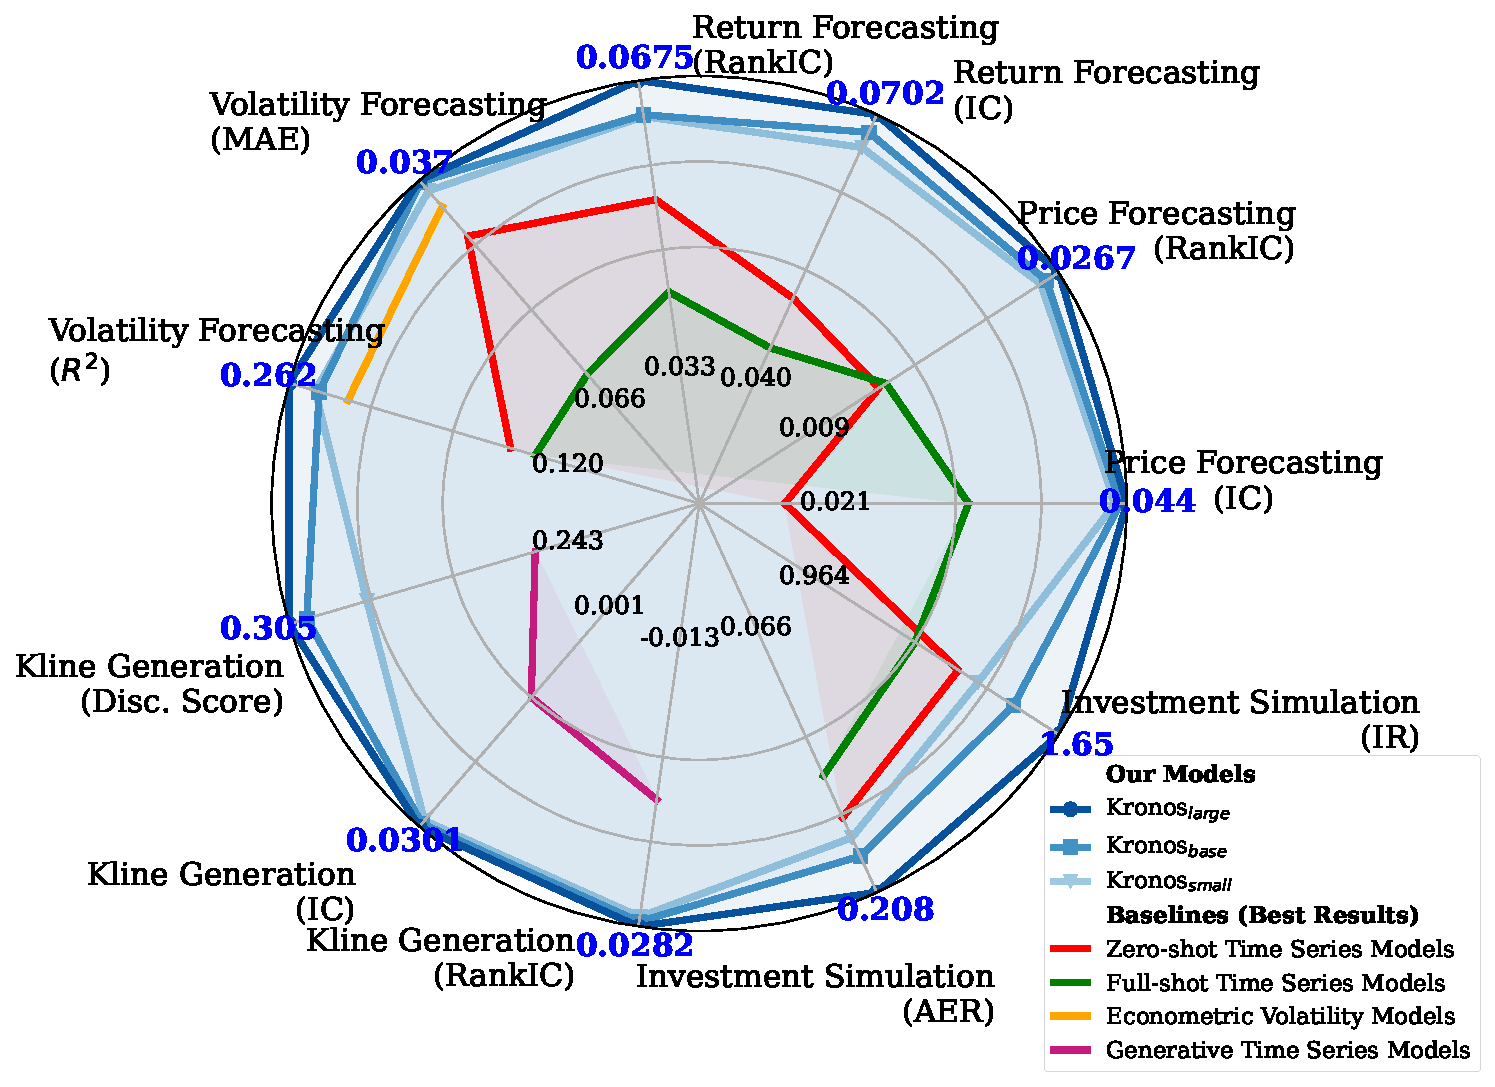
\includegraphics[width=1.0\columnwidth]{img/performance_overview.pdf}
    \caption{여러 정량 금융 과제에서 Kronos의 종합 성능. 이 차트는 우리의 Kronos 모델들(파란색 계열)을 여러 범주의 특화된 베이스라인과 비교한다.
    중심에서 더 멀리 떨어질수록 더 우수한 성능을 의미한다.
    }
    \label{fig:performance_overview}
\end{figure}


그러나 범용 TSFMs를 금융 K-line 데이터에 적용하는 것은 두 가지 주요 요인으로 인해 상당한 도전을 제기한다.
첫째, K-line 시퀀스는 낮은 신호대잡음비, 강한 비정상성, OHLCVA 속성들 사이의 복잡한 고차 의존성~\cite{zhang2025major,baidya2024addressing}과 같은 고유한 통계적 특성을 보이는데, 이는 일반적인 TSFMs의 귀납적 편향과 잘 맞지 않는 경우가 많다.
둘째, 금융 도메인은 주류 TSFM 연구에서 대체로 충분히 다루어지지 않았다; 금융 시퀀스는 대부분의 기존 TSFMs~\cite{das2024decoder,gao2024units,xiaoming2025time}의 사전학습 코퍼스에서 작은 비중만을 차지하며
, 변동성 추정, 합성 시퀀스 생성, 리스크 관리에 걸친 정량 금융에 중요한 다운스트림 과제의 범위는 대체로 해결되지 않은 채 남아 있다. 이러한 요인들은 중요한 관찰로 이어지며, 우리는 이를 본 연구에서 실증적으로 검증한다: 범용 TSFMs는 금융 과제에서 특화된 사전학습되지 않은 모델(예: iTransformer~\cite{liuitransformer})보다 성능이 낮은 경우가 많고, 더 넓은 정량 금융 지형 전반으로 일반화하는 데 실패한다.

이러한 한계를 해결하기 위해, 우리는 \textbf{금융 K-line 데이터를 위해 특별히 설계된 통합적이고 확장 가능한 사전학습 프레임워크인 Kronos}를 소개한다. Kronos는 특화된 토크나이저를 사용하여 연속적인 다변량 K-line 입력을 조밀한 토큰 시퀀스로 이산화하고, 중요한 가격--거래량 상호작용을 보존한다. 이후 45개 이상의 글로벌 시장과 7개의 시간적 세분도에서 추출한 120억 개 이상의 K-line 기록으로 구성된 방대하고 이질적인 코퍼스에서 자기회귀 사전학습을 수행한다.

우리는 다양한 정량 금융 과제 전반에 걸친 포괄적인 실험을 통해 Kronos의 효용성을 검증하며, 그 상위 수준 요약은 Figure \ref{fig:performance_overview}에 제시되어 있다. 핵심 과제인 가격 시계열 예측에서 Kronos는 새로운 state-of-the-art를 수립하며, RankIC를 선도적인 TSFM 대비 93\%, 최고 성능의 사전학습되지 않은 베이스라인 대비 87\% 향상시킨다. 또한 변동성 예측에서 9\% 더 낮은 MAE를 달성하고 합성 K-line 생성의 생성 충실도를 22\% 개선함으로써 강한 범용성을 보여준다. 이러한 결과는 우리의 접근법이 폭넓게 효과적임을 강조하고, 금융 시장의 복잡한 ``언어''를 해석하기 위한 견고한 foundation model로서 Kronos의 잠재력을 부각한다.

우리의 주요 기여는 다음과 같이 요약할 수 있다:

\begin{itemize}
    \item 우리는 계층적 표현을 학습하는 금융 K-line 데이터를 위한 새로운 모델링 프레임워크를 제안한다. 이 프레임워크는 각 다변량 K-line 기록을 구조화된 이중 구성요소(거친 및 세밀한) 토큰으로 양자화하는 특화된 토크나이저와, 이러한 서브토큰을 순차적으로 예측하는 맞춤형 자기회귀 목표를 특징으로 한다. 이 coarse-to-fine 예측 방식은 Kronos가 다중 스케일 시장 동학을 명시적으로 모델링할 수 있게 한다.

    \item 우리는 다양한 용량을 가진 Kronos 모델군에 대해 대규모 사전학습을 수행한다. 이는 45개 이상의 글로벌 거래소에서 수집한 120억 개 이상의 K-line 기록으로 구성된 방대하고 다양한 금융 코퍼스에서 수행되며, 모델들의 효과성을 뒷받침하는 견고하고 일반화 가능한 시장 표현을 학습하는 데 핵심적이다.

    \item 우리는 일련의 정량 금융 과제 전반에 대해 포괄적인 실증 평가를 수행한다. 우리의 결과는 Kronos가 가격 시계열 예측에서 새로운 state-of-the-art를 수립하며, TSFMs와 특화된 베이스라인 모두를 상당히 능가함을 보여준다. 모델의 범용성은 변동성 예측과 합성 K-line 생성을 포함한 더 넓은 범위의 정량 과제에서 보이는 강력한 성능으로 추가 입증된다.
\end{itemize}

\begin{figure*}[t!]
    \centering
    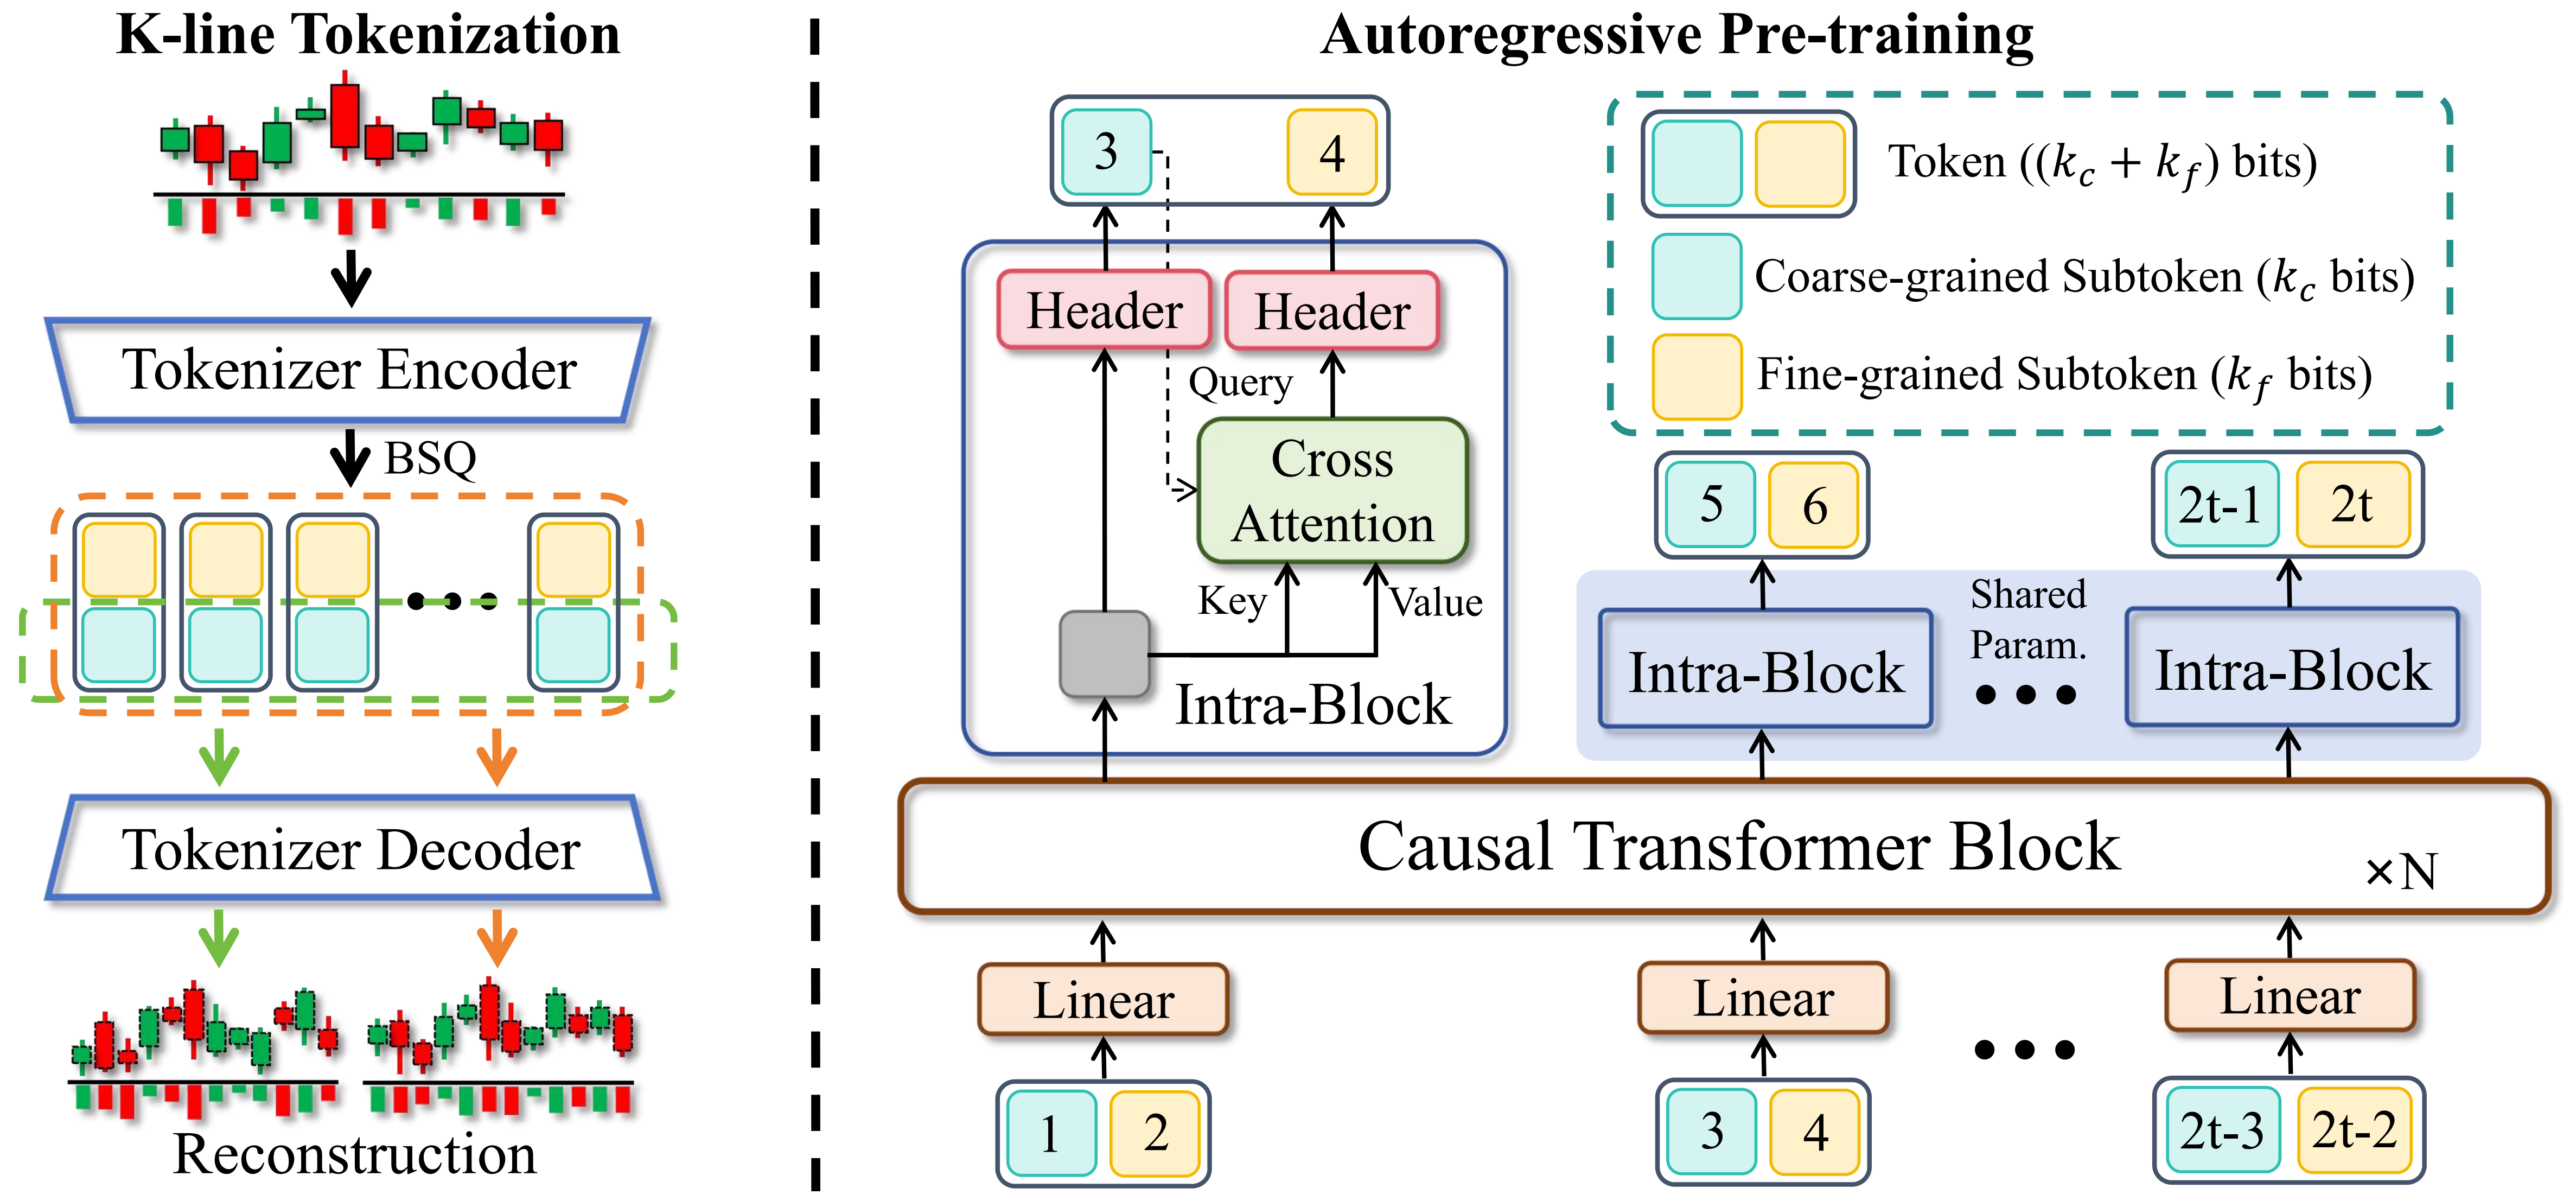
\includegraphics[width=1.0\textwidth]{img/Overview.png}
    \caption{Kronos의 2단계 프레임워크. \textbf{(1) Instance-based K-line Tokenization:} 이중 재구성 목표를 갖는 Transformer 기반 오토인코더가 연속적인 K-line 데이터를 계층적 이산 토큰의 어휘로 양자화하며, 각 토큰은 거친 서브토큰과 세밀한 서브토큰으로 구성된다. \textbf{(2) Autoregressive Pre-training:} decoder-only Transformer는 과거를 조건으로 다음 시점의 계층적 서브토큰을 순차적으로 예측함으로써 시간 동학을 모델링하도록 사전학습된다.}
    \label{fig:overview}
\end{figure*}


\section{Preliminary}

\(D\)차원 벡터 \(\mathbf{x}_t \in \mathbb{R}^D\)가 이산 시간 \(t\)에서의 K-line 관측치를 나타낸다고 하자. 이는 \(D\)개의 핵심 금융 지표로 구성된다. 본 연구에서는 OHLCVA 속성(Open, High, Low, Close 가격, trading Volume, Amount)을 나타내기 위해 차원을 \(D=6\)으로 고정한다. 이러한 입력 선택의 근거는 Appendix~\ref{sec:discussion} (Q1)에 자세히 설명되어 있다. 과거 시퀀스
\(
\mathbf{x}_{1:T} = (\mathbf{x}_1, \mathbf{x}_2, \ldots, \mathbf{x}_T),
\)
가 주어졌을 때, 우리의 목표는 다음 \(H\)개의 관측치
\(
\hat{\mathbf{x}}_{T+1:T+H} = (\hat{\mathbf{x}}_{T+1}, \hat{\mathbf{x}}_{T+2}, \ldots, \hat{\mathbf{x}}_{T+H}).
\)
를 예측하는 것이다.

Kronos는 원시 연속 입력에 직접 작동하는 대신, 먼저 각 다변량 관측치 \(\mathbf{x}_t\)를 이산 토큰 \(b_t\)로, 학습 가능한 코드북 \(\mathcal{C}\)를 통해 양자화한다.
% 이 접근법은 주어진 시점의 전체 OHLCVA 지표 집합을 양자화를 위한 단일 단위로 취급한다.
따라서 원래 시퀀스
\(
\mathbf{x}_{1:T} = (\mathbf{x}_1, \dots, \mathbf{x}_T)
\)
는
\(
\mathbf{b}_{1:T} = (b_1, \dots, b_T).
\)
로 매핑된다. 그러면 예측 과제는 자기회귀 토큰-시퀀스 모델링 문제로 환원된다:
\begin{equation}
\label{eq:ts_ar}
p(\mathbf{b}_{T+1:T+H} \mid \mathbf{b}_{1:T})
= \prod_{h=1}^{H} p\bigl(b_{T+h} \mid \mathbf{b}_{1:T+h-1}\bigr).
\end{equation}

이러한 이산적 정식화는 본질적으로 확장 가능하며, 합성 데이터 생성 및 변동성 예측과 같이 생성적으로 틀 지을 수 있는 다른 과제로 자연스럽게 확장된다.


\section{방법론}

Kronos는 금융 K-line 시퀀스를 이산 언어로 추상화하고, Figure~\ref{fig:overview}에 설명된 두 단계 프레임워크, 즉 \textbf{(1) K-line 토큰화}와 \textbf{(2) 자기회귀 사전학습}을 통해 이를 구현한다. 첫 번째 단계에서는 연속적인 다변량 K-line 시퀀스를 학습 가능한 코드북을 통해 대응되는 이산 토큰 시퀀스로 양자화하기 위해 특화된 Transformer 기반 tokenizer를 설계한다. 각 K-line 항목(OHLCVA)은 개별 인스턴스로 취급되어 이산 토큰으로 양자화된다. 각 토큰은 coarse-grained subtoken과 fine-grained subtoken으로 구성된다.
이 속성은 계층적 재구성 손실을 통해 강제되며, 이는 subtokens가 서로 다른 정보 수준을 모델링하도록 명시적으로 유도함으로써 coarse-to-fine 정보 계층을 형성한다.
두 번째 단계에서는 표준 next-token prediction 목적을 사용하여, 주어진 과거 문맥에 조건화된 각 미래 시점에서 두 subtoken 수준을 순차적으로 예측하도록 이러한 토큰화된 시퀀스에 대해 decoder-only Transformer를 자기회귀적으로 사전학습한다. 이 통합된 \emph{discretize-and-generate} 패러다임은 Kronos가 시장 동학의 고충실도 계층적 표현을 구축할 수 있게 하며, downstream 정량 분석을 위한 견고한 기반을 제공한다.

\subsection{K-line 토큰화}

Kronos의 첫 번째 단계는 OHLCVA 지표를 인코딩하는 $\mathbf{x}_{t}\in\mathbb{R}^{D}$로 이루어진 연속적인 $D$차원 K-line 시퀀스 $\mathbf{x} = (\mathbf{x}_{1}, \ldots, \mathbf{x}_{T})$를 대응되는 이산 토큰열로 변환한다. 이는 encoder $E_{\text{enc}}$, quantizer $Q$, decoder $E_{\text{dec}}$로 구성된 Transformer 기반 autoencoder(Figure~\ref{fig:tokenizer})를 사용하여 달성된다. 생성 모델링의 비디오 양자화 방법~\cite{van2017neural,yu2023language}에서 영감을 받아, 우리는 Binary Spherical Quantization (BSQ)~\cite{zhao2024image}, 즉 Look-up Free Quantization (LFQ)~\cite{yu2023language}의 변형을 이 과제에 맞게 적용한다.
이 선택의 근거는 Appendix~\ref{sec:discussion} (Q2)에서 논의한다.
BSQ는 연속 잠재 벡터 $\bm{\xi}_t$를 학습 가능한 초평면들의 집합에 투영함으로써 $k$-bit 이진 코드 $b_t \in \{-1,1\}^k$로 양자화한다. 풍부한 금융 패턴을 포착하기 위해 큰
bit 수 $k$(예: $k=20$)가 바람직하지만, 이는 크기가 $2^k$인 지수적으로 큰 vocabulary를 초래하여 이후 자기회귀 모델의 계산 비용과 파라미터 크기 측면에서 상당한 문제를 야기한다. 이를 완화하기 위해, 우리는 비디오 양자화 및 생성에 관한 최근 연구~\cite{yu2023language,wang2025bridging}를 따라 $k$-bit 코드를 $n$개의 subspace로 factorize한다. Appendix~\ref{sec:discussion} (Q3)에 자세히 설명된 파라미터 절감과 지연 비용 간의 trade-off에 근거하여, 우리는 $n=2$로 설정한다. 코드를 동일한 bit 길이 $k_c = k_f = k/2$를 갖는 coarse subtoken $b_{t}^{c}$와 fine subtoken $b_{t}^{f}$로 분할하며, 여기서 $k=k_c+k_f$이다. 결과 코드 $b_t$는 이 두 subtokens의 concatenation이다:
\(
  b_{t} = \bigl[b_{t}^{c},\,b_{t}^{f}\bigr],
\)
여기서 $b_{t}^{c}$, $b_{t}^{f} \in\{-1,1\}^{k/2}$이다. 이 분해는 크기가 $2^k$인 큰 vocabulary에 대한 단일 예측을 $2^{k/2}$개 항목에 대한 두 개의 순차 예측으로 변환하여, 계산 및 파라미터 복잡도를 모두 크게 줄인다.

각 토큰 내부에 coarse-to-fine 구조를 강제하기 위해, 우리는 계층적 재구성 손실과 BSQ를 위한 commitment loss를 결합한 복합 목적함수로 tokenizer를 학습한다:
\begin{equation}
  \mathcal{L}_{\text{tokenizer}}
  = \mathcal{L}_{\text{coarse}} + \mathcal{L}_{\text{fine}} + \lambda \mathcal{L}_{\text{quant}},
\end{equation}
여기서 $\lambda$는 균형을 조절하는 hyperparameter이다. 구성 요소는 다음과 같이 정의된다:
\begin{itemize}
    \item \(\mathcal{L}_{\text{coarse}} = \mathbb{E}\bigl[\|\mathbf{x} - E_{\text{dec}}(\mathbf{b}^{c})\|^{2}\bigr]\), 이는 coarse subtoken \(\mathbf{b}^{c}\)가
    % 독립적인,
    낮은 충실도의 재구성을 형성하도록 학습한다.
    \item \(\mathcal{L}_{\text{fine}} = \mathbb{E}\bigl[\|\mathbf{x} - E_{\text{dec}}(\mathbf{b})\|^{2}\bigr]\), 이는 완전한 토큰 \(\mathbf{b}\)을 사용한 높은 충실도의 재구성을 평가한다.
    \item \(\mathcal{L}_{\text{quant}}\)는 학습 과정을 정규화하는 BSQ~\cite{zhao2024image}의 quantization loss이다.
    % 이는 연속 잠재 벡터 $\bm{\xi}$와 그 양자화된 이진 대응물 $\mathbf{b}$ 사이의 L2 거리를 패널티로 부과하여, encoder의 출력이 학습된 이산 표현에 가깝게 유지되도록 장려하고 안정적인 학습을 보장한다.
    이는 연속 잠재 벡터 $\bm{\xi}$와 그 이진 코드 $\mathbf{b}$ 사이의 L2 거리를 패널티로 부과하여, encoder의 출력을 학습된 codebook과 정렬함으로써 안정적인 학습을 보장한다.
\end{itemize}

이 계층적 재구성 목적은 우리의 설계에서 핵심적이다. \(\mathcal{L}_{\text{coarse}}\)를 최적화함으로써, coarse subtoken \(\mathbf{b}^{c}\)는 입력의 주요 구조를 포착하도록 학습한다. 결과적으로 \(\mathcal{L}_{\text{fine}}\)을 최적화하는 동안, fine-grained subtoken \(\mathbf{b}^{f}\)는 coarse approximation을 정교화하는 데 필요한 잔차 정보를 인코딩하도록 유도된다. 선행 연구는 coarse-to-fine 디코딩 순서가 생성 품질을 향상시킨다는 것을 보였다~\cite{wang2025bridging}. 본질적으로 coarse 정보를 포함하는 토큰을 식별하고 그 디코딩을 우선시하는 대신, 우리의 접근법은 양자화 과정에서 이러한 계층을 토큰 안에 명시적으로 부여하도록 설계되었다. 이는 첫 번째 subtoken이 항상 coarse-grained 정보를 나타내도록 보장하여, 이후 자기회귀 모델링 단계에 필요한 조건부 의존성을 확립한다.


\begin{figure}[t]
    \centering
    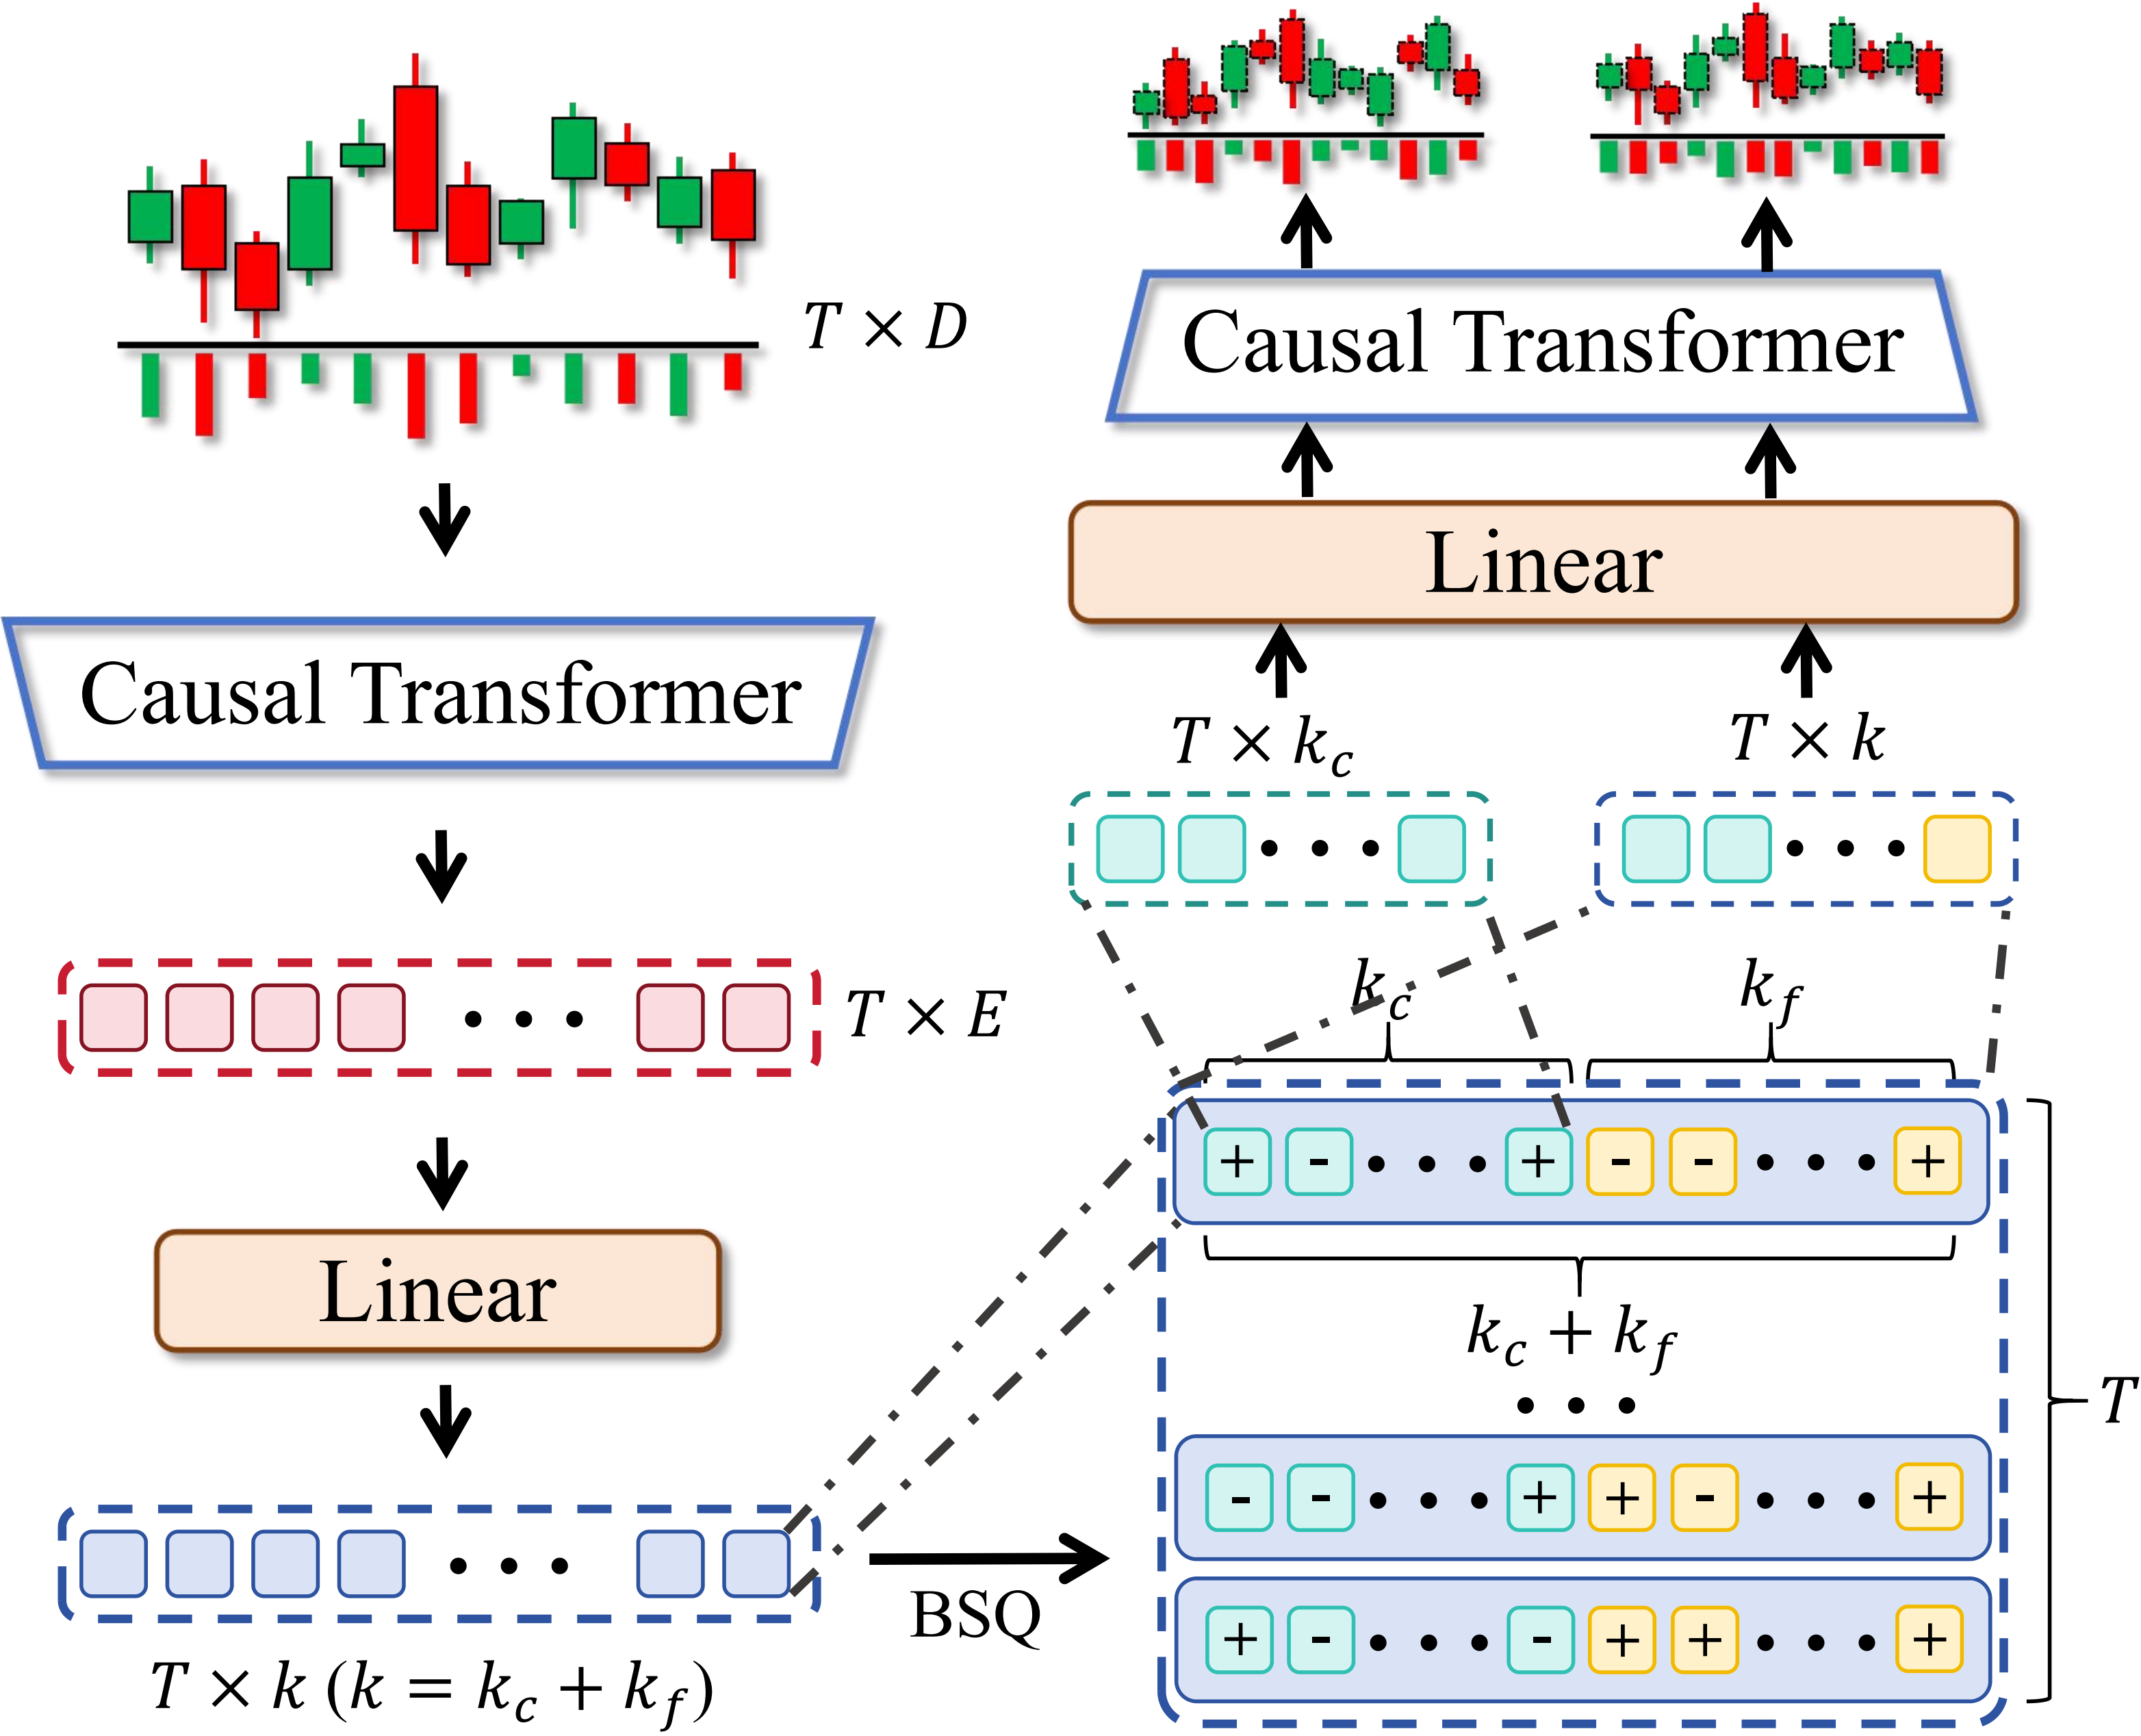
\includegraphics[width=1.0\columnwidth]{img/Tokenizer.png}
    \caption{K-line Tokenizer의 구조. 이는 Binary Spherical Quantization (BSQ) layer를 갖춘 Transformer 기반 autoencoder를 사용한다.
    % 복합 손실 목적($\mathcal{L}_{\text{coarse}}, \mathcal{L}_{\text{fine}}, \mathcal{L}_{\text{quant}}$)은 각 토큰 내부의 coarse-to-fine 표현 구조 학습을 유도한다.
    }
    \label{fig:tokenizer}
\end{figure}

\subsection{계층적 자기회귀 모델링}
\label{sec:autoregressive}

토큰화 단계 이후, 결과로 얻어진 이산 시퀀스는 $E_{\text{ar}}$로 표기되는 decoder-only Transformer를 사용해 모델링되며, 이 모델은 각 시점의 예측이 과거 문맥에만 의존하도록 causal-attention을 사용한다. 주요 목표는 토큰 시퀀스 $\mathbf{b} = \{b_1, \dots, b_T\}$에 대한 joint distribution을 추정하는 것이다. Equation~\ref{eq:ts_ar}의 단순화된 형태는 다음과 같이 유도될 수 있다:
\begin{equation}
    p(\mathbf{b}) = \prod_{t=1}^{T} p(b_t | \mathbf{b}_{<t}),
\end{equation}
여기서 $\mathbf{b}_{<t}$는 시간 $t-1$까지의 모든 이전 토큰을 나타낸다.

각 토큰이 $b_t = [b_t^{c}, b_t^{f}]$로 구조화되는 계층적 토큰 설계를 고려하여, 우리는 내재된 coarse-to-fine 의존성을 명시적으로 포착하기 위해 chain rule을 사용해 conditional probability를 추가로 분해한다:
\begin{equation}
\label{eq:chain_rule}
p(b_t | \mathbf{b}_{<t}) = p(b_t^{c} | \mathbf{b}_{<t}) \cdot p(b_t^{f} | \mathbf{b}_{<t}, b_t^{c}).
\end{equation}
이 공식화는 모델이 먼저 coarse-grained subtoken을 예측하도록 하며, 이는 이후 fine-grained residual subtoken을 생성하기 위한 scaffold 역할을 한다. 따라서 사전학습 목적은 이러한 계층적 factorization 하에서 관측된 시퀀스의 log-likelihood를 최대화하는 것으로 귀결된다.

Figure~\ref{fig:overview} (Right)에 나타난 바와 같이, 자기회귀 과정은 각 시점에 대한 통합 입력 벡터를 구성하는 것에서 시작한다. 구체적으로 시간 $i$에서 subtokens $b_i^{c}$와 $b_i^{f}$는 서로 다른 두 embedding layer를 사용해 각각 벡터 표현으로 독립적으로 투영되어, 각각 $e_c(b_i^{c})$와 $e_f(b_i^{f})$ 표현을 생성한다. 그런 다음 이러한 embeddings를 concatenate하고 선형 투영하여 융합된 입력 벡터를 생성한다:
\begin{equation}
\label{eq:embedding}
    \mathbf{v}_i = W_{\text{fuse}}([e_c(b_i^{c}); e_f(b_i^{f})]),
\end{equation}
여기서 $[\cdot;\cdot]$는 concatenation을 나타내며, $W_{\text{fuse}}$는 결합된 표현을 모델의 latent space로 투영하는 학습 가능한 weight matrix이다.

융합된 입력 시퀀스 $\{\mathbf{v}_1, \dots, \mathbf{v}_{t-1}\}$는 Transformer $E_{\text{ar}}$에 의해 처리되어 contextualized hidden states를 출력한다. $\mathbf{b}_{< t}$를 처리하여 얻은 최종 hidden state는 $\mathbf{h}_t$로 표기되며, 이후 토큰 $b_t$를 예측하는 데 사용된다. 이 hidden state는 다음 단계에서 coarse 및 fine subtokens 모두의 자기회귀 예측에 정보를 제공하여, 모델이 데이터에 내재된 multi-scale temporal dependencies를 효과적으로 포착할 수 있게 한다.

\textbf{Coarse Subtoken 예측.} History vector $\mathbf{h}_t$는 선형 head $W_c$에 의해 투영되어 첫 번째 subtoken distribution에 대한 logits를 생성한다:
\begin{equation}
    p(b_{t}^{c} | \mathbf{b}_{< t}) = \text{softmax}(W_c \mathbf{h}_t)
\end{equation}

\textbf{Fine Subtoken 예측.} Equation~(\ref{eq:chain_rule})의 conditional dependency를 모델링하기 위해, 문맥은 예측된 coarse subtoken $\hat{b}_{t}^{c}$로 업데이트되어야 한다. 학습 중에는 ground-truth subtoken(즉, teacher-forcing)을 사용하는 대신, 예측 분포 $p(b_{t}^{c} | \mathbf{b}{< t})$에서 샘플링된 이전 단계의 모델 자체 예측 $\hat{b}_{t}^{c}$를 사용한다. 우리는 이러한 샘플링 전략이 exposure bias를 완화하여 모델 견고성을 향상시키고, ground-truth tokens를 사용할 수 없는 multi-step inference의 auto-regressive 특성과 학습 분포를 더 잘 정렬한다고 본다. 우리는 $\hat{b}_{t}^{c}$의 embedding이 query로 작용하고 history $\mathbf{h}_t$가 key와 value를 제공하는 cross-attention mechanism을 사용한다. 그 결과는 두 번째 head $W_f$에 의해 투영된다:
\begin{equation}
\begin{aligned}
    \mathbf{h}^{\text{update}}_t = \text{CrossAttn}&(q=e_c(\hat{b}_{t}^{c}), k=v=\mathbf{h}_t) \\
    p(b_{t}^{f} | \mathbf{b}_{< t}, b_{t}^{c}) &= \text{softmax}(W_f \mathbf{h}^{\text{update}}_t)
\end{aligned}
\end{equation}
전체 학습 목적 $\mathcal{L}_{\text{ar}}$는 두 예측 단계에 대해 합산된 데이터의 negative log-likelihood이다:
\begin{equation}
    \mathcal{L}_{\text{ar}} = - \mathbb{E}_{\mathbf{b} \sim \mathcal{D}} \sum_{t=1}^{T} \left[ \log p(b_t^{c} | \mathbf{b}_{<t}) + \log p(b_t^{f} | \mathbf{b}_{<t}, b_t^{c}) \right]
\end{equation}
여기서 $\mathcal{D}$는 data distribution을 나타낸다.

\begin{table}[t]
\centering
\setlength{\tabcolsep}{4pt}

\resizebox{\columnwidth}{!}{%
  \begin{tabular}{l ccccc c}
  \toprule
  & 레이어 & $\mathbf{d}_{\text{model}}$ & $\mathbf{d}_{\text{ff}}$ & 헤드 & 어휘 ($2^k$) & 파라미터 \\
  \midrule
\text{Kronos}$_{small}$ & 8 & 512  & 1024 & 8 & 20 & 24.7M \\
\text{Kronos}$_{base}$  & 12 & 832 & 2048 & 16 & 20 & 102.3M \\
\text{Kronos}$_{large}$ & 18 & 1664 & 3072 & 32 & 20 & 499.2M \\
  \bottomrule
  \end{tabular}%
}
\caption{Kronos family의 model configurations. Transformer layers 수, model dimension ($\mathbf{d}_{\text{model}}$), feed-forward dimension ($\mathbf{d}_{\text{ff}}$), attention heads 수, vocabulary size, 그리고 총 parameters 수를 상세히 제시한다.}
\label{tab:kronos_configs_resized}
\end{table}

\subsection{모델 사전학습}

\begin{figure*}[t!]
    \centering
    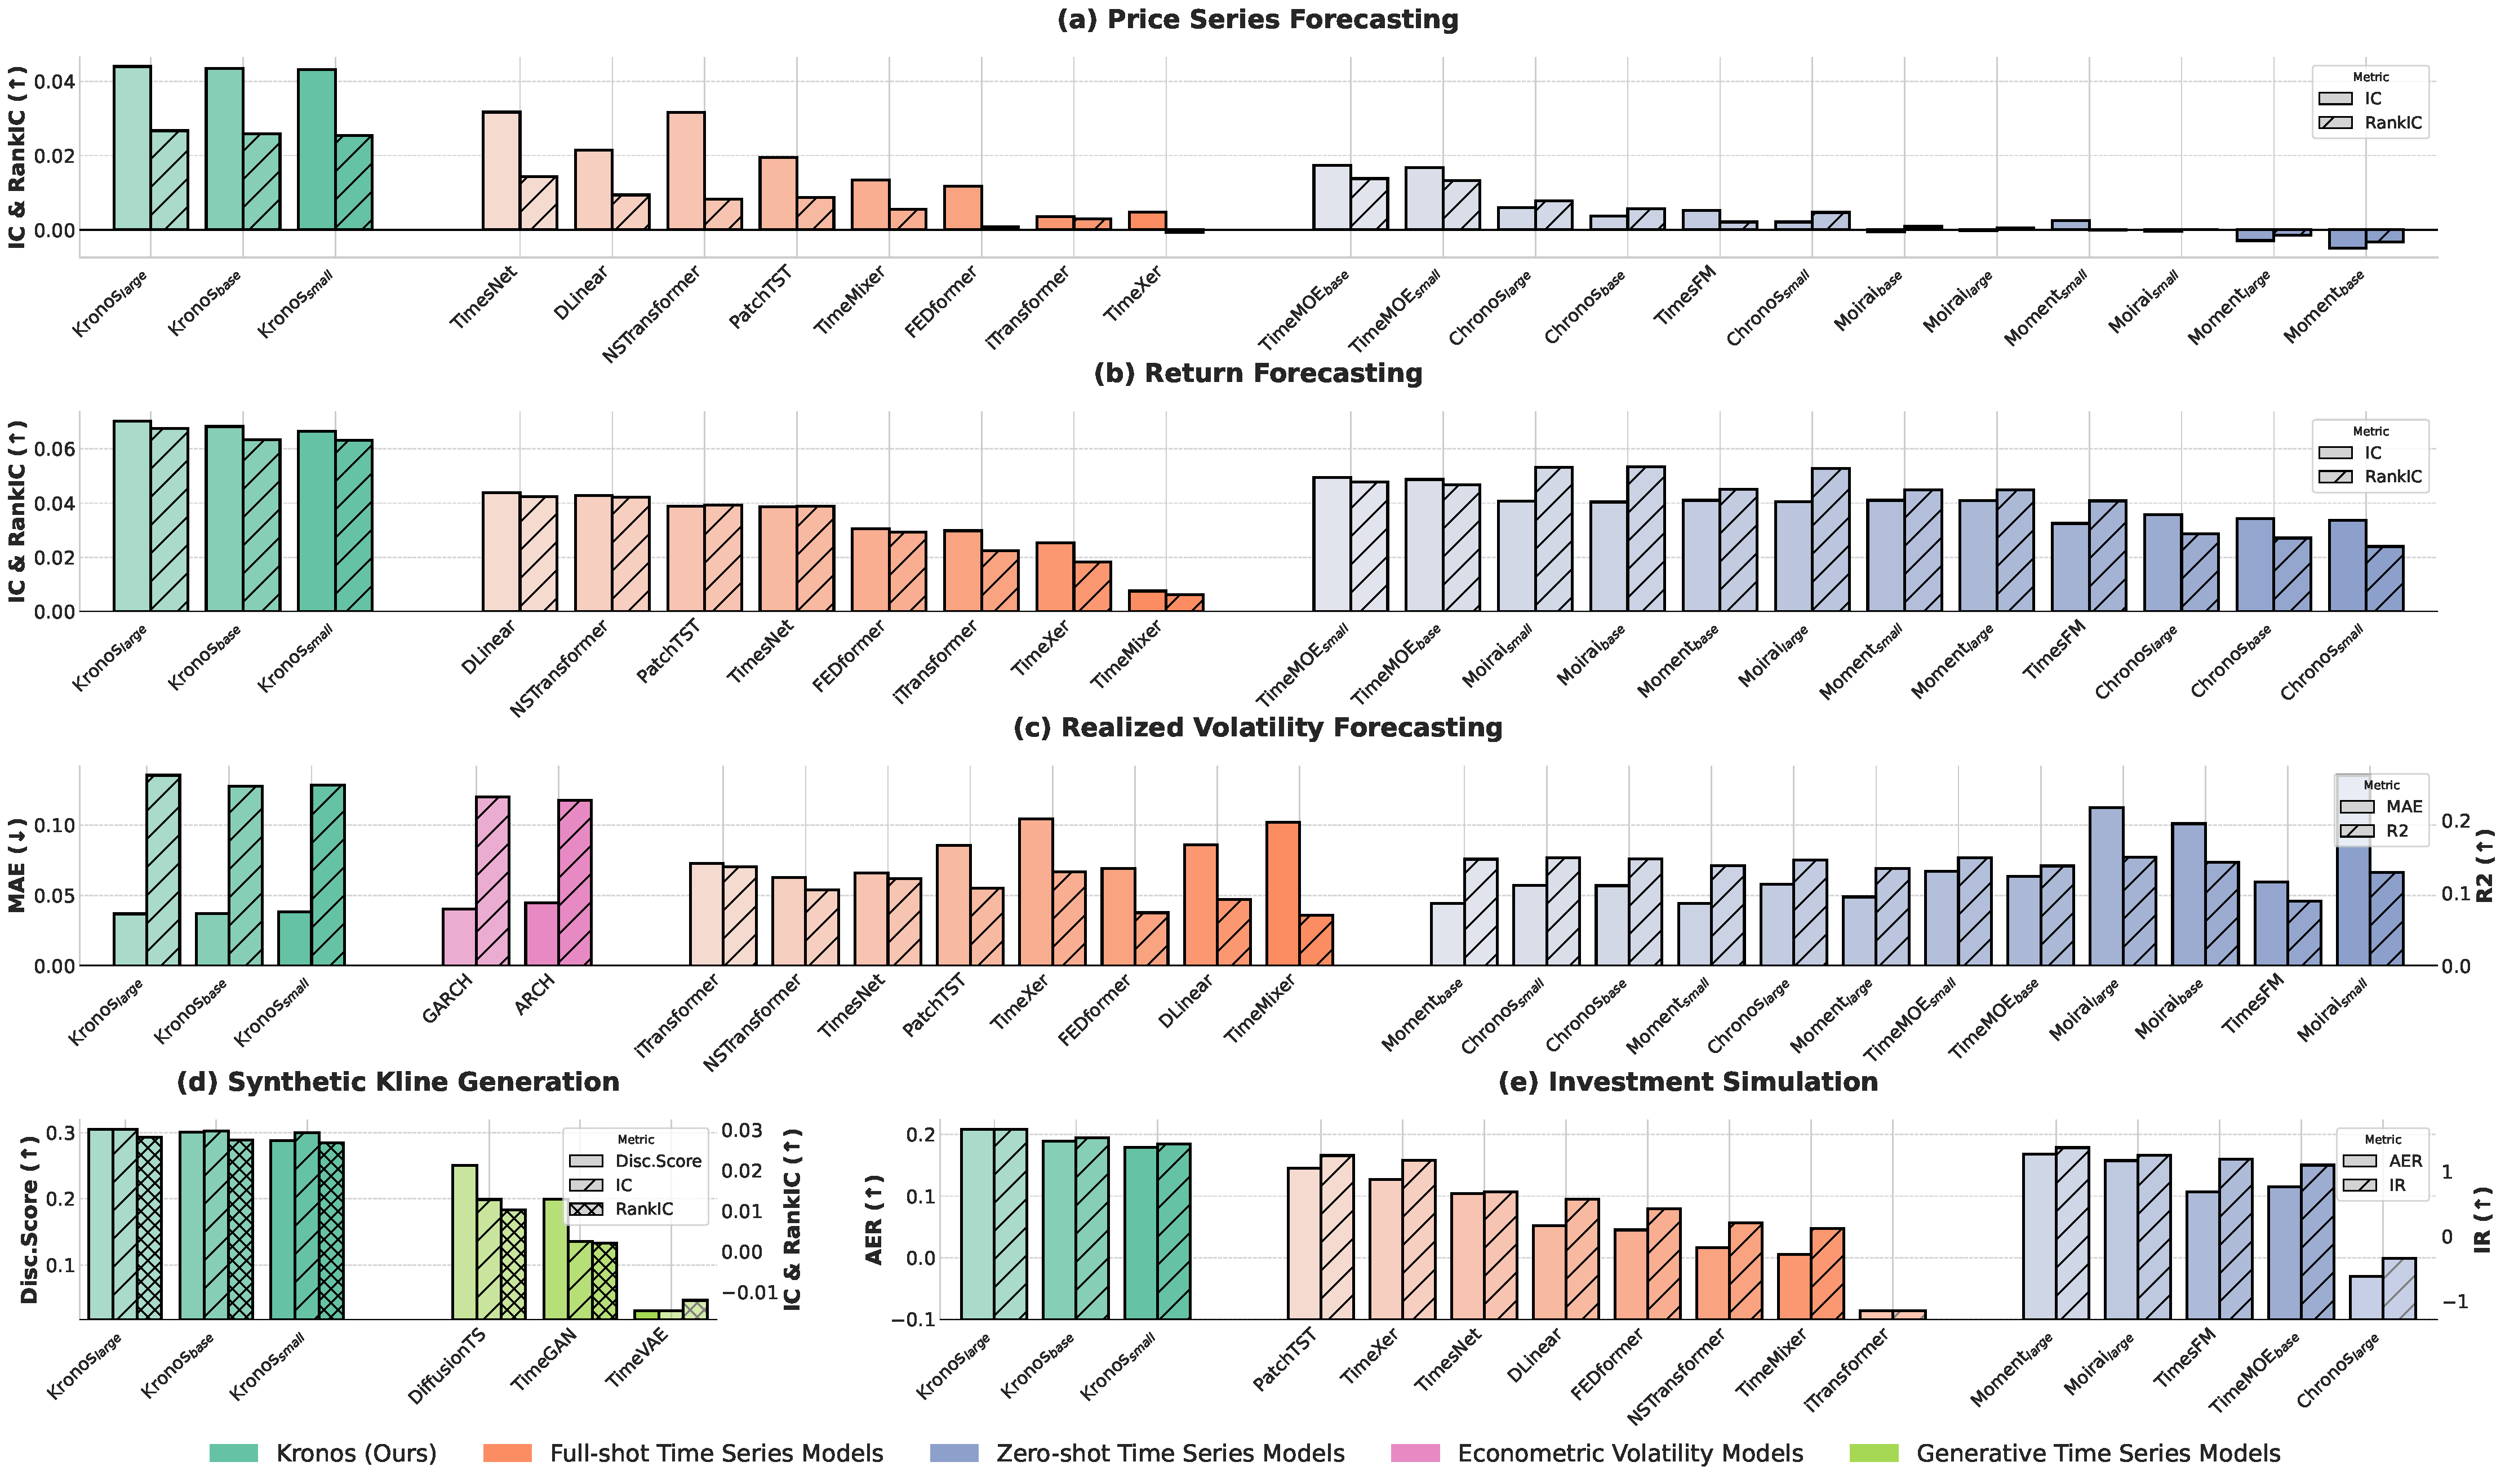
\includegraphics[width=1.0\textwidth]{img/main_result.pdf}
    \caption{다섯 가지 대표 금융 과제 전반의 주요 실험 결과. Subfigures (a-c)는 price series, returns, realized volatility에 대한 forecasting performance를 보여준다. Subfigure (d)는 fidelity와 usefulness 측면의 generative model performance를 나타낸다. Subfigure (e)는 investment simulation backtesting results를 제시한다.}
    \label{fig:main_result}
\end{figure*}

\paragraph{데이터셋}
사전학습의 품질을 보장하기 위해, 우리는 대규모 고품질 금융 K-line dataset을 처음부터 구축한다. 잘 정제된 공개 datasets를 쉽게 모을 수 있는 일반 time series에 대한 foundation-model 연구와 달리, 포괄적이고 고품질인 금융 데이터는 여전히 제한적이다. 우리의 dataset은 7개의 sampling frequencies에 걸쳐 120억 개가 넘는 observations를 포함하며, 45개 글로벌 exchanges에서 수집된 광범위한 asset classes를 포괄한다. 데이터 품질을 보장하기 위해, 우리는 금융 K-line 데이터의 고유한 특성에 맞춘 간소화된 data-cleaning pipeline을 개발하며, 이는 비정상적인 price spikes나 장기간의 inactivity와 같은 저품질 segments를 식별하고 필터링한다. Cleaning pipeline에 대한 추가 세부 사항은 Appendix~\ref{sec:dataset_details}에서 확인할 수 있다.

\paragraph{모델 학습} LLM에서 관찰된 scaling laws~\cite{kaplan2020scaling}에 근거하여, 우리는 성능과 inference budget 사이의 trade-off를 제공하기 위해 parameter count를 증가시킨 세 가지 Kronos variants를 거의 0.5 billion까지 학습했다. 자세한 model configurations는 Table~\ref{tab:kronos_configs_resized}에 제시되어 있다.
자원 제약과 실제 deployment scenarios를 고려하여, 우리는 최대 context length를 512 tokens로 제한한다. 그럼에도 이 설계는 다양한 frequencies의 K-line 데이터를 활용함으로써 임의의 forecasting horizons와 완전히 호환된다. 예를 들어, 단기 forecasting에는 1-minute data를 사용하고 weekly 또는 monthly predictions에는 daily data를 사용할 수 있다. 전체 training details는 Appendix~\ref{sec:implementation_details}에 제공된다.

\paragraph{추론} Inference 시에는 text generation과 유사하게 미래 token sequences를 자기회귀적으로 생성한다. 이 과정의 stochasticity는 temperature scaling 및 top-$p$ (nucleus) sampling~\cite{holtzman2019curious}과 같은 표준 기법을 통해 제어된다. Logits $\mathbf{z}$에서 token $i$를 샘플링할 확률은 $p_i \propto \exp(z_i / T)$로 주어지며, 여기서 $T$는 temperature이다. 높은 precision이 필요한 과제의 경우, 여러 future trajectories(즉, Monte Carlo rollouts)를 생성하고 decoded continuous values를 평균하여 더 안정적인 forecast를 생성함으로써 prediction accuracy를 향상시킬 수 있다. 우리의 실험에서 입증된 바와 같이, 이 접근법은 forecast quality를 일관되게 개선한다.


\section{실험}
\label{sec:experiments}

\begin{table*}[t!]

\resizebox{\textwidth}{!}{
\begin{tabular}{@{} l l l c c c c c c c c @{}}
\toprule

\multirow{2.5}{*}{\textbf{모델}} & \multirow{2.5}{*}{\textbf{예측 공간}} & \multirow{2.5}{*}{\textbf{학습 목적 함수}} & \multicolumn{2}{c}{\textbf{가격 시계열 예측}} && \multicolumn{2}{c}{\textbf{수익률 예측}} && \multicolumn{2}{c}{\textbf{변동성 예측}} \\
\cmidrule(lr){4-5} \cmidrule(lr){7-8} \cmidrule(lr){10-11}

& & & IC ($\uparrow$) & RankIC ($\uparrow$) && IC ($\uparrow$) & RankIC ($\uparrow$) && MAE ($\downarrow$) & R$^2$ ($\uparrow$) \\
\midrule

Direct-AR       & 연속형 & 평균제곱오차 (MSE)  & 0.0212 & 0.0149 && 0.0416 & 0.0399 && 0.0565 & 0.1608 \\
Prob-AR         & 연속형 & 음의 로그가능도 (NLL) & 0.0179 & 0.0102 && 0.0356 & 0.0329 && 0.0464 & 0.1383 \\
\midrule

Kronos-Parallel & 이산형   & 교차 엔트로피             & 0.0345 & 0.0226 && 0.0529 & 0.0505 && 0.0461 & 0.1784 \\
\textbf{$\text{Kronos}_{small}$} & \textbf{이산형}   & \textbf{교차 엔트로피}    & \textbf{0.0431} & \textbf{0.0254} && \textbf{0.0665} & \textbf{0.0622} && \textbf{0.0384} & \textbf{0.2490} \\
\bottomrule
\end{tabular}
}
\centering
\caption{
    Kronos의 아키텍처 선택을 세분화해 분석한 제거 연구.
    우리는 서로 다른 \textbf{예측 공간}(연속형 vs. 이산형)과 이에 대응하는 \textbf{학습 목적 함수}를 대상으로 하는 변형들과 우리 모델을 비교한다.
    \textit{Direct-AR}은 표준 회귀 기준선 역할을 한다.
    \textit{Prob-AR}은 연속 공간에서 확률적 모델링의 이점을 평가한다.
    \textit{Kronos-Parallel}은 서브토큰을 동시에 예측함으로써 우리의 순차적 서브토큰 설계를 제거한 변형이다.
    % 화살표($\uparrow$/$\downarrow$)는 선호되는 방향을 나타낸다.
    최상의 결과는 \textbf{굵게} 표시한다.
}
\label{tab:ablation_study_refined}
\end{table*}

\begin{figure*}[htbp]
    \centering
    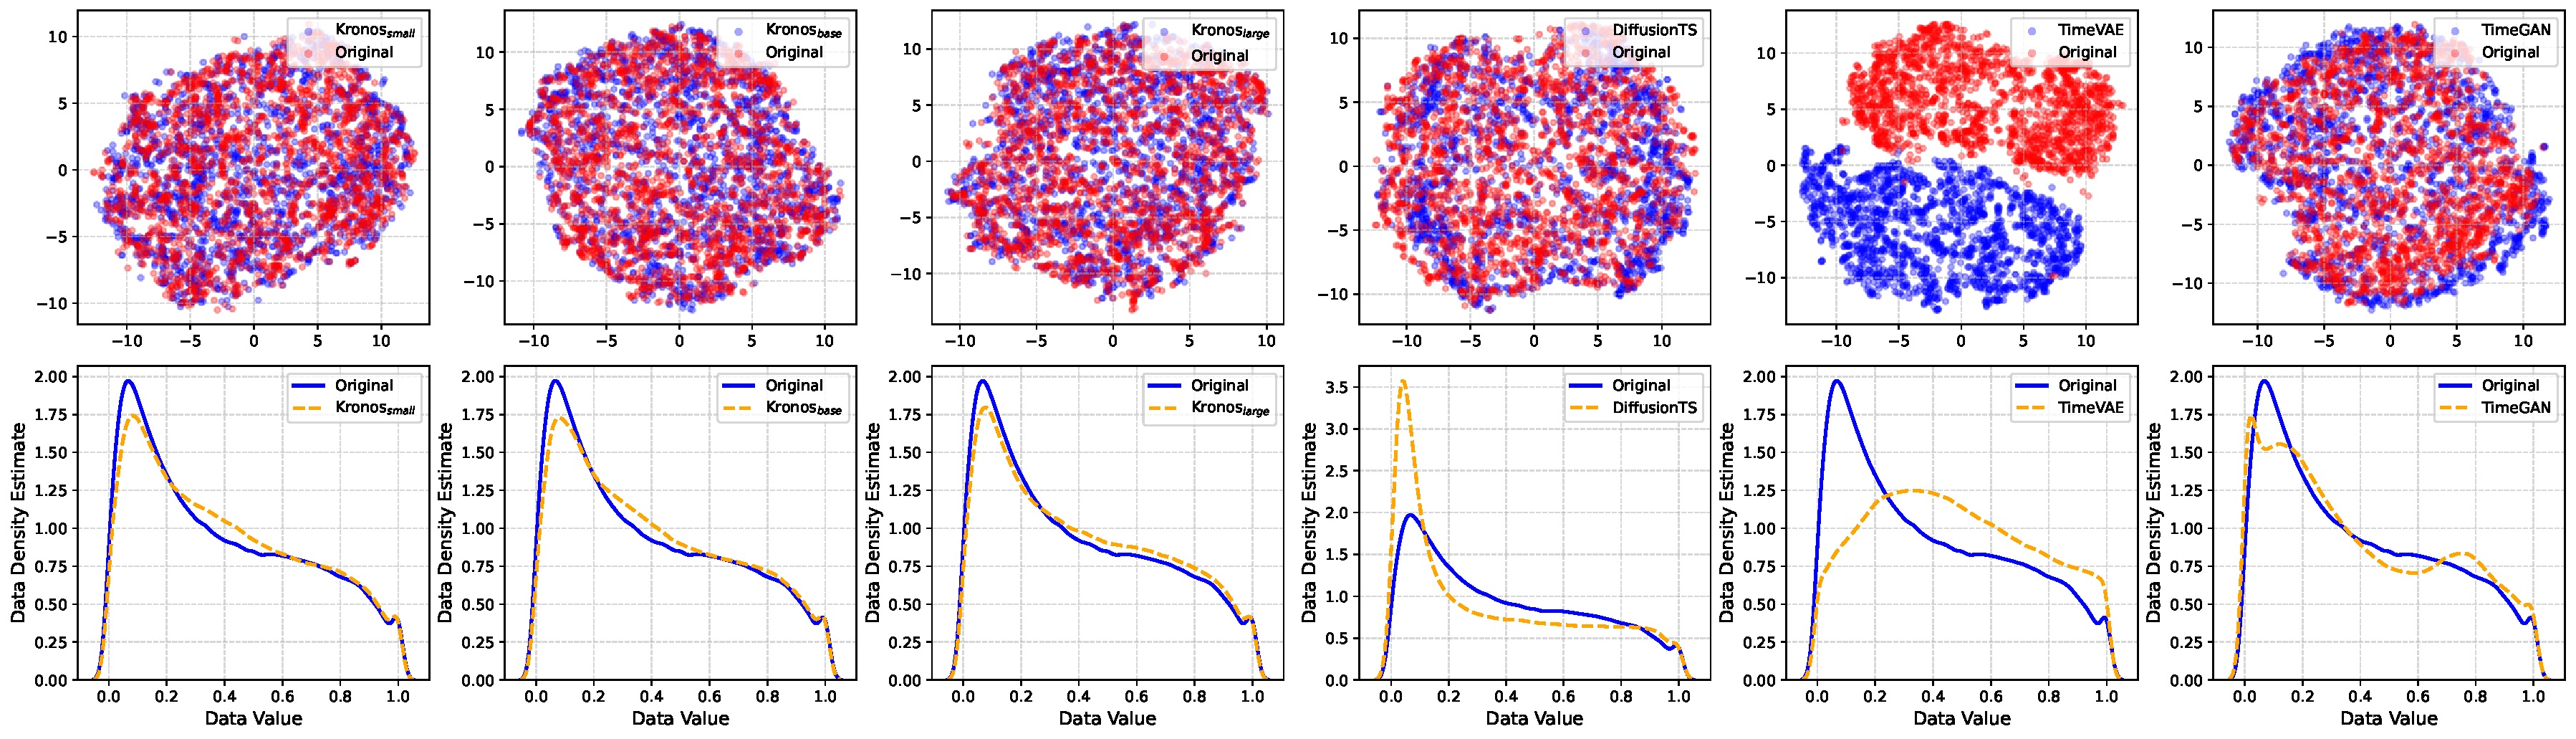
\includegraphics[width=1.0\textwidth]{img/gen_diversity_XSHG_15min.pdf}
    \caption{상하이증권거래소 데이터셋(15분 빈도)에서 생성 모델들의 시각적 비교.
    \textbf{상단 행:} 원본(\textcolor{red}{빨간색}) 데이터와 합성(\textcolor{blue}{파란색}) 데이터의 t-SNE 임베딩.
    \textbf{하단 행:} 원본 데이터와 합성 데이터의 커널 밀도 추정(KDE).}
    \label{fig:gen_diversity_XSHG_15min}
\end{figure*}

금융 K-line 데이터의 기반 모델로서 Kronos의 능력을 종합적으로 평가하기 위해, 우리는 5개의 대표 과제에 걸친 일련의 실험을 설계한다. 이러한 과제들은 예측 및 생성 응용 모두에서 Kronos의 성능을 평가하도록 선정되었으며, 이를 통해 실제 정량 금융 시나리오에서의 다재다능함을 입증한다.

\subsection{실험 설정}

실험 과제는 예측 응용(가격 시계열, 수익률 및 실현 변동성 예측), 생성 능력(합성 K-line 생성), 그리고 실제 적용 가능성을 가늠하기 위한 투자 시뮬레이션을 포괄한다.

엄밀한 비교를 위해, 우리는 25개의 기준 모델로 구성된 포괄적인 모음과 Kronos를 벤치마크한다. 이러한 기준선은 네 가지 서로 다른 패러다임 전반의 최신 기술을 대표하도록 신중히 선정되었다: 사전학습되지 않은 full-shot 모델(예: iTransformer~\cite{liuitransformer}), zero-shot time series foundation model(예: TimeMOE~\cite{xiaoming2025time}), 계량경제학적 변동성 모델(예: GARCH~\cite{bollerslev1986generalized}, 계량경제학의 변동성 예측을 위한 고전적 접근법), 그리고 생성형 시계열 모델(예: DiffusionTS~\cite{yuan2024diffusion}).
과제 세부사항과 기준선은 부록~\ref{sec:exp_setup_details}에 제시되어 있다. 주요 실험 결과의 개요는 그림~\ref{fig:main_result}에 제시되어 있으며, 전체 결과 세부 내역은 부록~\ref{sec:full_exp_results}에 있다.


\subsection{주요 결과}

\subsubsection{예측 과제}
그림~\ref{fig:main_result}(a-c)는 세 가지 예측 과제의 결과를 제시한다. Kronos는 이들 모두에서 일관되게 최첨단 성능을 달성한다. 특히 가격 시계열 예측에서 Kronos는 가장 강력한 TSFM 기준선 대비 RankIC에서 놀라운 93\% 향상을 달성하고, 최고의 사전학습되지 않은 모델 대비 87\%의 이득을 얻는다. 또한 모델 크기가 커질수록 이러한 과제에서의 성능이 일관되게 향상되어, time series foundation model의 scaling laws를 실증적으로 검증한다~\cite{yao2024towards}.


\subsubsection{생성 과제}

확립된 관행~\cite{yoon2019time}에 따라, 우리는 합성 데이터의 품질을 세 가지 관점, 즉 \textit{다양성}, \textit{충실도}, \textit{유용성}에서 평가한다.
\textit{다양성}—생성된 샘플이 실제 데이터의 분포를 얼마나 잘 포괄하는지—을 평가하기 위해, 우리는 두 가지 시각적 방법을 사용한다: t-SNE를 사용해 원본 및 합성 데이터를 2D 공간에 투영하고, 커널 밀도 추정(KDE)을 통해 이들의 분포를 비교한다. 그림~\ref{fig:gen_diversity_XSHG_15min} 및 부록~\ref{sec:full_exp_results}에 나타난 바와 같이, t-SNE 플롯은 Kronos의 합성 데이터가 원본 데이터 공간과 더 잘 겹침을 보여주며, KDE 플롯은 분포의 더 높은 유사성을 확인해 준다.

정량적 평가를 위해, 우리는 판별 점수를 사용하여 \textit{충실도}(즉, 데이터 현실성)를 평가한다. 이 점수는 분류기가 원본 샘플과 합성 샘플을 구별하는 것이 얼마나 어려운지를 측정한다. 또한 Train-on-Synthetic, Test-on-Real (TSTR) 프로토콜을 통해 \textit{유용성}(다운스트림 모델 학습을 위한 합성 데이터의 효과)을 평가한다. 여기서는 예측 모델을 합성 데이터로 학습하고, 실제 데이터로 구성된 테스트 세트에서 그 결과 IC와 RankIC를 평가한다. 그림~\ref{fig:main_result}(d)에 나타난 바와 같이, Kronos는 \textit{충실도}와 \textit{유용성} 모두에서 최고의 성능을 달성한다. 이러한 우수성은 모델 크기가 커질수록 또한 강화된다.

\subsubsection{투자 시뮬레이션}
현실적인 투자 시나리오에서 Kronos의 성능을 검증하기 위해, 우리는 각 모델의 예측 신호로 순위를 매긴 상위-$k$ 종목으로 포트폴리오를 구성하여 중국 A-shares 시장에서 long-only 투자 전략을 시뮬레이션한다.
그림~\ref{fig:main_result}(e)에 나타난 바와 같이, Kronos는 모든 다른 기준선을 능가하며 가장 높은 Annualized Excess Return (AER)과 Information Ratio (IR)를 달성한다. 이는 모델이 우수한 예측 정확도를 실질적인 투자 수익으로 효과적으로 전환할 수 있음을 보여준다.

\subsection{제거 연구}

우리는 핵심 설계 선택을 검증하기 위해 두 가지 질문에 초점을 맞춘 제거 연구를 수행한다: (Q1) 다른 대안들과 비교한 우리의 모델링 패러다임의 효과성, 그리고 (Q2) 어휘 크기의 영향. tokenizer에 대한 추가 제거 연구는 부록~\ref{sec:tokenizer_ablation}에 제공된다.

\noindent\textbf{모델링 패러다임 분석.}
Q1을 다루기 위해, 우리는 비슷한 파라미터 수를 유지하면서 예측 공간과 목적 함수가 다른 변형들과 Kronos를 비교한다. (표~\ref{tab:ablation_study_refined}).
이러한 아키텍처 변형에 대한 자세한 설명은 부록~\ref{sec:ablation_baselines}에 제공된다. 우리는 두 가지 연속 공간 모델, 즉 \textit{Direct-AR}(MSE를 사용하는 회귀 기준선)과 \textit{Prob-AR}을 테스트한다. 확립된 연구~\cite{yao2024towards}에 따라, \textit{Prob-AR}은 heavy-tailed 데이터 분포를 더 잘 모델링하기 위해 Student-t 혼합 분포를 사용한다. 결과는 우리의 이산 공간 모델들이 이러한 연속형 대안들을 현저히 능가함을 보여준다. 또한 서브토큰을 동시에 예측하는 변형인 \textit{Kronos-Parallel}이 우리의 순차적 접근법보다 성능이 낮다는 점도 발견했으며, 이는 서브토큰 의존성을 모델링하는 것의 중요성을 보여준다.
이러한 발견은 이 영역에서 우리의 이산적이고 순차적인 모델링 프레임워크가 더 효과적인 접근법임을 검증한다.



\begin{figure}[t!]
    \centering
    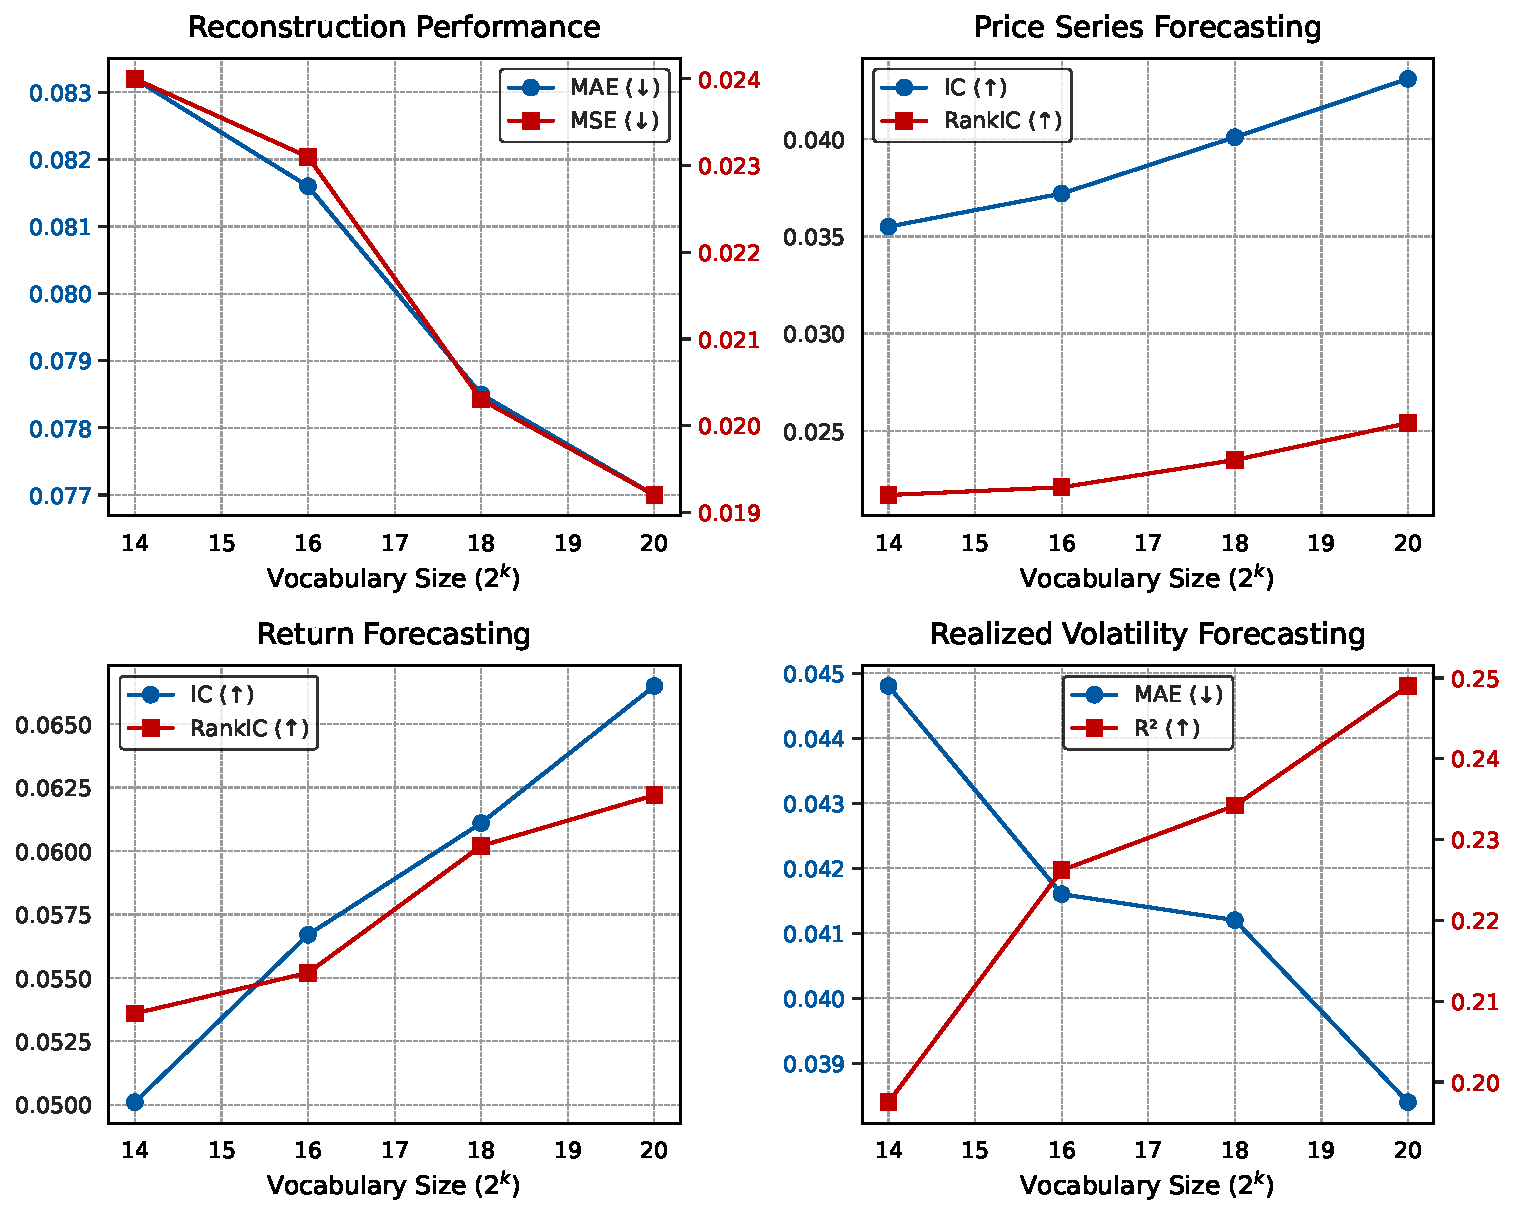
\includegraphics[width=1.0\columnwidth]{img/model_performance_vs_vocab_size.pdf}
    \caption{어휘 크기가 모델 성능에 미치는 영향. 우리는 어휘 크기가 증가함에 따라 재구성 품질과 다운스트림 예측 성능을 플롯한다.
    }
    \label{fig:vocab_size}
\end{figure}

\noindent\textbf{어휘 크기의 영향.}
Q2에 답하기 위해, 우리는 어휘 크기가 모델 성능에 어떤 영향을 미치는지 조사한다. 그림~\ref{fig:vocab_size}에 나타난 바와 같이, 어휘 크기를 늘리면 재구성 품질과 예측 정확도가 모두 향상된다. 더 큰 어휘는 더 세밀한 표현을 제공하여 양자화 오차를 줄인다. 결정적으로, 이렇게 향상된 표현 정밀도는 더 나은 예측 결과로 이어진다. 이 발견은 LFQ 및 BSQ와 같은 양자화 기법에서 더 큰 어휘가 생성 품질 향상으로 이어지는 것으로 나타난 비디오 생성 분야의 관찰과 일치한다~\cite{zhao2024image,yu2023language}.


\begin{figure}[t!]
    \centering
    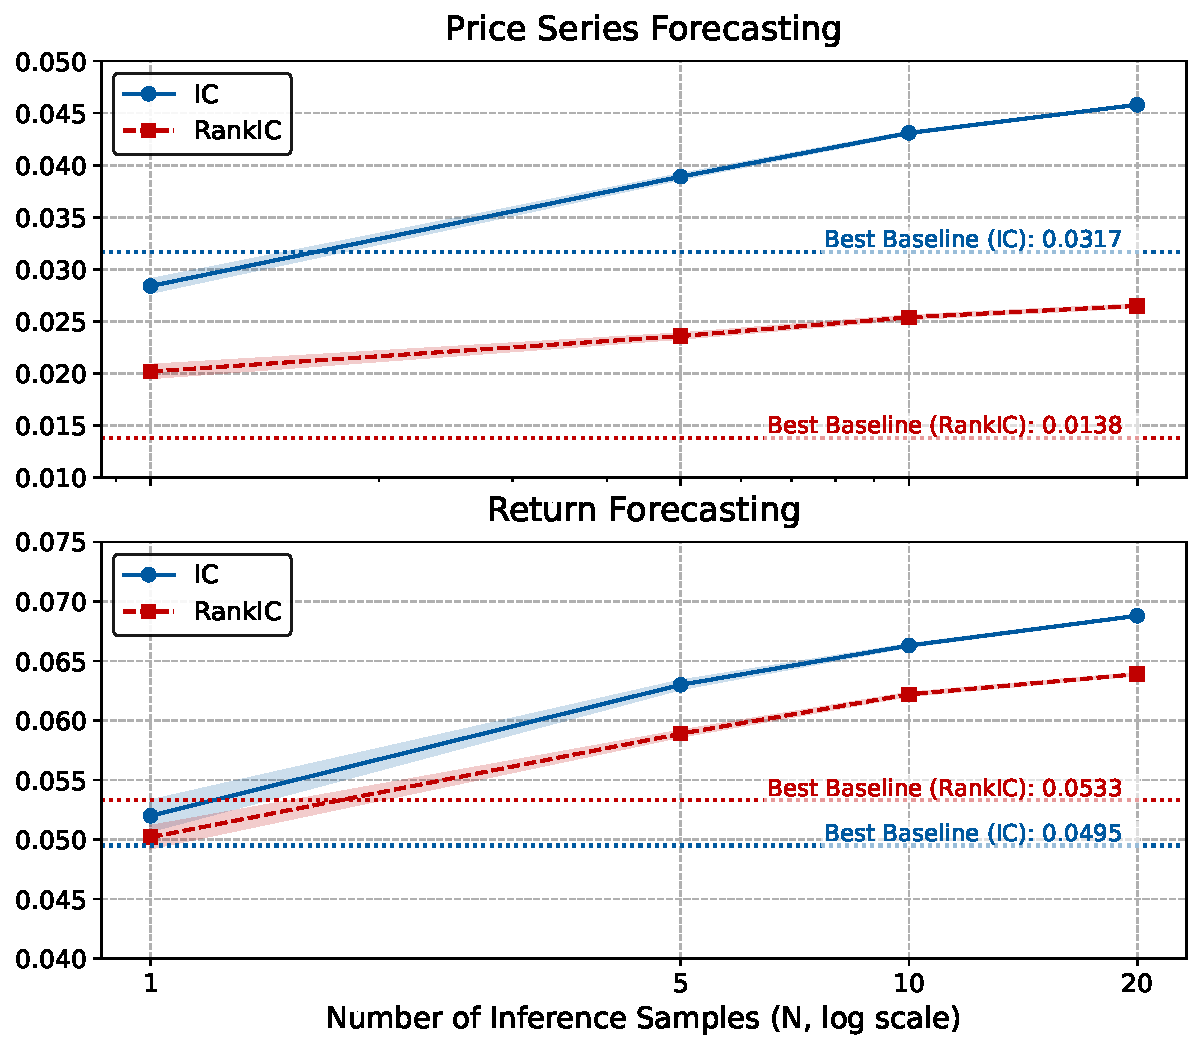
\includegraphics[width=1.0\columnwidth]{img/mc_sampling_performance.pdf}
    \caption{추론 샘플 수(N)가 예측 성능에 미치는 영향. 선은 서로 다른 무작위 시드를 사용한 5회 실행의 평균 성능을 나타내며, 음영 영역은 표준편차를 나타낸다.
    % 추론 샘플 크기(N)가 예측 성능에 미치는 영향. 평균(선)과 표준편차(음영)는 서로 다른 무작위 시드를 사용한 5회 실행에서 계산된다.
    }
    \label{fig:inference_sample}
\end{figure}

\subsection{테스트 시점 스케일링}
\label{sec:test_time_scaling}

우리의 확률적 생성 프레임워크의 주목할 만한 장점은 모델을 재학습하지 않고도 추론 시점에 예측 정확도를 향상시킬 수 있다는 점이다. 확률적 샘플링을 활용함으로써 Kronos는 동일한 맥락에서 여러 개의 서로 다른 미래 궤적을 생성할 수 있다. 우리는 샘플링된 경로 수를 늘려가며 그 결과를 평균함으로써 이러한 예측들을 앙상블하는 효과를 조사한다. 그림~\ref{fig:inference_sample}은 샘플 수의 함수로서 예측 과제 성능을 제시한다. 결과는 앙상블에 더 많은 샘플이 포함될수록 IC와 RankIC 모두에서 일관된 향상이 나타남을 보여준다. 여러 경로에 걸친 평균은 생성 과정에 내재한 확률성을 완화하고 예측 분산을 줄여, 더 견고하고 안정적인 추정치를 산출한다. 이 능력은 실무자가 추론 시 계산 비용과 원하는 예측 정확도 수준 사이의 균형을 맞출 수 있게 하는 절충점을 제공한다.


\section{Conclusion}

본 연구에서 우리는 금융 K-line 시퀀스를 위해 특별히 설계된 foundation model인 Kronos를 소개한다. Kronos는 새로운 2단계 프레임워크를 사용하며, 여기서 instance-based 토크나이저가 먼저 연속적인 시장 데이터를 계층적인 coarse-to-fine 토큰으로 이산화하고, 이어서 이를 대규모 자기회귀 Transformer가 모델링한다. 포괄적인 실증 평가는 Kronos가
가격 시계열 예측뿐만 아니라 합성 K-line 생성 및 변동성 예측과 같은 다른 관련 응용에서도 새로운 state-of-the-art 벤치마크를 수립하며, 기존 TSFMs와 기타 베이스라인을 크게 능가함을 보여준다. 이러한 결과는 Kronos를 정량 금융의 다양한 응용을 위한 견고하고 다재다능한 기반으로 자리매김시킨다.


% \bibliography{aaai2026}

\begin{thebibliography}{61}
\providecommand{\natexlab}[1]{#1}

\bibitem[{Achiam et~al.(2023)Achiam, Adler, Agarwal, Ahmad, Akkaya, Aleman,
  Almeida, Altenschmidt, Altman, Anadkat et~al.}]{achiam2023gpt}
Achiam, J.; Adler, S.; Agarwal, S.; Ahmad, L.; Akkaya, I.; Aleman, F.~L.;
  Almeida, D.; Altenschmidt, J.; Altman, S.; Anadkat, S.; et~al. 2023.
\newblock Gpt-4 technical report.
\newblock \emph{arXiv preprint arXiv:2303.08774}.

\bibitem[{Ansari et~al.(2024)Ansari, Stella, Turkmen, Zhang, Mercado, Shen,
  Shchur, Rangapuram, Arango, Kapoor et~al.}]{ansari2024chronos}
Ansari, A.~F.; Stella, L.; Turkmen, C.; Zhang, X.; Mercado, P.; Shen, H.;
  Shchur, O.; Rangapuram, S.~S.; Arango, S.~P.; Kapoor, S.; et~al. 2024.
\newblock Chronos: Learning the language of time series.
\newblock \emph{arXiv preprint arXiv:2403.07815}.

\bibitem[{Baidya and Lee(2024)}]{baidya2024addressing}
Baidya, R.; and Lee, S.-W. 2024.
\newblock Addressing the Non-Stationarity and Complexity of Time Series Data
  for Long-Term Forecasts.
\newblock \emph{Applied Sciences}, 14(11): 4436.

\bibitem[{Baker and Wurgler(2006)}]{baker2006investor}
Baker, M.; and Wurgler, J. 2006.
\newblock Investor sentiment and the cross-section of stock returns.
\newblock \emph{The journal of Finance}, 61(4): 1645--1680.

\bibitem[{Bollerslev(1986)}]{bollerslev1986generalized}
Bollerslev, T. 1986.
\newblock Generalized autoregressive conditional heteroskedasticity.
\newblock \emph{Journal of econometrics}, 31(3): 307--327.

\bibitem[{Brown et~al.(2020)Brown, Mann, Ryder, Subbiah, Kaplan, Dhariwal,
  Neelakantan, Shyam, Sastry, Askell et~al.}]{brown2020language}
Brown, T.; Mann, B.; Ryder, N.; Subbiah, M.; Kaplan, J.~D.; Dhariwal, P.;
  Neelakantan, A.; Shyam, P.; Sastry, G.; Askell, A.; et~al. 2020.
\newblock Language models are few-shot learners.
\newblock \emph{Advances in neural information processing systems}, 33:
  1877--1901.

\bibitem[{Brownlees and Gallo(2006)}]{brownlees2006financial}
Brownlees, C.~T.; and Gallo, G.~M. 2006.
\newblock Financial econometric analysis at ultra-high frequency: Data handling
  concerns.
\newblock \emph{Computational statistics \& data analysis}, 51(4): 2232--2245.

\bibitem[{Da, Engelberg, and Gao(2011)}]{da2011search}
Da, Z.; Engelberg, J.; and Gao, P. 2011.
\newblock In search of attention.
\newblock \emph{The journal of finance}, 66(5): 1461--1499.

\bibitem[{Das et~al.(2024)Das, Kong, Sen, and Zhou}]{das2024decoder}
Das, A.; Kong, W.; Sen, R.; and Zhou, Y. 2024.
\newblock A decoder-only foundation model for time-series forecasting.
\newblock In \emph{Forty-first International Conference on Machine Learning}.

\bibitem[{Desai et~al.(2021)Desai, Freeman, Wang, and
  Beaver}]{desai2021timevae}
Desai, A.; Freeman, C.; Wang, Z.; and Beaver, I. 2021.
\newblock Timevae: A variational auto-encoder for multivariate time series
  generation.
\newblock \emph{arXiv preprint arXiv:2111.08095}.

\bibitem[{Ding, Mittal, and Gopal(2025)}]{ding2025delphyne}
Ding, X.; Mittal, A.; and Gopal, A. 2025.
\newblock DELPHYNE: A Pre-Trained Model for General and Financial Time Series.
\newblock \emph{arXiv preprint arXiv:2506.06288}.

\bibitem[{Engle(1982)}]{engle1982autoregressive}
Engle, R.~F. 1982.
\newblock Autoregressive conditional heteroscedasticity with estimates of the
  variance of United Kingdom inflation.
\newblock \emph{Econometrica: Journal of the econometric society}, 987--1007.

\bibitem[{Flannery and Protopapadakis(2002)}]{flannery2002macroeconomic}
Flannery, M.~J.; and Protopapadakis, A.~A. 2002.
\newblock Macroeconomic factors do influence aggregate stock returns.
\newblock \emph{The review of financial studies}, 15(3): 751--782.

\bibitem[{Gao et~al.(2024)Gao, Koker, Queen, Hartvigsen, Tsiligkaridis, and
  Zitnik}]{gao2024units}
Gao, S.; Koker, T.; Queen, O.; Hartvigsen, T.; Tsiligkaridis, T.; and Zitnik,
  M. 2024.
\newblock Units: Building a unified time series model.
\newblock \emph{arXiv e-prints}, arXiv--2403.

\bibitem[{Garza, Challu, and Mergenthaler-Canseco(2023)}]{garza2023timegpt}
Garza, A.; Challu, C.; and Mergenthaler-Canseco, M. 2023.
\newblock TimeGPT-1.
\newblock \emph{arXiv preprint arXiv:2310.03589}.

\bibitem[{Goswami et~al.(2024)Goswami, Szafer, Choudhry, Cai, Li, and
  Dubrawski}]{goswami2024moment}
Goswami, M.; Szafer, K.; Choudhry, A.; Cai, Y.; Li, S.; and Dubrawski, A. 2024.
\newblock Moment: A family of open time-series foundation models.
\newblock \emph{arXiv preprint arXiv:2402.03885}.

\bibitem[{Holtzman et~al.(2019)Holtzman, Buys, Du, Forbes, and
  Choi}]{holtzman2019curious}
Holtzman, A.; Buys, J.; Du, L.; Forbes, M.; and Choi, Y. 2019.
\newblock The curious case of neural text degeneration.
\newblock \emph{arXiv preprint arXiv:1904.09751}.

\bibitem[{Kaplan et~al.(2020)Kaplan, McCandlish, Henighan, Brown, Chess, Child,
  Gray, Radford, Wu, and Amodei}]{kaplan2020scaling}
Kaplan, J.; McCandlish, S.; Henighan, T.; Brown, T.~B.; Chess, B.; Child, R.;
  Gray, S.; Radford, A.; Wu, J.; and Amodei, D. 2020.
\newblock Scaling laws for neural language models.
\newblock \emph{arXiv preprint arXiv:2001.08361}.

\bibitem[{Kim and Verrecchia(1991)}]{kim1991trading}
Kim, O.; and Verrecchia, R.~E. 1991.
\newblock Trading volume and price reactions to public announcements.
\newblock \emph{Journal of accounting research}, 29(2): 302--321.

\bibitem[{Kirillov et~al.(2023)Kirillov, Mintun, Ravi, Mao, Rolland, Gustafson,
  Xiao, Whitehead, Berg, Lo et~al.}]{kirillov2023segment}
Kirillov, A.; Mintun, E.; Ravi, N.; Mao, H.; Rolland, C.; Gustafson, L.; Xiao,
  T.; Whitehead, S.; Berg, A.~C.; Lo, W.-Y.; et~al. 2023.
\newblock Segment anything.
\newblock In \emph{Proceedings of the IEEE/CVF international conference on
  computer vision}, 4015--4026.

\bibitem[{Kohli and Kohers(1992)}]{kohli1992week}
Kohli, R.~K.; and Kohers, T. 1992.
\newblock The week-of-the-month effect in stock returns: The evidence from the
  S\&P composite index.
\newblock \emph{Journal of economics and finance}, 16(2): 129--137.

\bibitem[{Li et~al.(2024)Li, Liu, Liu, Fang, Wang, Xu, and Bian}]{li2024mars}
Li, J.; Liu, Y.; Liu, W.; Fang, S.; Wang, L.; Xu, C.; and Bian, J. 2024.
\newblock MarS: a Financial Market Simulation Engine Powered by Generative
  Foundation Model.
\newblock \emph{arXiv preprint arXiv:2409.07486}.

\bibitem[{Liu et~al.(2023)Liu, Hu, Zhang, Wu, Wang, Ma, and
  Long}]{liuitransformer}
Liu, Y.; Hu, T.; Zhang, H.; Wu, H.; Wang, S.; Ma, L.; and Long, M. 2023.
\newblock itransformer: Inverted transformers are effective for time series
  forecasting.
\newblock \emph{arXiv preprint arXiv:2310.06625}.

\bibitem[{Liu et~al.(2025)Liu, Qin, Shi, Chen, Yang, Huang, Wang, and
  Long}]{liu2025sundial}
Liu, Y.; Qin, G.; Shi, Z.; Chen, Z.; Yang, C.; Huang, X.; Wang, J.; and Long,
  M. 2025.
\newblock Sundial: A Family of Highly Capable Time Series Foundation Models.
\newblock \emph{arXiv preprint arXiv:2502.00816}.

\bibitem[{Liu et~al.(2022)Liu, Wu, Wang, and Long}]{liu2022non}
Liu, Y.; Wu, H.; Wang, J.; and Long, M. 2022.
\newblock Non-stationary transformers: Exploring the stationarity in time
  series forecasting.
\newblock \emph{Advances in neural information processing systems}, 35:
  9881--9893.

\bibitem[{Liu et~al.(2024)Liu, Zhang, Li, Huang, Wang, and Long}]{liu2024timer}
Liu, Y.; Zhang, H.; Li, C.; Huang, X.; Wang, J.; and Long, M. 2024.
\newblock Timer: Generative pre-trained transformers are large time series
  models.
\newblock \emph{arXiv preprint arXiv:2402.02368}.

\bibitem[{Loshchilov and Hutter(2017)}]{loshchilov2017decoupled}
Loshchilov, I.; and Hutter, F. 2017.
\newblock Decoupled weight decay regularization.
\newblock \emph{arXiv preprint arXiv:1711.05101}.

\bibitem[{Mandelbrot et~al.(1963)}]{mandelbrot1963variation}
Mandelbrot, B.; et~al. 1963.
\newblock The variation of certain speculative prices.
\newblock \emph{Journal of business}, 36(4): 394.

\bibitem[{McKibbin, Noland, and Shuetrim(2025)}]{mckibbin2025global}
McKibbin, W.; Noland, M.; and Shuetrim, G. 2025.
\newblock The global economic effects of Trump's 2025 tariffs.
\newblock Technical report, Peterson Institute for International Economics.

\bibitem[{Nie et~al.(2022)Nie, Nguyen, Sinthong, and Kalagnanam}]{nie2022time}
Nie, Y.; Nguyen, N.~H.; Sinthong, P.; and Kalagnanam, J. 2022.
\newblock A time series is worth 64 words: Long-term forecasting with
  transformers.
\newblock \emph{arXiv preprint arXiv:2211.14730}.

\bibitem[{Nison(2001)}]{nison2001japanese}
Nison, S. 2001.
\newblock \emph{Japanese candlestick charting techniques: a contemporary guide
  to the ancient investment techniques of the Far East}.
\newblock Penguin.

\bibitem[{Ozenbas et~al.(2008)}]{ozenbas2008intra}
Ozenbas, D.; et~al. 2008.
\newblock Intra-day trading volume patterns of equity markets: A study of US
  and European stock markets.
\newblock \emph{International Business \& Economics Research Journal (IBER)},
  7(8).

\bibitem[{Podobnik et~al.(2009)Podobnik, Horvatic, Petersen, and
  Stanley}]{podobnik2009cross}
Podobnik, B.; Horvatic, D.; Petersen, A.~M.; and Stanley, H.~E. 2009.
\newblock Cross-correlations between volume change and price change.
\newblock \emph{Proceedings of the National Academy of Sciences}, 106(52):
  22079--22084.

\bibitem[{Rabanser et~al.(2020)Rabanser, Januschowski, Flunkert, Salinas, and
  Gasthaus}]{rabanser2020effectiveness}
Rabanser, S.; Januschowski, T.; Flunkert, V.; Salinas, D.; and Gasthaus, J.
  2020.
\newblock The effectiveness of discretization in forecasting: An empirical
  study on neural time series models.
\newblock \emph{arXiv preprint arXiv:2005.10111}.

\bibitem[{Radford et~al.(2021)Radford, Kim, Hallacy, Ramesh, Goh, Agarwal,
  Sastry, Askell, Mishkin, Clark et~al.}]{radford2021learning}
Radford, A.; Kim, J.~W.; Hallacy, C.; Ramesh, A.; Goh, G.; Agarwal, S.; Sastry,
  G.; Askell, A.; Mishkin, P.; Clark, J.; et~al. 2021.
\newblock Learning transferable visual models from natural language
  supervision.
\newblock In \emph{International conference on machine learning}, 8748--8763.
  PmLR.

\bibitem[{Rasul et~al.(2023)Rasul, Ashok, Williams, Khorasani, Adamopoulos,
  Bhagwatkar, Bilo{\v{s}}, Ghonia, Hassen, Schneider et~al.}]{rasul2023lag}
Rasul, K.; Ashok, A.; Williams, A.~R.; Khorasani, A.; Adamopoulos, G.;
  Bhagwatkar, R.; Bilo{\v{s}}, M.; Ghonia, H.; Hassen, N.; Schneider, A.;
  et~al. 2023.
\newblock Lag-llama: Towards foundation models for time series forecasting.
\newblock In \emph{R0-FoMo: Robustness of Few-shot and Zero-shot Learning in
  Large Foundation Models}.

\bibitem[{Shi et~al.(2025)Shi, Luo, Ge, Yang, Shan, and
  Wang}]{shi2025scalableimagetokenizationindex}
Shi, F.; Luo, Z.; Ge, Y.; Yang, Y.; Shan, Y.; and Wang, L. 2025.
\newblock Scalable Image Tokenization with Index Backpropagation Quantization.
\newblock arXiv:2412.02692.

\bibitem[{Su et~al.(2024)Su, Ahmed, Lu, Pan, Bo, and Liu}]{su2024roformer}
Su, J.; Ahmed, M.; Lu, Y.; Pan, S.; Bo, W.; and Liu, Y. 2024.
\newblock Roformer: Enhanced transformer with rotary position embedding.
\newblock \emph{Neurocomputing}, 568: 127063.

\bibitem[{Talukder, Yue, and Gkioxari(2024)}]{talukder2024totem}
Talukder, S.; Yue, Y.; and Gkioxari, G. 2024.
\newblock Totem: Tokenized time series embeddings for general time series
  analysis.
\newblock \emph{arXiv preprint arXiv:2402.16412}.

\bibitem[{Van Den~Oord, Vinyals et~al.(2017)}]{van2017neural}
Van Den~Oord, A.; Vinyals, O.; et~al. 2017.
\newblock Neural discrete representation learning.
\newblock \emph{Advances in neural information processing systems}, 30.

\bibitem[{Wang et~al.(2024{\natexlab{a}})Wang, Wu, Shi, Hu, Luo, Ma, Zhang, and
  Zhou}]{wang2024timemixer}
Wang, S.; Wu, H.; Shi, X.; Hu, T.; Luo, H.; Ma, L.; Zhang, J.~Y.; and Zhou, J.
  2024{\natexlab{a}}.
\newblock Timemixer: Decomposable multiscale mixing for time series
  forecasting.
\newblock \emph{arXiv preprint arXiv:2405.14616}.

\bibitem[{Wang et~al.(2025)Wang, Lin, Teng, Zhu, Ren, Feng, and
  Liu}]{wang2025bridging}
Wang, Y.; Lin, Z.; Teng, Y.; Zhu, Y.; Ren, S.; Feng, J.; and Liu, X. 2025.
\newblock Bridging continuous and discrete tokens for autoregressive visual
  generation.
\newblock \emph{arXiv preprint arXiv:2503.16430}.

\bibitem[{Wang et~al.(2024{\natexlab{b}})Wang, Wu, Dong, Liu, Long, and
  Wang}]{wang2024deep}
Wang, Y.; Wu, H.; Dong, J.; Liu, Y.; Long, M.; and Wang, J. 2024{\natexlab{b}}.
\newblock Deep time series models: A comprehensive survey and benchmark.
\newblock \emph{arXiv preprint arXiv:2407.13278}.

\bibitem[{Wang et~al.(2024{\natexlab{c}})Wang, Wu, Dong, Qin, Zhang, Liu, Qiu,
  Wang, and Long}]{wang2024timexer}
Wang, Y.; Wu, H.; Dong, J.; Qin, G.; Zhang, H.; Liu, Y.; Qiu, Y.; Wang, J.; and
  Long, M. 2024{\natexlab{c}}.
\newblock Timexer: Empowering transformers for time series forecasting with
  exogenous variables.
\newblock \emph{arXiv preprint arXiv:2402.19072}.

\bibitem[{Wheeler and Varner(2024)}]{wheeler2024marketgpt}
Wheeler, A.; and Varner, J.~D. 2024.
\newblock MarketGPT: Developing a Pre-trained transformer (GPT) for Modeling
  Financial Time Series.
\newblock \emph{arXiv preprint arXiv:2411.16585}.

\bibitem[{Woo et~al.(2024)Woo, Liu, Kumar, Xiong, Savarese, and
  Sahoo}]{woo2024unified}
Woo, G.; Liu, C.; Kumar, A.; Xiong, C.; Savarese, S.; and Sahoo, D. 2024.
\newblock Unified Training of Universal Time Series Forecasting Transformers.
\newblock In \emph{International Conference on Machine Learning}, 53140--53164.
  PMLR.

\bibitem[{Wu et~al.(2022)Wu, Hu, Liu, Zhou, Wang, and Long}]{wu2022timesnet}
Wu, H.; Hu, T.; Liu, Y.; Zhou, H.; Wang, J.; and Long, M. 2022.
\newblock Timesnet: Temporal 2d-variation modeling for general time series
  analysis.
\newblock \emph{arXiv preprint arXiv:2210.02186}.

\bibitem[{Xiaoming et~al.(2025)Xiaoming, Shiyu, Yuqi, Dianqi, Zhou, Qingsong,
  and Jin}]{xiaoming2025time}
Xiaoming, S.; Shiyu, W.; Yuqi, N.; Dianqi, L.; Zhou, Y.; Qingsong, W.; and Jin,
  M. 2025.
\newblock Time-MoE: Billion-Scale Time Series Foundation Models with Mixture of
  Experts.
\newblock In \emph{ICLR 2025: The Thirteenth International Conference on
  Learning Representations}. International Conference on Learning
  Representations.

\bibitem[{Xiong et~al.(2020)Xiong, Yang, He, Zheng, Zheng, Xing, Zhang, Lan,
  Wang, and Liu}]{xiong2020layer}
Xiong, R.; Yang, Y.; He, D.; Zheng, K.; Zheng, S.; Xing, C.; Zhang, H.; Lan,
  Y.; Wang, L.; and Liu, T. 2020.
\newblock On layer normalization in the transformer architecture.
\newblock In \emph{International conference on machine learning}, 10524--10533.
  PMLR.

\bibitem[{Xu et~al.(2024)Xu, Liu, Hao, Li, Meng, and Zhang}]{xu2024plutus}
Xu, Y.; Liu, A.; Hao, J.; Li, Z.; Meng, S.; and Zhang, G. 2024.
\newblock PLUTUS: A Well Pre-trained Large Unified Transformer can Unveil
  Financial Time Series Regularities.
\newblock \emph{arXiv preprint arXiv:2408.10111}.

\bibitem[{Yang et~al.(2020)Yang, Liu, Zhou, Bian, and Liu}]{yang2020qlib}
Yang, X.; Liu, W.; Zhou, D.; Bian, J.; and Liu, T.-Y. 2020.
\newblock Qlib: An ai-oriented quantitative investment platform.
\newblock \emph{arXiv preprint arXiv:2009.11189}.

\bibitem[{Yao et~al.(2024)Yao, Yang, Jiang, Liang, Jin, and
  Pan}]{yao2024towards}
Yao, Q.; Yang, C.-H.~H.; Jiang, R.; Liang, Y.; Jin, M.; and Pan, S. 2024.
\newblock Towards Neural Scaling Laws for Time Series Foundation Models.
\newblock \emph{arXiv preprint arXiv:2410.12360}.

\bibitem[{Yoon, Jarrett, and Van~der Schaar(2019)}]{yoon2019time}
Yoon, J.; Jarrett, D.; and Van~der Schaar, M. 2019.
\newblock Time-series generative adversarial networks.
\newblock \emph{Advances in neural information processing systems}, 32.

\bibitem[{Yu et~al.(2023)Yu, Lezama, Gundavarapu, Versari, Sohn, Minnen, Cheng,
  Birodkar, Gupta, Gu et~al.}]{yu2023language}
Yu, L.; Lezama, J.; Gundavarapu, N.~B.; Versari, L.; Sohn, K.; Minnen, D.;
  Cheng, Y.; Birodkar, V.; Gupta, A.; Gu, X.; et~al. 2023.
\newblock Language Model Beats Diffusion--Tokenizer is Key to Visual
  Generation.
\newblock \emph{arXiv preprint arXiv:2310.05737}.

\bibitem[{Yuan and Qiao(2024)}]{yuan2024diffusion}
Yuan, X.; and Qiao, Y. 2024.
\newblock Diffusion-ts: Interpretable diffusion for general time series
  generation.
\newblock \emph{arXiv preprint arXiv:2403.01742}.

\bibitem[{Zeng et~al.(2023)Zeng, Chen, Zhang, and Xu}]{zeng2023transformers}
Zeng, A.; Chen, M.; Zhang, L.; and Xu, Q. 2023.
\newblock Are transformers effective for time series forecasting?
\newblock In \emph{Proceedings of the AAAI conference on artificial
  intelligence}, 9, 11121--11128.

\bibitem[{Zhang and Sennrich(2019)}]{zhang2019root}
Zhang, B.; and Sennrich, R. 2019.
\newblock Root mean square layer normalization.
\newblock \emph{Advances in Neural Information Processing Systems}, 32.

\bibitem[{Zhang and Hua(2025)}]{zhang2025major}
Zhang, L.; and Hua, L. 2025.
\newblock Major Issues in High-Frequency Financial Data Analysis: A Survey of
  Solutions.
\newblock \emph{Mathematics}, 13(3): 347.

\bibitem[{Zhao, Xiong, and Kr{\"a}henb{\"u}hl(2024)}]{zhao2024image}
Zhao, Y.; Xiong, Y.; and Kr{\"a}henb{\"u}hl, P. 2024.
\newblock Image and video tokenization with binary spherical quantization.
\newblock \emph{arXiv preprint arXiv:2406.07548}.

\bibitem[{Zhou et~al.(2022)Zhou, Ma, Wen, Wang, Sun, and
  Jin}]{zhou2022fedformer}
Zhou, T.; Ma, Z.; Wen, Q.; Wang, X.; Sun, L.; and Jin, R. 2022.
\newblock Fedformer: Frequency enhanced decomposed transformer for long-term
  series forecasting.
\newblock In \emph{International conference on machine learning}, 27268--27286.
  PMLR.

\bibitem[{Zhu et~al.(2024)Zhu, Li, Xin, and Xu}]{zhu2024addressing}
Zhu, Y.; Li, B.; Xin, Y.; and Xu, L. 2024.
\newblock Addressing representation collapse in vector quantized models with
  one linear layer.
\newblock \emph{arXiv preprint arXiv:2411.02038}.

\end{thebibliography}

\clearpage
\appendix

\setcounter{secnumdepth}{1}


\section*{부록 개요}

이 부록은 본 논문을 뒷받침하는 보충 자료를 제공한다. 데이터 전처리 파이프라인, 모델 및 학습 설정, 모든 과제의 실험 설정을 자세히 설명하고, 하이퍼파라미터 민감도 분석, 전체 결과 표, 예측 사례를 포함한 추가 결과를 제시한다.

\section{관련 연구}

\subsection{시계열 토큰화}

The recent success of large, token-based models has spurred a growing interest in discretizing continuous time series. This tokenization process is pivotal for adapting such architectures for time series analysis, yet dedicated research in this area remains sparse. Early efforts like Chronos~\cite{ansari2024chronos} employ scaling and uniform quantization, while TOTEM~\cite{talukder2024totem} utilizes a Vector Quantized Variational Autoencoder (VQ-VAE)~\cite{van2017neural}—a seminal approach that maps encoder outputs to learned discrete latent codes—for codebook-based tokenization. Given this nascent landscape, we draw inspiration from the more mature field of visual tokenization. Beyond the foundational VQ-VAE, innovations include Lookup-Free Quantization (LFQ)~\cite{yu2023language}, achieving high-fidelity reconstruction via an implicit codebook without explicit lookups. Binary Spherical Quantization (BSQ)~\cite{zhao2024image} advances implicit codebooks using spherical projection for an exponentially growing vocabulary, offering bounded quantization error and improved trainability over LFQ. Further, Index Backpropagation Quantization (IBQ)~\cite{shi2025scalableimagetokenizationindex} tackles codebook collapse by making all code entries differentiable, enabling stable joint optimization of large-scale codebooks and the visual encoder. While primarily designed for visual data, these methods can also be applied to discretize general multivariate time series.

\subsection{범용 시계열 파운데이션 모델}

The paradigm of time series analysis has recently been reshaped by Time Series Foundation Models (TSFMs), drawing inspiration from the success of Large Language Models in leveraging massive pre-trained Transformers. These models are trained on vast, multi-domain corpora—some with over a hundred billion data points—to achieve remarkable zero-shot or few-shot performance on general forecasting benchmarks. This versatility is enabled by diverse architectures, including decoder-only models like Lag-Llama~\cite{rasul2023lag}, TimesFM~\cite{das2024decoder}, Timer~\cite{liu2024timer}, Time-MoE~\cite{xiaoming2025time}, and Sumdial~\cite{liu2025sundial}; encoder-only frameworks like MOMENT~\cite{goswami2024moment} and Moirai~\cite{woo2024unified}; encoder-decoder structures such as TimeGPT~\cite{garza2023timegpt}; and models with modified Transformer blocks for multi-task learning like UniTS~\cite{gao2024units}. At the input level, they employ generic representations such as direct value patching (e.g., TimesFM~\cite{das2024decoder}, MOMENT~\cite{goswami2024moment}), value quantization into a fixed vocabulary (e.g., Chronos~\cite{ansari2024chronos}), or treating consecutive time points as tokens (e.g., Timer~\cite{liu2024timer}). Several of these models also extend to probabilistic forecasting (e.g., Lag-Llama~\cite{rasul2023lag}, Moirai~\cite{woo2024unified}, Chronos~\cite{ansari2024chronos} and Sumdial~\cite{liu2025sundial}).

However, the very generality that drives their success on broad benchmarks becomes a limitation in specialized domains. To provide a concrete comparison, we summarize key attributes of prominent TSFMs in Table~\ref{tab:tsfm_comparison}. A important observation from the table is the minuscule proportion of financial data within the pre-training corpora of these general-purpose models, with most dedicating less than 1\% of their data to this domain. This data imbalance means that the unique structural properties, non-stationarity, and complex dynamics of financial K-line sequences are largely overlooked or averaged out during pre-training, often resulting in suboptimal performance for financial tasks. To address this fundamental gap in pre-training, we introduce Kronos, a foundation model built from the ground up on a massive corpus composed exclusively of financial K-line data.

\subsection{금융 시계열 파운데이션 모델}

The development of foundation models specifically for finance time series is a nascent but rapidly growing field. These efforts can be divided into two main streams. The first focuses on general financial time series, including K-line data. For instance, PLUTUS~\cite{xu2024plutus} introduces an invertible embedding and multi-scale temporal attention, pre-trained on massive datasets to uncover market regularities. DELPHYNE~\cite{ding2025delphyne} is designed explicitly to counteract the negative transfer from non-financial data. While promising, neither of these works has released their code or models, precluding direct empirical comparison. The second stream targets order flow data, where models like MarketGPT~\cite{wheeler2024marketgpt} and MarS~\cite{li2024mars} act as generative engines for realistic market simulation. These pioneering efforts validate the value of domain-specific pre-training. However, K-line data possesses broader applicability than order flow, as it is readily available across all markets and suitable for diverse time horizons where order flow data is often inaccessible. Despite its central importance, a versatile and open-source foundation model for K-line analysis remains a notable gap. We introduce Kronos to fill this void, offering a unified, scalable framework designed specifically for financial K-line data.

\begin{table*}[t]
\centering

\resizebox{\textwidth}{!}{%
\begin{tabular}{@{}lllccl@{}}
\toprule
\textbf{Model} & \textbf{아키텍처} & \textbf{토큰화} & \textbf{확률적} & \textbf{금융 데이터 비율(추정)} & \textbf{주요 도메인} \\ \midrule
\textbf{Kronos (Ours)} & \textbf{Decoder-only} & \textbf{Discrete (BSQ)} & \textbf{Yes} & \textbf{100\%} & \textbf{Financial K-lines} \\
\midrule
Sundial~\cite{liu2025sundial} & Decoder-only & Continuous & Yes & 1.02\% & General \\
Time-MoE~\cite{xiaoming2025time} & Decoder-only & Continuous & No & $<$0.01\% & General \\
Moirai~\cite{woo2024unified} & Encoder-only & Continuous & Yes & 0.10\% & General \\
MOMENT~\cite{goswami2024moment} & Encoder-only & Continuous & No & 1.60\% & General \\
Chronos~\cite{ansari2024chronos} & Encoder-Decoder & Discrete (Quantization) & Yes & 0.45\% & General \\
Timer~\cite{liu2024timer} & Decoder-only & Continuous & No & 0.03\% & General \\
TimesFM~\cite{das2024decoder} & Decoder-only & Continuous & No & $<$0.01\% & General \\
UniTS~\cite{gao2024units} & Encoder-only & Continuous & No & Unknown & General \\
Lag-Llama~\cite{rasul2023lag} & Decoder-only & Continuous & Yes & 0.01\% & General \\
% TimeGPT~\cite{garza2023timegpt} & Encoder-Decoder & Continuous & No & Unknown & General \\
\bottomrule
\end{tabular}%
}
\caption{시계열 파운데이션 모델 비교. 이 표는 아키텍처 선택, 토큰화 방법, 확률적 예측 기능, 그리고 사전학습 말뭉치에서 금융 데이터가 차지하는 추정 비율을 강조한다.}
\label{tab:tsfm_comparison}
\end{table*}

\section{데이터셋 세부 사항}
\label{sec:dataset_details}

\begin{table}[t]
\centering
\small

\setlength{\tabcolsep}{4pt} % Reduce space between columns
\resizebox{\columnwidth}{!}{%
\begin{tabular}{l c c cc}
\toprule
& & & \multicolumn{2}{c}{\textbf{Max. Consecutive Bars}} \\
\cmidrule(lr){4-5}
\textbf{주기} & \textbf{\begin{tabular}[c]{@{}c@{}}Min. Length \\ (bars)\end{tabular}} & \textbf{\begin{tabular}[c]{@{}c@{}}Price Jump \\ Threshold\end{tabular}} & \textbf{비유동} & \textbf{정체} \\
\midrule
1min    & 2048 & 0.10 & 15 & 45 \\
5min    & 1024 & 0.15 & 3 & 10 \\
10min   & 512  & 0.15 & 3 & 6  \\
15min   & 512  & 0.15 & 2 & 5  \\
20min   & 512  & 0.15 & 2 & 5  \\
30min   & 512  & 0.20 & 2 & 3  \\
40min   & 256  & 0.20 & 1 & 3  \\
60min   & 256  & 0.20 & 1 & 3  \\
2H      & 128  & 0.25 & 1 & 3  \\
4H      & 128  & 0.25 & 1 & 3  \\
Daily   & 128  & 0.30 & 1 & 3  \\
Weekly  & 16   & 0.50 & 0 & 2  \\
\bottomrule
\end{tabular}}
\caption{저품질 데이터 필터링 파이프라인의 주기별 파라미터. 임계값은 서로 다른 시간 주기의 고유한 동학을 반영하도록 조정된다.}
\label{tab:cleaning_parameters}
\end{table}

\subsection{데이터 전처리와 정제}
\label{appendix:data_cleaning}

This section details the preprocessing and cleaning pipeline applied to the large-scale K-line dataset used for pre-training. The dataset is aggregated from over 40 exchanges across more than 30 countries, comprising a diverse range of asset classes at multiple temporal frequencies (1-minute to weekly). A statistical overview is provided in Table~\ref{tab:dataset_overview}. The integrity of large-scale pre-training is contingent upon high-quality input data. Raw K-line series, however, are frequently contaminated by artifacts stemming from low liquidity, price limits, or data feed errors. To mitigate the impact of such issues, we implement a rigorous, two-stage pipeline designed to process missing values and filter out low-quality data segments.

\begin{algorithm}[t]
\caption{저품질 구간 필터링 파이프라인}
\label{alg:segment_filtering}
\begin{algorithmic}[1]
\Statex \textbf{입력:} Raw K-line series $S_{raw}$, Parameter set $\Theta$ for a given frequency (from Table~\ref{tab:cleaning_parameters})
\Statex \textbf{출력:} A set of clean K-line segments $\mathcal{C}$

\Function{FilterLowQualitySegments}{$S_{raw}, \Theta$}
    \State $\mathcal{C} \leftarrow \emptyset$ \Comment{Initialize the set of final clean segments}
    \State $\mathcal{S}_{initial} \leftarrow \text{PartitionByPriceJumps}(S_{raw}, \Theta_{\text{jump}})$ \Comment{Split by structural breaks}

    \ForAll{segment $S$ in $\mathcal{S}_{initial}$}
        \State $M_{illiquid} \leftarrow \text{FlagConsecutiveIlliquid}(S, \Theta_{\text{illiquid}})$ \Comment{Identify illiquid periods}
        \State $M_{stagnant} \leftarrow \text{FlagConsecutiveStagnant}(S, \Theta_{\text{stagnant}})$ \Comment{Identify stagnant periods}
        \State $M_{invalid} \leftarrow M_{illiquid} \lor M_{stagnant}$ \Comment{Combine masks for all invalid points}

        \State $\mathcal{S}_{clean} \leftarrow \text{ExtractValidSubsequences}(S, M_{invalid})$ \Comment{Split segment on invalid boundaries}

        \ForAll{subsequence $S_{sub}$ in $\mathcal{S}_{clean}$}
            \If{$\text{Length}(S_{sub}) \ge \Theta_{\text{min\_len}}$}
                \State $\mathcal{C} \leftarrow \mathcal{C} \cup \{S_{sub}\}$ \Comment{Add valid, sufficiently long segment}
            \EndIf
        \EndFor
    \EndFor

    \State \textbf{return} $\mathcal{C}$
\EndFunction
\end{algorithmic}
\end{algorithm}

\subsubsection{결측값 처리}
We employ a field-specific strategy to handle missing values, which are typically represented as `NaN' (Not a Number) or `Inf' (Infinity).

\begin{itemize}
    \item \textbf{Price Fields (Open, High, Low, Close):} For price-related fields, we treat missing values as hard boundaries. Inspired by TimeMOE~\cite{xiaoming2025time}, we partition the time series into contiguous, valid sub-sequences at each occurrence of a missing price value. This approach ensures that each resulting segment maintains its internal temporal integrity without unwarranted imputation.
    \item \textbf{Volume and Amount Fields:} In contrast, for volume and amount fields, which primarily serve as auxiliary covariates, we impute missing values with zero. To enhance model robustness to sparse or unavailable volumetric data, we introduce a regularization technique: during training, both volume and amount are randomly set to zero for 5\% of the input samples. This encourages the model to learn to make effective predictions from price information alone.
\end{itemize}

\subsubsection{저품질 구간 필터링}
Beyond addressing discrete missing values, our pipeline systematically identifies and removes entire segments of low-quality data. This is achieved through a multi-stage filtering process where tolerance thresholds are dynamically adjusted according to the data's temporal frequency, as detailed in Table~\ref{tab:cleaning_parameters}. The procedure, formalized in Algorithm~\ref{alg:segment_filtering}, consists of the following steps:

\begin{itemize}
    \item \textbf{Structural Break Segmentation.} The initial filtering stage partitions the series based on significant price discontinuities. We identify these breaks by calculating the relative price jump between the previous bar's close and the current bar's open ($| \text{open}_t / \text{close}_{t-1} - 1 |$). If this jump exceeds a frequency-specific threshold, the sequence is split. This step effectively isolates artifacts arising from events such as contract rollovers, stock splits, or dividend distributions.
    \item \textbf{Filtering of Illiquid Periods.} Within each segment from the previous step, we screen for periods of sustained illiquidity. A bar is deemed illiquid if its trading volume is zero or near-zero. If the number of consecutive illiquid bars exceeds a frequency-dependent threshold, the corresponding period is flagged as invalid.
    \item \textbf{Filtering of Price Stagnation.} We apply a similar method to filter periods of price stagnation, where the closing price remains constant over an extended duration. This often indicates potential data feed issues or market inactivity. If the length of a stagnant streak surpasses its frequency-specific tolerance, it is also flagged as an invalid period.
    \item \textbf{Final Segment Validation.} After flagging all illiquid and stagnant periods, the initial segments are further split at the boundaries of these flagged regions. Finally, only the resulting sub-segments that meet the frequency-specific minimum length requirement ($\Theta_{\text{min\_len}}$ in Table~\ref{tab:cleaning_parameters}) are retained for the final pre-training dataset. This ensures each sample is sufficiently long to support meaningful model learning.
\end{itemize}

\section{구현 세부 사항}
\label{sec:implementation_details}

In this section, we provide further details on the implementation of Kronos, covering data preprocessing, model architecture, and configurations for training and inference.

\subsection{입력 전처리}
\label{sec:input_processing}
Each input K-line sequence $\mathbf{x} = (\mathbf{x}_1, \mathbf{x}_2, \dots, \mathbf{x}_T)$, where $\mathbf{x}_t \in \mathbb{R}^D$, is normalized in a two-step procedure before being passed to the tokenizer. First, we apply z-score normalization independently to each of the $D$ feature dimensions (e.g., Open, High, Low, Close, Volume and Amount). Second, to mitigate the potential impact of extreme outliers on training stability, the normalized values are clipped to the range $[-5, 5]$. This process ensures that all input features have a consistent scale while preserving the model's robustness against anomalous data points.

\begin{table*}[t!]
  \centering

  \resizebox{0.9\textwidth}{!}{%
  \begin{tabular}{@{}lcccccc@{}}
    \toprule
    \textbf{Model} & \textbf{FFN Dropout} & \textbf{Residual Dropout} & \textbf{Attention Dropout} & \textbf{Token Dropout} & \textbf{Learning Rate} & \textbf{Weight Decay} \\
    \midrule
    $\text{Kronos}_{small}$ & 0.25 & 0.25 & 0.1 & 0.1 & \num{1e-3} & 0.01 \\
    $\text{Kronos}_{base}$  & 0.20 & 0.20 & 0.0 & 0.0 & \num{5e-4} & 0.05 \\
    $\text{Kronos}_{large}$ & 0.00 & 0.00 & 0.0 & 0.0 & \num{2e-4} & 0.10 \\
    \bottomrule
  \end{tabular}%
  }
  \caption{Kronos 모델 계열의 하이퍼파라미터 설정. 모든 모델은 AdamW 옵티마이저로 학습된다.}
  \label{tab:training_params}
\end{table*}

\subsection{모델 아키텍처}

\paragraph{시간 임베딩.} To capture cyclical patterns inherent in financial markets, such as intraday, weekly, and monthly seasonality~\cite{ozenbas2008intra,kohli1992week}, we incorporate learnable temporal embeddings. We extract five time-related features for each K-line entry: minute-of-day, hour-of-day, day-of-week, day-of-month, and month-of-year. Each feature is mapped to a dense vector via a dedicated embedding layer. These temporal embeddings are summed and then added to the input representation of each corresponding token, providing the model with explicit temporal context.

\paragraph{K-line 토큰화.} The tokenizer's autoencoder is designed to be lightweight. The encoder and decoder each consist of 3 Transformer layers, with a model dimension of 256, a feed-forward network dimension of 512, and 4 attention heads. Following the official open-source implementation of BSQ\footnote{\url{https://github.com/zhaoyue-zephyrus/bsq-vit}}, we configure the key quantization hyperparameters as follows: a commitment weight $\beta=0.05$, entropy penalty weights $\gamma_0=1.0$ and $\gamma=1.1$, and an overall entropy scale $\zeta=0.05$. The balancing hyperparameter $\lambda$ for the quantization loss in our objective is set to 1. The quantization group size is set to 5 for tractable entropy computation.

\paragraph{Transformer 블록 아키텍처.} To encode the sequential nature of the data, we employ causal self-attention with Rotary Position Embeddings (RoPE)~\cite{su2024roformer}, which injects relative positional information. The attention operation is formulated as follows:
\begin{equation}
    \text{Attention}(Q, K, V) = \text{CausalMask}\left(\frac{Q' (K')^T}{\sqrt{d_k}}\right)V
\end{equation}
where $d_k$ is the dimension of the key vectors, and $\text{CausalMask}$ prevents attending to future positions. The matrices $Q'$ and $K'$ represent the original query and key matrices with RoPE transformations applied. Furthermore, we adopt the Pre-Layer Normalization (Pre-LN)~\cite{xiong2020layer} to improve training stability, specifically utilizing Root Mean Square Layer Normalization (RMSNorm)~\cite{zhang2019root} for its computational efficiency and performance.

\subsection{학습 설정}
The training hyperparameters are carefully selected for each model size to ensure a stable pre-training process. As model scale increases, we decrease the peak learning rate and dropout probability while increasing the weight decay. We employ the AdamW optimizer~\cite{loshchilov2017decoupled} and a cosine learning rate schedule with a linear warm-up phase. The learning rate warms up from 10\% of its peak value over the first 15,000 training steps. Table~\ref{tab:training_params} details the specific hyperparameter settings for each model variant.

\begin{table*}[t!]
\centering
\setlength{\tabcolsep}{4pt}

\begin{tabular}{lccc}
\toprule
\textbf{과제} & \textbf{온도 (T)} & \textbf{Top-p} & \textbf{추론 샘플 수 (N)} \\
\midrule
Price Series Forecasting      & 0.6 & 0.90 & 10 \\
Return Forecasting            & 0.6 & 0.90 & 10 \\
Realized Volatility Forecasting & 0.9 & 0.90 & 1 \\
Synthetic K-line Generation      & 1.0 & 0.95 & 1 \\
Investment  Simulation        & 0.6 & 0.90 & 10 \\
\bottomrule
\end{tabular}
\caption{다운스트림 과제의 추론 하이퍼파라미터. T는 샘플링 온도를, Top-p는 nucleus sampling을, N은 각 테스트 인스턴스마다 생성되는 추론 샘플 수를 나타낸다.}
\label{tab:inference_hyperparams}
\end{table*}

\subsection{추론 하이퍼파라미터}
The generation process at inference time is controlled by temperature scaling ($T$) and nucleus (top-$p$) sampling. The optimal choice of these hyperparameters is task-dependent. For example, forecasting tasks generally benefit from lower temperatures to reduce randomness, whereas generative tasks may require higher temperatures to increase diversity. A detailed analysis of hyperparameter sensitivity is available in Appendix~\ref{sec:sampling_hyperparams}. The inference hyperparameters used for each task are detailed in Table~\ref{tab:inference_hyperparams}.

\subsection{사전학습 데이터 재균형화}
The raw pre-training corpus exhibits a natural imbalance across asset classes, with equities being more prevalent than cryptocurrencies, futures, and foreign exchange (forex) assets. To prevent potential underfitting on these less-represented classes, we apply strategic resampling to the training data. Specifically, we increase the sampling weights for data from crypto, futures, and forex markets. This rebalancing ensures the model gains more balanced exposure to the diverse dynamics across different financial instruments.

\section{실험 설계와 구현}
\label{sec:exp_setup_details}

In this section, we present the comprehensive experimental design and implementation for the evaluation of Kronos. We begin by outlining the core evaluation tasks and their corresponding metrics. Next, we introduce the suite of baseline models used for comparison and detail their specific configurations. Finally, we provide a detailed account of the implementation for each experimental task, covering the datasets, parameters, and specific protocols used in our evaluation.

\subsection{과제와 평가 지표}
We evaluate Kronos on a diverse set of tasks that are central to quantitative finance. The tasks and their respective evaluation metrics are as follows:
\begin{itemize}
    \item \textbf{Price Series Forecasting:} We assess the model's ability to predict future price series. Performance is measured by the Information Coefficient (IC) and Rank Information Coefficient (RankIC) between the predicted and actual values.
    \item \textbf{Return Forecasting:} Similarly, we evaluate the model's proficiency in forecasting asset returns, also using IC and RankIC as the metrics to gauge predictive accuracy.
    \item \textbf{Realized Volatility Forecasting:} We use the model's high-frequency forecasts to estimate realized volatility. The accuracy of these estimations is evaluated using Mean Absolute Error (MAE) and the Coefficient of Determination ($R^2$).
    \item \textbf{Synthetic K-line Generation:} Following established practices in time series generation~\cite{yoon2019time}, we assess the quality of synthetic K-line sequences from three perspectives: \textit{diversity}, assessing how well the generated samples cover the distribution of the real data; \textit{fidelity}, assessing whether synthetic samples are indistinguishable from real data; and \textit{usefulness}, evaluating if synthetic data is as effective as real data for downstream predictive tasks (i.e., the Train-on-Synthetic, Test-on-Real paradigm).
    \item \textbf{Investment Simulation:} To measure the practical applicability of the model's forecasts, we perform backtesting simulations. The performance is reported using Annualized Excess Return (AER) and Information Ratio (IR).
\end{itemize}

\subsection{베이스라인과 설정}
For a rigorous evaluation, we benchmark Kronos against a comprehensive suite of 25 baseline models. These models are selected from prior works (e.g.,~\cite{xiaoming2025time,wang2024deep,yuan2024diffusion}) to represent a diverse range of established and state-of-the-art approaches across different paradigms. They are organized into four distinct groups:
\begin{itemize}
    \item \textbf{Full-shot Time Series Models:} This category consists of modern, non-pre-trained time series models that are trained from scratch on the specific downstream task. It includes TimeXer~\cite{wang2024timexer}, TimesNet~\cite{wu2022timesnet}, TimeMixer~\cite{wang2024timemixer}, PatchTST~\cite{nie2022time}, Non-stationary Transformer (NSTransformer)~\cite{liu2022non}, DLinear~\cite{zeng2023transformers}, FEDformer~\cite{zhou2022fedformer}, and iTransformer~\cite{liuitransformer}.
    \item \textbf{Zero-shot Time Series Models:} This group comprises large-scale, pre-trained foundation models designed for general time series analysis. The baselines are TimeMOE~\cite{xiaoming2025time}, Moirai~\cite{woo2024unified}, TimesFM~\cite{das2024decoder}, Moment~\cite{goswami2024moment}, and Chronos~\cite{ansari2024chronos}, which we evaluate in a zero-shot setting.
    \item \textbf{Econometric Volatility Models:} For the volatility forecasting task, we include established econometric models as specialized baselines, namely ARCH~\cite{engle1982autoregressive} and GARCH~\cite{bollerslev1986generalized}.
    \item \textbf{Generative Time Series Models:} For the K-line generation task, we compare Kronos against models representing three mainstream generative architectures: DiffusionTS (diffusion-based)~\cite{yuan2024diffusion}, TimeVAE (VAE-based)~\cite{desai2021timevae}, and TimeGAN (GAN-based)~\cite{yoon2019time}.
\end{itemize}

\noindent\textbf{Full-shot 시계열 모델.}
For all non-pre-trained deep learning models, we employ a composite loss function that combines Mean Squared Error (MSE) with an Information Coefficient (IC) term. We find this objective empirically improves predictive performance on financial tasks compared to using MSE alone, as it directly rewards the model for capturing the directional accuracy of price movements. The loss function is defined as:
\begin{equation}
\mathcal{L} = \frac{1}{M \cdot H} \sum_{i=1}^{M} \sum_{j=1}^{H} (y_{i,j} - \hat{y}_{i,j})^2 - \lambda \cdot \frac{1}{M} \sum_{i=1}^{M} \text{IC}(y_i, \hat{y}_i)
\end{equation}
where $y_i$ and $\hat{y}_i$ are the true and predicted sequences for the $i$-th feature, respectively, $M$ is the number of features, $H$ is the prediction horizon, and $\lambda$ is a balancing hyperparameter, set to 4 in our experiments.

All models are trained with a batch size of 256 and an Adam optimizer with a learning rate of $5 \times 10^{-4}$. We train for a maximum of 12 epochs, employing an early stopping mechanism with a patience of 3 epochs based on the validation loss. For each model, we test two sets of hyperparameters corresponding to smaller and larger model sizes to ensure a fair and robust comparison. The configuration that yields the best performance on the validation set is selected for final evaluation. For DLinear, instead of varying model dimensions, we evaluate two configurations based on its `individual' parameter: one where a single linear layer is shared across all variates (`individual=False') and another where a separate linear layer is trained for each variate (`individual=True'). The specific hyperparameter configurations are detailed in Table~\ref{tab:full_shot_hyperparams}.

\begin{table}[ht]
\centering

\resizebox{\columnwidth}{!}{%
\begin{tabular}{l cccc}
\toprule
\textbf{Model} & \textbf{Layers} & \textbf{$\mathbf{d}_{\text{model}}$} & \textbf{$\mathbf{d}_{\text{ff}}$} & \textbf{Heads} \\
\midrule
TimeXer       & 3 / 5 & 128 / 256 & 256 / 512 & 4 / 8 \\
TimesNet      & 3 / 5 & 128 / 256 & 256 / 512 & ---   \\
TimeMixer     & 3 / 5 & 128 / 256 & 256 / 512 & 4 / 8 \\
PatchTST      & 3 / 5 & 128 / 256 & 256 / 512 & 4 / 8 \\
NSTransformer & 2 / 3 & 128 / 256 & 256 / 512 & 4 / 8 \\
FEDformer     & 2 / 3 & 128 / 256 & 256 / 512 & 4 / 8 \\
iTransformer  & 3 / 5 & 128 / 256 & 256 / 512 & 4 / 8 \\
\bottomrule
\end{tabular}}
\caption{Hyperparameter configurations for the baseline models. Values for the two evaluated sets are separated by a slash (/). We detail the number of layers, model dimension ($\mathbf{d}_{\text{model}}$), feed-forward dimension ($\mathbf{d}_{\text{ff}}$), and the number of attention heads.}
\label{tab:full_shot_hyperparams}
\end{table}


\noindent\textbf{계량경제 변동성 모델.}
For the specialized volatility forecasting baselines, we follow standard econometric practices for model selection.
\begin{itemize}
    \item \textbf{ARCH}: For each time series, we fit ARCH models with lag orders $p \in \{1, 2, 3\}$. The model with the lowest Bayesian Information Criterion (BIC) is selected for forecasting. The BIC penalizes model complexity, helping to prevent overfitting.
    \item \textbf{GARCH}: We perform a grid search over the lag orders for both the autoregressive term ($p$) and the moving average term ($q$), with $p, q \in \{1, 2, 3\}$. Similar to ARCH, the GARCH(p,q) model with the minimum BIC is chosen as the final model for that series.
\end{itemize}

\subsection{과제 구현 세부 사항}
Below, we describe the specific setups for each of our evaluation tasks.

\paragraph{예측 과제 설정}

The pre-training data for Kronos extends up to June 2024. Consequently, our test period for all tasks begins in July 2024 to ensure a strict temporal separation between training and evaluation. We select a diverse set of assets and K-line frequencies to rigorously test model generalization.

\subparagraph{자산} We evaluate on three major asset classes:
\begin{itemize}
    \item \textbf{Stocks:} To test both in-distribution and out-of-distribution generalization, we use data from nine global stock exchanges.
    \begin{itemize}
        \item \textit{In-distribution exchanges:} Shanghai (XSHG), NASDAQ (XNAS), Japan (XJPX), India (XNSE), Korea (XKRX), and Hong Kong (XHKG).
        \item \textit{Out-of-distribution exchanges:} Indonesia (XIDX), Malaysia (XKLS), and Taiwan (XTAI).
    \end{itemize}
    \item \textbf{Cryptocurrency:} All spot trading pairs available on the Binance exchange.
    \item \textbf{Forex:} A comprehensive dataset of over 1,000 foreign exchange pairs.
\end{itemize}
For cryptocurrency and forex assets, we intentionally exclude volume and amount fields, providing only the OHLC price series. This setup tests the models' ability to make predictions based solely on price dynamics, a common scenario where reliable volume data is unavailable.

\subparagraph{주기와 예측 구간} We test on a range of K-line frequencies, again including both in-distribution and out-of-distribution settings. For each frequency, we define look-back and forecast horizons that are relevant to practical applications in quantitative finance. These settings are detailed in Table~\ref{tab:forecast_horizons}.

\begin{table}[th]
\centering

\resizebox{\columnwidth}{!}{%
\begin{tabular*}{\columnwidth}{@{\extracolsep{\fill}} ccc}
\toprule
\textbf{주기} & \textbf{look-back 창} & \textbf{예측 구간} \\
\midrule
5min    & 480 & 96 \\
10min   & 240 & 48 \\
15min   & 160 & 32 \\
20min   & 120 & 24 \\
40min   &  90 & 24 \\
\midrule
1-hour & 80 & 12 \\
2-hour  &  60 & 12 \\
4-hour  &  90 & 18 \\
Daily   &  40 & 12 \\
\bottomrule
\end{tabular*}}
\caption{Look-back and forecast horizon settings for each K-line frequency in the forecasting tasks.}
\label{tab:forecast_horizons}
\end{table}

\subparagraph{지표 계산 세부 사항}
\begin{itemize}
    \item \textbf{Price Series Forecasting:} For each sample, the IC and RankIC are calculated between the predicted and true series for each of the four price channels (Open, High, Low, Close). The final reported metrics are the average across these four channels.
    \item \textbf{Return Forecasting:} We define the predicted return $\hat{r}$ based on the last value of the predicted close price sequence $\hat{p}_{t+H}$ and the last value of the historical close price sequence $p_{t}$:
    \begin{equation}
    \hat{r} = \frac{\hat{p}_{t+H}}{p_t} - 1
    \end{equation}
    The IC and RankIC are then computed between the vector of predicted returns and the vector of actual returns for all samples within a given asset class and frequency.
    \item \textbf{Realized Volatility Forecasting:} We estimate the realized volatility from a high-frequency price series. Using the model's predicted closing prices $\{ \hat{p}_i \}_{i=1}^H$ over the forecast horizon, the realized volatility is calculated as the sum of squared log returns:
    \begin{equation}
    \hat{\sigma}^2 = \sum_{i=1}^{H-1} \left( \log(\hat{p}_{i+1}) - \log(\hat{p}_i) \right)^2
    \end{equation}
    We then compute the Mean Absolute Error (MAE) and Coefficient of Determination ($R^2$) between the predicted and actual realized volatilities across all samples.
\end{itemize}

\paragraph{합성 K-line 생성 설정}

\begin{figure*}[t!]
    \centering
    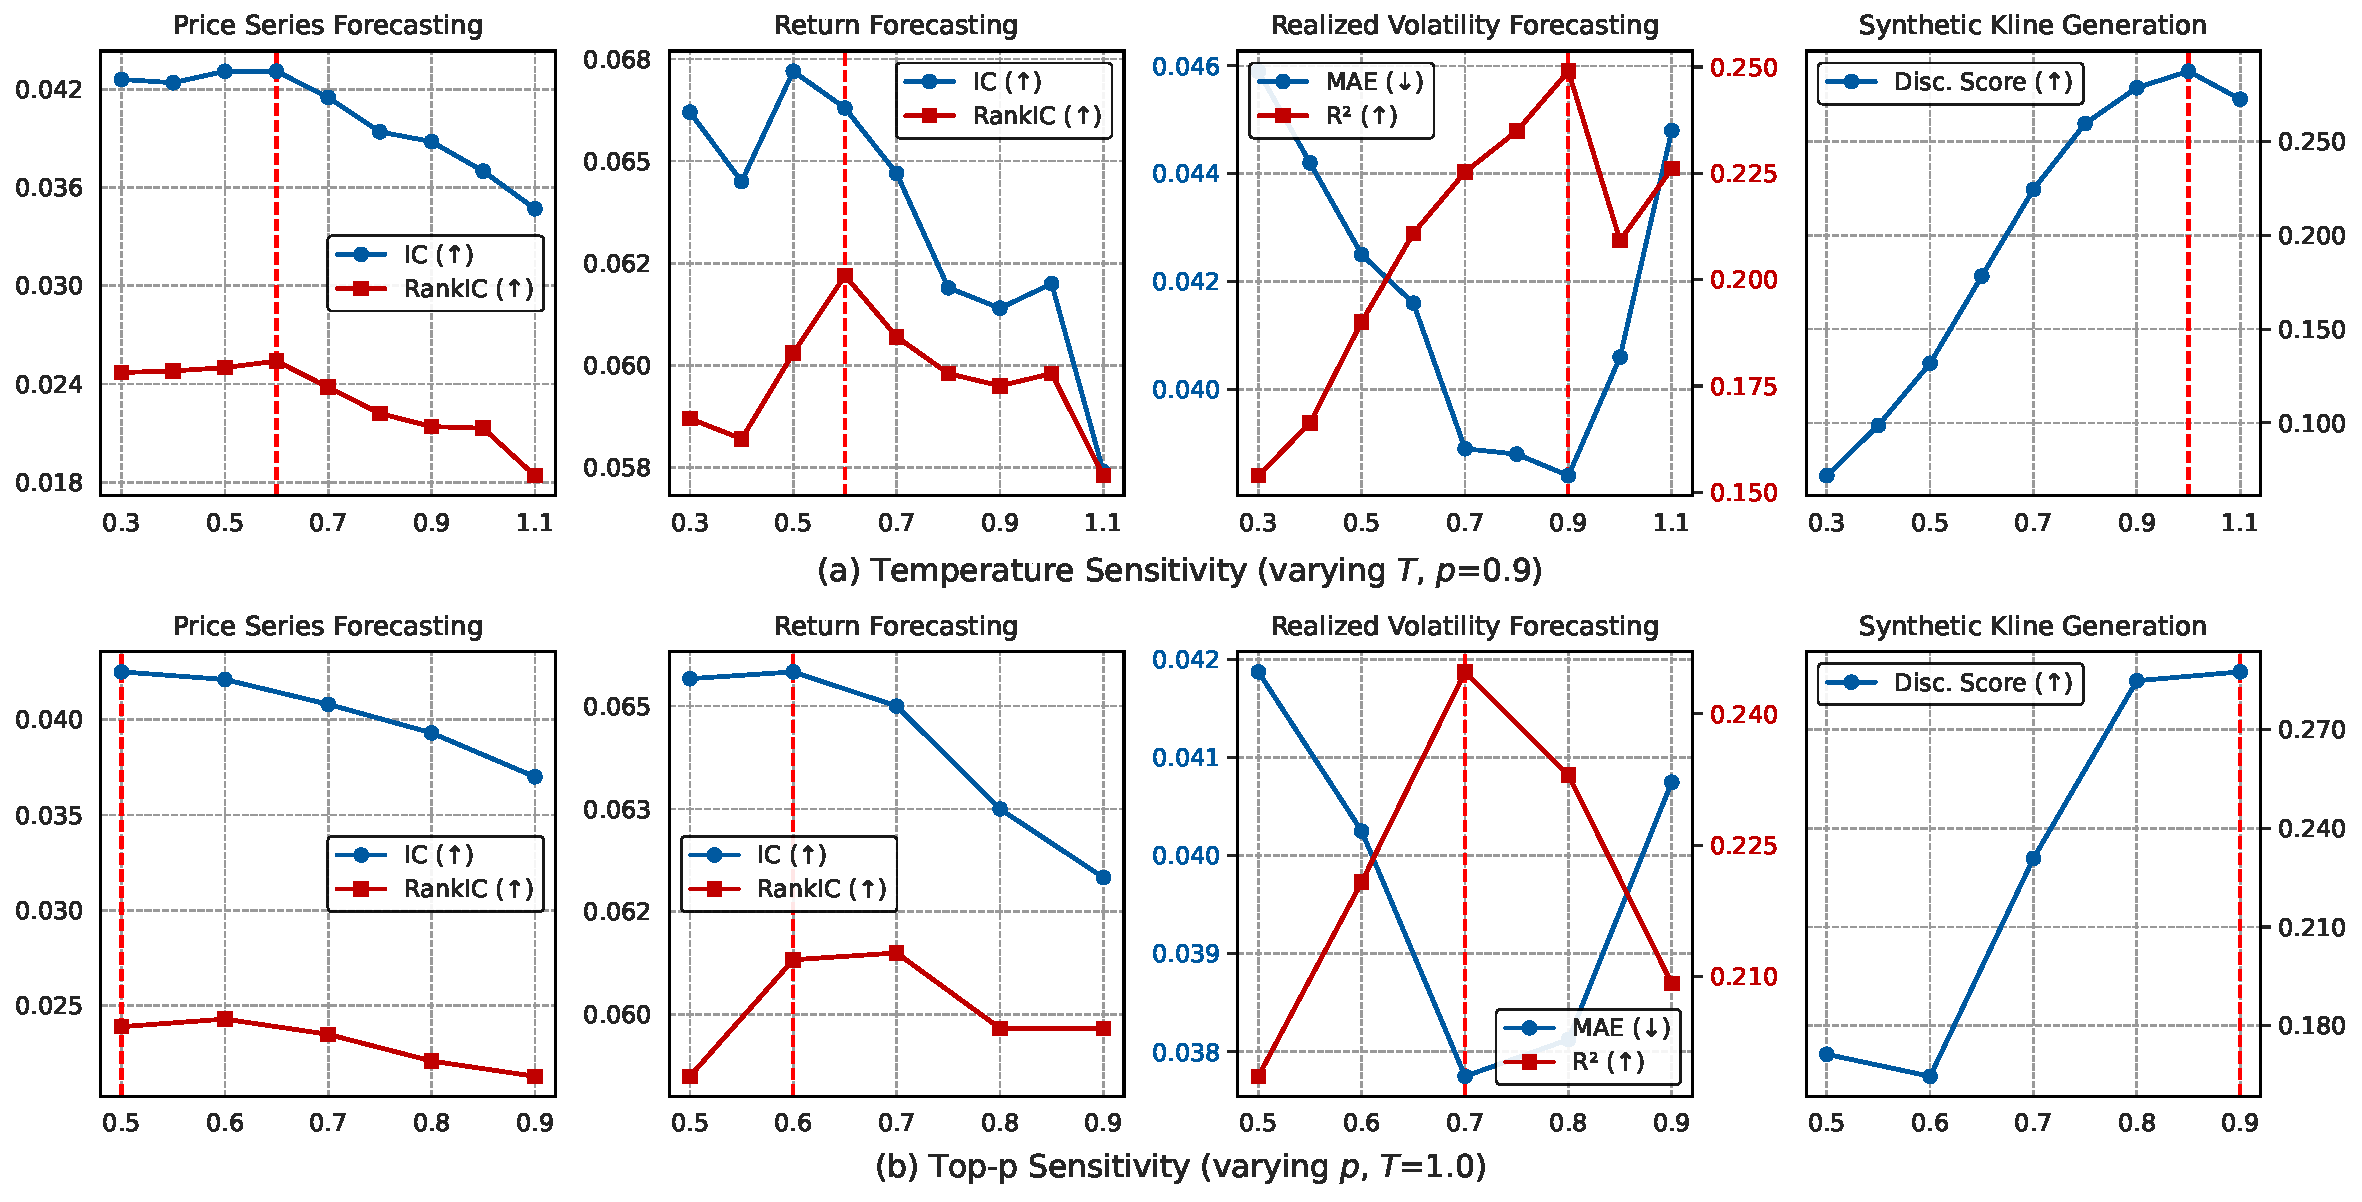
\includegraphics[width=1.0\textwidth]{img/sample_T_and_top_p_ablation.pdf}
    \caption{Sensitivity analysis of Kronos's performance on downstream tasks with respect to inference sampling hyperparameters. (a) Varying temperature $T$ while keeping top-$p=0.9$ fixed. (b) Varying top-$p$ while keeping temperature $T=1.0$ fixed. Optimal values, indicated by red dashed lines, are task-dependent, highlighting different requirements for precision versus diversity.}
    \label{fig:T_and_top_p}
\end{figure*}

\subparagraph{데이터셋과 생성 파라미터} We use data from two stock exchanges (in-distribution XSHG and out-of-distribution XTAI), as well as the cryptocurrency and forex datasets. We evaluate generation on two frequencies: 15-minute and daily. For the 15-minute frequency, we use a look-back window of 120 and generate a future sequence of length 96. For the daily frequency, the look-back is 96 and the generation horizon is 35. For each asset-frequency pair, we generate 6,000 synthetic sequences for evaluation.

\subparagraph{평가 지표}
\begin{itemize}
    \item \textbf{Discriminative Score:} To assess the fidelity of the generated data, we employ a post-hoc LSTM-based classifier to distinguish between real and synthetic sequences. The classifier consists of a single LSTM layer with a hidden dimension of 32. For training, we construct a balanced dataset of 6,000 samples (3,000 real, 3,000 synthetic) and a held-out test set of the same size and composition. The model is trained for 20 epochs with a batch size of 64, using the Adam optimizer (learning rate = 0.0005) and the binary cross-entropy (BCE) loss function. The Discriminative Score is defined as the classification error on the test set. A score approaching 0.5 indicates higher fidelity, signifying that the classifier struggles to differentiate generated data from real data.

    \item \textbf{Usefulness (TSTR):} To measure the practical usefulness of the synthetic data, we adopt the Train-on-Synthetic, Test-on-Real (TSTR) methodology. We train a post-hoc LSTM prediction model to forecast a future K-timestep window given a historical one. This model comprises two LSTM layers with a hidden dimension of 64. It is trained exclusively on 6,000 generated synthetic sequences for 20 epochs using the Adam optimizer (learning rate = 0.001) and a batch size of 64, with the Mean Squared Error (MSE) loss as the objective function. The look-back and horizon windows are set to (80, 16) for 15-minute data and (30, 5) for daily data, respectively. The trained model is then evaluated on the original, real test data. The final usefulness score is reported as the average Information Coefficient (IC) and Rank Information Coefficient (RankIC) of the predicted price series.
\end{itemize}

\paragraph{투자 시뮬레이션 설정}

To evaluate the practical profitability of Kronos and other baselines in real-world markets, we conduct an investment simulation on the Chinese A-share market. For simplicity, regarding the Zero-shot Time Series Models, we only select the largest-sized model from each family for comparison.

\subparagraph{데이터} Our empirical analysis utilizes daily market data for the Chinese A-share market, sourced from the Qlib platform~\cite{yang2020qlib}, an open-source framework for quantitative finance. To promote transparency and reproducibility, we apply no additional filtering or preprocessing to the data, using it in its original, unprocessed state. Furthermore, we conduct all backtesting simulations within the Qlib framework. This approach leverages its integrated backtesting engine to ensure a standardized and consistent evaluation protocol for all models under review.

\subparagraph{전략} We employ the top-$k$/drop-$n$ portfolio construction strategy. On each trading day, all stocks in the investment universe are ranked based on their predicted return signal. An equal-weight portfolio is formed by taking long positions in the top $k$ stocks. To manage turnover and trading costs, a maximum of $n$ stocks are bought or sold daily, and a minimum holding period of 5 days is enforced for all positions.

\subparagraph{신호와 백테스트}

The predictive signal is formulated as an expected return derived from a multi-step price forecast over a horizon of $H$ days. This signal generation pipeline is applied uniformly to all models under evaluation, including Kronos and the baselines, to ensure a fair comparison. For any given stock on trading day $t$, a sequence of forecasted closing prices for the subsequent $H$ days, denoted as $\{\hat{p}_{t+i}\}_{i=1}^{H}$, is first generated by the respective model. The signal, which we term the $H$-day average expected return ($R_{t \to t+H}$), is then calculated by comparing the arithmetic mean of these forecasted prices to the current closing price $p_t$:
\begin{equation}
R_{t \to t+H} = \frac{\left(\frac{1}{H}\sum_{i=1}^{H} \hat{p}_{t+i}\right) - p_t}{p_t}
\end{equation}
In our experiments, we set the forecast horizon to $H=10$. All price forecasts are generated using daily K-line data with a 90-day look-back window. This methodology is designed to produce a robust signal by averaging the forecasted price path, thereby mitigating the influence of short-term prediction noise and capturing the underlying trend more effectively.

Backtests are performed on the constituents of the CSI 300 and CSI 800 indices. These indices are chosen as they represent two key segments of the Chinese A-share market: the CSI 300 comprises large-cap, highly liquid stocks, while the CSI 800 provides broader market coverage by including both large- and mid-cap stocks. This allows for a comprehensive assessment of the model's performance across different market segments.


\subparagraph{파라미터와 비용} For the CSI 300 index, we set $k=50$ and $n=5$. For the broader CSI 800 index, we set $k=200$ and $n=10$. The relatively large portfolio sizes are chosen to ensure diversification and produce more stable backtesting results, reducing the influence of idiosyncratic stock movements. To ensure a realistic performance assessment, a conservative transaction cost of 0.15\% is applied to each trade.

\begin{figure*}[t!]
    \centering
    \begin{minipage}[t]{1.0\columnwidth}
        \centering
        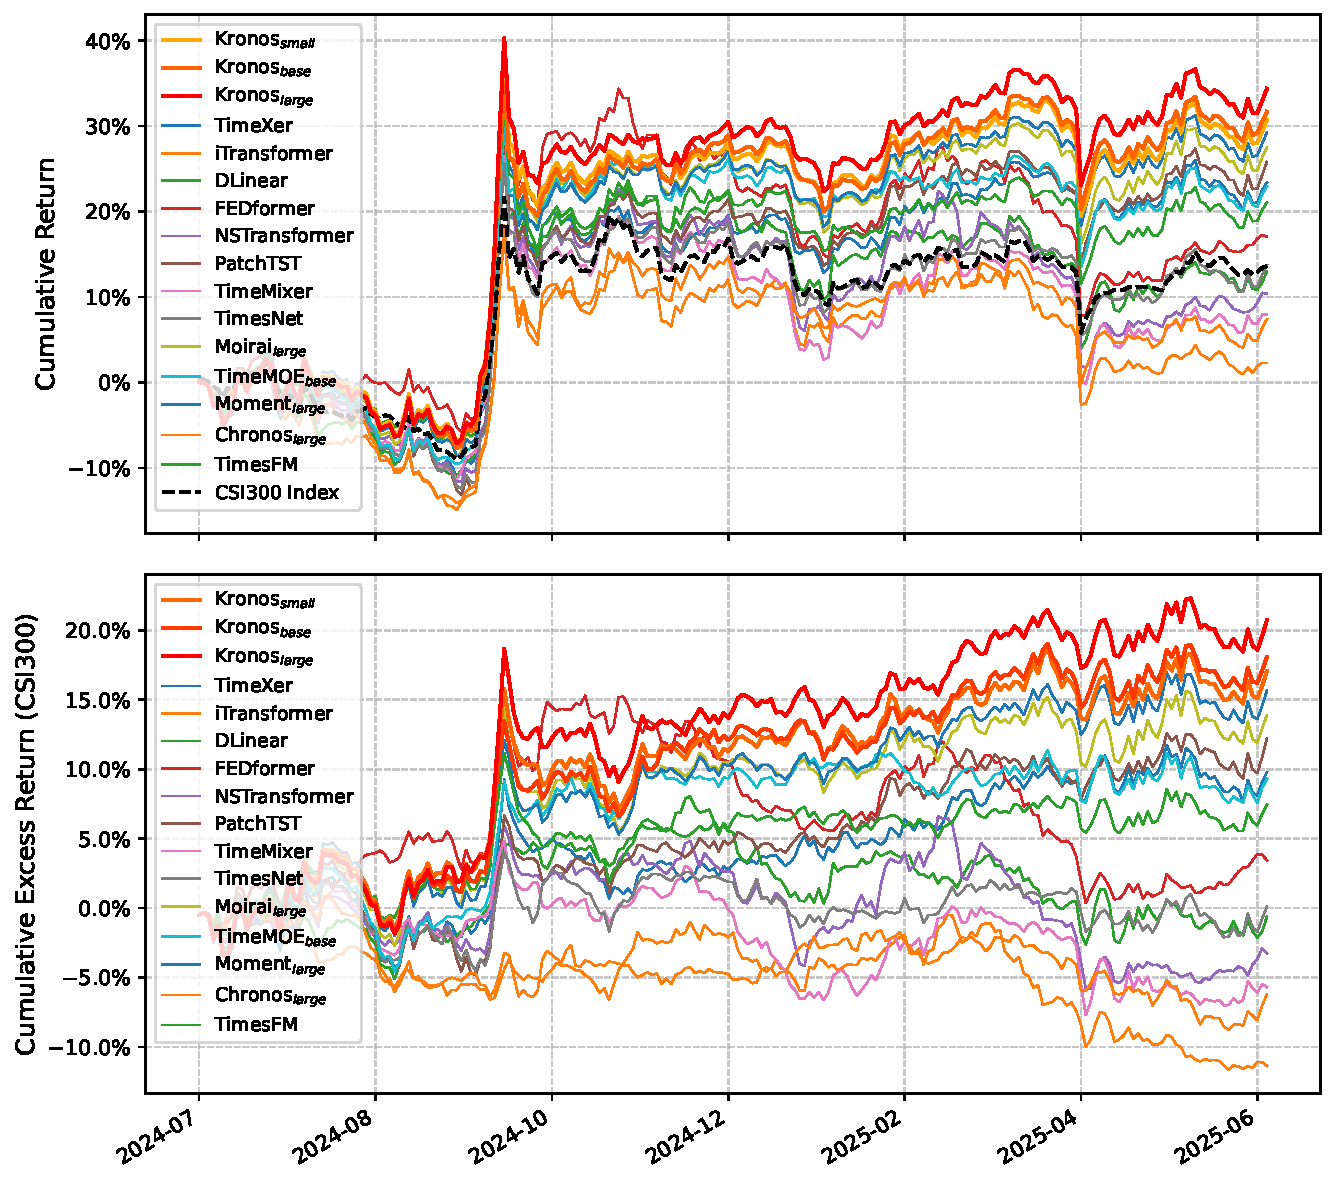
\includegraphics[width=\columnwidth]{img/backtest_csi300.pdf}
        \caption*{ (a) CSI300 Index}
    \end{minipage}
    \hspace{0.02\columnwidth}
    \begin{minipage}[t]{1.0\columnwidth}
        \centering
        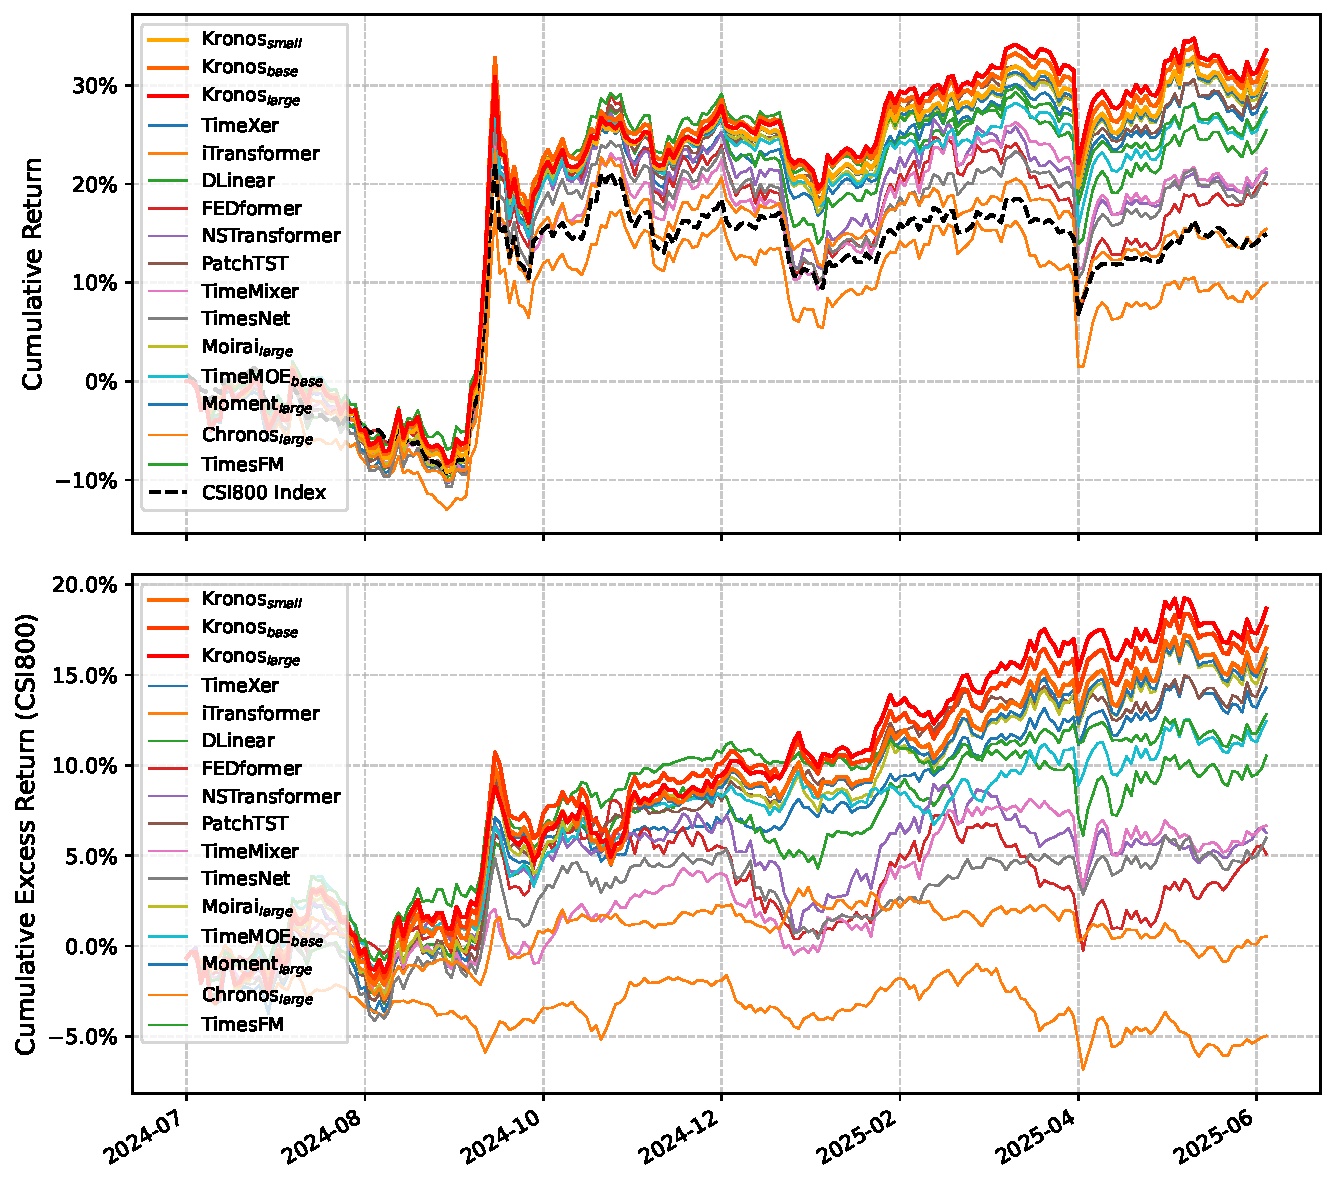
\includegraphics[width=\columnwidth]{img/backtest_csi800.pdf}
        \caption*{ (b) CSI800 Index}
    \end{minipage}
    \caption{서로 다른 모델이 생성한 신호를 사용한 백테스트의 누적 수익률 곡선.}
    \label{fig:backtest_profit}
\end{figure*}

\subsection{제거 연구 베이스라인 세부 사항}
\label{sec:ablation_baselines}

To investigate the architectural choices of Kronos, we design three baseline variants for our ablation study (Table~\ref{tab:ablation_study_refined}). Each variant targets a different modeling paradigm, allowing us to isolate the benefits of our proposed discrete, sequential framework. Below we provide a detailed description of each model.

\noindent\textbf{Direct-AR.} This model serves as a standard autoregressive forecasting baseline in the continuous space. Given a sequence of input features $\{x_1, \dots, x_T\}$, each feature vector $x_t \in \mathbb{R}^D$ is first mapped to a higher-dimensional embedding via a linear projection. The sequence of embeddings is then processed by a Transformer decoder backbone. The model is trained to directly predict the value of the next time step, $\hat{x}_{T+1}$, from the historical context. The training objective is to minimize the Mean Squared Error (MSE) between the predicted and ground-truth values. This approach represents the most common regression-based formulation for time series forecasting.

\noindent\textbf{Prob-AR.} This is a probabilistic forecasting model operating in the continuous space. Following established practices~\cite{yao2024towards}, instead of a point estimate, Prob-AR predicts the parameters of a probability distribution for the next time step. We use a mixture of four Student-t distributions to model the predicted distribution. The probability density function (PDF) for a random variable $x$ following a single Student-t distribution is:
\begin{equation}
p(x | \nu, \mu, \sigma) = \frac{\Gamma(\frac{\nu+1}{2})}{\Gamma(\frac{\nu}{2})\sqrt{\pi\nu}\sigma} \left(1 + \frac{1}{\nu}\left(\frac{x-\mu}{\sigma}\right)^2\right)^{-\frac{\nu+1}{2}}
\end{equation}
where $\nu > 0$, $\mu \in \mathbb{R}$, and $\sigma > 0$ are the degrees of freedom, location, and scale parameters, respectively, and $\Gamma(\cdot)$ is the gamma function. The model employs independent linear layers to predict the parameters for each of the four components—degrees of freedom ($\nu_k$), location ($\mu_k$), scale ($\sigma_k$), and mixture weights ($w_k$). To ensure parameter validity, a softplus transformation is applied to $\nu_k$ and $\sigma_k$ to enforce positivity, and a softmax function is applied to the weights $w_k$ to ensure they form a valid probability distribution. The model is trained by minimizing the Negative Log-Likelihood (NLL) of the true value under the predicted mixture distribution.

\noindent\textbf{Kronos-Parallel.} This variant is a direct ablation of the sequential subtoken generation mechanism within Kronos. While it shares the same input quantization and discrete prediction space as Kronos, it removes the intra-block module. After the Transformer backbone produces a context vector from the input history, a single prediction head is used to concurrently predict the logits for both subtokens of the next time step. The training objective is the sum of the cross-entropy losses for each subtoken, optimized jointly.

\subsection{실험 환경}
\label{sec:exp_environment}

All experiments are conducted within a Kubernetes (k8s) cluster. For all computational tasks, we utilize three identical pods. Each pod is provisioned with a dedicated set of resources comprising 96 CPU cores (Intel Xeon Gold 6330 @ 2.00 GHz), 200 GB of system memory (RAM), and eight NVIDIA GeForce RTX 4090D GPUs. This configuration provides a total of 24 GPUs, which are collectively employed for model training and all subsequent evaluations.

The software environment is containerized and standardized across all pods. The primary components and their versions are detailed below:
\begin{itemize}
    \item \textbf{Operating System:} Ubuntu 24.04.1 LTS
    \item \textbf{Software versions:} Python 3.13.2, PyTorch 2.7.0, NumPy 1.26.2, Pandas 2.2.2, Matplotlib 3.9.3, Hugging Face Hub (`huggingface\_hub') 1.57.4
\end{itemize}


\section{추가 결과}

\subsection{추론 샘플링 하이퍼파라미터의 영향}
\label{sec:sampling_hyperparams}

The autoregressive generation process of Kronos is governed by sampling strategies that introduce controlled stochasticity, namely temperature scaling ($T$) and top-$p$ (nucleus) sampling. The choice of these hyperparameters can significantly influence model performance on different downstream tasks. To provide guidance on their optimal settings, we conduct a sensitivity analysis. Figure~\ref{fig:T_and_top_p} illustrates the performance of Kronos across our four main tasks while varying one hyperparameter and holding the other constant.

As shown in Figure~\ref{fig:T_and_top_p}, the optimal sampling hyperparameters are task-dependent. For forecasting tasks (price series and return), which demand precision, lower temperatures (e.g., $T \approx 0.6$) are preferable. This sharpens the next-token distribution, compelling the model towards more deterministic and high-confidence predictions. Conversely, realized volatility forecasting and synthetic K-line generation benefit from greater stochasticity, achieving optimal performance at temperatures closer to 1.0. A higher temperature encourages the generation of more diverse sequences, which is essential for capturing the probabilistic nature of volatility and for producing realistic, non-repetitive market data.

The analysis of top-$p$ sampling reveals a similar pattern: forecasting tasks favor smaller $p$ values to restrict the sampling pool, whereas generative tasks perform better with a larger nucleus ($p \ge 0.9$) to preserve diversity. When comparing the two techniques, we observe that temperature scaling generally offers more effective and nuanced control, leading to slightly better peak performance across tasks. This suggests that the global probability rescaling of temperature may be a more suitable tuning mechanism than the hard truncation of nucleus sampling.

\subsection{토크나이저 아키텍처 제거 연구}
\label{sec:tokenizer_ablation}
We perform an ablation study on the tokenizer architecture to justify our design choices. We compare our proposed Transformer-based tokenizer using a hierarchical loss against two alternatives: (1) a Transformer-based tokenizer with a standard, non-hierarchical reconstruction loss and (2) a CNN-based architecture with a comparable parameter count. All models are trained with a vocabulary size of $2^{18}$.

\begin{table}[ht]
\centering

\resizebox{\columnwidth}{!}{%
\begin{tabular}{@{}l S[table-format=1.4] S[table-format=1.4]@{}}
\toprule
\textbf{토크나이저 아키텍처} & {\textbf{MAE} ($\downarrow$)} & {\textbf{MSE} ($\downarrow$)} \\
\midrule
\textbf{Transformer w/ Hierarchical Loss (Ours)} & 0.0785 & 0.0203 \\
Transformer w/ Standard Loss                   & 0.0781 & 0.0202 \\
\midrule
CNN-based                                      & 0.0916 & 0.0251 \\
\bottomrule
\end{tabular}%
}
\caption{
    Ablation study on the K-line tokenizer architecture. We compare our proposed Transformer-based tokenizer, which employs a hierarchical reconstruction loss, against two key variants: a Transformer-based tokenizer with a standard reconstruction loss and a CNN-based architecture. All models are trained with a vocabulary size of $2^{18}$. The table reports reconstruction quality measured by MAE and MSE.
}
\label{tab:tokenizer_ablation}
\end{table}

As shown in Table~\ref{tab:tokenizer_ablation}, the results indicate that Transformer-based architectures outperform the CNN-based model in reconstruction quality, highlighting the effectiveness of self-attention for capturing dependencies in K-line data. More importantly, our model with hierarchical loss achieves reconstruction quality nearly identical to that of the standard loss variant. This confirms that our approach successfully engineers a coarse-to-fine structure within the tokens—a property beneficial for the subsequent autoregressive model—without a notable trade-off in representational fidelity.

\subsection{K-line 재구성 시각화}

Figure~\ref{fig:recon_case} visualizes our tokenizer's reconstruction results on a diverse set of financial instruments. The plots show that the reconstructed `Close Price' and `Volume' series closely track the ground truth, confirming that our tokenizer effectively preserves the essential dynamics of the original continuous data within its discrete token representation.
% We note that due to the clipping of normalized input values to the range $[-5, 5]$ (see Appendix~\ref{sec:input_processing}), the tokenizer does not fully capture extreme outliers. This is a deliberate trade-off, as we find it enhances training stability and ultimately improves the generation quality of the subsequent autoregressive model.

\subsection{누적 수익률 곡선 시각화}

Figure~\ref{fig:backtest_profit} presents the cumulative return curves derived from backtesting using predictive signals by different models. As illustrated, Kronos consistently demonstrates superior performance, achieving the highest cumulative returns among the evaluated models.

\begin{table}[t]
  \centering
  \footnotesize
  \setlength{\tabcolsep}{4pt}

  \adjustbox{max width=\columnwidth}{
  \begin{tabular}{l *{6}{S}}
    \toprule
    \multirow{2}{*}{\textbf{Model}} & \multicolumn{2}{c}{\textbf{CSI300 Index}} & \multicolumn{2}{c}{\textbf{CSI800 Index}} & \multicolumn{2}{c}{\textbf{Average}} \\

    \cmidrule(lr){2-3} \cmidrule(lr){4-5} \cmidrule(lr){6-7}

    & \textbf{AER} & \textbf{IR} & \textbf{AER} & \textbf{IR} & \textbf{AER} & \textbf{IR} \\
    \midrule

    TimeXer       & 0.1035 & 0.7988 & 0.1509 & 1.5471 & 0.1272 & 1.1730 \\
    TimeMixer       & -0.0600 & -0.5721 & 0.0705 & 0.8113 & 0.0053 & 0.1196 \\
    iTransformer       & -0.1202 & -1.4441 & -0.0525 & -0.8558 & -0.0864 & -1.1500 \\
    PatchTST       & 0.1289 & 0.9895 & 0.1620 & 1.5033 & 0.1455 & 1.2464 \\
    TimesNet       & 0.1441 & 0.6558 & 0.0634 & 0.7225 & 0.1038 & 0.6892 \\
    DLinear       & -0.0066 & -0.0605 & 0.1112 & 1.2003 & 0.0523 & 0.5699 \\
    FEDformer       & 0.0362 & 0.2943 & 0.0539 & 0.5602 & 0.0451 & 0.4273 \\
    NSTransformer       & -0.0343 & -0.2889 & 0.0664 & 0.6979 & 0.0161 & 0.2045 \\

    \midrule

    $\text{Time-MOE}_{base}$       & 0.0985 & 0.8230 & 0.1315 & 1.3726 & 0.1150 & 1.0978 \\
    $\text{Moirai}_{large}$       & 0.1470 & 0.9747 & 0.1683 & 1.5215 & 0.1577 & 1.2481 \\
    TimesFM       & 0.0788 & 0.7357 & 0.1355 & 1.6427 & 0.1072 & 1.1892 \\
    $\text{Moment}_{large}$       & 0.1655 & 1.1993 & 0.1707 & 1.5361 & 0.1681 & 1.3677 \\
    $\text{Chronos}_{large}$       & -0.0659 & -0.7670 & 0.0056 & 0.0902 & -0.0302 & -0.3384 \\

    \midrule
    \textbf{$\text{Kronos}_{small}$} & 0.1805 & 1.2394 & 0.1772 & 1.6050 & 0.1789 & 1.4222 \\
    \textbf{$\text{Kronos}_{base}$} & \second{0.1911} & \second{1.3782} & \second{0.1867} & \second{1.6652} & \second{0.1889} & \second{1.5217} \\
    \textbf{$\text{Kronos}_{large}$} & \best{0.2193} & \best{1.4177} & \best{0.1974} & \best{1.8805} & \best{0.2084} & \best{1.6491}\\
    \bottomrule
  \end{tabular}}
  \caption{Full results of investment simulation. We report Annualized Excess Return (AER) and Information Ratio (IR). Best and second best results are marked with \best{red underline} and \second{blue underline}, respectively.
  }
  \label{tab:full_backtest_result}
\end{table}

\section{전체 실험 결과}
\label{sec:full_exp_results}

In this section, we present the complete experimental results for three forecasting tasks and the synthetic K-line generation task. For the forecasting tasks, we report the results for each asset, averaged over all tested frequencies.
Tables~\ref{tab:full_price_forecasting_1} and~\ref{tab:full_price_forecasting_2} show the results of the price series forecasting experiments.
The outcomes for return forecasting are presented in Tables~\ref{tab:full_return_forecasting_1} and~\ref{tab:full_return_forecasting_2}, while those for realized volatility forecasting are in Tables~\ref{tab:full_volatility_forecasting_1} and~\ref{tab:full_volatility_forecasting_2}.
Furthermore, for the synthetic K-line generation task, Figures~\ref{fig:gen_visual_1} and~\ref{fig:gen_visual_2} provide visualizations of the \textit{diversity} of the generated sequences by different models. The results for the discriminative score and predictive usefulness are presented in Table~\ref{tab:generate_discriminative} and Table~\ref{tab:generate_usefulness}, respectively. Finally, the results of the investment simulation experiment are presented in Table~\ref{tab:full_backtest_result}.

\section{예측 사례}

Figures~\ref{fig:pred_case_1} to \ref{fig:pred_case_5} present the forecasting results of our proposed model, Kronos, against several baselines.
We select a few representative assets and showcase the predictions for two key features: closing price and trading volume.
As observed, the forecasts from Kronos not only achieve competitive predictive performance but also exhibit a strong qualitative resemblance to the ground-truth series.
Notably, our model adeptly captures the characteristic dynamics and patterns of the actual price and volume sequences, producing forecasts that are not only accurate but also visually plausible.

\section{논의}
\label{sec:discussion}


\subsection{K-line 데이터는 단기 자본시장 가격 움직임을 이끌 충분한 정보를 내포하는가? (Q1)}

% In capital markets, the factors driving price movements can be broadly categorized into two types: short-term factors, which are highly volatile and have immediate effects, and long-term factors, which exhibit clear trends and have a profound impact on value formation.

% Long-term factors determine the overall direction and valuation level of the market, while short-term factors generate volatility and trading opportunities.

% A large number of empirical research shows that price and trading volume together can reflect the information embedded in short-term drivers such as macroeconomic announcements, corporate events, and market sentiment.

In capital markets, the determinants of price dynamics are conventionally bifurcated into:

\begin{itemize}
\item \textbf{Long‐term driving factors}, which manifest as persistent trends and exert a lasting influence on intrinsic value;
\item \textbf{Short‐term driving factors}, which are typified by elevated volatility and immediate market impact.

\end{itemize}

Long‐term driving factors establish the market’s prevailing trajectory and valuation benchmarks, whereas short‐term ones introduce transient volatility and generate discrete trading opportunities.

Extensive empirical evidence demonstrates that kline data (\textbf{OHLCVA}, including \textbf{price} and \textbf{trading volume})~\cite{kim1991trading}, when analyzed in tandem, effectively encapsulate the informational content of short‐term driving factors—such as macroeconomic data releases ~\cite{flannery2002macroeconomic}, corporate event disclosures~\cite{kim1991trading}, and shifts in investor sentiment~\cite{baker2006investor, da2011search}.



The detail discussion about the above empirical evidences is beyond the scope of this paper.


% \subsection{Kronos의 토크나이저가 작동하는 이유는 무엇인가? (Q2)}

% The motivation for using vision‑inspired quantization (BSQ) in time-series modeling could be discussed from the perspectives of artificial intelligence model and financial market micro-structure.

% \subsubsection{Noise suppression and stability}

% % High‑frequency K‑line bars (e.g., 5‑minute or 15‑minute intervals) often contain a lot of  noises (like quote flickers and small outlier trades). BSQ reduces these noises by first mapping each continuous feature vector onto a fixed set of points on a sphere and then converting it to a binary token. The outcome is a steadier ``token sequence'' that filters out those fleeting blips and instead highlights genuine shifts in the market’s structure (for example, market trends, regime changes or sudden liquidity sweeps).

% Using quantization to transform regression into classification-style problems could improve the stability and reliability of financial forecasting models.

% Additionally, by projecting embeddings onto the unit sphere before binarizing, BSQ~\cite{zhao2024image} guarantees
%     \[
%       \mathbb{E}_u \,\big\|u - \widehat u\big\|\;<\;\sqrt{2 - 2/\sqrt{L}}\;<\sqrt{2},
%     \]
% so the distortion is strictly upper‑bounded and shrinks as the codebook dimension \(L\) grows.
% In contrast, the sign-based quantization without normalization (LFQ) has unbounded error.


% In financial markets, there are outliers—for example, a “flash‑crash” data point caused by an anomalous trade match in liquidity shortage. The bounded quantization error prevents extreme outlier values from producing arbitrarily large approximation errors.


% \subsubsection{Compact, discrete state space}
% Discretizing into a small set of binary codes transforms high‑dimensional price‐volume vectors into a compact token sequence. This drastically reduces the vocabulary size for downstream sequence models, improving sample efficiency and reducing overfitting—especially critical when modeling rare quotes under various shocks.


% \begin{table}[th]
% \centering
% \sisetup{table-format=1.4}
% \begin{tabular*}{\columnwidth}{@{\extracolsep{\fill}} l S S}
% \toprule
% \textbf{Dataset} & {\textbf{MAE}} & {\textbf{MSE}} \\
% \midrule
% XHKG     & 0.0798 & 0.0201 \\
% XIDX     & 0.0903 & 0.0265 \\
% XJPX     & 0.0776 & 0.0207 \\
% XKLS     & 0.0871 & 0.0220 \\
% XKRX     & 0.0849 & 0.0236 \\
% XNAS     & 0.0836 & 0.0223 \\
% XNSE     & 0.0805 & 0.0208 \\
% XSHG     & 0.0755 & 0.0148 \\
% XTAI     & 0.0785 & 0.0195 \\
% Crypto   & 0.0417 & 0.0044 \\
% Forex    & 0.0541 & 0.0081 \\
% \midrule
% \textbf{Average} & \bfseries 0.0770 & \bfseries 0.0192 \\
% \bottomrule
% \end{tabular*}
% \caption{
% Reconstruction performance of different datasets.(The full names of \textit{Dataset} colume can be found in Appendix~\ref{sec:exp_setup_details} section \textit{Forecasting Task Setup}.)
% }
% \label{tab:reconstruction_performance}
% \end{table}


% As is shown in Table \ref{tab:codebook_usage}, the code usage of BSQ reaches 97.66\% at the coarse level and 85.25\% at the fine level in Krono's tokenizer, which contributes to a more nuanced representation of market microstructure.


\subsection{Kronos의 토크나이저가 작동하는 이유는 무엇인가? (Q2)}

The effectiveness of our vision-inspired quantization (BSQ) tokenizer can be analyzed from two key perspectives: its inherent noise suppression and its ability to create a structured, discrete state space suitable for sequence modeling.

\subsubsection{노이즈 억제와 안정성}
Financial time-series data is often corrupted by noise and subject to extreme outliers, such as ``flash-crash'' events caused by anomalous trades. A primary challenge for regression-based models is that such outliers can lead to unbounded approximation errors, severely degrading model stability~\cite{brownlees2006financial}.

Our approach addresses this by transforming the representation learning into a more robust, classification-like framework. By quantizing continuous price-volume embeddings, we effectively cap the influence of any single data point. Specifically, BSQ's projection of embeddings onto a unit sphere prior to binarization guarantees that the expected distortion is strictly upper-bounded~\cite{zhao2024image}:
\[
  \mathbb{E}_u \,\big\|u - \widehat u\big\|\;<\;\sqrt{2 - 2/\sqrt{L}}\;<\sqrt{2}.
\]
This bound tightens as the codebook dimension \(L\) increases. In contrast, simpler methods like sign-based quantization without normalization (e.g., LFQ) lack such a guarantee, leaving them vulnerable to arbitrarily large errors from outlier inputs~\cite{zhao2024image}. This bounded error property is crucial for building reliable financial forecasting models.

\subsubsection{작고 이산적인 상태 공간에서의 학습}
High-frequency financial data exists in a high-dimensional, continuous state space, posing significant challenges for sequence models. Our tokenizer maps these infinite states into a finite, discrete vocabulary of tokens. This discretization serves as a powerful form of regularization with two main benefits~\cite{rabanser2020effectiveness}:

\begin{itemize}
    \item \textbf{Improved Sample Efficiency and Generalization}: Instead of learning a complex function over a continuous space, a downstream model like a Transformer learns to predict transitions and patterns among a finite set of abstract states (tokens). This simplifies the learning task. Different but semantically similar input vectors can be mapped to the same token, effectively increasing the number of observations for each discrete state. This allows the model to learn robust patterns from fewer examples, which is particularly critical for modeling rare market phenomena like responses to liquidity shocks, where data is sparse.
    \item \textbf{Reduced Overfitting}: The quantization process inherently discards fine-grained, potentially noisy variations within each quantization cell. This prevents the model from fitting to spurious artifacts in the training data.
\end{itemize}

\begin{table}[h!]
\centering

\resizebox{\columnwidth}{!}{%
\begin{tabular*}{\columnwidth}{@{\extracolsep{\fill}} ccc}
\toprule
\textbf{코드북 유형} & \textbf{크기} & \textbf{사용률} \\
\midrule
Coarse-Level-Subtoken Codebook      & $2^{10}$ & 97.66\% \\
Fine-Level-Subtoken Codebook        & $2^{10}$ & 85.25\% \\
\bottomrule
\end{tabular*}}

\caption{거친 수준 서브토큰과 세밀한 수준 서브토큰의 코드북 사용률.}
\label{tab:codebook_usage}
\end{table}

\begin{table*}[t!]
\centering

\resizebox{\textwidth}{!}{%
\begin{tabular}{@{}l c c r r r r c@{}}
\toprule
\textbf{설정} & \textbf{Splits ($n$)} & \textbf{Sub-Vocab ($2^{k/n}$)} & \textbf{코어 파라미터 (M)} & \textbf{어휘 파라미터 (M)} & \textbf{융합 파라미터 (M)} & \textbf{총 파라미터 (M)} & \textbf{토큰당 추론 단계} \\
\midrule
No Split & 1 & 1,048,576 & 97.5 & 1744.8 & 0.0 & 1842.3 & 1$\times$ \\
\textbf{Ours} & \textbf{2} & \textbf{1,024} & \textbf{97.5} & \textbf{3.4} & \textbf{1.4} & \textbf{102.3} & \textbf{2$\times$} \\
More Splits & 4 & 32 & 97.5 & 0.2 & 2.8 & 100.5 & 4$\times$ \\
& 5 & 16 & 97.5 & 0.1 & 3.5 & 101.1 & 5$\times$ \\
\bottomrule
\end{tabular}%
}
\caption{
    Trade-off analysis for factorizing a $k=20$ bit token into $n$ subtokens, based on the $\text{Kronos}_{base}$ architecture. The model's core Transformer blocks have $\approx$97.5M parameters.
}
\label{tab:factorization_analysis_revised}
\end{table*}

The effectiveness of our tokenizer is further evidenced by its codebook utilization. As shown in Table \ref{tab:codebook_usage}, the code usage of BSQ reaches 97.66\% at the coarse level and 85.25\% at the fine level. Such high utilization indicates that our method creates an expressive vocabulary, effectively partitioning the feature space without suffering from codebook collapse (where many codes are left unused)~\cite{zhu2024addressing}. This expressiveness provides the rich foundation necessary for a model to capture the nuanced and diverse states of market microstructure.

% Table \ref{tab:reconstruction_performance} summarizes the reconstruction performance across different markets and asset classes, while Figure \ref{fig:recon_case} presents visualization examples of K-line reconstruction cases.

Additionally, the vocabulary is stratified into three categories based on usage frequency: (a) high-frequency, (b) low-frequency, and (c) unused tokens. To investigate their representational characteristics, we conduct an analysis where we replace the final token of an encoded sequence with a token from each category and then decode it back to a K-line. Figure \ref{fig:token_show_case} presents the results of this procedure. We observe a clear correspondence between token frequency and pattern typicality. High-frequency tokens (a) map to common K-bar shapes, indicative of stable market conditions. Conversely, low-frequency (b) and unused (c) tokens generate more extreme and atypical K-bars, such as those with long bodies or wicks, signifying rare, high-volatility events. This suggests that the learned codebook captures a meaningful semantic hierarchy, effectively distinguishing between common and significant market patterns based on token frequency.



\subsubsection{꼬리 민감성을 위한 초구면 기하}
In financial contexts, market returns and price changes often exhibit heavy tails (or fat tails)~\cite{mandelbrot1963variation}. The heavy-tail distribution of price changes is one of the key sources of trading profits in quantitative investment and cannot be ignored.

Unlike standard vector-quantization on the Euclidean sphere, BSQ’s binary encoding preserves angular information very efficiently, making it more sensitive to fat-tail data that manifest as sharp directional changes in feature space. This aligns well with how microstructure events often appear as abrupt shifts in the “direction” of the joint price-volume vector~\cite{podobnik2009cross}.

Figure~\ref{fig:kline_reconstruction_tradewar} illustrates the tokenizer's ability to capture and reconstruct the long-tailed market microstructure under short-term high volatility and during extreme gap events (in the economic context of Trump’s Trade War~\cite{mckibbin2025global}).

Above all, we summarize the concrete advantages of BSQ for K-line time series data, leveraging its ability to preserve angular information and capture sharp directional changes, which are crucial for modeling financial time series with heavy tails and abrupt shifts due to microstructure events.

\subsection{서브토큰 분해 분석 (Q3)}
\label{sec:subtoken_factorization}

Our methodology factorizes a $k$-bit token into $n$ subtokens to manage a large vocabulary size. A key design choice is the number of factors, $n$. While further factorization (e.g., $n>2$) could reduce sub-vocabulary sizes even more (e.g., from $2^{10}$ to $2^5$ for a $k=20$ token), we argue that $n=2$ offers the best trade-off between parameter efficiency and inference latency.

This factorization introduces a fundamental trade-off. On one hand, it significantly reduces the size of \textbf{vocabulary-dependent parameters} in the input embedding and output projection layers, replacing a single large table for a $2^k$ vocabulary with $n$ smaller tables for $2^{k/n}$ sub-vocabularies. On the other hand, it introduces two costs: (1) a new \textbf{fusion layer} ($W_{\text{fuse}}$ in Equation~\ref{eq:embedding}), whose parameters $(n \times \mathbf{d}_{\text{model}}) \times \mathbf{d}_{\text{model}}$ grow linearly with $n$, and (2) increased \textbf{inference latency}, as generating a full token requires $n$ sequential autoregressive steps.

Table~\ref{tab:factorization_analysis_revised} quantifies this trade-off for our $\text{Kronos}_{base}$ model. The most significant parameter reduction is achieved by moving from no factorization ($n=1$) to a 2-way split. This single step reduces vocabulary-dependent parameters by over 99.8\% (from $\approx$1.7B to 3.4M), shrinking the total model size by nearly 95\% and making a large effective vocabulary computationally feasible.

However, further factorization yields diminishing returns while incurring rising costs. Moving from $n=2$ to $n=4$ reduces vocabulary parameters by only 3.2M, a saving that is partially offset by a 1.4M increase in fusion layer parameters. This results in a marginal total parameter reduction of just $\approx$2\%. As $n$ increases to 5, the overhead from the fusion layer outweighs the savings from the smaller vocabularies, causing the total parameter count to increase. Crucially, these marginal or negative parameter benefits come at a direct and substantial latency cost: moving from $n=2$ to $n=4$ doubles the number of sequential generation steps required per token.

In summary, our choice of $n=2$ represents an effective balance. It captures the vast majority of the parameter-reduction benefits, making our large vocabulary practical, while avoiding the significant latency penalties and growing architectural overhead associated with finer-grained splits.


\onecolumn

\begin{footnotesize}
\begin{center}
\begin{longtable}{@{\extracolsep{\fill}} l l l r r l @{}}

    \toprule
    \textbf{거래소 / 국가} & \textbf{자산 유형} & \textbf{시간 주기} & \textbf{\# Assets} & \textbf{\# Observations} & \textbf{시작일} \\
    \midrule
    \endfirsthead
    \multicolumn{6}{c}%
    {{\bfseries\tablename\ \thetable{} -- Continued from previous page}} \\
    \toprule
    \textbf{거래소 / 국가} & \textbf{자산 유형} & \textbf{시간 주기} & \textbf{\# Assets} & \textbf{\# Observations} & \textbf{시작일} \\
    \midrule
    \endhead
    \midrule
    \multicolumn{6}{r@{}}{\textit{다음 페이지에 계속}} \\
    \endfoot

    \bottomrule \\
    \caption{다중 거래소, 다중 자산 K-line 데이터셋의 기술 통계. 시간 프레임 약어는 다음과 같다: T (1분), H (1시간), D (1일), W (1주).}
    \label{tab:dataset_overview} \\
    \endlastfoot

    Binance            & 암호화폐,무기한 스왑             & T, 5T, 15T, 30T, H, D, W        & 997   & 1,237,002,843   & 2021/1/31 \\
        Athens Stock Exchange          & 주식, ETF             & D, W        & 180   & 226,315   & 2023/4/11 \\
        Beijing Stock Exchange         & 주식       & 5T, 15T, 30T, H, D, W & 272      & 10,197,628   & 2021/11/19 \\
        Brazil Stock Exchange          & 주식, ETF       & D, W & 2,058      & 1,315,290   & 2020/1/31 \\
        Moscow Exchange             & 주식, ETF       & D, W              & 514     &  567,351    & 2020/1/31 \\
        Euronext Amsterdam             & 주식, ETF           & D, W                  & 514    & 602,083    & 2020/1/31 \\
        Australian Securities Exchange     & 주식, ETF           & 5T, 15T, 30T, H, D, W              & 3,381    & 86,613,897    & 2020/1/31 \\
        Stock Exchange of Thailand            & 주식, ETF        & 5T, 15T, 30T, H, D, W                  & 1,664   & 49,590,394    & 2020/1/31 \\
        Bombay Stock Exchange & 주식, ETF       & 5T, 15T, 30T, H, D, W              & 5,491 & 284,428,211 & 2020/1/31 \\
        Euronext Brussels & 주식, ETF       & D, W              & 166 & 195,491 & 2020/1/31 \\
        Bucharest Stock Exchange & 주식, ETF       & D, W  & 247 & 176,080 & 2020/1/31 \\
        Budapest Stock Exchange & 주식, ETF       & D, W  & 50 & 57,586 & 2022/1/14 \\
        Buenos Aires Stock Exchange & 주식 & D, W  & 183 & 225,352 & 2020/1/31 \\
        Colombo Stock Exchange & 주식 & D, W  & 292 & 372,627 &  2020/1/31 \\
        Copenhagen Stock Exchange & 주식 & D, W  & 825 & 617,464 & 2020/1/31 \\
        Frankfurt Stock Exchange & 주식, ETF & D, W  & 17,054 & 21,547,744 & 2020/1/31 \\
        Ghana Stock Exchange &  주식 & D, W  & 44 & 57,690 & 2020/1/31 \\
        Hong Kong Stock Exchange & 주식, ETF & 5T, 15T, 30T, H, D, W & 3,500 & 359,434,220  & 2020/1/31 \\
        Japan Exchange Group &  주식, ETF & 5T, 15T, 30T, H, D, W & 4,467 & 280,601,980 &  2020/1/31 \\
        Indonesia Stock Exchange & 주식 & 5T, 15T, 30T, H, D, W & 935 & 38,627,125 &  2020/1/31 \\
        Borsa Istanbul &  주식 & D, W  & 627 & 784,147 &  2020/1/31 \\
        Johannesburg Stock Exchange & 주식, ETF & D, W  & 562 & 681,587 & 2020/1/31 \\
        Pakistan Stock Exchange & 주식, ETF & D, W  & 660 & 595,505 & 2020/1/31 \\
        Kuala Lumpur Stock Exchange & 주식, ETF & 5T, 15T, 30T, H, D, W & 1,150 & 45,938,559 & 2020/1/31 \\
        Korea Exchange & 주식, ETF & 5T, 15T, 30T, H, D, W & 2,928 & 205,061,301 & 2020/1/31 \\
        Lima Stock Exchange & 주식, ETF & D, W  & 166 & 63,503 & 2020/1/31 \\
        Euronext Lisbon & 주식, ETF & D, W  & 60 & 65,753 & 2020/1/31 \\
        London Stock Exchange & 주식, ETF & 5T, 15T, 30T, H, D, W & 8,660 & 177,947,624 & 2020/1/31 \\
        Luxembourg Stock Exchange & 주식 & D, W  & 5 & 7,598 & 2020/1/31 \\
        Madrid Stock Exchange & 주식, ETF & D, W  & 309 & 331,745 & 2020/1/31 \\
        Mexican Stock Exchange & 주식, ETF & D, W  & 775 & 937,637 & 2020/1/31 \\
        Nasdaq Stock Exchange & 주식, ETF & T, 5T, 15T, 30T, H, D, W & 8,725 & 2,478,662,459 & 2000/1/1 \\
        National Stock Exchange of India & 주식, ETF & 5T, 15T, 30T, H, D, W & 2,554 & 242,429,169 & 2020/1/31 \\
        New York Stock Exchange & 주식, ETF & T, 5T, 15T, 30T, H, D, W & 7,073 & 2,133,143,549 & 2000/1/1 \\
        Euronext Paris & 주식, ETF & D, W  & 1,781 & 1,981,059 & 2020/1/31 \\
        Philippine Stock Exchange & 주식, ETF & 5T, 15T, 30T, H, D, W & 351 & 4,388,378 & 2020/1/31 \\
        Prague Stock Exchange & 주식 & D, W  & 50 & 62,666 & 2020/1/31 \\
        Santiago Stock Exchange & 주식 & D, W  & 225 & 160,638 & 2020/1/31 \\
        Shenzhen Stock Exchange & 주식, ETF & T, 5T, 15T, 30T, H, D, W & 3,519 & 1,754,519,331 & 1990/12/19 \\
        Shenzhen Stock Exchange (B-shares) & 주식 & 5T, 15T, 30T, H, D, W & 46 & 4,198,702 & 2020/2/3 \\
        Shanghai Stock Exchange & 주식, ETF & T, 5T, 15T, 30T, H, D, W & 3,064 & 1,967,996,343 & 1990/12/19 \\
        Shanghai Stock Exchange (B-shares) & 주식 & 5T, 15T, 30T, H, D, W & 50 & 4,526,152 & 2020/2/3 \\
        Stockholm Stock Exchange & 주식, ETF & D, W  & 1,305 & 1,463,722 & 2020/1/31 \\
        SIX Swiss Exchange & 주식, ETF & D, W  & 1,981 & 2,451,675 & 2020/1/31 \\
        Taiwan Stock Exchange & 주식, ETF & 5T, 15T, 30T, H, D, W & 1,252 & 71,619,260 & 2020/1/31 \\
        Toronto Stock Exchange & 주식, ETF & D, W  & 3,035 & 3,356,561 & 2020/1/31 \\
        Vienna Stock Exchange & 주식 & D, W  & 98 & 123,643 & 2020/1/31 \\
        중국 & 선물 & T, 5T, 15T, D & 75 & 63,318,960 & 2010/1/1 \\
        \textbackslash & 외환 & 5T, 15T, 30T, H, D, W & 1,023 & 462,434,562 & 2020/1/31 \\
        호주 & 주가지수 & 5T, 15T, 30T, H, D, W & 40 & 183,158 & 2020/1/31 \\
        벨기에 & 주가지수 & D, W  & 5 & 8,109 & 2020/1/31 \\
        브라질 & 주가지수 & D, W  & 3 & 4,766 & 2020/1/31 \\
        캐나다 & 주가지수 & D, W  & 18 & 27,622 & 2020/1/31 \\
        중국 & 주가지수 & 5T, 15T, 30T, H, D, W & 597 & 55,884,065 & 2020/2/3 \\
        독일 & 주가지수 & D, W  & 18 & 28,622 & 2020/1/31 \\
        스페인 & 주가지수 & D, W  & 2 & 3,257 & 2020/1/31 \\
        프랑스 & 주가지수 & D, W  & 38 & 55,945 & 2020/1/31 \\
        영국 & 주가지수 & 5T, 15T, 30T, H, D, W   & 51 & 5,355,869  & 2020/1/31 \\
        그리스 & 주가지수 & D, W  & 1 & 1,589 & 2020/1/31 \\
        홍콩, 중국 & 주가지수 & 5T, 15T, 30T, H, D, W   & 4 & 453,016 & 2020/1/31 \\
        헝가리 & 주가지수 & D, W  & 1 & 1,602 & 2020/1/31 \\
        인도네시아 & 주가지수 & 5T, 15T, 30T, H, D, W  & 2 & 47,816 & 2020/1/31 \\
        인도 & 주가지수 & 5T, 15T, 30T, H, D, W  & 113 & 3,189,450 & 2020/1/31 \\
        일본 & 주가지수 & 5T, 15T, 30T, H, D, W  & 9 & 125,024 & 2020/1/31 \\
        한국 & 주가지수 & 5T, 15T, 30T, H, D, W  & 5 & 274,292 & 2020/1/31 \\
        멕시코 & 주가지수 & D, W  & 1 & 1,619 & 2020/1/31 \\
        말레이시아 & 주가지수 & D, W  & 2 & 3,145 & 2020/1/31 \\
        네덜란드 & 주가지수 & D, W  & 4 & 6,475 & 2020/1/31 \\
        파키스탄 & 주가지수 & D, W  & 3 & 3,184  & 2020/1/31 \\
        필리핀 & 주가지수 & D, W  & 2 & 3,187  & 2020/1/31 \\
        포르투갈 & 주가지수 & D, W  & 1 & 1,632 & 2020/1/31 \\
        루마니아 & 주가지수 & D, W  & 5 & 7,726 & 2020/1/31 \\
        러시아 & 주가지수 & D, W  & 15 & 19,079 & 2020/1/31 \\
        스웨덴 & 주가지수 & D, W  & 11 & 16,389 & 2020/1/31 \\
        태국 & 주가지수 & D, W  & 4 & 5,005 & 2020/1/31 \\
        대만, 중국 & 주가지수 & 5T, 15T, 30T, H, D, W  & 1 & 85,318 & 2020/1/31 \\
        미국 & 주가지수 & 5T, 15T, 30T, H, D, W  & 670 & 37,887,535 & 2020/1/31 \\

    \midrule
    \multicolumn{3}{@{}l}{\textbf{대략적 합계}} & \textbf{96569} & \textbf{12.11B} & -- \\

\end{longtable}
\end{center}
\end{footnotesize}

\twocolumn

\begin{figure*}[ht]
    \centering

    \begin{subfigure}[b]{0.49\textwidth}
        \centering
        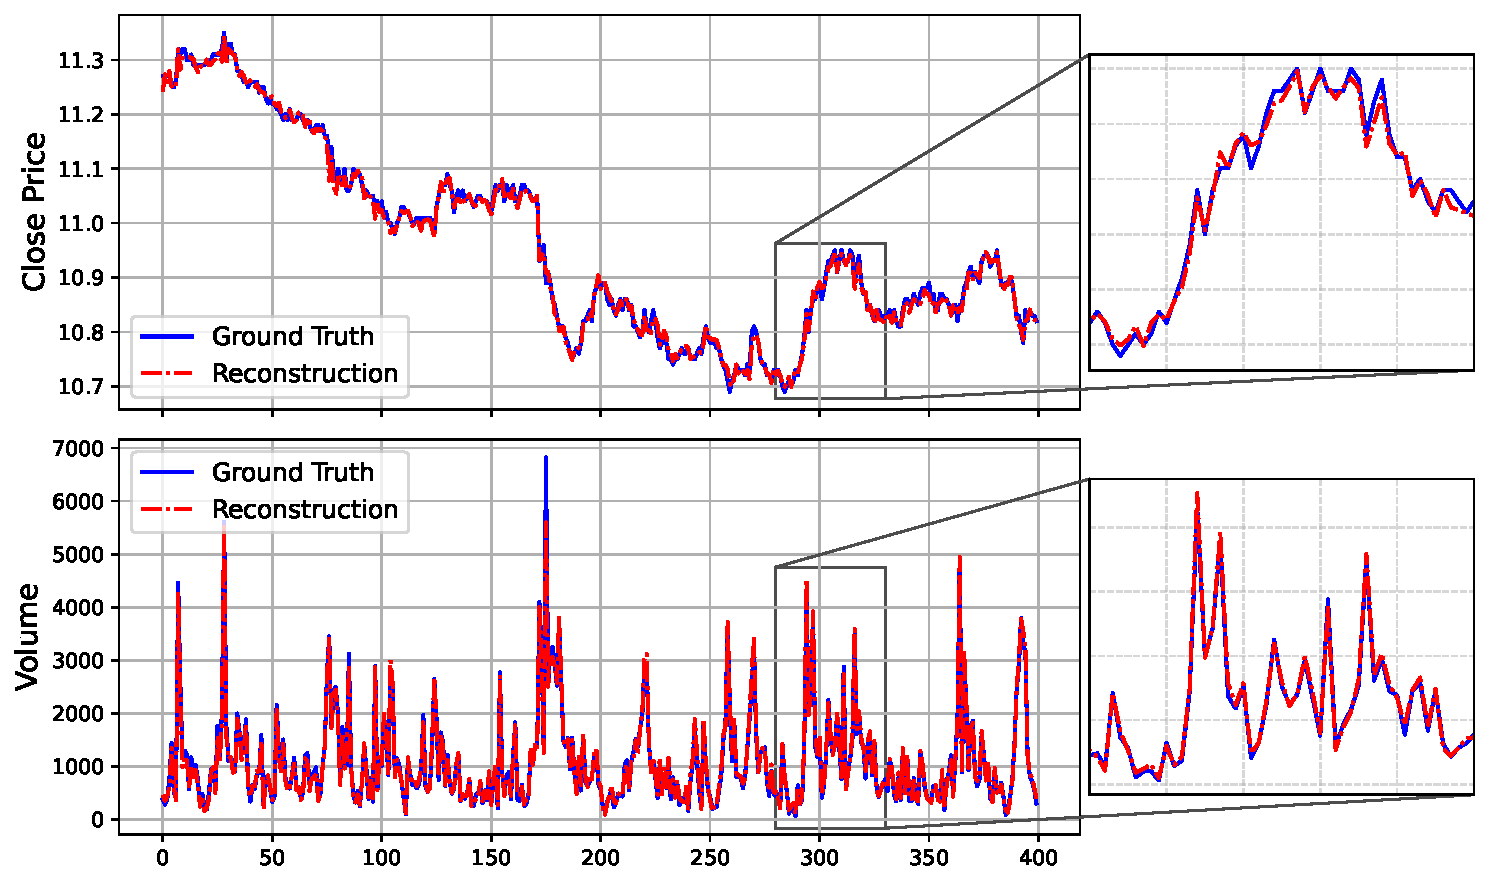
\includegraphics[width=\linewidth]{recon_imgs/pred_visualize_stock_XSHG_600977_5min.pdf}
        \caption{China Film Co.,Ltd. (SSE: 600977)}
    \end{subfigure}
    \hfill
    \begin{subfigure}[b]{0.49\textwidth}
        \centering
        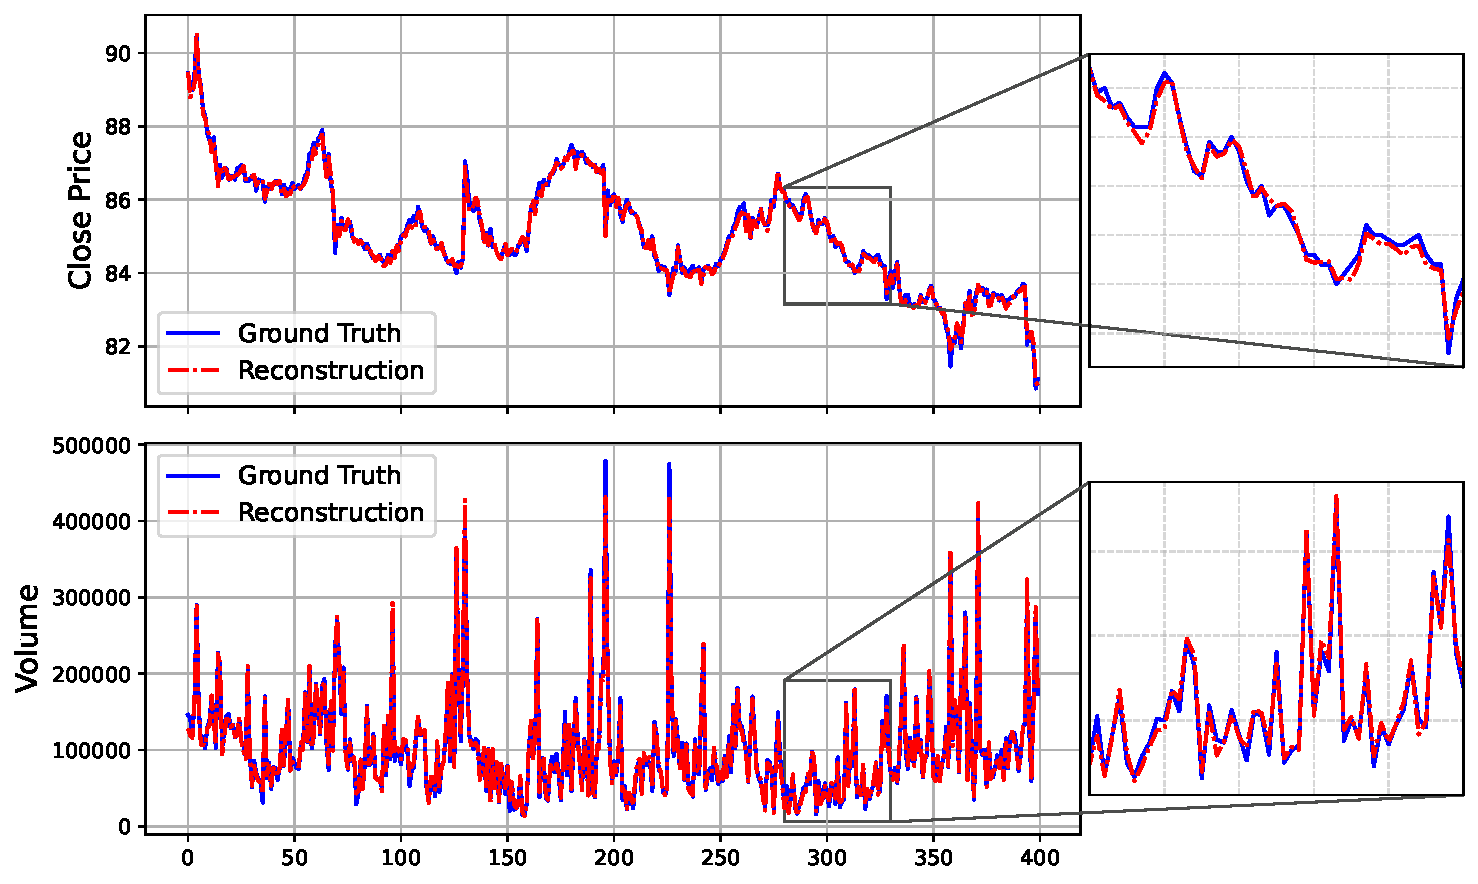
\includegraphics[width=\linewidth]{recon_imgs/pred_visualize_stock_XHKG_9992_5min.pdf}
        \caption{Pop Mart (HKEX: 09992)}
    \end{subfigure}

    \vspace{0.1cm}

    \begin{subfigure}[b]{0.49\textwidth}
        \centering
        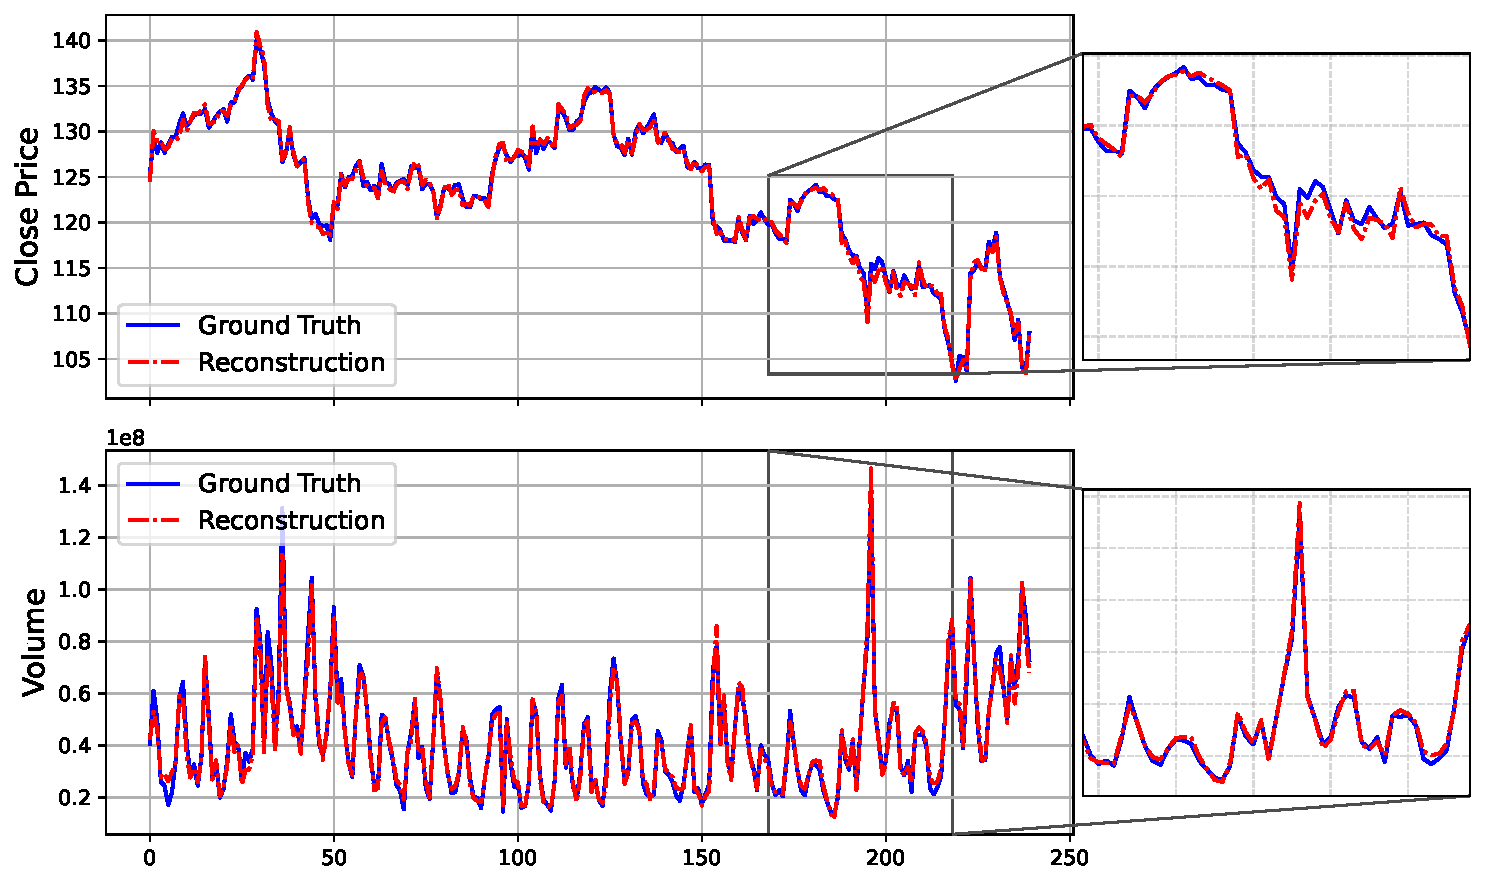
\includegraphics[width=\linewidth]{recon_imgs/pred_visualize_stock_XNAS_NVDA_60min.pdf}
        \caption{NVIDIA (NASDAQ: NVDA)}
    \end{subfigure}
    \hfill
    \begin{subfigure}[b]{0.49\textwidth}
        \centering
        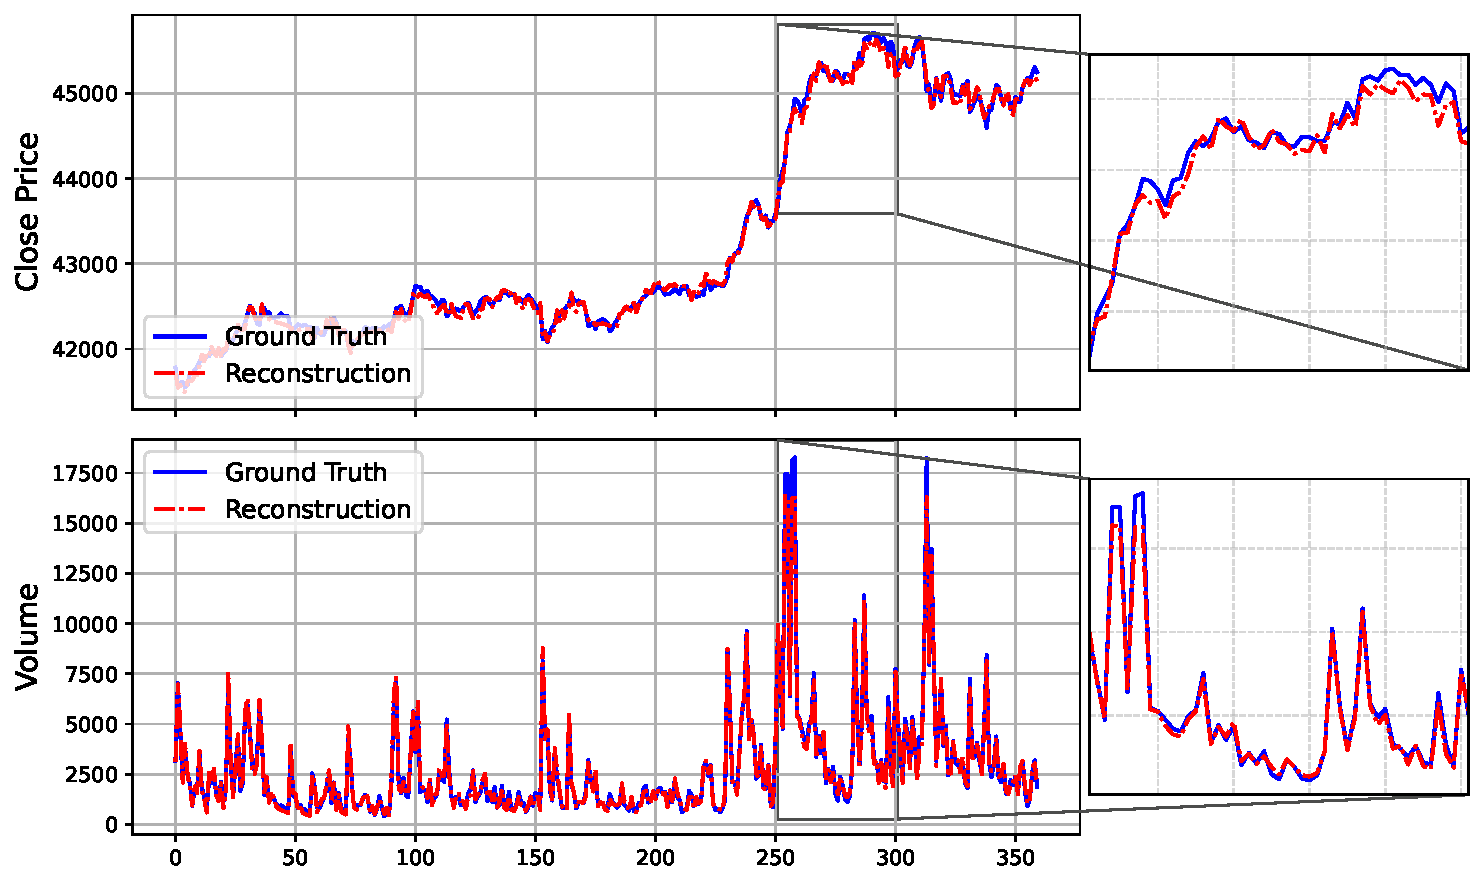
\includegraphics[width=\linewidth]{recon_imgs/pred_visualize_crypto_BTCUSDT_15min.pdf}
        \caption{BTC/USDT 무기한 (Binance: BTCUSDT)}
    \end{subfigure}

    \vspace{0.1cm}

    \begin{subfigure}[b]{0.49\textwidth}
        \centering
        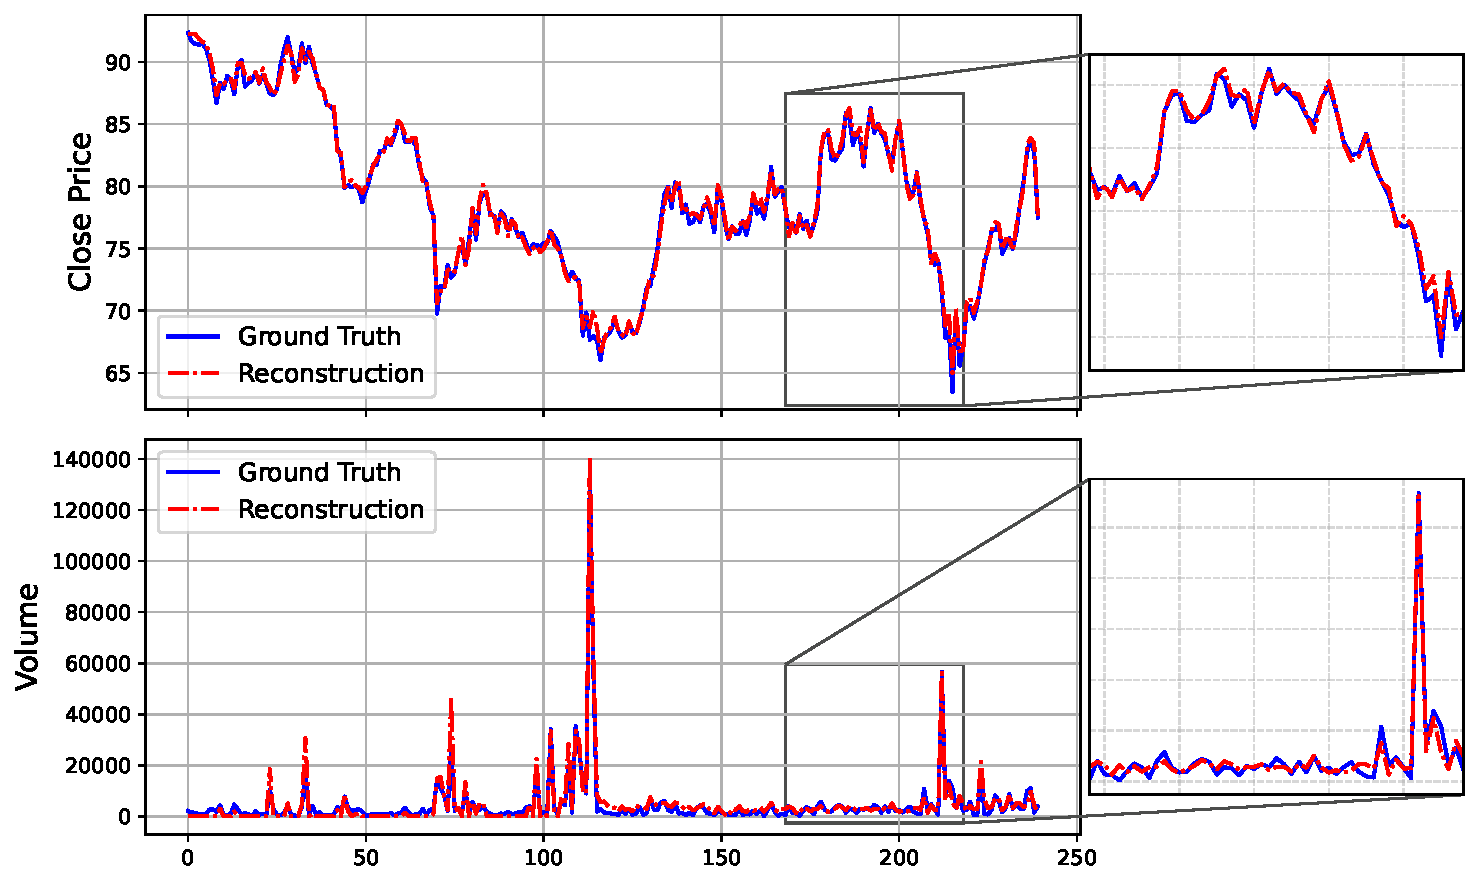
\includegraphics[width=\linewidth]{recon_imgs/pred_visualize_stock_XFRA_BMW_daily.pdf}
        \caption{BMW (FWB: BMW)}
    \end{subfigure}
    \hfill
    \begin{subfigure}[b]{0.49\textwidth}
        \centering
        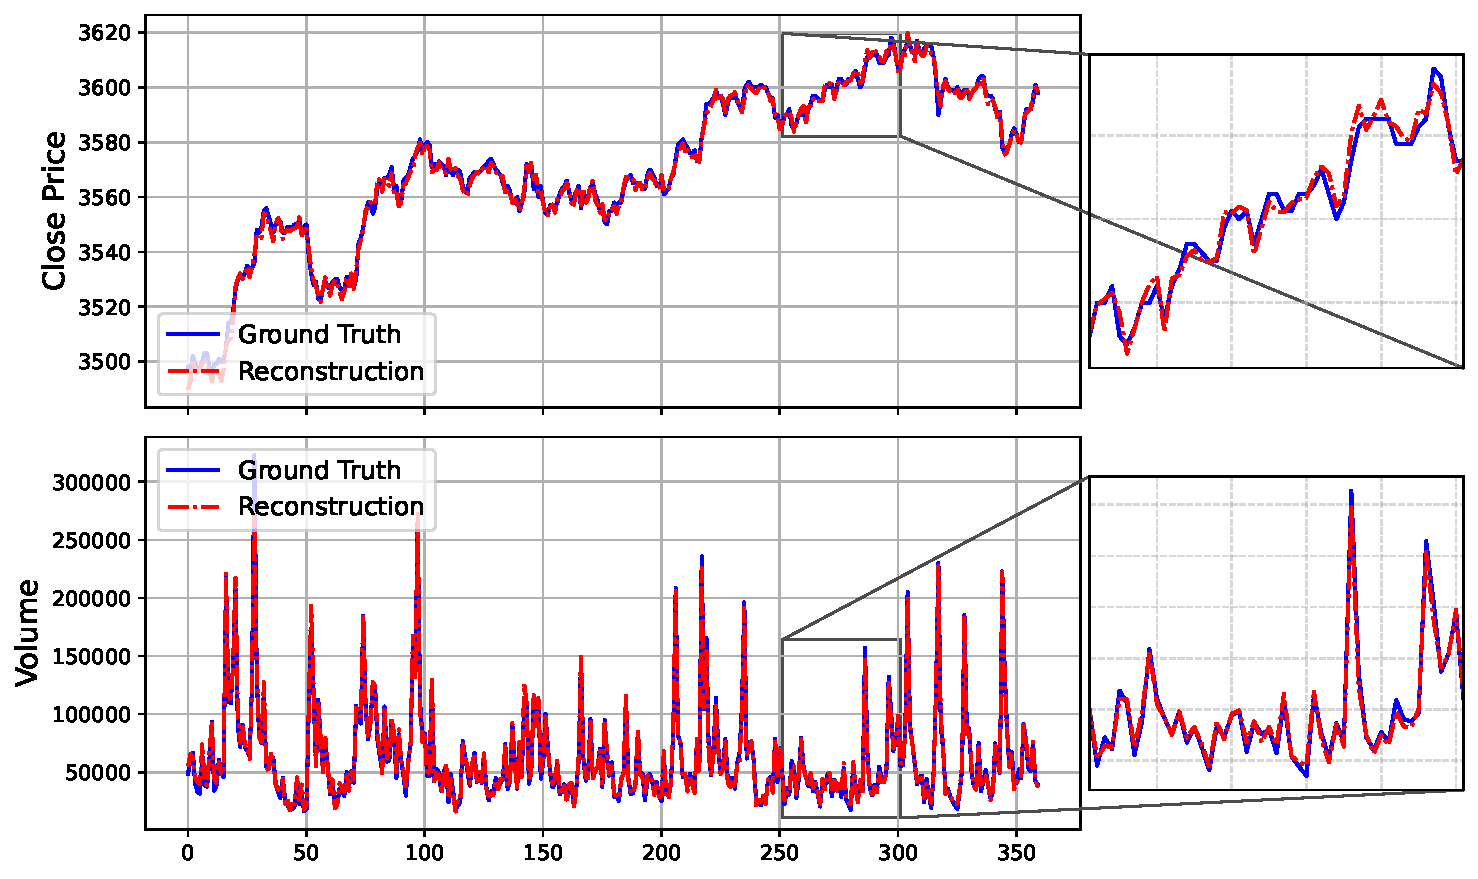
\includegraphics[width=\linewidth]{recon_imgs/pred_visualize_commodity_RB_5min.pdf}
        \caption{철근 선물 (SHFE: RB)}
    \end{subfigure}

    \vspace{0.1cm}

    \caption{K-line Tokenizer가 생성한 `Close Price'와 `Volume'의 재구성 결과 시각화. \textcolor{blue}{Blue} 선은 정답값을 나타내며, \textcolor{red}{red} 선은 우리 모델이 생성한 재구성 결과를 나타낸다.}
    \label{fig:recon_case}
\end{figure*}




\begin{figure*}[htbp]
    \centering

    \begin{subfigure}{\textwidth}
        \centering
        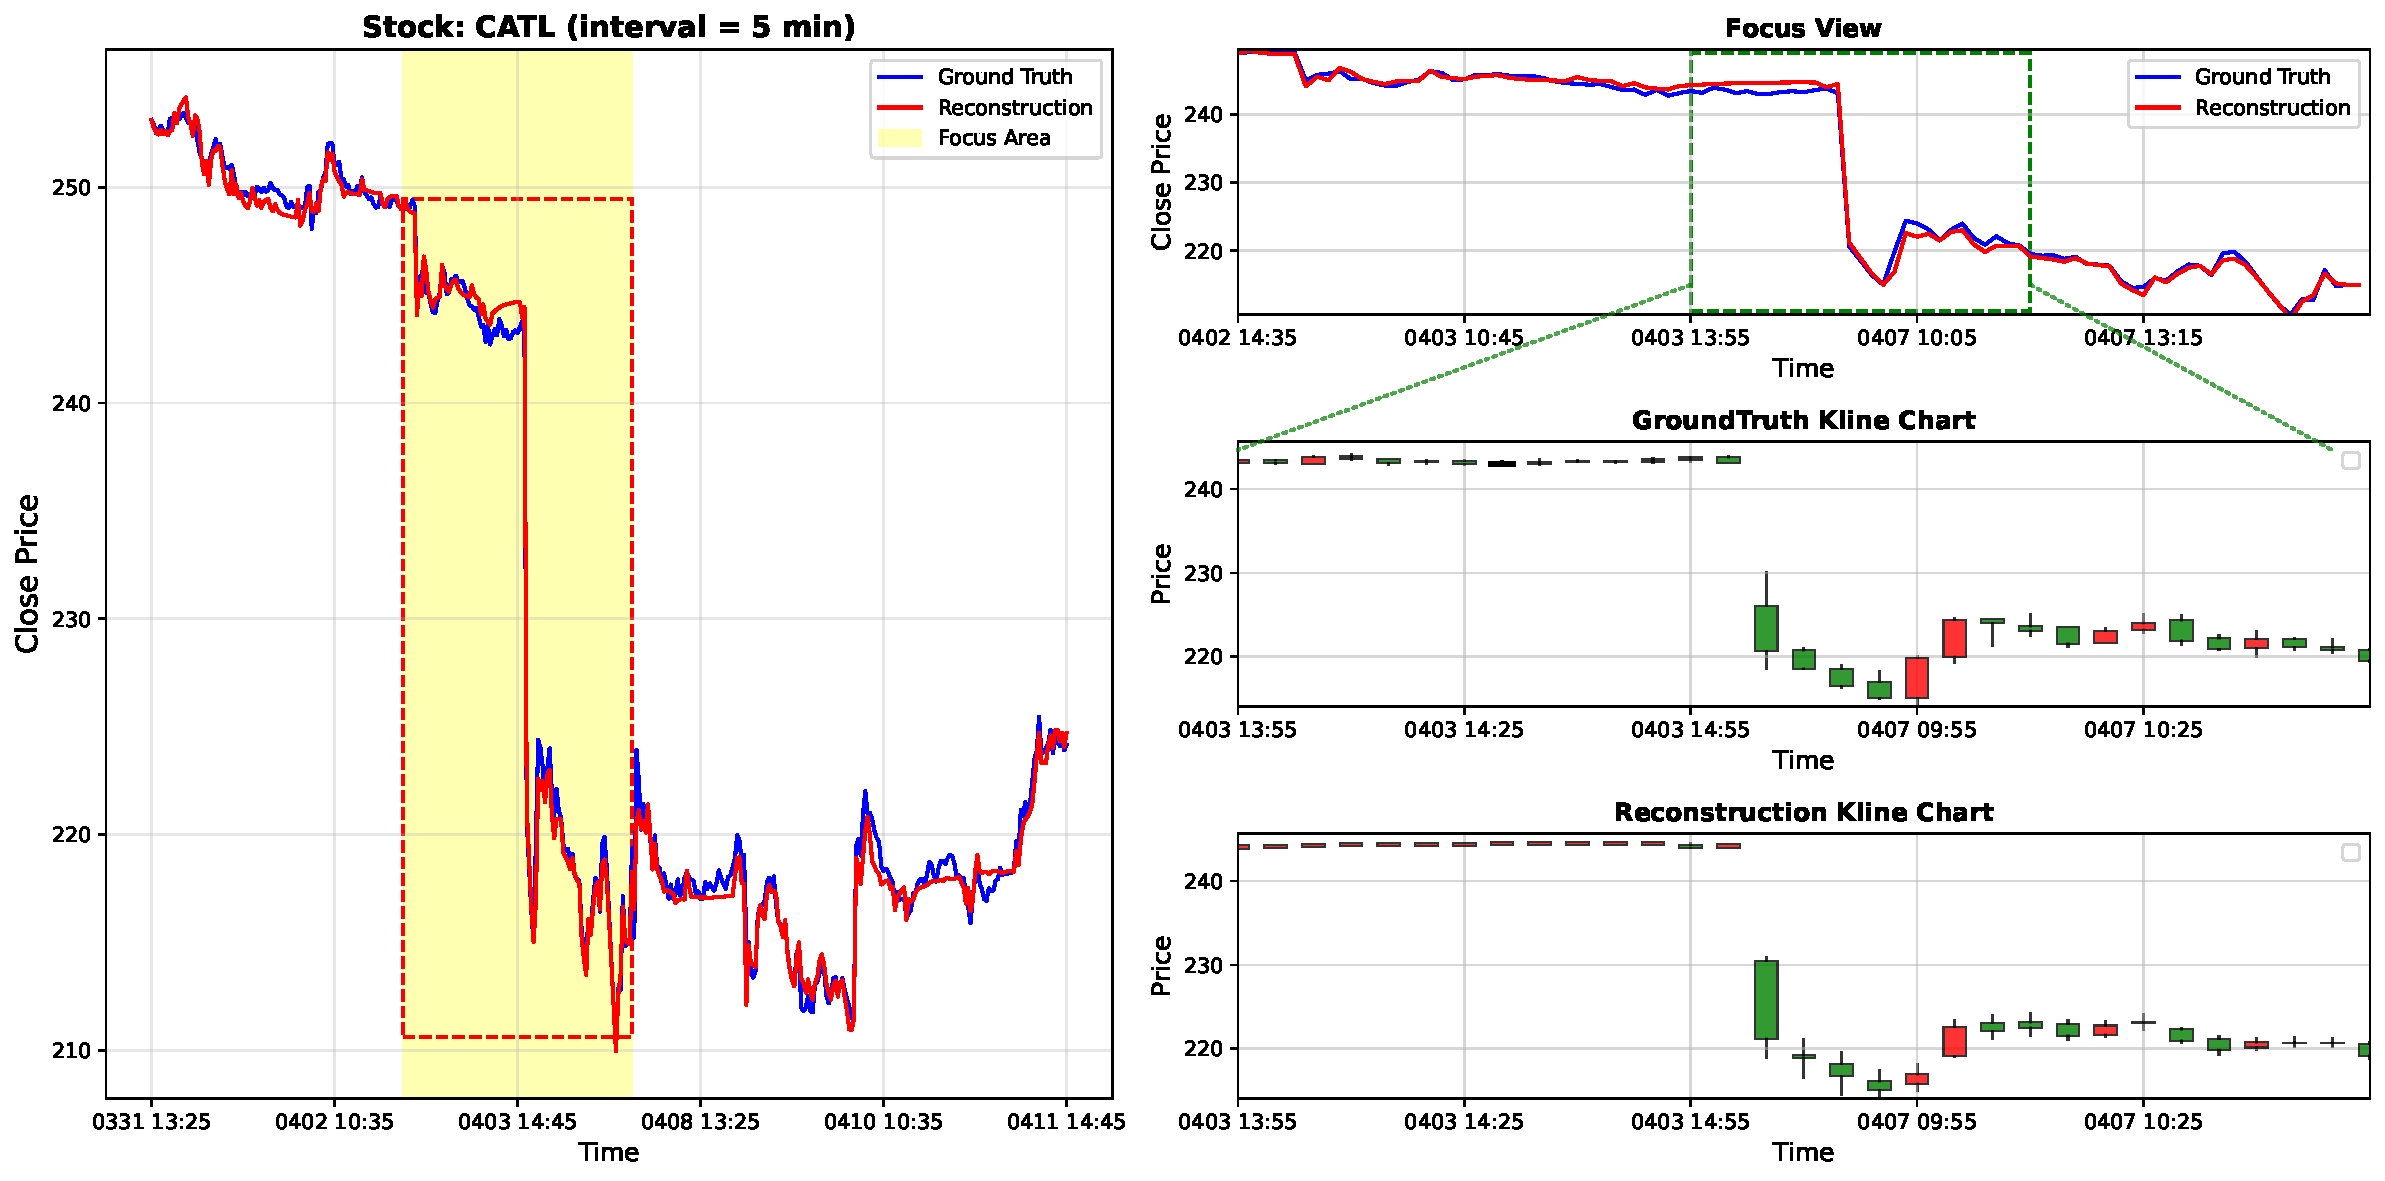
\includegraphics[width=1.0\textwidth]{recon_imgs/cn_300750_5min_shocks_price_release.pdf}
        \caption{주식 K-line 재구성, 가격 부분 }
    \end{subfigure}

    \begin{subfigure}{\textwidth}
        \centering
        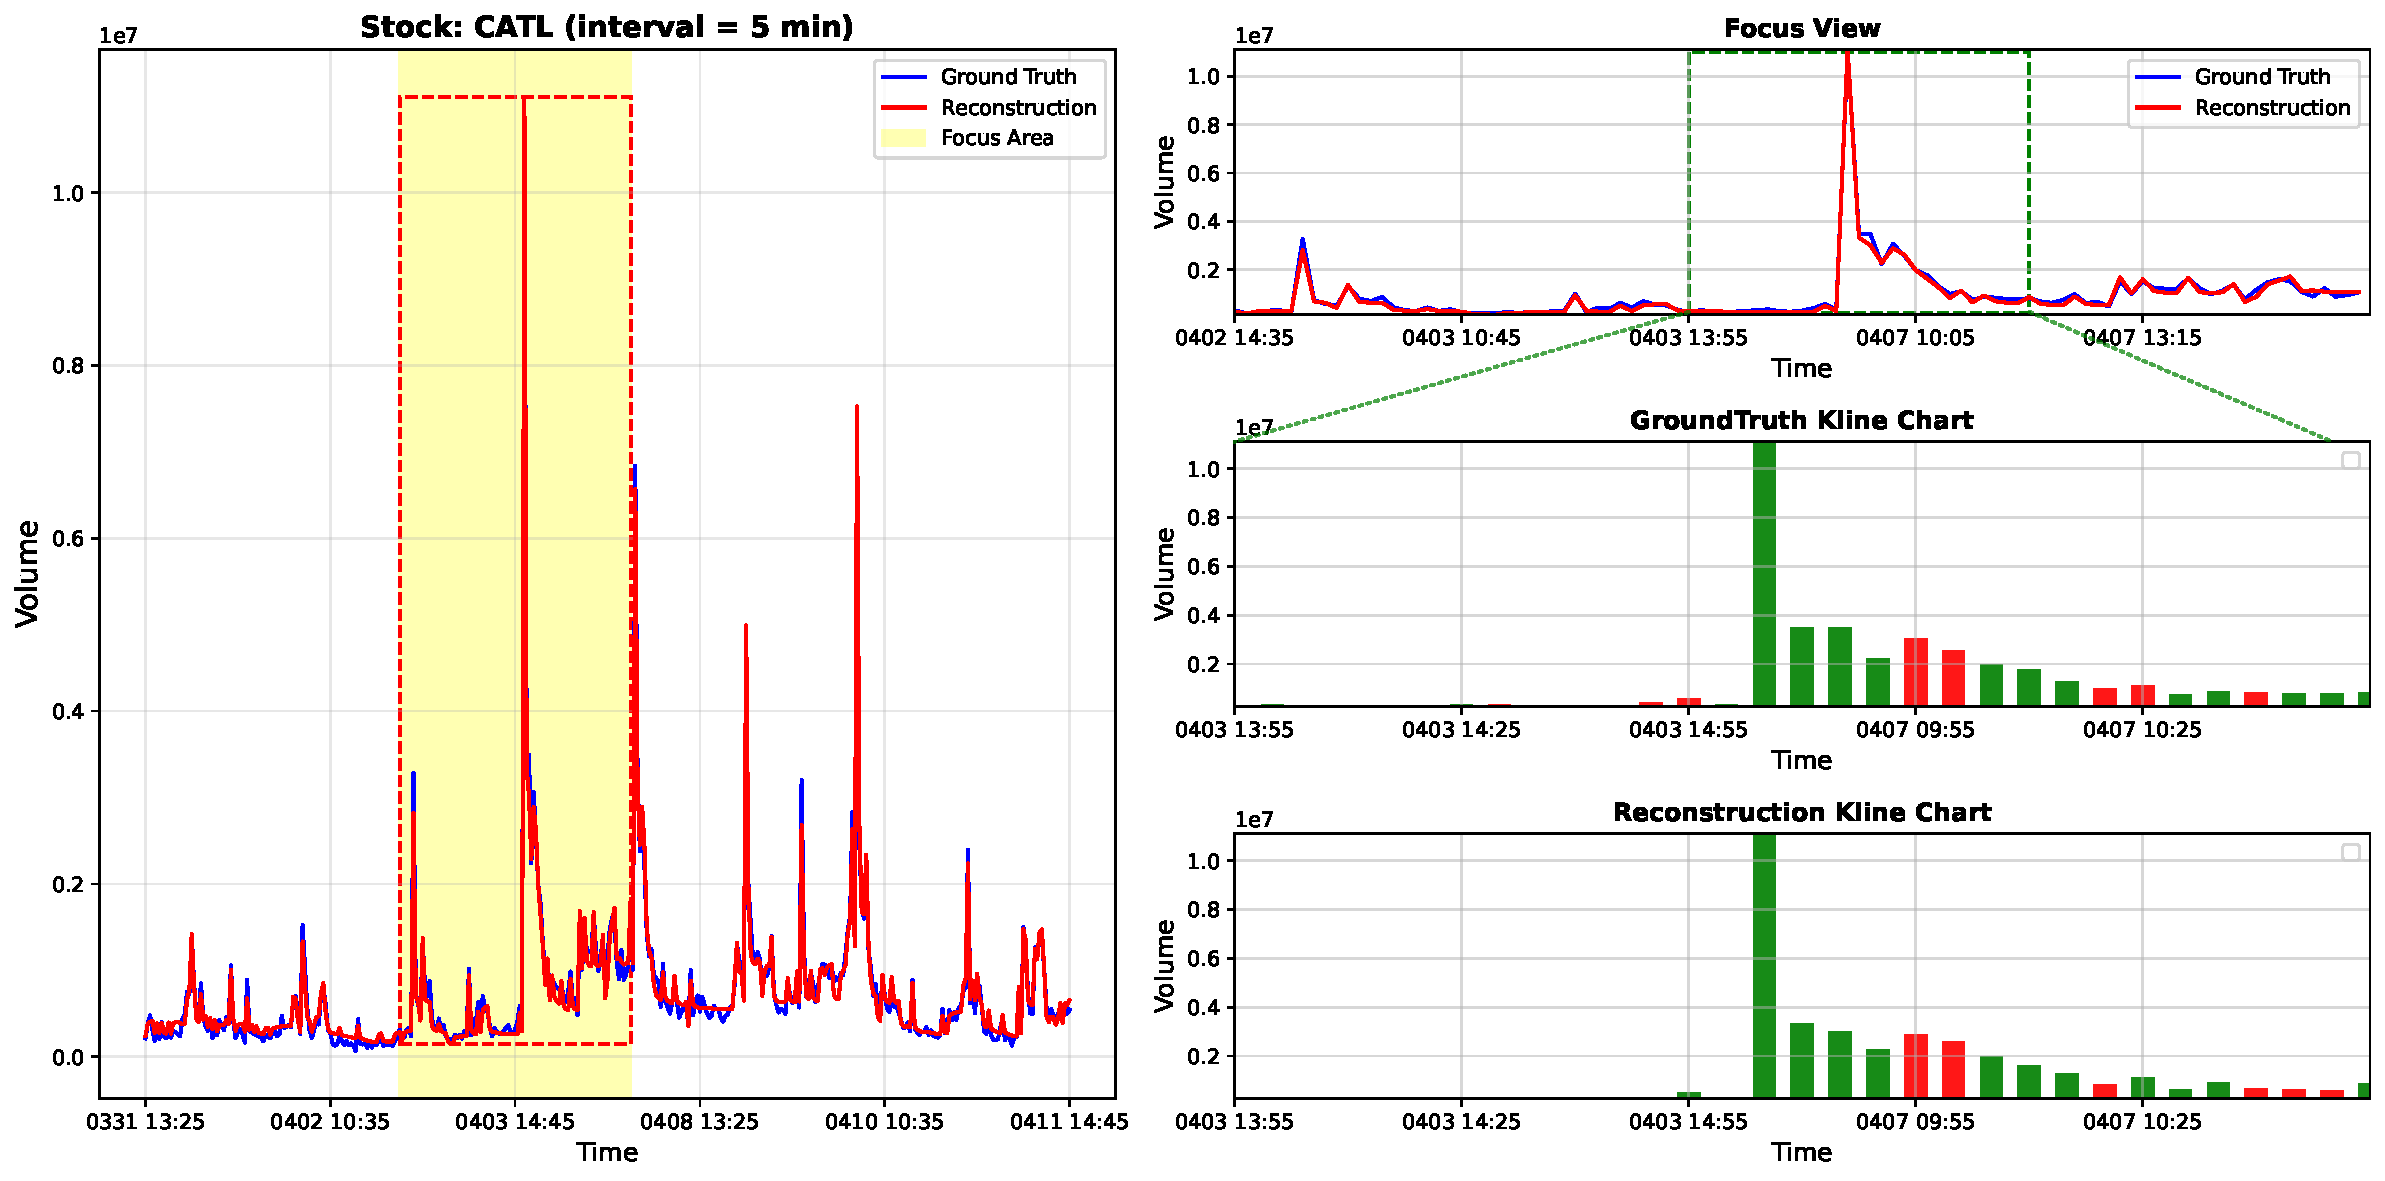
\includegraphics[width=1.0\textwidth]{recon_imgs/cn_300750_5min_shocks_volume_release.pdf}
        \caption{주식 K-line 재구성, 거래량 부분}
    \end{subfigure}

    \vspace{0.1cm}


    \caption{
    Trump의 무역전쟁~\cite{mckibbin2025global}이라는 경제적 맥락에서 2025년 4월 7일 CATL (Contemporary Amperex Technology Co., Limited)의 5분 K-line 데이터 재구성 성능을 보여 주는 예시. 시각화에서 캔들스틱은 ``상승은 빨간색, 하락은 초록색'' 관례를 따르며(상승/하락은 시가 대비 종가로 결정됨), 거래량 막대도 이에 맞추어 색칠된다.
    }
    \label{fig:kline_reconstruction_tradewar}
\end{figure*}







\twocolumn

% \begin{figure*}[ht]
%     \centering

%     \begin{subfigure}[b]{0.32\textwidth}
%         \centering
%         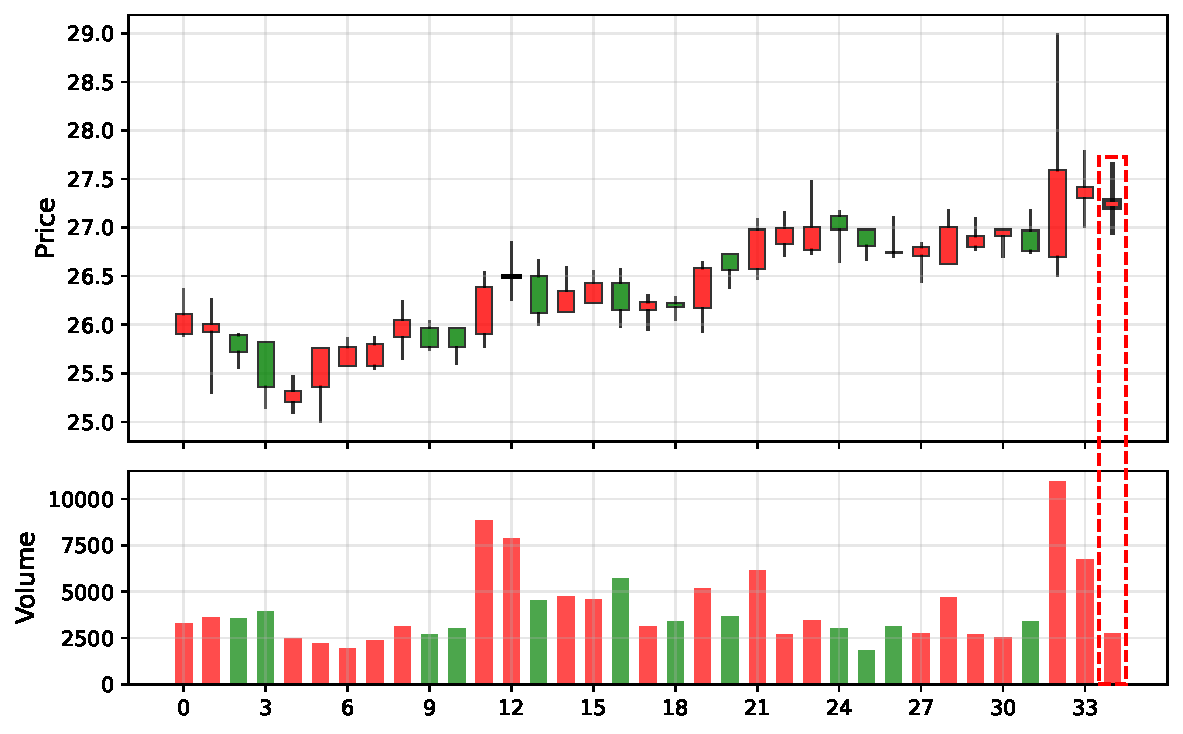
\includegraphics[width=\linewidth]{tokens/high_used_token_1.pdf}
%         \caption{빈도가 높은 토큰 예시 1}
%     \end{subfigure}
%     \hfill
%     \begin{subfigure}[b]{0.32\textwidth}
%         \centering
%         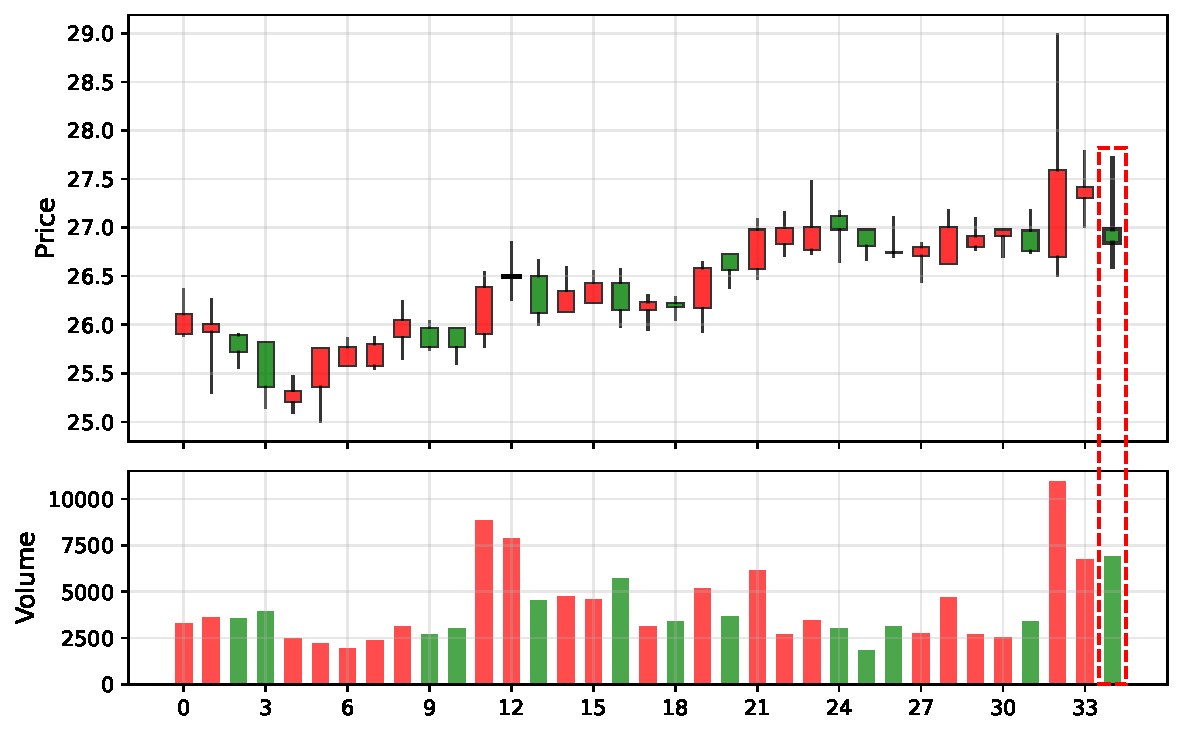
\includegraphics[width=\linewidth]{tokens/high_used_token_2.pdf}
%         \caption{빈도가 높은 토큰 예시 2}
%     \end{subfigure}
%     \hfill
%     \begin{subfigure}[b]{0.32\textwidth}
%         \centering
%         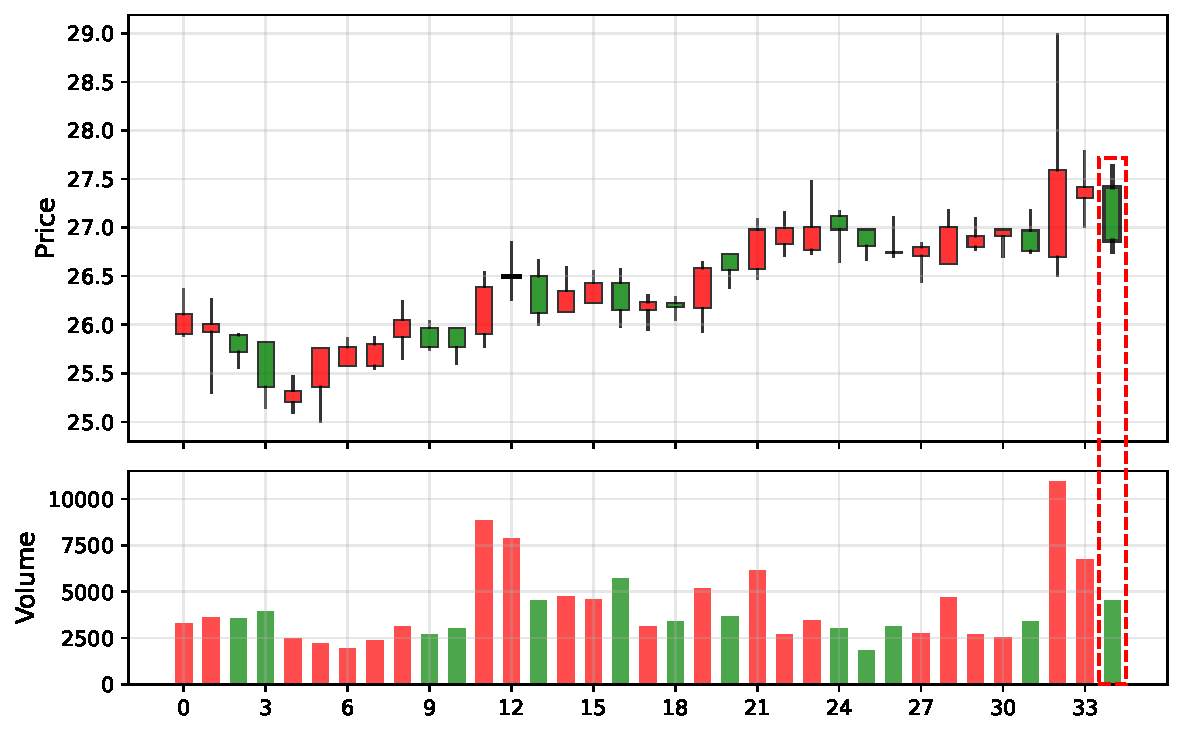
\includegraphics[width=\linewidth]{tokens/high_used_token_3.pdf}
%         \caption{빈도가 높은 토큰 예시 3}
%     \end{subfigure}

%     \vspace{0.1cm}

%     \begin{subfigure}[b]{0.32\textwidth}
%         \centering
%         \includegraphics[width=\linewidth]{tokens/low_usage_token_1.pdf}
%         \caption{빈도가 낮은 토큰 예시 1}
%     \end{subfigure}
%     \hfill
%     \begin{subfigure}[b]{0.32\textwidth}
%         \centering
%         \includegraphics[width=\linewidth]{tokens/low_usage_token_2.pdf}
%         \caption{빈도가 낮은 토큰 예시 2}
%     \end{subfigure}
%     \hfill
%     \begin{subfigure}[b]{0.32\textwidth}
%         \centering
%         \includegraphics[width=\linewidth]{tokens/low_usage_token_3.pdf}
%         \caption{빈도가 낮은 토큰 예시 3}
%     \end{subfigure}

%     \vspace{0.1cm}

%     \begin{subfigure}[b]{0.32\textwidth}
%         \centering
%         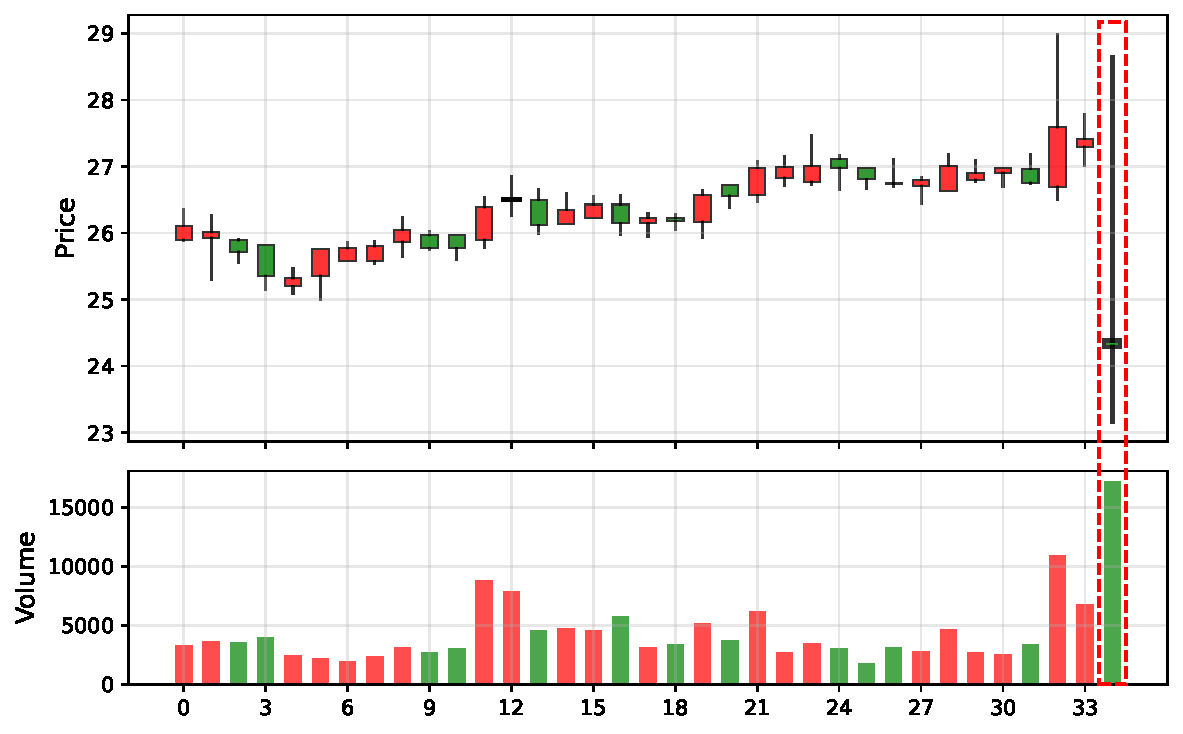
\includegraphics[width=\linewidth]{tokens/unused_token_1.pdf}
%         \caption{사용되지 않은 토큰 예시 1}
%     \end{subfigure}
%     \hfill
%     \begin{subfigure}[b]{0.32\textwidth}
%         \centering
%         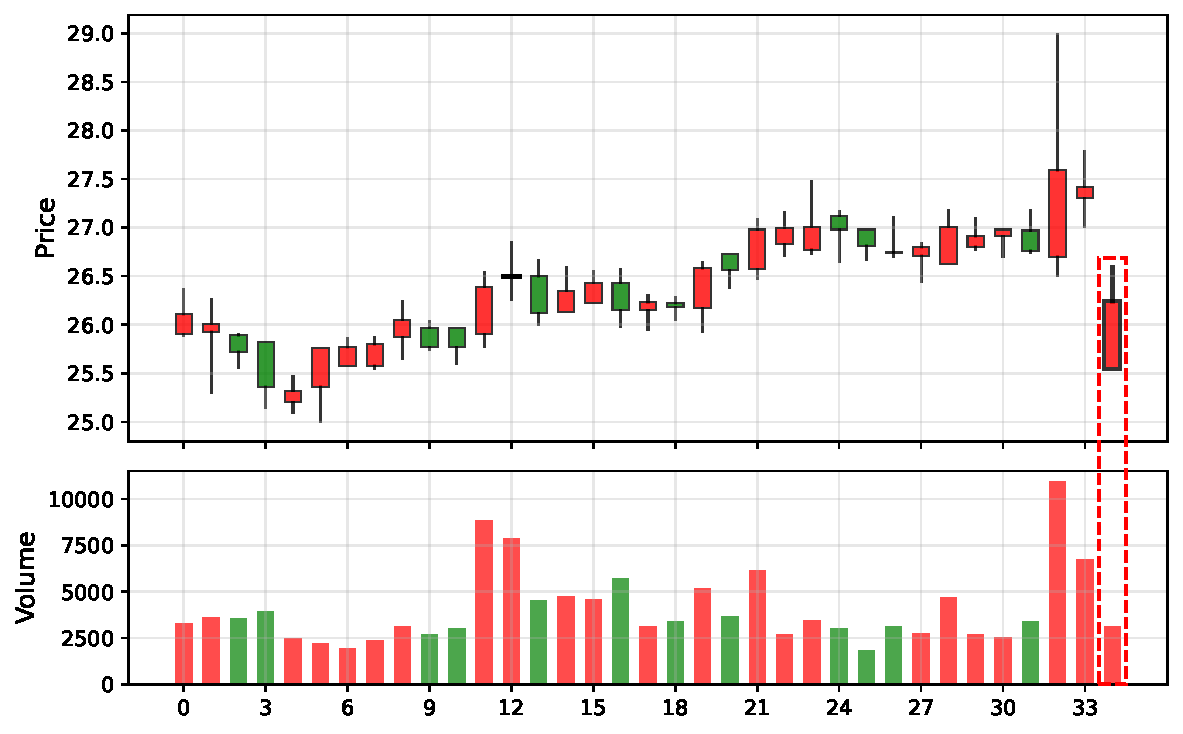
\includegraphics[width=\linewidth]{tokens/unused_token_2.pdf}
%         \caption{사용되지 않은 토큰 예시 2}
%     \end{subfigure}
%     \hfill
%     \begin{subfigure}[b]{0.32\textwidth}
%         \centering
%         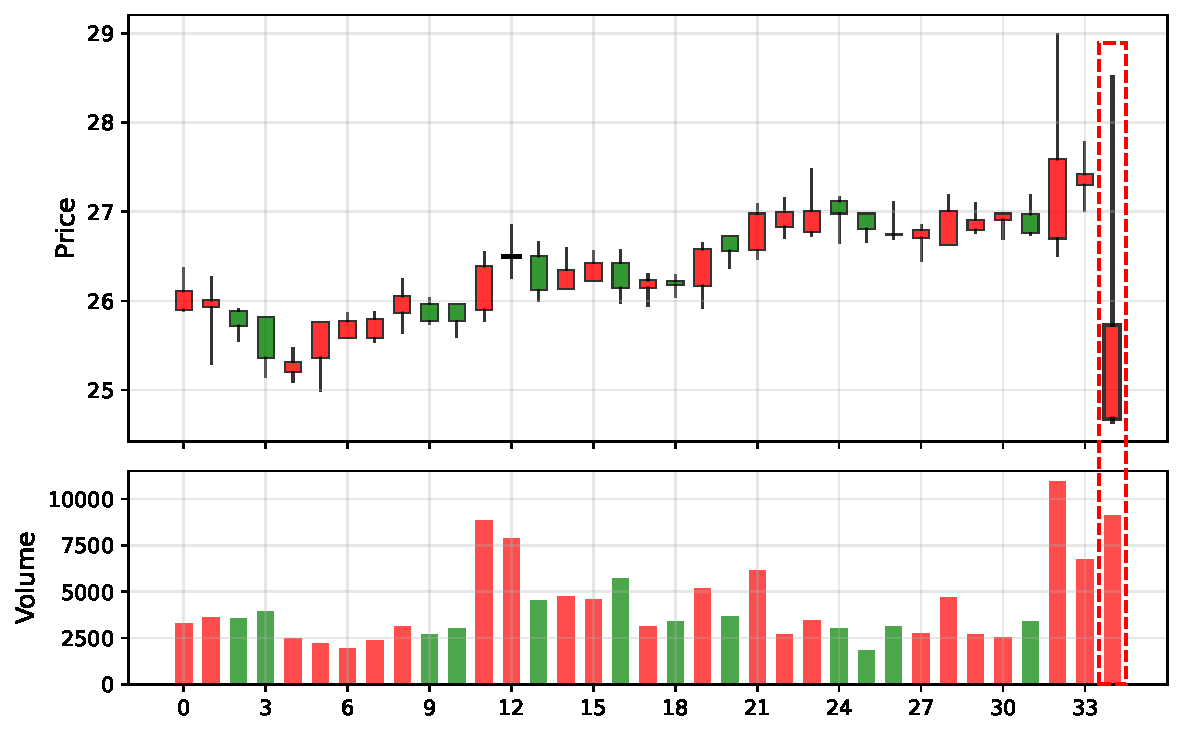
\includegraphics[width=\linewidth]{tokens/unused_token_3.pdf}
%         \caption{사용되지 않은 토큰 예시 3}
%     \end{subfigure}
%     \vspace{0.1cm}


%     \begin{subfigure}[b]{0.32\textwidth}
%         \centering
%         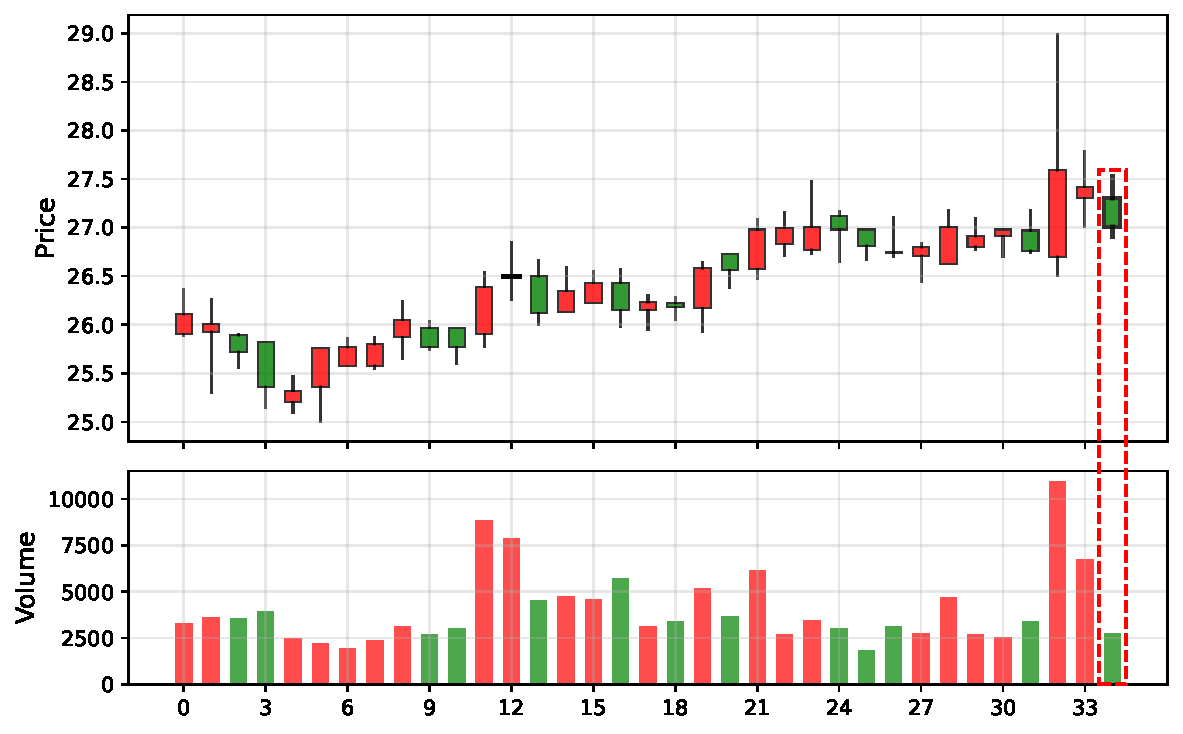
\includegraphics[width=\linewidth]{tokens/original_kline.pdf}
%         \caption{원본 토큰 시퀀스 샘플}
%     \end{subfigure}


%     \caption{토큰 예시}
%     \label{fig:token_show_case}
% \end{figure*}



\begin{figure*}[ht]
    \centering

    % 그룹 1: 고빈도 토큰
    \begin{subfigure}[b]{\textwidth}
        \centering
        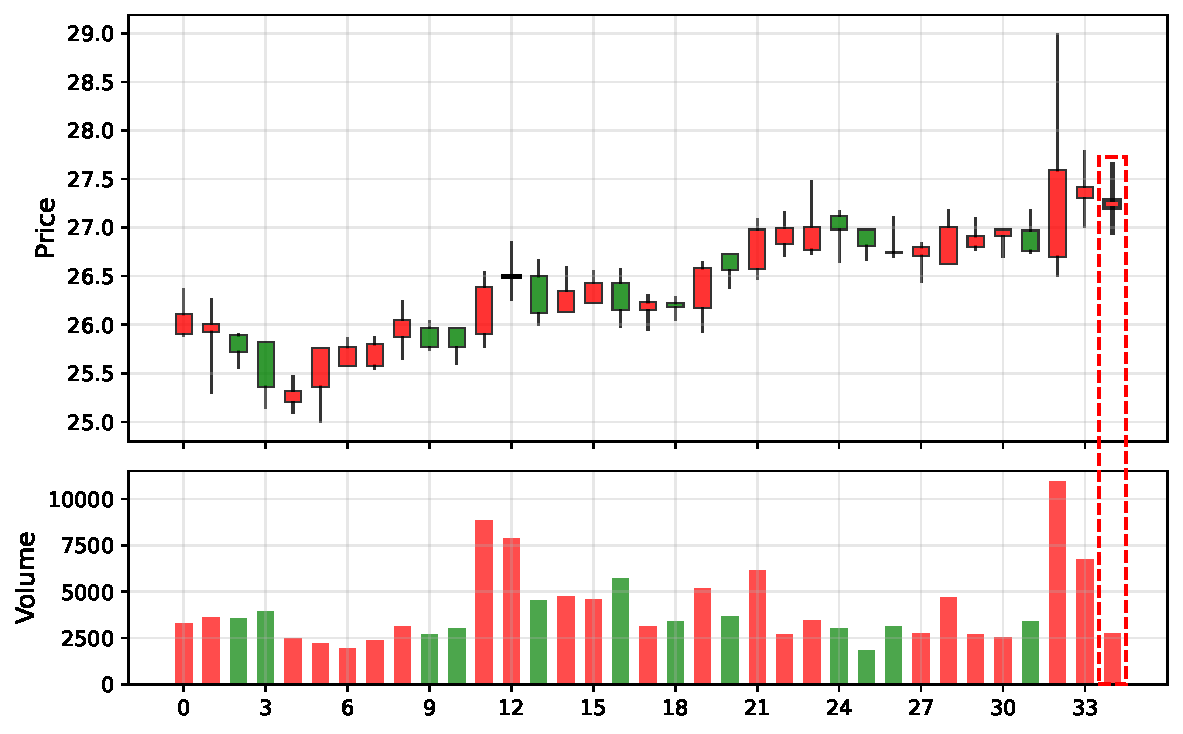
\includegraphics[width=0.32\textwidth]{tokens/high_used_token_1.pdf}
        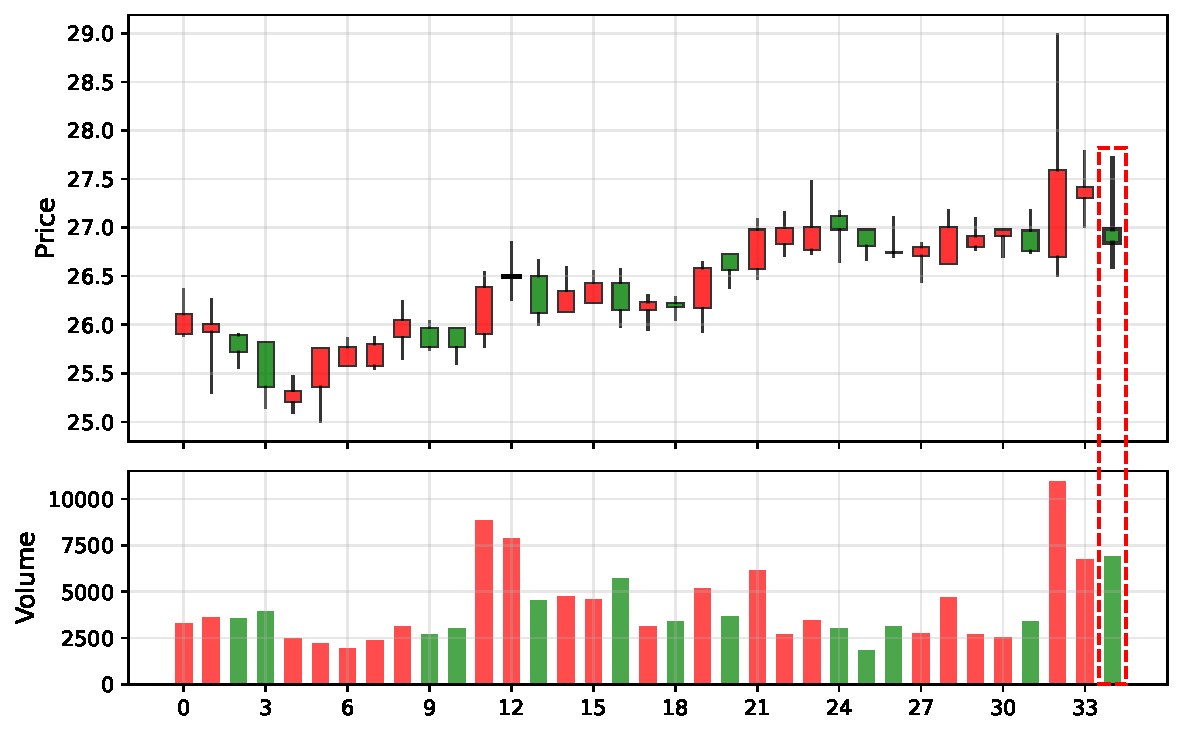
\includegraphics[width=0.32\textwidth]{tokens/high_used_token_2.pdf}
        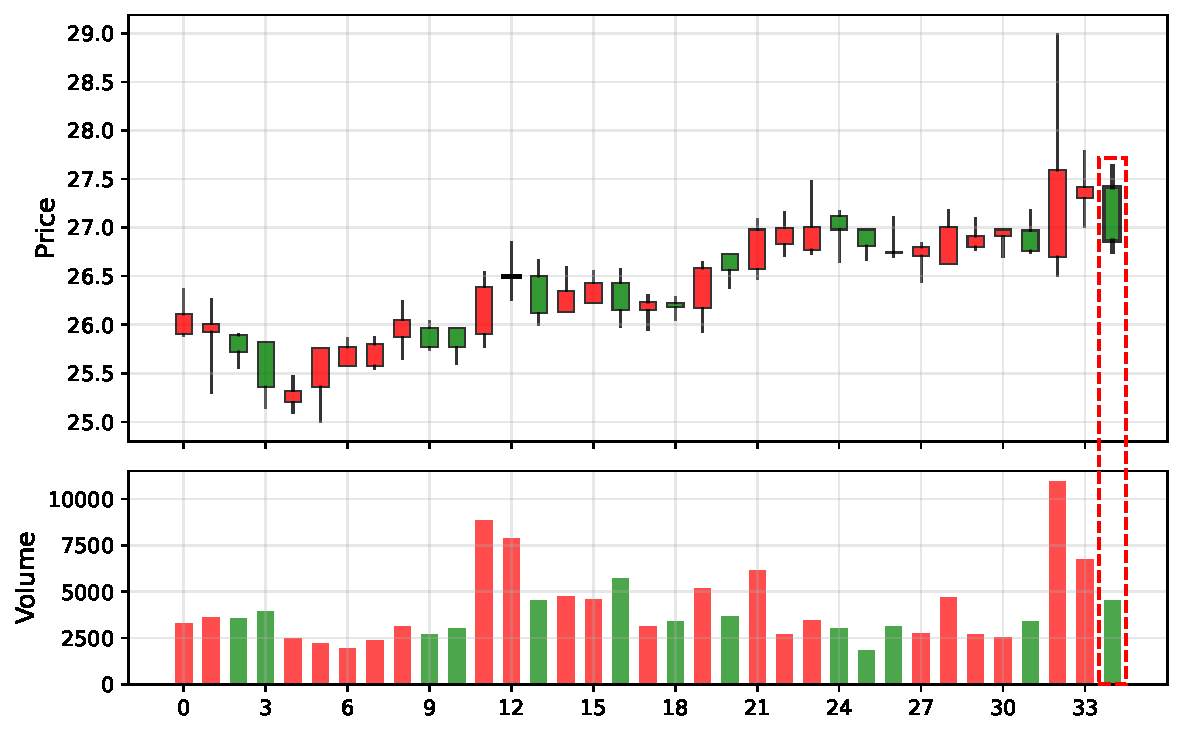
\includegraphics[width=0.32\textwidth]{tokens/high_used_token_3.pdf}
        \caption{고빈도 토큰의 예시.}
    \end{subfigure}
    \vspace{0.1cm}

    % 그룹 2: 저빈도 토큰
    \begin{subfigure}[b]{\textwidth}
        \centering
        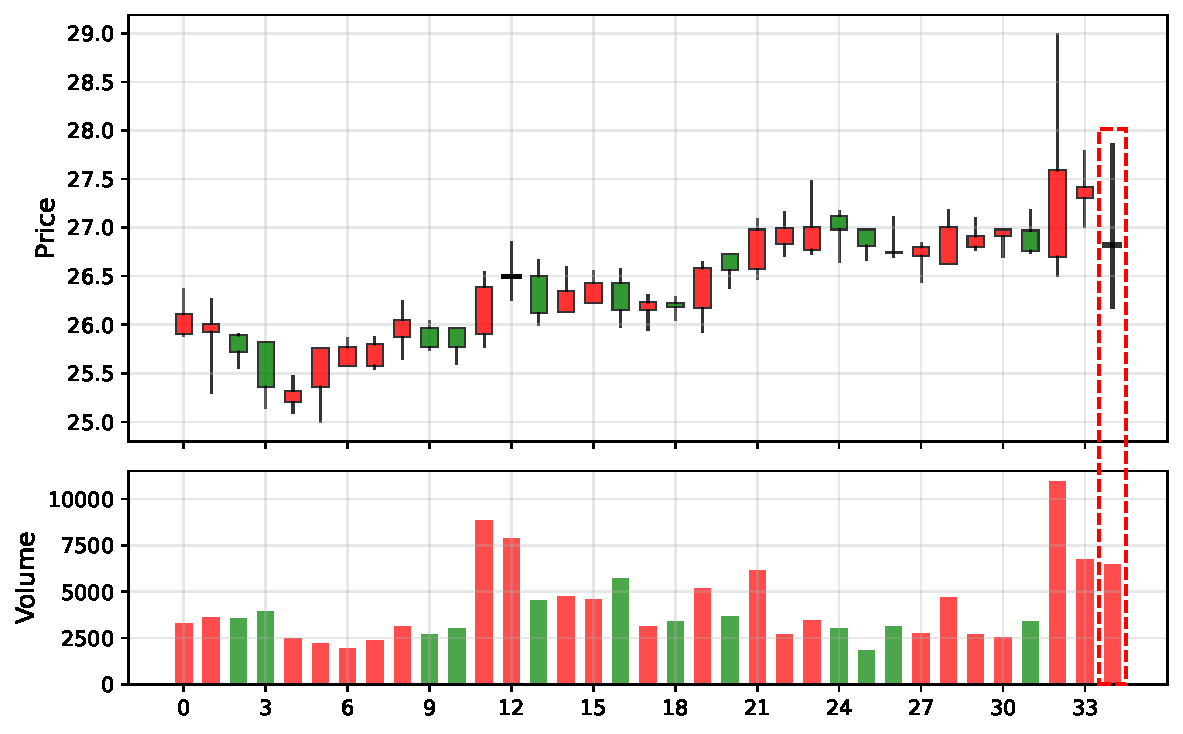
\includegraphics[width=0.32\textwidth]{tokens/low_used_token_1.pdf}
        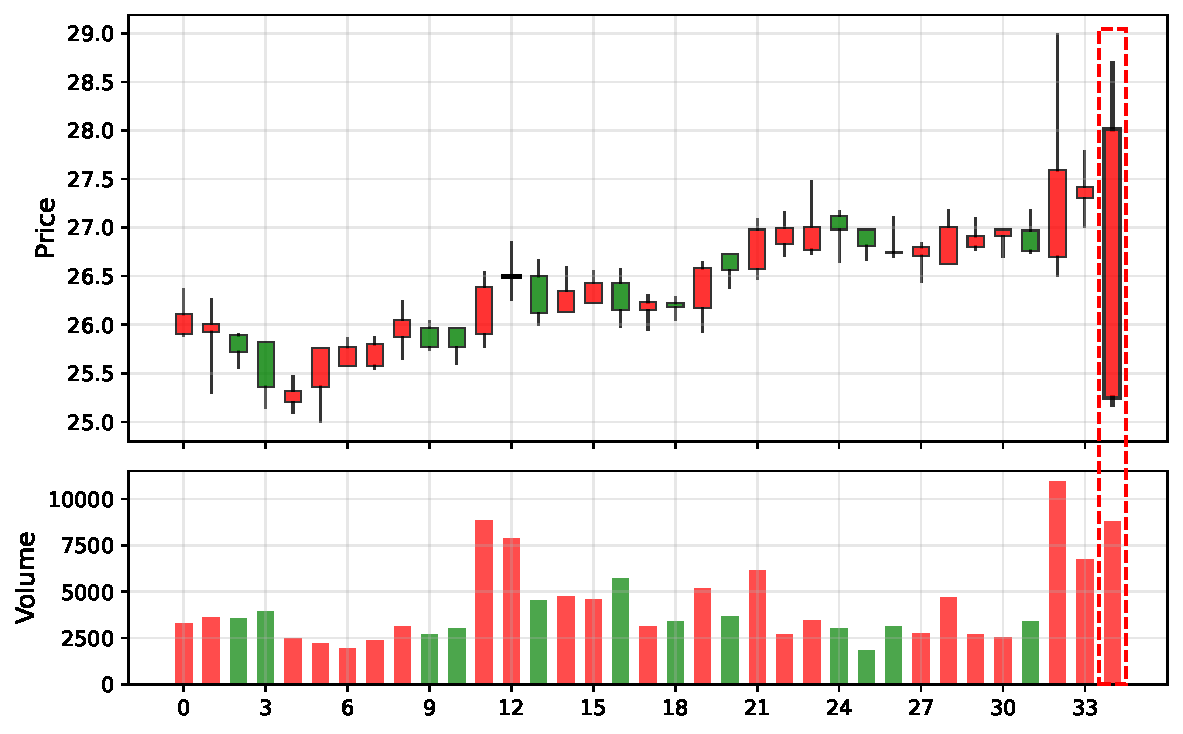
\includegraphics[width=0.32\textwidth]{tokens/low_used_token_2.pdf}
        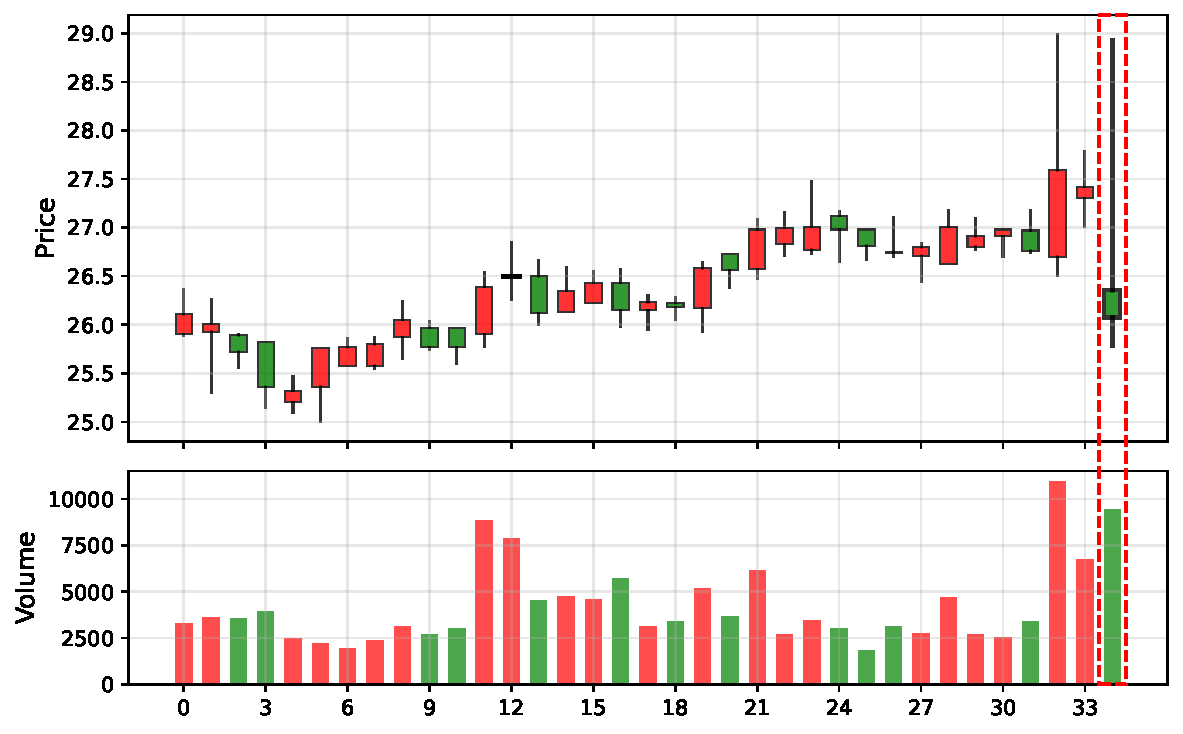
\includegraphics[width=0.32\textwidth]{tokens/low_used_token_3.pdf}
        \caption{저빈도 토큰의 예시.}
    \end{subfigure}
    \vspace{0.1cm}

    % 그룹 3: 사용되지 않은 토큰
    \begin{subfigure}[b]{\textwidth}
        \centering
        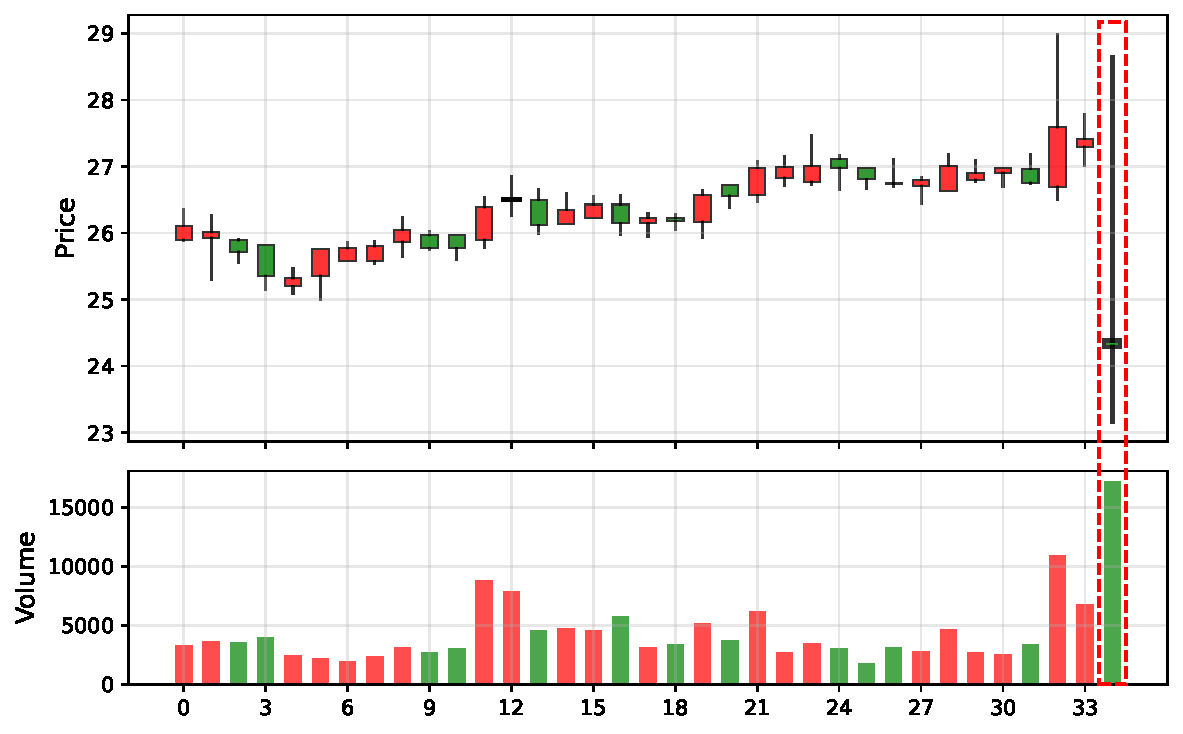
\includegraphics[width=0.32\textwidth]{tokens/unused_token_1.pdf}
        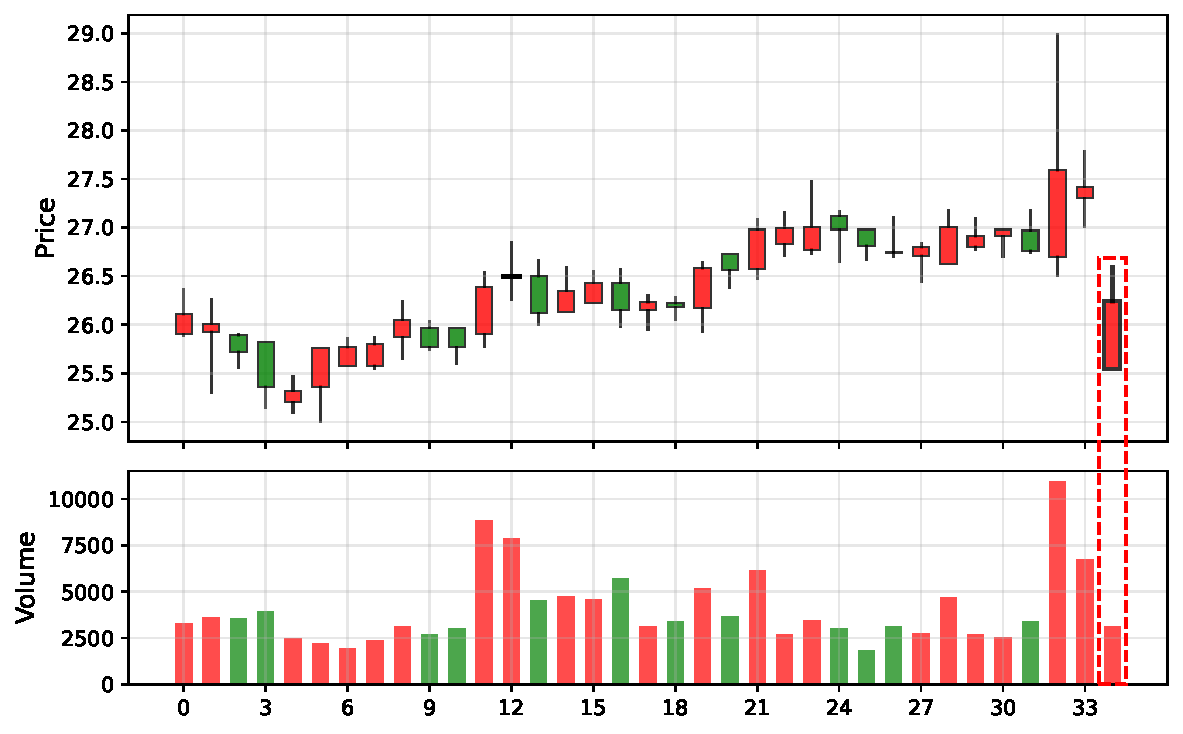
\includegraphics[width=0.32\textwidth]{tokens/unused_token_2.pdf}
        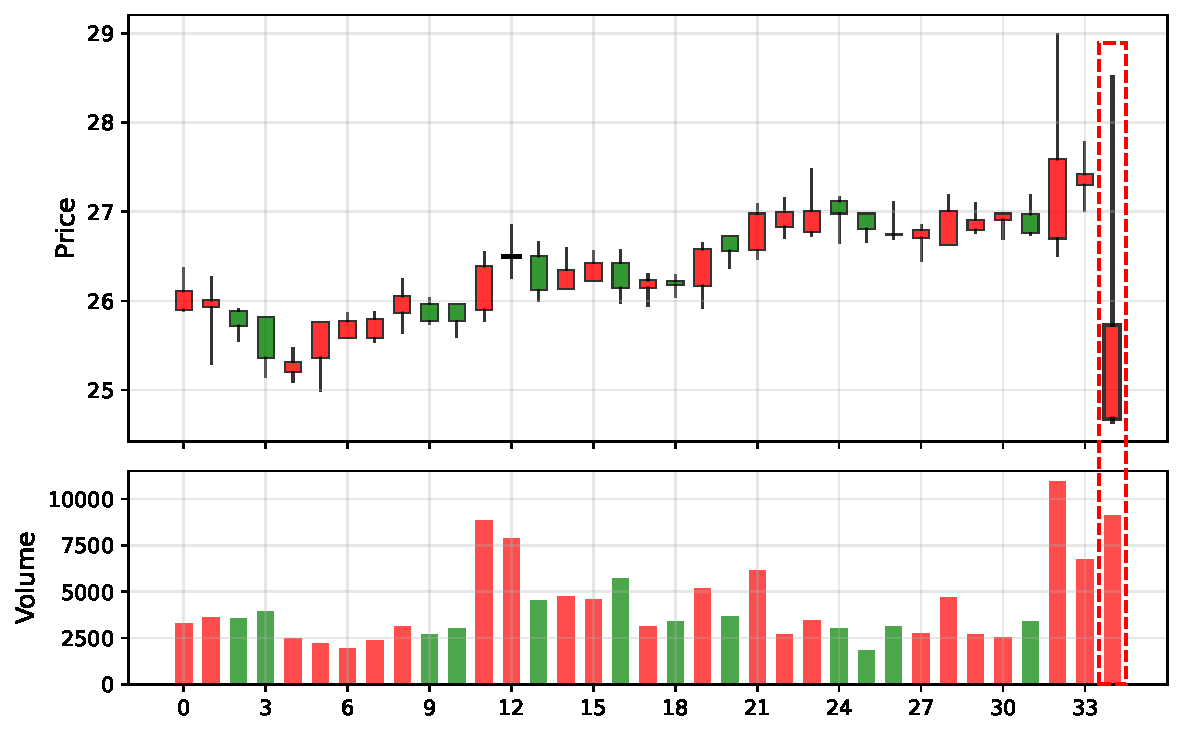
\includegraphics[width=0.32\textwidth]{tokens/unused_token_3.pdf}
        \caption{어휘집에서 사용되지 않은 토큰의 예시.}
    \end{subfigure}
    \vspace{0.1cm}

    % 그룹 4: 원본 토큰 시퀀스
    \begin{subfigure}[b]{\textwidth}
        \centering
        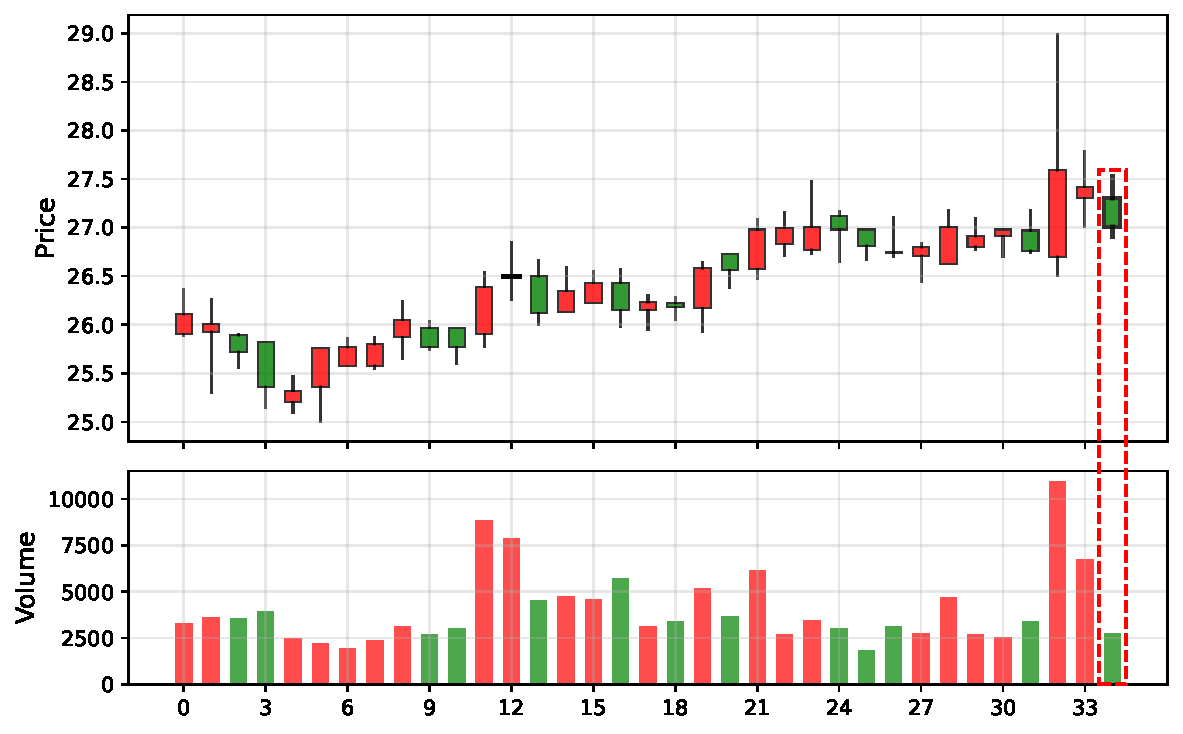
\includegraphics[width=0.32\textwidth]{tokens/original_kline.pdf}
        \caption{원본 토큰 시퀀스의 샘플.}
    \end{subfigure}

    \caption{토큰 사용 패턴의 시각화. 이 그림은 말뭉치에서의 출현 빈도를 기준으로 토큰 범주를 보여 준다: (a) 고빈도, (b) 저빈도, (c) 미사용(빈도 0) 토큰. 참고를 위해 원본 시퀀스 (d)의 샘플도 제시한다. (a), (b), (c)의 시퀀스는 (d)의 마지막 토큰을 해당 범주에서 무작위로 샘플링한 토큰으로 대체하여 구성하였다. 시각화에서 캔들스틱은 ``상승은 빨간색, 하락은 초록색'' 관례를 따르며(상승/하락은 시가 대비 종가로 결정됨), 거래량 막대도 이에 맞추어 색칠된다.}
    \label{fig:token_show_case}
\end{figure*}



\begin{figure*}[htbp]
    \centering

    \begin{subfigure}{\textwidth}
        \centering
        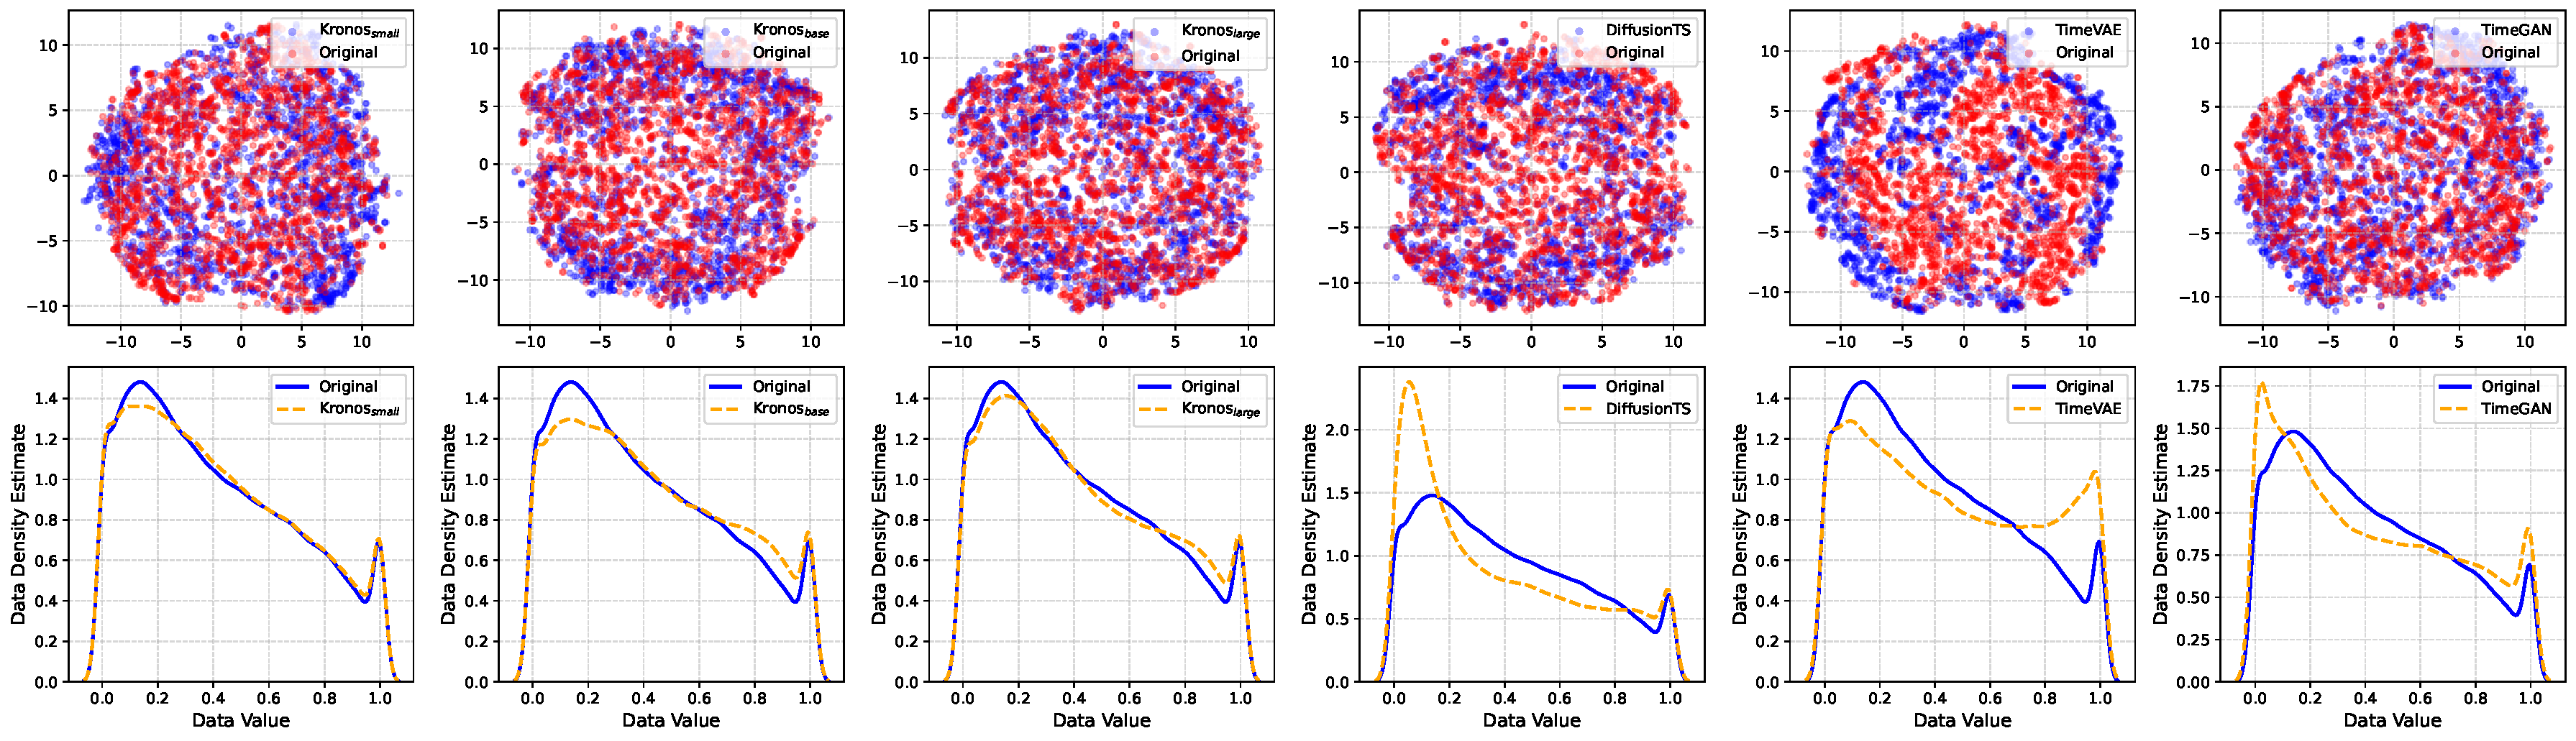
\includegraphics[width=1.0\textwidth]{img/gen_diversity_XSHG_daily.pdf}
        \caption{Shanghai Stock Exchange (XSHG), 일간 빈도}
    \end{subfigure}

    \begin{subfigure}{\textwidth}
        \centering
        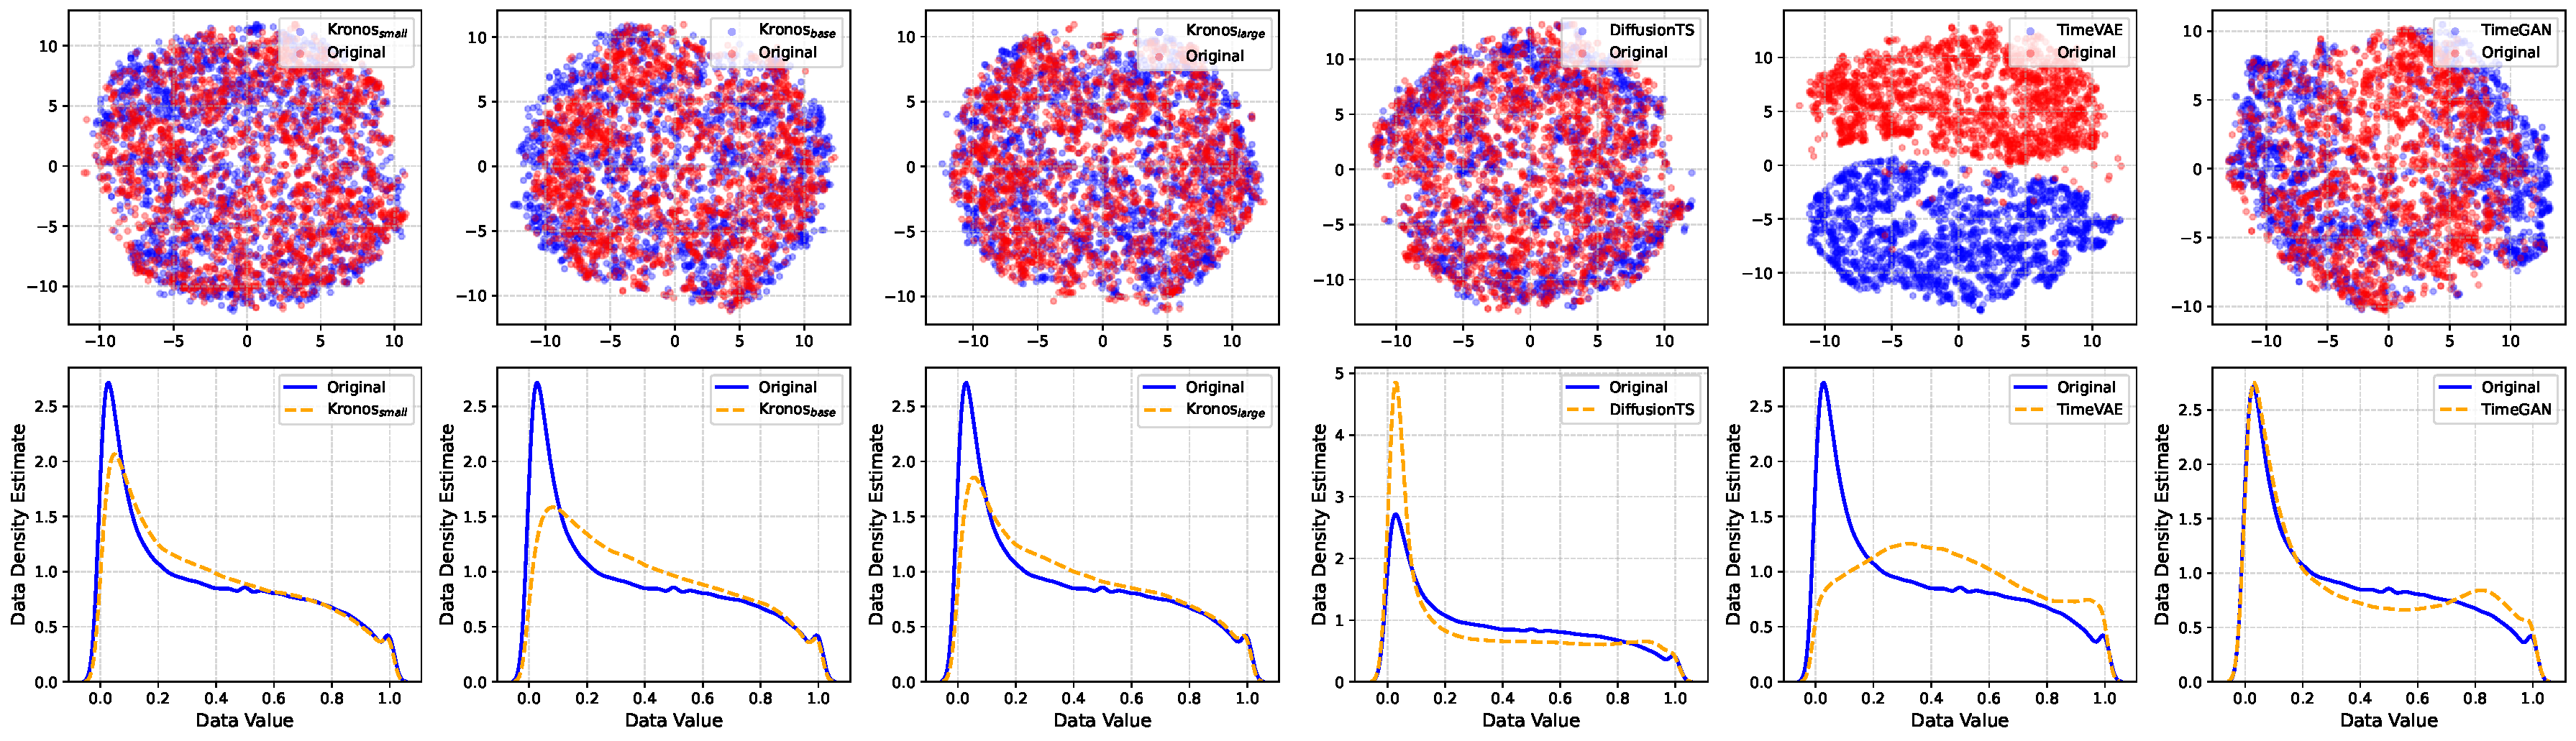
\includegraphics[width=1.0\textwidth]{img/gen_diversity_XTAI_15min.pdf}
        \caption{Taiwan Stock Exchange (XTAI), 15분 빈도}
    \end{subfigure}

    \begin{subfigure}{\textwidth}
        \centering
        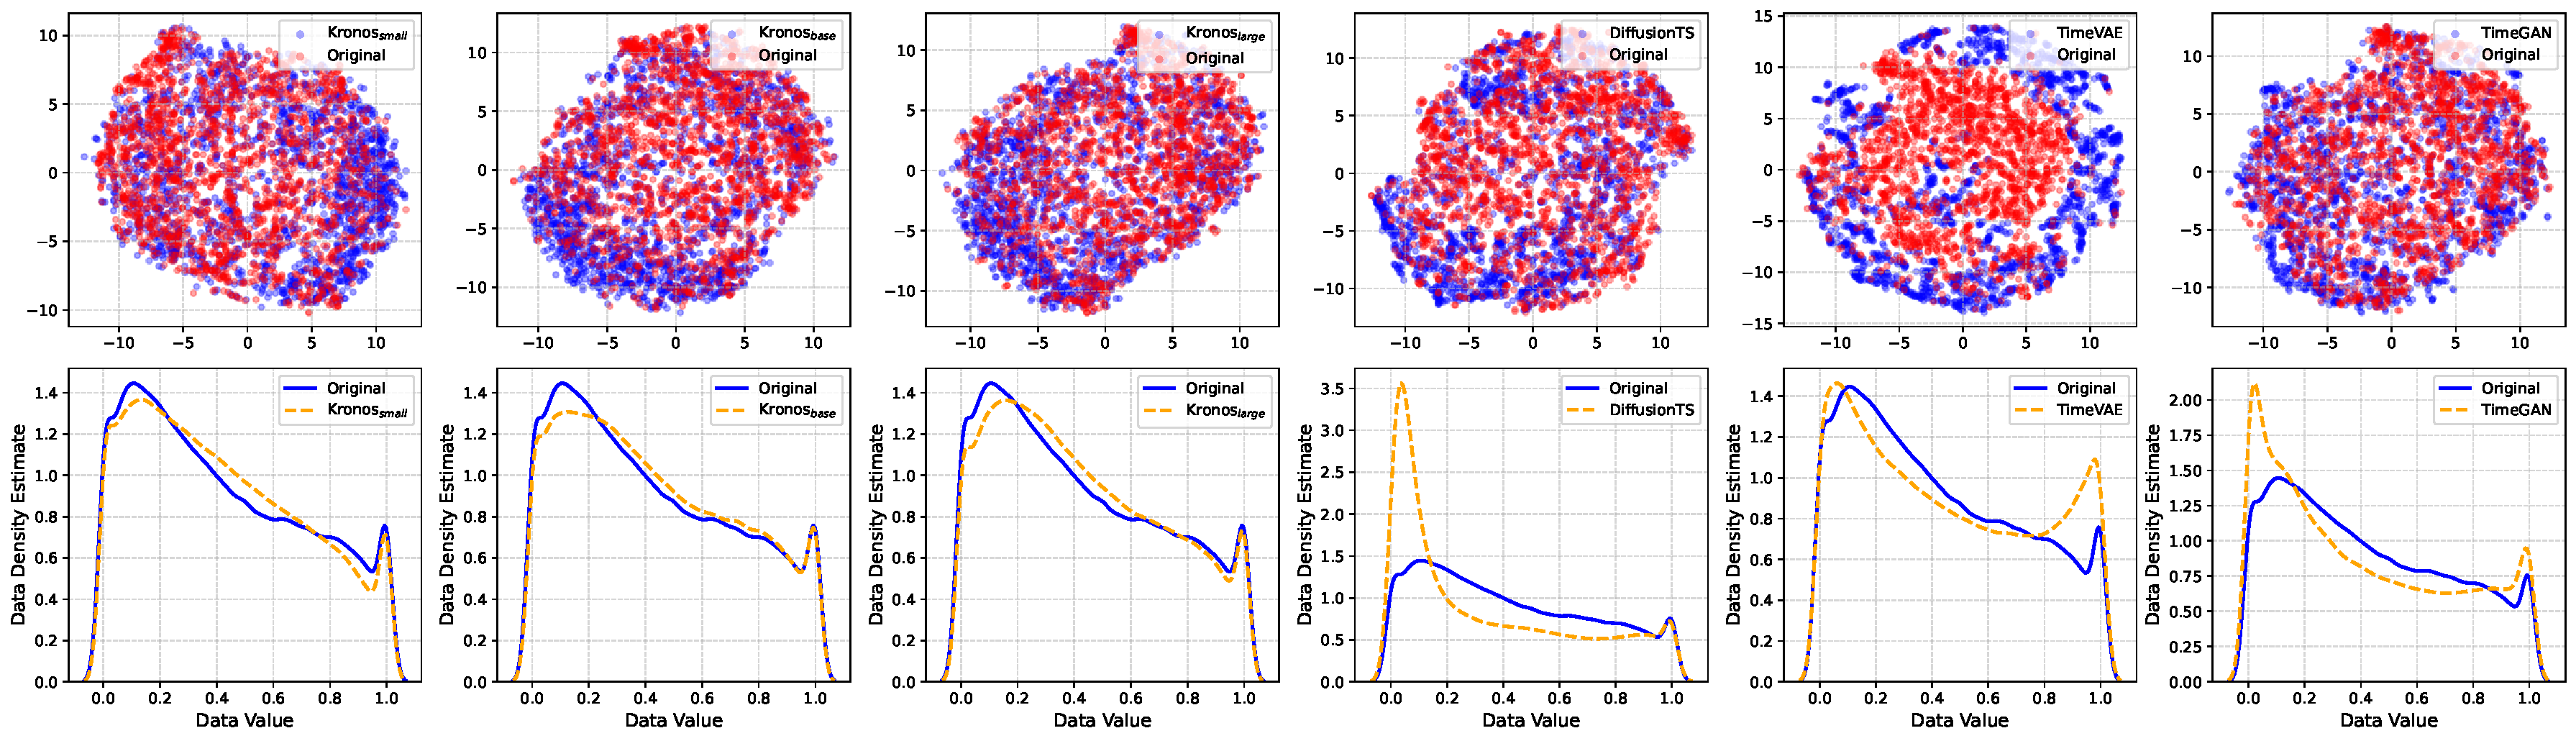
\includegraphics[width=1.0\textwidth]{img/gen_diversity_XTAI_daily.pdf}
        \caption{Taiwan Stock Exchange (XTAI), 일간 빈도}
    \end{subfigure}

    \begin{subfigure}{\textwidth}
        \centering
        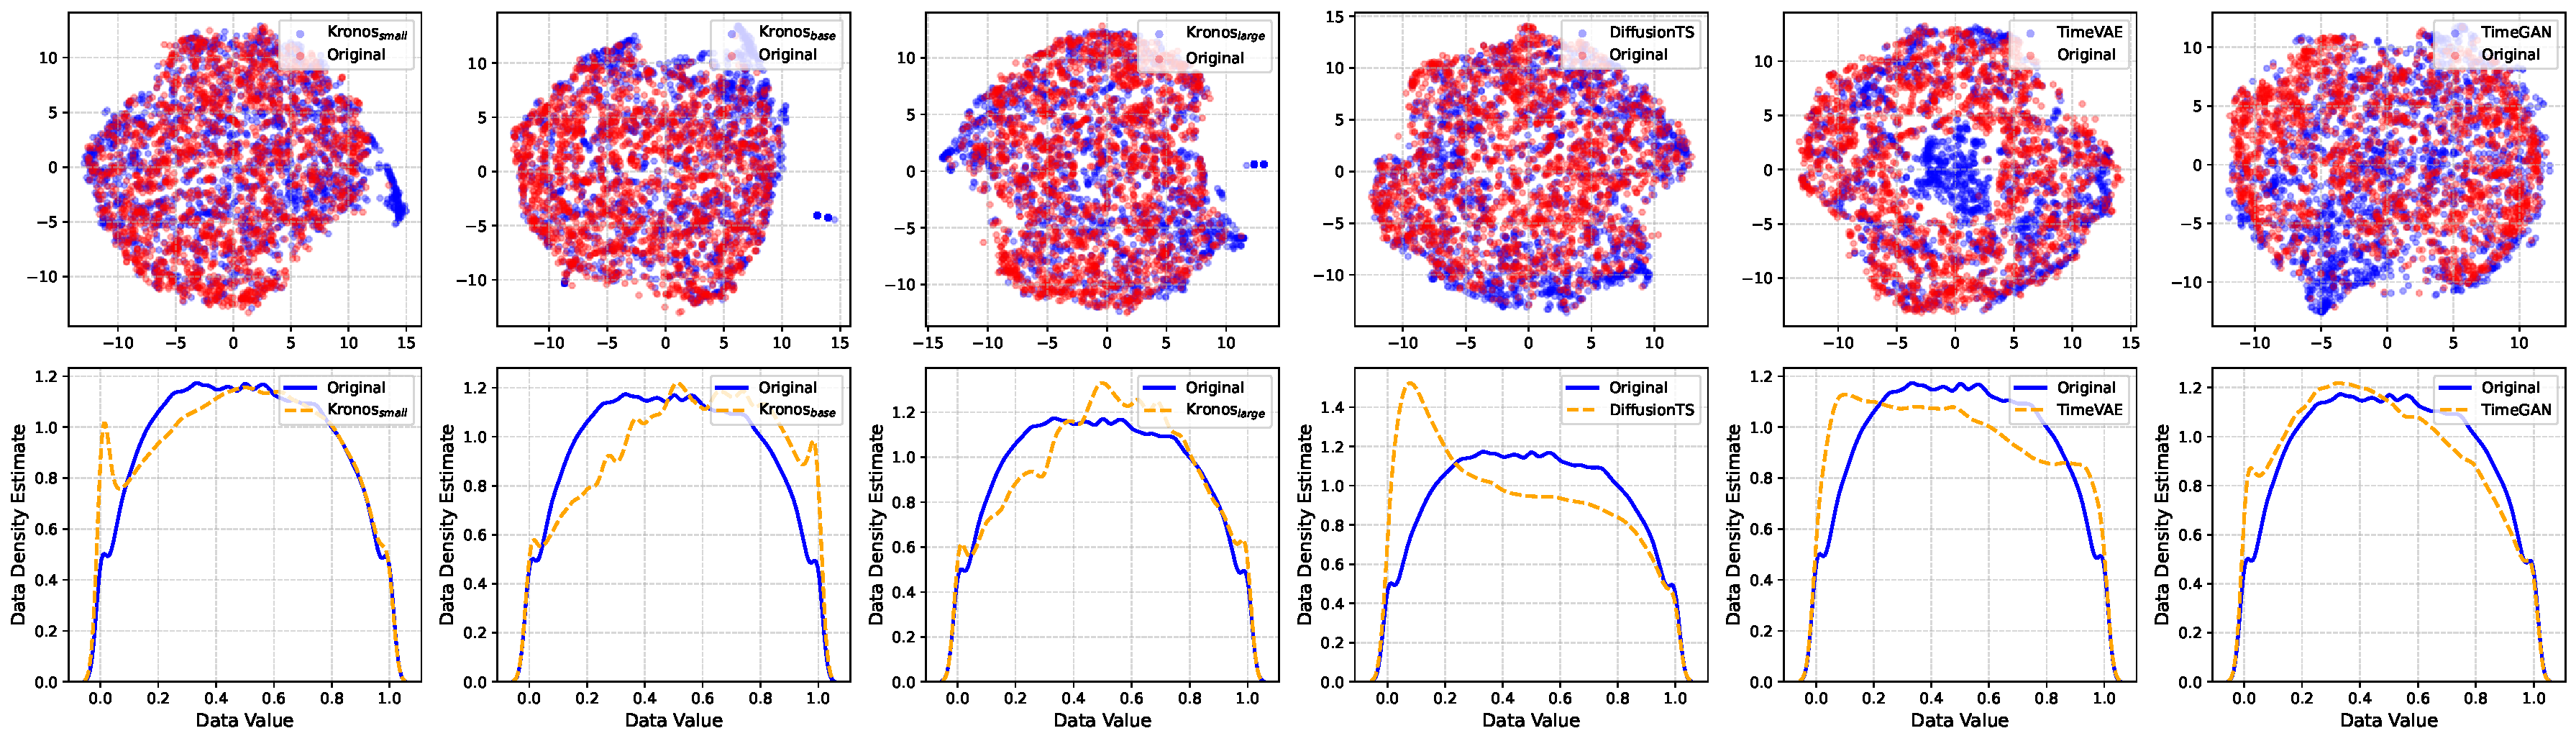
\includegraphics[width=1.0\textwidth]{img/gen_diversity_crypto_15min.pdf}
        \caption{암호화폐 (Crypto), 15분 빈도}
    \end{subfigure}

    \caption{
    서로 다른 데이터셋에서 생성 모델의 시각적 비교.
    \textbf{각 하위 그림의 위 행:} 원본 (\textcolor{red}{red}) 데이터와 합성 (\textcolor{blue}{blue}) 데이터의 t-SNE 임베딩.
    \textbf{각 하위 그림의 아래 행:} 원본 데이터와 합성 데이터의 커널 밀도 추정(KDE).}
    \label{fig:gen_visual_1}
\end{figure*}

\begin{figure*}[htbp]
    \centering

    % \captionsetup{labelformat=empty}

    \begin{subfigure}{\textwidth}
        \centering
        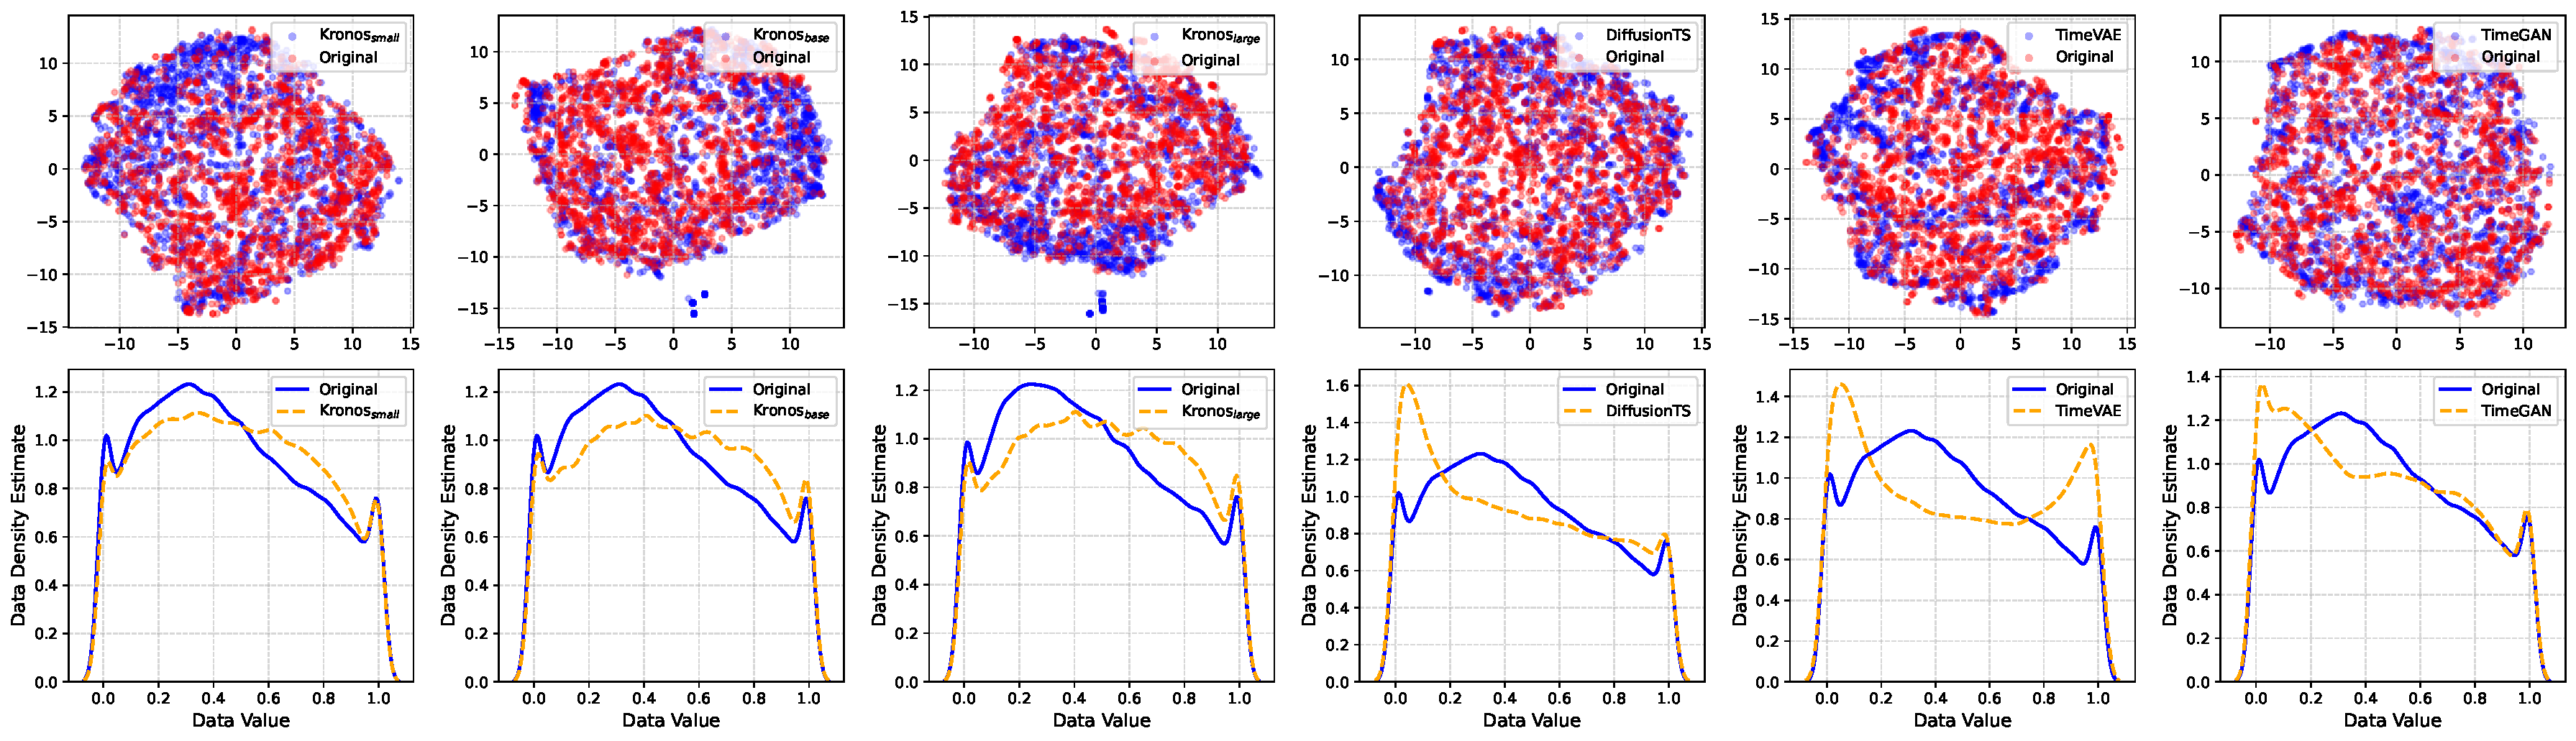
\includegraphics[width=1.0\textwidth]{img/gen_diversity_crypto_daily.pdf}
        \caption{암호화폐 (Crypto), 일간 빈도}
    \end{subfigure}

    \begin{subfigure}{\textwidth}
        \centering
        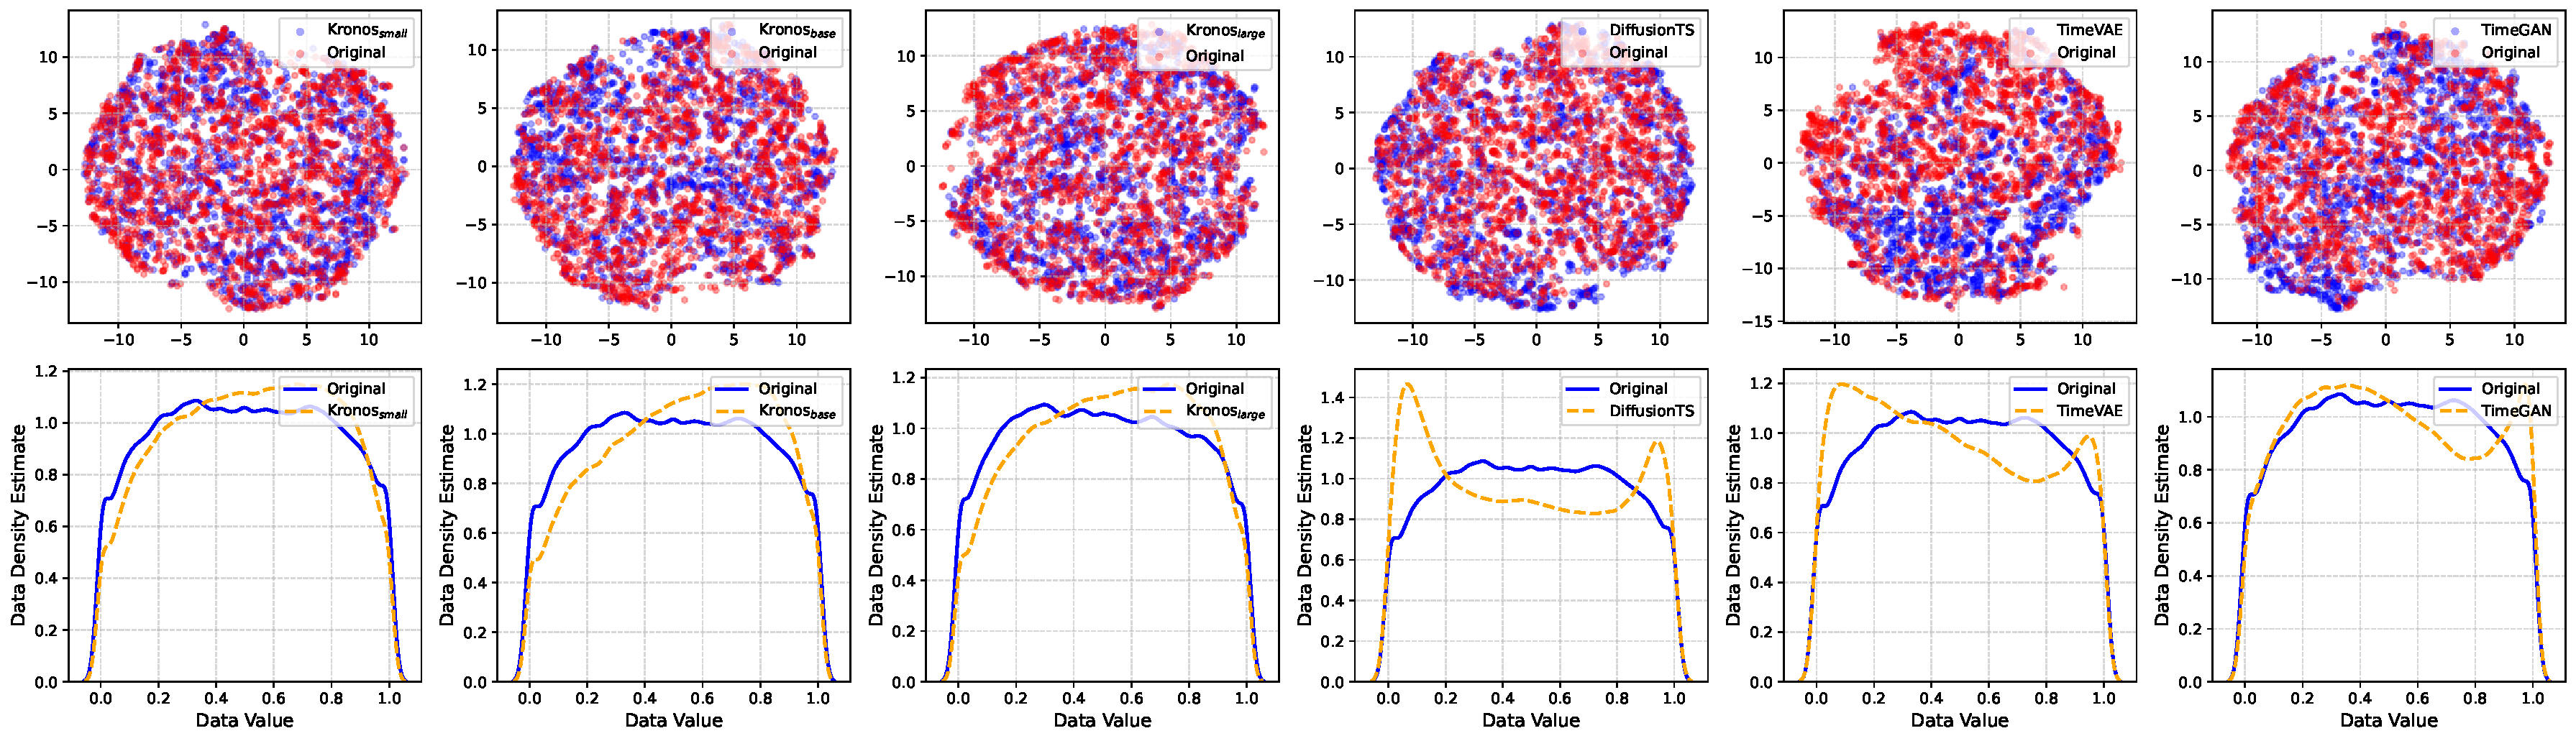
\includegraphics[width=1.0\textwidth]{img/gen_diversity_forex_15min.pdf}
        \caption{외환 (Forex), 15분 빈도}
    \end{subfigure}

    \begin{subfigure}{\textwidth}
        \centering
        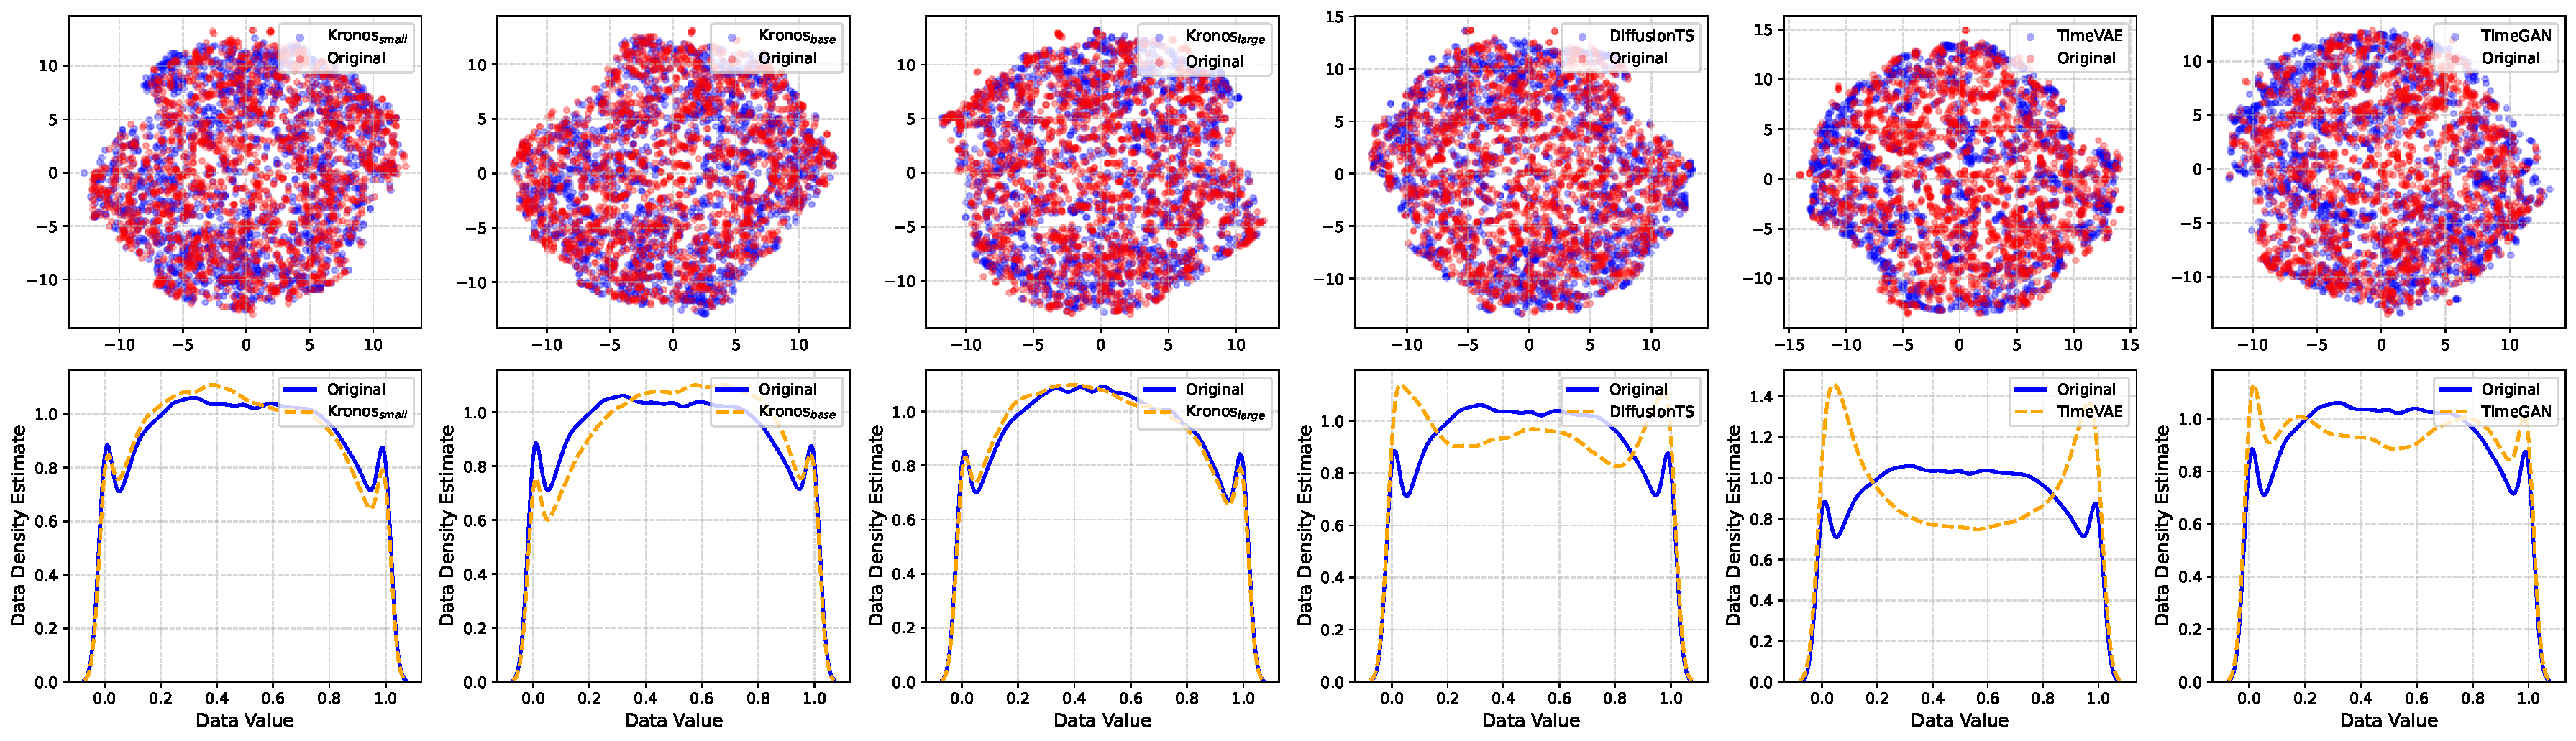
\includegraphics[width=1.0\textwidth]{img/gen_diversity_forex_daily.pdf}
        \caption{외환 (Forex), 일간 빈도}
    \end{subfigure}


    \caption{서로 다른 데이터셋에서 생성 모델의 시각적 비교.
    \textbf{각 하위 그림의 위 행:} 원본 (\textcolor{red}{red}) 데이터와 합성 (\textcolor{blue}{blue}) 데이터의 t-SNE 임베딩.
    \textbf{각 하위 그림의 아래 행:} 원본 데이터와 합성 데이터의 커널 밀도 추정(KDE).}
    \label{fig:gen_visual_2}
\end{figure*}




\begin{table*}[t]
  \centering
  \footnotesize
  \setlength{\tabcolsep}{4pt}

  \adjustbox{max width=\textwidth}{
  \begin{tabular}{l|c|*{11}{S}}
    \toprule
    \multicolumn{2}{c}{\textbf{모델}} &
    \multicolumn{3}{c}{\textbf{
\includegraphics[height=0.25cm]{img/logo_paper.png}\hspace{0.2em}Kronos (Ours)}} &
    \multicolumn{8}{c}{\textbf{Full-shot 시계열 모델}}\\
    \cmidrule(lr){3-5} \cmidrule(lr){6-13}
    \multicolumn{2}{c}{\textbf{지표}} &
    \textbf{$\text{Kronos}_S$} & \textbf{$\text{Kronos}_B$} & \textbf{$\text{Kronos}_L$} &
    \textbf{TimeXer} & \textbf{TimeMixer} & \textbf{iTransformer} & \textbf{PatchTST} &
    \textbf{TimesNet} & \textbf{DLinear} & \textbf{FEDformer} & \textbf{NSTransformer} \\
    \midrule

        \multirow{2}{*}{XSHG} & IC     & \best{0.0549} & \second{0.0564} & 0.0546 & 0.0280 & 0.0291 & 0.0350 & 0.0450 & 0.0424 & 0.0405 & 0.0233 & 0.0433 \\
                              & RankIC & 0.0375 & \best{0.0390} & \second{0.0381} & 0.0053 & 0.0079 & 0.0128 & 0.0088 & 0.0175 & 0.0181 & 0.0107 & 0.0155 \\
        \midrule
        \multirow{2}{*}{XNAS} & IC     & \second{0.0343} & 0.0322 & \best{0.0361} & 0.0132 & 0.0097 & 0.0204 & 0.0116 & 0.0174 & 0.0197 & 0.0165 & 0.0253 \\
                              & RankIC & 0.0155 & \second{0.0190} & \best{0.0191} & 0.0106 & 0.0048 & 0.0111 & 0.0083 & 0.0084 & 0.0084 & -0.0014 & 0.0016 \\
        \midrule
        \multirow{2}{*}{XJPX} & IC     & 0.0314 & \second{0.0332} & \best{0.0360} & 0.0094 & 0.0017 & 0.0137 & 0.0053 & 0.0099 & 0.0118 & 0.0046 & 0.0281 \\
                              & RankIC & 0.0199 & 0.0209 & \best{0.0277} & 0.0159 & 0.0036 & \second{0.0271} & 0.0056 & 0.0127 & 0.0149 & 0.0024 & 0.0212 \\
        \midrule
        \multirow{2}{*}{XNSE} & IC     & \second{0.0634} & \best{0.0648} & \second{0.0634} & -0.0055 & 0.0094 & -0.0252 & 0.0082 & 0.0566 & 0.0024 & 0.0063 & 0.0514 \\
                              & RankIC & 0.0434 & \second{0.0464} & \best{0.0486} & -0.0371 & 0.0024 & -0.0248 & 0.0084 & 0.0379 & -0.0024 & 0.0003 & 0.0225 \\
        \midrule
        \multirow{2}{*}{XKRX} & IC     & 0.0550 & \best{0.0575} & \second{0.0567} & -0.0328 & 0.0036 & -0.0442 & 0.0248 & 0.0416 & 0.0001 & -0.0070 & 0.0416 \\
                              & RankIC & 0.0362 & \best{0.0393} & \second{0.0373} & -0.0160 & 0.0033 & -0.0284 & 0.0214 & 0.0285 & 0.0006 & -0.0049 & 0.0058 \\
        \midrule
        \multirow{2}{*}{XHKG} & IC     & \second{0.0435} & \best{0.0439} & 0.0428 & 0.0318 & 0.0322 & 0.0336 & 0.0401 & 0.0333 & 0.0392 & 0.0296 & 0.0366 \\
                              & RankIC & 0.0226 & \best{0.0236} & \second{0.0228} & -0.0051 & -0.0009 & -0.0021 & -0.0068 & -0.0040 & -0.0009 & -0.0078 & -0.0017 \\
        \midrule
        \multirow{2}{*}{XIDX} & IC     & \second{0.0551} & \second{0.0551} & \best{0.0573} & -0.0139 & 0.0116 & -0.0233 & 0.0194 & 0.0468 & 0.0158 & 0.0169 & 0.0381 \\
                              & RankIC & 0.0214 & \second{0.0216} & \best{0.0223} & 0.0025 & 0.0046 & 0.0011 & 0.0149 & 0.0171 & 0.0037 & 0.0084 & 0.0051 \\
        \midrule
        \multirow{2}{*}{XKLS} & IC     & \second{0.0411} & 0.0408 & \best{0.0466} & -0.0283 & 0.0079 & -0.0281 & -0.0037 & 0.0341 & 0.0306 & -0.0102 & 0.0101 \\
                              & RankIC & \best{0.0215} & 0.0149 & 0.0167 & 0.0051 & 0.0171 & 0.0024 & -0.0078 & -0.0025 & \second{0.0208} & -0.0169 & -0.0103 \\
        \midrule
        \multirow{2}{*}{XTAI} & IC     & 0.0424 & \second{0.0443} & \best{0.0448} & 0.0282 & 0.0197 & 0.0275 & 0.0328 & 0.0312 & 0.0394 & 0.0249 & 0.0334 \\
                              & RankIC & 0.0301 & \second{0.0320} & \best{0.0342} & -0.0042 & 0.0015 & 0.0111 & 0.0147 & 0.0095 & 0.0192 & 0.0059 & 0.0129 \\
        \midrule
        \multirow{2}{*}{Crypto} & IC     & \best{0.0247} & 0.0209 & \second{0.0211}  & 0.0105 & 0.0128 & 0.0155 & 0.0149 & 0.0192 & 0.0137 & 0.0081 & 0.0164 \\
                                & RankIC & 0.0138 & 0.0135 & 0.0129  & 0.0022 & 0.0038 & 0.0134 & \best{0.0192} & \second{0.0146} & 0.0040 & 0.0000 & 0.0096\\
        \midrule
        \multirow{2}{*}{Forex} & IC     & \second{0.0279} & \best{0.0292} & 0.0244 & 0.0124 & 0.0102 & 0.0142 & 0.0158 & 0.0167 & 0.0227 & 0.0153 & 0.0228 \\
                               & RankIC & \best{0.0177} & 0.0141 & 0.0137 & 0.0134 & 0.0128 & 0.0090 & 0.0085 & \second{0.0175} & 0.0168 & 0.0120 & 0.0079 \\
        \midrule

        \rowcolor{AvgGray}
          & IC &
        0.0431 & \second{0.0435} & \best{0.0440} & 0.0048 & 0.0134 & 0.0036 & 0.0195 & 0.0317 & 0.0214 & 0.0117 & 0.0316 \\
        \rowcolor{AvgGray} \multirow{2}{*}[2.5ex]{\textbf{평균}} & RankIC &
        0.0254 & \second{0.0258} & \best{0.0267} & -0.0007 & 0.0055 & 0.0030 & 0.0087 & 0.0143 & 0.0094 & 0.0008 & 0.0082 \\
         \midrule
    \rowcolor{CntGray}
    \multicolumn{2}{c}{\textbf{$\mathbf{1^{st}}$ 횟수}} &
\cnt{4} & \cnt{7} & \cnt{10} & \cnt{0} & \cnt{0} & \cnt{0} &
\cnt{1} & \cnt{0} & \cnt{0} & \cnt{0} & \cnt{0} \\
    \bottomrule
  \end{tabular}}
  \caption{가격 시계열 예측 실험의 전체 결과(Part 1): 우리 모델(Kronos) 및 full-shot 시계열 모델. IC 또는 RankIC가 높을수록 더 나은 예측을 의미한다. 최고 및 차상위 결과는 각각 \best{빨간 밑줄}과 \second{파란 밑줄}로 표시하였다.}
  \label{tab:full_price_forecasting_1}
\end{table*}

\begin{table*}[t]
    \centering
    \footnotesize
    \setlength{\tabcolsep}{4pt}


    \adjustbox{max width=\textwidth}{
    \begin{tabular}{l|c|*{13}{S}}
        \toprule
        \multicolumn{2}{c}{\textbf{모델}} &
        \multicolumn{12}{c}{\textbf{Zero-shot 시계열 모델}} \\
        \cmidrule(lr){3-14}
        \multicolumn{2}{c}{\textbf{지표}} &
        \textbf{$\text{Time\text{-}MOE}_{S}$} & \textbf{$\text{Time\text{-}MOE}_{B}$} &
        \textbf{$\text{Moirai}_{S}$} & \textbf{$\text{Moirai}_{B}$} & \textbf{$\text{Moirai}_{L}$} &
        \textbf{TimesFM} &
        \textbf{$\text{Moment}_{S}$} & \textbf{$\text{Moment}_{B}$} & \textbf{$\text{Moment}_{L}$} &
        \textbf{$\text{Chronos}_{S}$} & \textbf{$\text{Chronos}_{B}$} & \textbf{$\text{Chronos}_{L}$} \\
        \midrule
        \multirow{2}{*}{XSHG} & IC     & 0.0463 & 0.0493 & -0.0007 & -0.0005 & -0.0002 & 0.0174 & 0.0028 & -0.0032 & -0.0009 & 0.0147 & 0.0069 & 0.0195 \\
                              & RankIC & 0.0304 & 0.0317 & 0.0000 & -0.0012 & 0.0003 & 0.0020 & 0.0003 & -0.0037 & -0.0017 & -0.0026 & -0.0108 & 0.0025 \\
        \midrule
        \multirow{2}{*}{XNAS} & IC     & -0.0032 & -0.0045 & -0.0008 & -0.0005 & 0.0000 & 0.0076 & 0.0010 & -0.0023 & -0.0003 & -0.0025 & -0.0005 & 0.0020 \\
                              & RankIC & -0.0033 & -0.0042 & -0.0008 & 0.0013 & 0.0007 & 0.0112 & -0.0015 & -0.0027 & -0.0007 & -0.0001 & 0.0008 & 0.0030 \\
        \midrule
        \multirow{2}{*}{XJPX} & IC     & 0.0268 & 0.0280 & 0.0012 & 0.0004 & 0.0000 & 0.0076 & -0.0010 & -0.0003 & -0.0027 & 0.0117 & 0.0113 & 0.0067 \\
                              & RankIC & 0.0228 & 0.0230 & 0.0025 & 0.0019 & 0.0016 & 0.0073 & -0.0031 & 0.0010 & -0.0006 & 0.0110 & 0.0123 & 0.0070 \\
        \midrule
        \multirow{2}{*}{XNSE} & IC     & 0.0173 & 0.0190 & -0.0005 & -0.0008 & -0.0006 & 0.0025 & 0.0063 & -0.0129 & -0.0039 & -0.0012 & -0.0049 & 0.0014 \\
                              & RankIC & 0.0155 & 0.0169 & -0.0021 & -0.0021 & -0.0029 & 0.0009 & 0.0060 & -0.0104 & -0.0055 & -0.0041 & -0.0066 & -0.0005 \\
        \midrule
        \multirow{2}{*}{XKRX} & IC     & 0.0113 & 0.0141 & -0.0014 & 0.0006 & -0.0011 & -0.0105 & 0.0056 & -0.0083 & -0.0114 & -0.0009 & -0.0018 & 0.0061 \\
                              & RankIC & 0.0088 & 0.0118 & -0.0020 & 0.0006 & -0.0002 & -0.0097 & 0.0041 & -0.0082 & -0.0069 & -0.0006 & -0.0009 & 0.0072 \\
        \midrule
        \multirow{2}{*}{XHKG} & IC     & 0.0174 & 0.0189 & 0.0000 & -0.0001 & -0.0013 & 0.0117 & 0.0013 & -0.0050 & -0.0003 & 0.0159 & 0.0140 & 0.0166 \\
                              & RankIC & 0.0186 & 0.0201 & 0.0003 & 0.0031 & 0.0011 & 0.0058 & -0.0034 & -0.0013 & 0.0009 & 0.0190 & 0.0179 & 0.0192 \\
        \midrule
        \multirow{2}{*}{XIDX} & IC     & -0.0053 & -0.0052 & -0.0009 & -0.0009 & -0.0003 & 0.0026 & 0.0052 & -0.0094 & -0.0007 & 0.0021 & 0.0042 & 0.0080 \\
                              & RankIC & 0.0002 & 0.0000 & 0.0008 & 0.0012 & 0.0007 & 0.0042 & -0.0015 & -0.0029 & 0.0014 & 0.0087 & 0.0122 & 0.0153 \\
        \midrule
        \multirow{2}{*}{XKLS} & IC     & 0.0123 & 0.0125 & -0.0003 & -0.0028 & 0.0005 & 0.0106 & 0.0045 & -0.0093 & -0.0065 & -0.0080 & -0.0076 & -0.0077 \\
                              & RankIC & 0.0112 & 0.0135 & 0.0010 & 0.0027 & 0.0047 & -0.0052 & 0.0000 & 0.0017 & -0.0031 & 0.0113 & 0.0118 & 0.0114 \\
        \midrule
        \multirow{2}{*}{XTAI} & IC     & 0.0296 & 0.0292 & 0.0005 & 0.0001 & -0.0004 & -0.0002 & 0.0025 & -0.0047 & -0.0046 & 0.0028 & -0.0002 & 0.0080 \\
                              & RankIC & 0.0234 & 0.0224 & 0.0011 & 0.0013 & 0.0003 & -0.0028 & 0.0001 & -0.0023 & -0.0009 & 0.0088 & 0.0060 & 0.0125 \\
        \midrule
        \multirow{2}{*}{Crypto} & IC     & 0.0054 & 0.0037 & -0.0008 & -0.0006 & -0.0004 & -0.0009 & -0.0002 & -0.0004 & -0.0030 & -0.0114 & -0.0129 & -0.0096 \\
                                & RankIC & 0.0069 & 0.0050 & 0.0004 & 0.0011 & 0.0000 & 0.0014 & -0.0011 & -0.0061 & -0.0007 & -0.0051 & -0.0061 & -0.0045 \\
        \midrule
        \multirow{2}{*}{Forex} & IC     & 0.0265 & 0.0267 & -0.0011 & -0.0011 & 0.0000 & 0.0092 & -0.0007 & 0.0008 & 0.0024 & 0.0176 & 0.0143 & 0.0155 \\
                               & RankIC & 0.0115 & 0.0114 & -0.0010 & 0.0005 & -0.0003 & 0.0076 & -0.0014 & -0.0010 & 0.0022 & 0.0168 & 0.0147 & 0.0127 \\
        \midrule

        \rowcolor{AvgGray}
         & IC &
        0.0168 & 0.0174 & -0.0004 & -0.0006 & -0.0003 & 0.0052 & 0.0025 & -0.0050 & -0.0029 & 0.0037 & 0.0021 & 0.0060 \\
        \rowcolor{AvgGray} \multirow{2}{*}[2.5ex]{\textbf{평균}} & RankIC &
        0.0133 & 0.0138 & 0.0000 & 0.0009 & 0.0005 & 0.0021 & -0.0001 & -0.0033 & -0.0014 & 0.0057 & 0.0047 & 0.0078 \\
        \midrule
        \rowcolor{CntGray}
        \multicolumn{2}{c}{\textbf{$\mathbf{1^{st}}$ 횟수}} &
\cnt{0} & \cnt{0} & \cnt{0} & \cnt{0} & \cnt{0} & \cnt{0} &
\cnt{0} & \cnt{0} & \cnt{0} & \cnt{0} & \cnt{0} & \cnt{0} \\
        \bottomrule
    \end{tabular}}
\caption{가격 시계열 예측 실험의 전체 결과(Part 2): zero-shot 시계열 모델. IC 또는 RankIC가 높을수록 더 나은 예측을 의미한다. 최고 및 차상위 결과는 각각 \best{빨간 밑줄}과 \second{파란 밑줄}로 표시하였다.}
    \label{tab:full_price_forecasting_2}
\end{table*}

\begin{table*}[t]
  \centering
  \footnotesize
  \setlength{\tabcolsep}{4pt}

  \adjustbox{max width=\textwidth}{
  \begin{tabular}{l|c|*{11}{S}}
    \toprule
    \multicolumn{2}{c}{\textbf{모델}} &
    \multicolumn{3}{c}{\textbf{
\includegraphics[height=0.25cm]{img/logo_paper.png}\hspace{0.2em}Kronos (Ours)}} &
    \multicolumn{8}{c}{\textbf{Full-shot 시계열 모델}}\\
    \cmidrule(lr){3-5} \cmidrule(lr){6-13}
    \multicolumn{2}{c}{\textbf{지표}} &
    \textbf{$\text{Kronos}_S$} & \textbf{$\text{Kronos}_B$} & \textbf{$\text{Kronos}_L$} &
    \textbf{TimeXer} & \textbf{TimeMixer} & \textbf{iTransformer} & \textbf{PatchTST} &
    \textbf{TimesNet} & \textbf{DLinear} & \textbf{FEDformer} & \textbf{NSTransformer}\\
    \midrule

        % ------------------- 데이터 영역 업데이트됨 -------------------
        \multirow{2}{*}{XSHG} & IC     & \second{0.0677} & 0.0652 & 0.0662 & 0.0456 & 0.0114 & 0.0371 & 0.0467 & 0.0563 & 0.0626 & 0.0589 & \best{0.0777} \\
                              & RankIC & 0.0617 & 0.0653 & 0.0642 & 0.0306 & -0.0072 & 0.0266 & 0.0437 & 0.0421 & 0.0461 & 0.0568 & 0.0595 \\
        \midrule
        \multirow{2}{*}{XNAS} & IC     & 0.0563 & \second{0.0626} & \best{0.0639} & 0.0051 & 0.0270 & 0.0340 & 0.0569 & -0.0193 & 0.0144 & 0.0219 & 0.0377 \\
                              & RankIC & 0.0513 & \second{0.0544} & \best{0.0601} & 0.0061 & 0.0204 & 0.0251 & 0.0446 & 0.0352 & 0.0518 & 0.0254 & 0.0335 \\
        \midrule
        \multirow{2}{*}{XJPX} & IC     & 0.0618 & \second{0.0667} & \best{0.0668} & 0.0309 & 0.0211 & 0.0439 & 0.0655 & 0.0656 & 0.0621 & 0.0409 & 0.0436 \\
                              & RankIC & 0.0583 & 0.0623 & 0.0687 & 0.0474 & 0.0145 & 0.0399 & 0.0446 & 0.0556 & 0.0253 & 0.0373 & 0.0428 \\
        \midrule
        \multirow{2}{*}{XNSE} & IC     & 0.0501 & \second{0.0523} & \best{0.0585} & -0.0021 & -0.0126 & 0.0117 & 0.0216 & 0.0238 & 0.0144 & 0.0238 & 0.0314 \\
                              & RankIC & 0.0541 & \second{0.0550} & \best{0.0639} & 0.0031 & 0.0044 & 0.0146 & 0.0238 & 0.0277 & 0.0442 & 0.0130 & 0.0312 \\
        \midrule
        \multirow{2}{*}{XKRX} & IC     & 0.0749 & 0.0778 & \second{0.0792} & 0.0389 & 0.0253 & 0.0309 & 0.0589 & \best{0.0844} & 0.0704 & 0.0726 & 0.0754 \\
                              & RankIC & 0.0707 & 0.0763 & 0.0790 & -0.0024 & -0.0071 & 0.0282 & 0.0422 & \best{0.0801} & 0.0439 & 0.0354 & \second{0.0792} \\
        \midrule
        \multirow{2}{*}{XHKG} & IC     & \best{0.0678} & 0.0661 & 0.0654 & \second{0.0666} & -0.0276 & 0.0106 & 0.0470 & 0.0276 & 0.0404 & 0.0496 & 0.0210 \\
                              & RankIC & 0.0671 & 0.0646 & \second{0.0703} & \best{0.0707} & -0.0063 & 0.0091 & 0.0631 & 0.0288 & 0.0558 & 0.0605 & 0.0264 \\
        \midrule
        \multirow{2}{*}{XIDX} & IC     & \second{0.0998} & 0.0990 & \best{0.1046} & 0.0039 & -0.0095 & 0.0393 & 0.0003 & 0.0301 & 0.0195 & -0.0007 & 0.0244 \\
                              & RankIC & \second{0.0943} & 0.0924 & \best{0.1007} & -0.0111 & -0.0018 & 0.0341 & 0.0280 & 0.0304 & 0.0184 & 0.0358 & 0.0610 \\
        \midrule
        \multirow{2}{*}{XKLS} & IC     & \second{0.1213} & 0.1153 & \best{0.1359} & 0.0144 & 0.0074 & 0.0252 & 0.0605 & 0.0941 & 0.0781 & -0.0016 & 0.1046 \\
                              & RankIC & \second{0.1047} & 0.1009 & \best{0.1145} & -0.0261 & 0.0097 & 0.0237 & 0.0685 & 0.0712 & 0.0800 & -0.0050 & 0.0851 \\
        \midrule
        \multirow{2}{*}{XTAI} & IC     & \best{0.0549} & \second{0.0524} & 0.0511 & 0.0382 & -0.0038 & 0.0313 & 0.0421 & 0.0216 & 0.0514 & 0.0489 & 0.0143 \\
                              & RankIC & \second{0.0597} & 0.0584 & \best{0.0609} & 0.0404 & -0.0027 & 0.0163 & 0.0363 & 0.0261 & 0.0431 & 0.0444 & 0.0159 \\
        \midrule
        \multirow{2}{*}{Crypto} & IC     & 0.0373 & \second{0.0376} & 0.0368  & 0.0286 & 0.0250 & 0.0372 & 0.0163 & 0.0348 & \best{0.0446} & 0.0065 & 0.0274 \\
                                & RankIC & 0.0332 & \best{0.0336} & \second{0.0333}  & 0.0154 & 0.0135 & 0.0151 & 0.0213 & 0.0272 & 0.0283 & 0.0027 & 0.0111\\
        \midrule
        \multirow{2}{*}{Forex} & IC     & 0.0398 & \best{0.0555} & \second{0.0441} & 0.0079 & 0.0203 & 0.0266 & 0.0124 & 0.0054 & 0.0254 & 0.0146 & 0.0122 \\
                               & RankIC & 0.0289 & \best{0.0343} & 0.0274 & 0.0275 & \second{0.0322} & 0.0152 & 0.0148 & 0.0037 & 0.0279 & 0.0148 & 0.0169 \\
        \midrule

        \rowcolor{AvgGray}
          & IC &
        0.0665 & \second{0.0682} & \best{0.0702} & 0.0253 & 0.0076 & 0.0298 & 0.0389 & 0.0386 & 0.0439 & 0.0305 & 0.0427\\
        \rowcolor{AvgGray} \multirow{2}{*}[2.5ex]{\textbf{평균}} & RankIC &
        0.0622 & \second{0.0634} & \best{0.0675} & 0.0183 & 0.0063 & 0.0225 & 0.0392 & 0.0389 & 0.0423 & 0.0292 & 0.0421\\
         \midrule
    \rowcolor{CntGray}
    \multicolumn{2}{c}{\textbf{$\mathbf{1^{st}}$ 횟수}} &
\cnt{2} & \cnt{3} & \cnt{10} & \cnt{1} & \cnt{0} & \cnt{0} &
\cnt{0} & \cnt{2} & \cnt{1} & \cnt{0} & \cnt{1} \\
    \bottomrule
  \end{tabular}}
 \caption{수익률 예측 실험의 전체 결과(Part 1): 우리 모델(Kronos) 및 full-shot 시계열 모델. IC 또는 RankIC가 높을수록 더 나은 예측을 의미한다. 최고 및 차상위 결과는 각각 \best{빨간 밑줄}과 \second{파란 밑줄}로 표시하였다.}
  \label{tab:full_return_forecasting_1}
\end{table*}

\begin{table*}[t]
    \centering
    \footnotesize
    \setlength{\tabcolsep}{4pt}

    \adjustbox{max width=\textwidth}{
    \begin{tabular}{l|c|*{13}{S}}
        \toprule

        \multicolumn{2}{c}{\textbf{모델}} &
        \multicolumn{12}{c}{\textbf{Zero-shot 시계열 모델}} \\
        \cmidrule(lr){3-14}
        \multicolumn{2}{c}{\textbf{지표}} &
        \textbf{$\text{Time\text{-}MOE}_{S}$} & \textbf{$\text{Time\text{-}MOE}_{B}$} &
        \textbf{$\text{Moirai}_{S}$} & \textbf{$\text{Moirai}_{B}$} & \textbf{$\text{Moirai}_{L}$} &
        \textbf{TimesFM} &
        \textbf{$\text{Moment}_{S}$} & \textbf{$\text{Moment}_{B}$} & \textbf{$\text{Moment}_{L}$} &
        \textbf{$\text{Chronos}_{S}$} & \textbf{$\text{Chronos}_{B}$} & \textbf{$\text{Chronos}_{L}$} \\
        \midrule

        \multirow{2}{*}{XSHG} & IC     & 0.0507 & 0.0501 & 0.0507 & 0.0579 & 0.0534 & 0.0322 & 0.0575 & 0.0579 & 0.0575 & -0.0152 & -0.0055 & -0.0019 \\
                              & RankIC & 0.0612 & 0.0621 & \second{0.0657} & 0.0647 & \best{0.0661} & 0.0445 & 0.0527 & 0.0530 & 0.0525 & -0.0277 & -0.0116 & -0.0048 \\
        \midrule
        \multirow{2}{*}{XNAS} & IC     & 0.0416 & 0.0399 & 0.0275 & 0.0281 & 0.0271 & 0.0226 & 0.0290 & 0.0288 & 0.0287 & 0.0545 & 0.0504 & 0.0572 \\
                              & RankIC & 0.0480 & 0.0457 & 0.0280 & 0.0290 & 0.0304 & 0.0271 & 0.0300 & 0.0297 & 0.0296 & 0.0448 & 0.0405 & 0.0461 \\
        \midrule
        \multirow{2}{*}{XJPX} & IC     & 0.0639 & 0.0642 & 0.0441 & 0.0417 & 0.0446 & 0.0498 & 0.0509 & 0.0508 & 0.0512 & 0.0326 & 0.0323 & 0.0276 \\
                              & RankIC & 0.0473 & 0.0487 & \second{0.0790} & \second{0.0790} & \best{0.0793} & 0.0579 & 0.0490 & 0.0491 & 0.0493 & 0.0175 & 0.0174 & 0.0126 \\
        \midrule
        \multirow{2}{*}{XNSE} & IC     & 0.0348 & 0.0343 & 0.0356 & 0.0357 & 0.0354 & 0.0068 & 0.0356 & 0.0357 & 0.0354 & 0.0190 & 0.0179 & 0.0168 \\
                              & RankIC & 0.0476 & 0.0483 & 0.0518 & 0.0518 & 0.0514 & 0.0180 & 0.0518 & 0.0518 & 0.0514 & 0.0116 & 0.0175 & 0.0161 \\
        \midrule
        \multirow{2}{*}{XKRX} & IC     & 0.0573 & 0.0566 & 0.0545 & 0.0546 & 0.0512 & 0.0392 & 0.0545 & 0.0546 & 0.0544 & 0.0523 & 0.0508 & 0.0532 \\
                              & RankIC & 0.0599 & 0.0592 & 0.0617 & 0.0619 & 0.0545 & 0.0465 & 0.0617 & 0.0619 & 0.0618 & 0.0348 & 0.0347 & 0.0394 \\
        \midrule
        \multirow{2}{*}{XHKG} & IC     & 0.0373 & 0.0385 & 0.0324 & 0.0314 & 0.0304 & 0.0281 & 0.0358 & 0.0357 & 0.0357 & 0.0271 & 0.0286 & 0.0297 \\
                              & RankIC & 0.0439 & 0.0431 & 0.0485 & 0.0487 & 0.0486 & 0.0369 & 0.0485 & 0.0487 & 0.0486 & 0.0315 & 0.0331 & 0.0328 \\
        \midrule
        \multirow{2}{*}{XIDX} & IC     & 0.0611 & 0.0565 & 0.0487 & 0.0475 & 0.0474 & 0.0555 & 0.0487 & 0.0488 & 0.0489 & 0.0514 & 0.0560 & 0.0615 \\
                              & RankIC & 0.0638 & 0.0597 & 0.0586 & 0.0586 & 0.0587 & 0.0582 & 0.0586 & 0.0586 & 0.0587 & 0.0404 & 0.0486 & 0.0522 \\
        \midrule
        \multirow{2}{*}{XKLS} & IC     & 0.0971 & 0.0963 & 0.0815 & 0.0782 & 0.0852 & 0.0585 & 0.0856 & 0.0854 & 0.0854 & 0.0804 & 0.0788 & 0.0772 \\
                              & RankIC & 0.0954 & 0.0952 & 0.1004 & 0.1001 & 0.0999 & 0.0710 & 0.0803 & 0.0800 & 0.0799 & 0.0723 & 0.0698 & 0.0697 \\
        \midrule
        \multirow{2}{*}{XTAI} & IC     & 0.0386 & 0.0369 & 0.0418 & 0.0414 & 0.0412 & 0.0332 & 0.0418 & 0.0414 & 0.0412 & 0.0361 & 0.0359 & 0.0338 \\
                              & RankIC & 0.0238 & 0.0202 & 0.0494 & 0.0488 & 0.0487 & 0.0505 & 0.0394 & 0.0388 & 0.0387 & 0.0264 & 0.0326 & 0.0312 \\
        \midrule
        \multirow{2}{*}{Crypto} & IC     & 0.0291 & 0.0293 & -0.0051 & -0.0081 & -0.0046 & -0.0042 & -0.0042 & -0.0039 & -0.0043 & 0.0041 & 0.0067 & 0.0107 \\
                                & RankIC & 0.0122 & 0.0112 & 0.0157 & 0.0172 & 0.0159 & 0.0105 & 0.0058 & 0.0071 & 0.0059 & -0.0069 & -0.0064 & 0.0009 \\
        \midrule
        \multirow{2}{*}{Forex} & IC     & 0.0334 & 0.0336 & 0.0355 & 0.0357 & 0.0347 & 0.0353 & 0.0155 & 0.0157 & 0.0157 & 0.0289 & 0.0255 & 0.0274 \\
                               & RankIC & 0.0217 & 0.0215 & 0.0262 & 0.0264 & 0.0264 & 0.0276 & 0.0162 & 0.0164 & 0.0164 & 0.0194 & 0.0218 & 0.0184 \\
        \midrule

        \rowcolor{AvgGray}
         & IC &
        0.0495 & 0.0487 & 0.0407 & 0.0404 & 0.0405 & 0.0325 & 0.0410 & 0.0410 & 0.0409 & 0.0337 & 0.0343 & 0.0357 \\
        \rowcolor{AvgGray} \multirow{2}{*}[2.5ex]{\textbf{평균}} & RankIC &
        0.0477 & 0.0468 & 0.0532 & 0.0533 & 0.0527 & 0.0408 & 0.0449 & 0.0450 & 0.0448 & 0.0240 & 0.0271 & 0.0286 \\
        \midrule
        \rowcolor{CntGray}
        \multicolumn{2}{c}{\textbf{$\mathbf{1^{st}}$ 횟수}} &
\cnt{0} & \cnt{0} & \cnt{0} & \cnt{0} & \cnt{2} & \cnt{0} &
\cnt{0} & \cnt{0} & \cnt{0} & \cnt{0} & \cnt{0} & \cnt{0} \\
        \bottomrule
    \end{tabular}}
\caption{수익률 예측 실험의 전체 결과(Part 2): zero-shot 시계열 모델. IC 또는 RankIC가 높을수록 더 나은 예측을 의미한다. 최고 및 차상위 결과는 각각 \best{빨간 밑줄}과 \second{파란 밑줄}로 표시하였다.}
    \label{tab:full_return_forecasting_2}
\end{table*}

\begin{table*}[t]
  \centering
  \footnotesize
  \setlength{\tabcolsep}{4pt}

  \adjustbox{max width=\textwidth}{
  \begin{tabular}{l|c|*{13}{S}}
    \toprule
    \multicolumn{2}{c}{\textbf{모델}} &
    \multicolumn{3}{c}{\textbf{
\includegraphics[height=0.25cm]{img/logo_paper.png}\hspace{0.2em}Kronos (Ours)}} &
    \multicolumn{8}{c}{\textbf{Full-shot 시계열 모델}} & \multicolumn{2}{c}{\textbf{계량경제 변동성 모델}}\\
    \cmidrule(lr){3-5} \cmidrule(lr){6-13} \cmidrule(lr){14-15}
    \multicolumn{2}{c}{\textbf{지표}} &
    \textbf{$\text{Kronos}_S$} & \textbf{$\text{Kronos}_B$} & \textbf{$\text{Kronos}_L$} &
    \textbf{TimeXer} & \textbf{TimeMixer} & \textbf{iTransformer} & \textbf{PatchTST} &
    \textbf{TimesNet} & \textbf{DLinear} & \textbf{FEDformer} & \textbf{NSTransformer} & \textbf{ARCH} & \textbf{GARCH} \\
    \midrule

        \multirow{2}{*}{XSHG} & MAE     & \best{0.0199} & 0.0205 & \second{0.0203} & 0.0510 & 0.0349 & 0.0593 & 0.0356 & 0.0348 & 0.0398 & 0.0231 & 0.0348 & 0.0247 & 0.0219 \\
                              & $R^2$ & 0.2597 & \second{0.2630} & \best{0.2809} & 0.1500 & 0.1585 & 0.2191 & 0.2401 & 0.1429 & 0.2400 & 0.2301 & 0.1232 & 0.1969 & 0.1986 \\
        \midrule
        \multirow{2}{*}{XNAS} & MAE     & 0.1540 & 0.1407 & 0.1503 & 0.3323 & 0.3473 & 0.3223 & 0.2926 & 0.2492 & 0.2416 & 0.2223 & 0.2168 & 0.1472 & 0.1259 \\
                              & $R^2$ & 0.1169 & 0.0961 & 0.0978 & 0.0819 & 0.0071 & 0.0876 & 0.1036 & 0.0452 & 0.1192 & 0.0512 & 0.0963 & \second{0.2174} & \best{0.2271} \\
        \midrule
        \multirow{2}{*}{XJPX} & MAE     & \second{0.0198} & \second{0.0198} & \best{0.0196} & 0.1309 & 0.1324 & 0.0425 & 0.0842 & 0.0365 & 0.1527 & 0.0316 & 0.0353 & 0.0320 & 0.0271 \\
                              & $R^2$ & 0.1626 & 0.1912 & 0.1996 & 0.1818 & 0.0229 & 0.1245 & 0.0383 & 0.1277 & 0.0133 & 0.0467 & 0.1531 & \second{0.2421} & \best{0.2434} \\
        \midrule
        \multirow{2}{*}{XNSE} & MAE     & \best{0.0264} & 0.0269 & \second{0.0267} & 0.0667 & 0.0347 & 0.0502 & 0.0784 & 0.0555 & 0.1272 & 0.0614 & 0.0497 & 0.0269 & 0.0271 \\
                              & $R^2$ & \second{0.1803} & 0.1445 & \best{0.1815} & 0.1184 & 0.0708 & 0.1140 & 0.0153 & 0.0486 & 0.0152 & 0.0286 & 0.0365 & 0.1424 & 0.1548 \\
        \midrule
        \multirow{2}{*}{XKRX} & MAE     & 0.0271 & \second{0.0255} & \best{0.0246} & 0.0332 & 0.0424 & 0.0408 & 0.0449 & 0.0537 & 0.0608 & 0.0715 & 0.0552 & 0.0347 & 0.0316 \\
                              & $R^2$ & 0.5936 & \best{0.6190} & \second{0.6156} & 0.1966 & 0.0175 & 0.1967 & 0.1792 & 0.2695 & 0.0795 & 0.0842 & 0.2223 & 0.4617 & 0.4641 \\
        \midrule
        \multirow{2}{*}{XHKG} & MAE     & \second{0.0352} & 0.0402 & \best{0.0349} & 0.0435 & 0.0746 & 0.0679 & 0.0547 & 0.0608 & 0.0529 & 0.0702 & 0.0499 & 0.0464 & 0.0402 \\
                              & $R^2$ & 0.1935 & 0.1875 & 0.1824 & 0.1423 & 0.0515 & 0.0394 & 0.0408 & 0.0396 & 0.0482 & 0.0176 & 0.0051 & \second{0.3294} & \best{0.3295} \\
        \midrule
        \multirow{2}{*}{XIDX} & MAE     & 0.0566 & \second{0.0544} & \best{0.0501} & 0.1412 & 0.2504 & 0.0925 & 0.0728 & 0.0827 & 0.1263 & 0.0987 & 0.0836 & 0.0647 & 0.0592 \\
                              & $R^2$ & 0.1275 & 0.1884 & 0.1467 & 0.1443 & 0.0163 & 0.1730 & 0.0433 & 0.1053 & 0.0322 & 0.0391 & 0.1065 & \best{0.2209} & \second{0.2092} \\
        \midrule
        \multirow{2}{*}{XKLS} & MAE     & \second{0.0370} & \best{0.0367} & 0.0376 & 0.1570 & 0.0823 & 0.0456 & 0.1355 & 0.0759 & 0.0533 & 0.0787 & 0.0827 & 0.0397 & 0.0406 \\
                              & $R^2$ & \best{0.5369} & 0.4781 & \second{0.4967} & 0.1867 & 0.1378 & 0.2245 & 0.1201 & 0.1409 & 0.0529 & 0.0540 & 0.1172 & 0.2148 & 0.2247 \\
        \midrule
        \multirow{2}{*}{XTAI} & MAE     & \second{0.0217} & 0.0220 & \best{0.0213} & 0.0230 & 0.0254 & 0.0267 & 0.0229 & 0.0318 & 0.0262 & 0.0223 & 0.0271 & 0.0263 & 0.0240 \\
                              & $R^2$ & \second{0.2607} & 0.2074 & \best{0.2915} & 0.1755 & 0.1797 & 0.1740 & 0.2171 & 0.1591 & 0.2592 & 0.1853 & 0.1783 & 0.2021 & 0.2320 \\
        \midrule
        \multirow{2}{*}{Crypto} & MAE     & \second{0.0147} & 0.0148 & \best{0.0145}  & 0.1438 & 0.0705 & 0.0346 & 0.0926 & 0.0289 & 0.0446 & 0.0642 & 0.0375 & 0.0286 & 0.0292 \\
                                & $R^2$ & 0.1772 & 0.2179 & \best{0.2658}  & 0.0468 & 0.0711 & 0.1212 & 0.1475 & \second{0.2372} & 0.0547 & 0.0286 & 0.1095 & 0.1642 & 0.1575\\
        \midrule
        \multirow{2}{*}{Forex} & MAE     & 0.0097 & \second{0.0074} & \best{0.0069} & 0.0277 & 0.0277 & 0.0205 & 0.0300 & 0.0187 & 0.0212 & 0.0171 & 0.0176 & 0.0219 & 0.0185 \\
                               & $R^2$ & \best{0.1301} & 0.1235 & \second{0.1277} & 0.0002 & 0.0302 & 0.0290 & 0.0270 & 0.0029 & 0.0901 & 0.0382 & 0.0034 & 0.1169 & 0.1141 \\
        \midrule

        \rowcolor{AvgGray}
          & MAE &
        0.0384 & \second{0.0372} & \best{0.0370} & 0.1046 & 0.1021 & 0.0730 & 0.0858 & 0.0662 & 0.0861 & 0.0692 & 0.0627 & 0.0448 & 0.0405 \\
        \rowcolor{AvgGray} \multirow{2}{*}[2.5ex]{\textbf{평균}} & $R^2$ &
        \second{0.2490} & 0.2470 & \best{0.2624} & 0.1295 & 0.0694 & 0.1366 & 0.1066 & 0.1199 & 0.0913 & 0.0731 & 0.1047 & 0.2281 & 0.2323 \\
         \midrule
    \rowcolor{CntGray}
    \multicolumn{2}{c}{\textbf{$\mathbf{1^{st}}$ 횟수}} &
\cnt{4} & \cnt{2} & \cnt{11} & \cnt{0} & \cnt{0} & \cnt{0} &
\cnt{0} & \cnt{0} & \cnt{0} & \cnt{0} & \cnt{0} & \cnt{1} & \cnt{3} \\
    \bottomrule
  \end{tabular}}
  \caption{실현 변동성 예측 실험의 전체 결과(Part 1): 우리 모델(Kronos) 및 full-shot 시계열 모델. MAE가 낮거나 $R^2$가 높을수록 더 나은 예측을 의미한다. 최고 및 차상위 결과는 각각 \best{빨간 밑줄}과 \second{파란 밑줄}로 표시하였다.}
  \label{tab:full_volatility_forecasting_1}
\end{table*}

\begin{table*}[t]
    \centering
    \footnotesize
    \setlength{\tabcolsep}{4pt}

    \adjustbox{max width=\textwidth}{
    \begin{tabular}{l|c|*{13}{S}}
        \toprule
        \multicolumn{2}{c}{\textbf{모델}} &
        \multicolumn{12}{c}{\textbf{Zero-shot 시계열 모델}} \\
        \cmidrule(lr){3-14}
        \multicolumn{2}{c}{\textbf{지표}} &
        \textbf{$\text{Time\text{-}MOE}_{S}$} & \textbf{$\text{Time\text{-}MOE}_{B}$} &
        \textbf{$\text{Moirai}_{S}$} & \textbf{$\text{Moirai}_{B}$} & \textbf{$\text{Moirai}_{L}$} &
        \textbf{TimesFM} &
        \textbf{$\text{Moment}_{S}$} & \textbf{$\text{Moment}_{B}$} & \textbf{$\text{Moment}_{L}$} &
        \textbf{$\text{Chronos}_{S}$} & \textbf{$\text{Chronos}_{B}$} & \textbf{$\text{Chronos}_{L}$} \\
        \midrule
        % ------------------- 데이터 영역 -------------------
        \multirow{2}{*}{XSHG} & MAE     & 0.0462 & 0.0471 & 0.1158 & 0.0994 & 0.1048 & 0.0408 & 0.0357 & 0.0343 & 0.0366 & 0.0386 & 0.0384 & 0.0382 \\
                              & $R^2$ & 0.2423 & 0.2417 & 0.2118 & 0.2233 & 0.2191 & 0.0995 & 0.2479 & 0.2461 & 0.2336 & 0.1946 & 0.1922 & 0.1663 \\
        \midrule
        \multirow{2}{*}{XNAS} & MAE     & 0.2713 & 0.2498 & 0.3537 & 0.1927 & 0.2502 & 0.1902 & \second{0.1034} & \best{0.1020} & 0.1168 & 0.1896 & 0.1863 & 0.1881 \\
                              & $R^2$ & 0.1255 & 0.0901 & 0.1782 & 0.1228 & 0.1306 & 0.0740 & 0.0872 & 0.0882 & 0.0804 & 0.0811 & 0.0340 & 0.0982 \\
        \midrule
        \multirow{2}{*}{XJPX} & MAE     & 0.0372 & 0.0367 & 0.1065 & 0.0829 & 0.0878 & 0.0345 & 0.0291 & 0.0278 & 0.0306 & 0.0331 & 0.0331 & 0.0329 \\
                              & $R^2$ & 0.1392 & 0.1374 & 0.1150 & 0.1541 & 0.1493 & 0.1213 & 0.1489 & 0.1450 & 0.01375 & 0.1812 & 0.1794 & 0.1769 \\
        \midrule
        \multirow{2}{*}{XNSE} & MAE     & 0.0420 & 0.0415 & 0.1029 & 0.0873 & 0.0924 & 0.0437 & 0.0364 & 0.0358 & 0.0397 & 0.0414 & 0.0413 & 0.0411 \\
                              & $R^2$ & 0.0411 & 0.0457 & 0.0455 & 0.0588 & 0.0554 & 0.0394 & 0.0483 & 0.0468 & 0.0422 & 0.0454 & 0.0563 & 0.0439 \\
        \midrule
        \multirow{2}{*}{XKRX} & MAE     & 0.0452 & 0.0447 & 0.1109 & 0.0909 & 0.0982 & 0.0508 & 0.0418 & 0.0413 & 0.0461 & 0.0485 & 0.0484 & 0.0482 \\
                              & $R^2$ & 0.2248 & 0.2321 & 0.2235 & 0.2576 & 0.2229 & 0.1249 & 0.2914 & 0.2811 & 0.2588 & 0.3357 & 0.3371 & 0.3132 \\
        \midrule
        \multirow{2}{*}{XHKG} & MAE     & 0.0701 & 0.0671 & 0.1824 & 0.1367 & 0.1499 & 0.0551 & 0.0500 & 0.0475 & 0.0499 & 0.0526 & 0.0523 & 0.0521 \\
                              & $R^2$ & 0.1757 & 0.1475 & 0.0900 & 0.1838 & 0.1576 & 0.1862 & 0.1537 & 0.1502 & 0.1432 & 0.1064 & 0.1018 & 0.1090 \\
        \midrule
        \multirow{2}{*}{XIDX} & MAE     & 0.0725 & 0.0718 & 0.2321 & 0.1687 & 0.1876 & 0.0766 & 0.0652 & 0.0695 & 0.0663 & 0.0744 & 0.0735 & 0.0732 \\
                              & $R^2$ & 0.1558 & 0.1572 & 0.1228 & 0.1118 & 0.1144 & 0.0952 & 0.1607 & 0.1093 & 0.1471 & 0.1445 & 0.1820 & 0.1692 \\
        \midrule
        \multirow{2}{*}{XKLS} & MAE     & 0.0572 & 0.0553 & 0.1142 & 0.0914 & 0.1037 & 0.0733 & 0.0571 & 0.0597 & 0.0699 & 0.0706 & 0.0705 & 0.0703 \\
                              & $R^2$ & 0.0828 & 0.1021 & 0.1451 & 0.1559 & 0.1669 & 0.0541 & 0.1714 & 0.1725 & 0.1393 & 0.1673 & 0.1745 & 0.1645 \\
        \midrule
        \multirow{2}{*}{XTAI} & MAE     & 0.0387 & 0.0384 & 0.1047 & 0.0900 & 0.0954 & 0.0386 & 0.0335 & 0.0319 & 0.0341 & 0.0371 & 0.0369 & 0.0366 \\
                              & $R^2$ & 0.1901 & 0.1913 & 0.1611 & 0.1704 & 0.1729 & 0.0789 & 0.1885 & 0.1850 & 0.1672 & 0.1868 & 0.1804 & 0.1588 \\
        \midrule
        \multirow{2}{*}{Crypto} & MAE     & 0.0374 & 0.0373 & 0.0570 & 0.0574 & 0.0572 & 0.0352 & 0.0209 & 0.0236 & 0.0327 & 0.0341 & 0.0340 & 0.0339 \\
                                & $R^2$ & 0.1416 & 0.1387 & 0.1061 & 0.1004 & 0.2016 & 0.0881 & 0.1685 & 0.1310 & 0.1758 & 0.1566 & 0.1608 & 0.1584 \\
        \midrule
        \multirow{2}{*}{Forex} & MAE     & 0.0225 & 0.0110 & 0.0119 & 0.0151 & 0.0120 & 0.0171 & 0.0151 & 0.0155 & 0.0158 & 0.0102 & 0.0124 & 0.0218 \\
                               & $R^2$ & 0.1173 & 0.0286 & 0.0145 & 0.0306 & 0.0504 & 0.0141 & 0.0744 & 0.0592 & 0.0717 & 0.0391 & 0.0245 & 0.0453 \\
        \midrule

        \rowcolor{AvgGray}
         & MAE &
        0.0673 & 0.0637 & 0.1356 & 0.1011 & 0.1127 & 0.0596 & 0.0444 & 0.0444 & 0.0490 & 0.0573 & 0.0570 & 0.0579 \\
        \rowcolor{AvgGray} \multirow{2}{*}[2.5ex]{\textbf{평균}} & $R^2$ &
        0.1487 & 0.1375 & 0.1285 & 0.1427 & 0.1492 & 0.0887 & 0.1380 & 0.1468 & 0.1339 & 0.1490 & 0.1475 & 0.1458 \\
        \midrule
        \rowcolor{CntGray}
        \multicolumn{2}{c}{\textbf{$\mathbf{1^{st}}$ 횟수}} &
\cnt{0} & \cnt{0} & \cnt{0} & \cnt{0} & \cnt{0} & \cnt{0} &
\cnt{0} & \cnt{1} & \cnt{0} & \cnt{0} & \cnt{0} & \cnt{0} \\
        \bottomrule
    \end{tabular}}
    \caption{실현 변동성 예측 실험의 전체 결과(Part 2): zero-shot 시계열 모델. MAE가 낮거나 $R^2$가 높을수록 더 나은 예측을 의미한다. 최고 및 차상위 결과는 각각 \best{빨간 밑줄}과 \second{파란 밑줄}로 표시하였다.}
    \label{tab:full_volatility_forecasting_2}
\end{table*}

\begin{table*}[t]
  \centering
  \footnotesize
  \setlength{\tabcolsep}{4pt}


  \adjustbox{max width=\textwidth}{
  \begin{tabular}{l|c|*{6}{c}}
    \toprule
    \multicolumn{2}{c|}{\textbf{모델}} &
    \multicolumn{3}{c}{\textbf{
\includegraphics[height=0.23cm]{img/logo_paper.png}\hspace{0.2em}Kronos (Ours)}} &
    \multicolumn{3}{c}{\textbf{시계열 생성 모델}} \\
    \cmidrule(lr){3-5} \cmidrule(lr){6-8}
    \multicolumn{2}{c|}{\textbf{지표}} &
    \textbf{$\text{Kronos}_{small}$} & \textbf{$\text{Kronos}_{base}$} & \textbf{$\text{Kronos}_{large}$} &
    \textbf{DiffusionTS} & \textbf{TimeVAE} & \textbf{TimeGAN} \\
    \midrule

    % -------------------- XSHG --------------------
    \multirow{2}{*}{XSHG} & 15분 & \second{0.2313} & 0.2317 & \best{0.2393} & 0.0885 & 0.0015 & 0.2241 \\
                          & 일간 & 0.1865 & \second{0.2227} & 0.2105 & \best{0.2532} & 0.0142 & 0.1193 \\
    \midrule
    % -------------------- XTAI --------------------
    \multirow{2}{*}{XTAI} & 15분 & 0.1733 & 0.1478 & \second{0.1788} & 0.1420 & 0.0387 & \best{0.2689} \\
                          & 일간 & \second{0.2088} & 0.2023 & \best{0.2235} & 0.1712 & 0.0097 & 0.0622 \\
    \midrule
    % -------------------- Crypto ------------------
    \multirow{2}{*}{Crypto} & 15분 & 0.4100 & \second{0.4185} & \best{0.4187} & 0.3005 & 0.0637 & 0.0680 \\
                            & 일간 & 0.2792 & 0.2575 & \second{0.2835} & \best{0.3188} & 0.0402 & 0.2114 \\
    \midrule
    % -------------------- Forex -------------------
    \multirow{2}{*}{Forex} & 15분 & \second{0.4783} & 0.\best{4903} & 0.4688 & 0.4112 & 0.0492 & 0.4015 \\
                           & 일간 & 0.3337 & \best{0.4363} & \second{0.4152} & 0.3177 & 0.0295 & 0.2387 \\
    \midrule

    % -------------------- 평균 -----------------
    \rowcolor{AvgGray}
    \multicolumn{2}{c|}{\textbf{평균}} &
      0.2876 & \second{0.3009} & \best{0.3048} & 0.2504 & 0.0308 & 0.1993 \\
    \midrule

    % -------------------- 1위 횟수 ---------------
    \rowcolor{CntGray}
    \multicolumn{2}{c|}{\textbf{$\mathbf{1^{st}}$ 횟수}} &
      \cnt{0} & \cnt{2} & \cnt{4} & \cnt{2} & \cnt{0} & \cnt{1} \\
    \bottomrule
  \end{tabular}}
  \caption{합성 K-line 생성 실험의 판별 점수 전체 결과. 점수가 높을수록 생성 품질이 더 좋음을 의미한다. 최고 및 차상위 결과는 각각 \best{빨간 밑줄}과 \second{파란 밑줄}로 표시하였다.}
  \label{tab:generate_discriminative}
\end{table*}

\begin{table*}[t]
  \centering
  \footnotesize
  \setlength{\tabcolsep}{4pt}

  \adjustbox{max width=\textwidth}{
  \begin{tabular}{l|c|c|*{6}{S}}
    \toprule
    \multicolumn{3}{c|}{\textbf{모델}} &
    \multicolumn{3}{c}{\textbf{
\includegraphics[height=0.23cm]{img/logo_paper.png}\hspace{0.2em}Kronos (Ours)}} &
    \multicolumn{3}{c}{\textbf{시계열 생성 모델}} \\
    \cmidrule(lr){4-6} \cmidrule(lr){7-9}
    \multicolumn{3}{c|}{\textbf{지표}} &
    \textbf{$\text{Kronos}_{small}$} & \textbf{$\text{Kronos}_{base}$} & \textbf{$\text{Kronos}_{large}$} &
    \textbf{DiffusionTS} & \textbf{TimeVAE} & \textbf{TimeGAN} \\
    \midrule

    % -------------------- 데이터 영역 --------------------
    % ------- XSHG -------
    \multirow{4}{*}{XSHG} & \multirow{2}{*}{15분} & IC      & 0.0223 & \second{0.0231} & \best{0.0236} & 0.0103 & 0.0098 & 0.0102 \\
                          &                        & RankIC  & 0.0144 & \second{0.0147} & \best{0.0151} & 0.0087 & 0.0134 & 0.0081 \\
                          \cmidrule(lr){2-9}
                          & \multirow{2}{*}{일간} & IC      & \best{0.0918} & \second{0.0902} & 0.0845 & 0.0760 & -0.0789 & 0.0108 \\
                          &                        & RankIC  & \best{0.0854} & \second{0.0839} & 0.0796 & 0.0684 & -0.0720 & 0.0150 \\
    \midrule
    % ------- XTAI -------
    \multirow{4}{*}{XTAI} & \multirow{2}{*}{15분} & IC      & 0.0230 & \second{0.0274} & \best{0.0281} & 0.0074 & -0.0118 & 0.0045 \\
                          &                        & RankIC  & 0.0226 & \second{0.0276} & \best{0.0299} & 0.0037 & -0.0092 & -0.0003 \\
                          \cmidrule(lr){2-9}
                          & \multirow{2}{*}{일간} & IC      & \second{0.0460} & 0.0437 & \best{0.0560} & 0.0013 & -0.0213 & 0.0118 \\
                          &                        & RankIC  & \second{0.0445} & 0.0431 & \best{0.0551} & -0.0001 & -0.0193 & 0.0118 \\
    \midrule
    % ------- Crypto -----
    \multirow{4}{*}{Crypto} & \multirow{2}{*}{15분} & IC      & \second{0.0237} & \best{0.0243} & \second{0.0237} & -0.0016 & -0.0012 & 0.0096 \\
                            &                        & RankIC  & \second{0.0222} & \best{0.0231} & \best{0.0231} & -0.0026 & -0.0016 & 0.0079 \\
                            \cmidrule(lr){2-9}
                            & \multirow{2}{*}{일간} & IC      & 0.0027 & \best{0.0051} & \second{0.0037} & -0.0085 & -0.0130 & -0.0330 \\
                            &                        & RankIC  & 0.0028 & \best{0.0049} & \second{0.0031} & -0.0111 & -0.0100 & -0.0301 \\
    \midrule
    % ------- Forex ------
    \multirow{4}{*}{Forex} & \multirow{2}{*}{15분} & IC      & \best{0.0202} & \second{0.0172} & 0.0171 & 0.0156 & -0.0150 & 0.0095 \\
                           &                        & RankIC  & \best{0.0183} & \second{0.0158} & 0.0150 & 0.0142 & -0.0140 & 0.0094 \\
                           \cmidrule(lr){2-9}
                           & \multirow{2}{*}{일간} & IC      & 0.0044 & \second{0.0069} & 0.0042 & 0.0016 & \best{0.0140} & -0.0044 \\
                           &                        & RankIC  & 0.0042 & \second{0.0066} & 0.0045 & 0.0007 & \best{0.0160} & -0.0058 \\
    \midrule

    % -------------------- 평균 부분 --------------------
    \rowcolor{AvgGray}
      &  & IC     & 0.0293 & \second{0.0297} & \best{0.0301} & 0.0128 & -0.0147 & 0.0024 \\
    \rowcolor{AvgGray}
    \multirow{-2}{*}{\textbf{평균}} &
      & RankIC & 0.0268 & \second{0.0275} & \best{0.0282} & 0.0102 & -0.0121 & 0.0020 \\
    \midrule

    % -------------------- 1위 횟수 부분 --------------------
    \rowcolor{CntGray}
    \multicolumn{3}{c|}{\textbf{$\mathbf{1^{st}}$ 횟수}} &
      \cnt{4} & \cnt{4} & \cnt{9} & \cnt{0} & \cnt{2} & \cnt{0} \\
    \bottomrule
  \end{tabular}}
  \caption{합성 K-line 생성 실험에서 예측 유용성(IC 및 RankIC)의 전체 결과. IC와 RankIC 점수가 높을수록 생성 데이터가 예측 금융 모델 구축에 더 유용함을 시사한다. 최고 및 차상위 결과는 각각 \best{빨간 밑줄}과 \second{파란 밑줄}로 표시하였다.}
  \label{tab:generate_usefulness}
\end{table*}


\begin{figure*}[ht]
    \centering

    \begin{subfigure}[b]{0.33\textwidth}
        \centering
        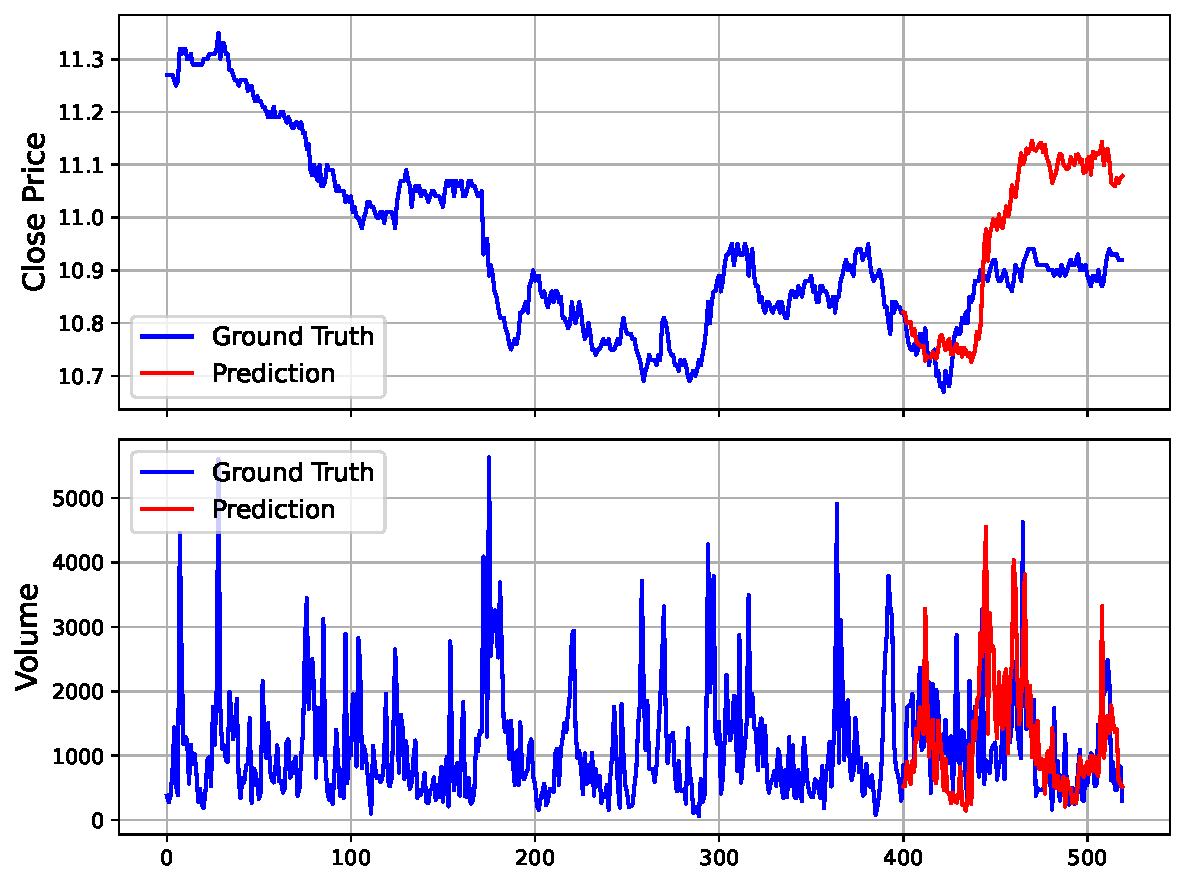
\includegraphics[width=\linewidth]{pred_imgs/pred_visualize_stock_XSHG_600977_5min_Kronos_small.pdf}
        \caption{$\text{Kronos}_{small}$}
    \end{subfigure}
    \hfill
    \begin{subfigure}[b]{0.33\textwidth}
        \centering
        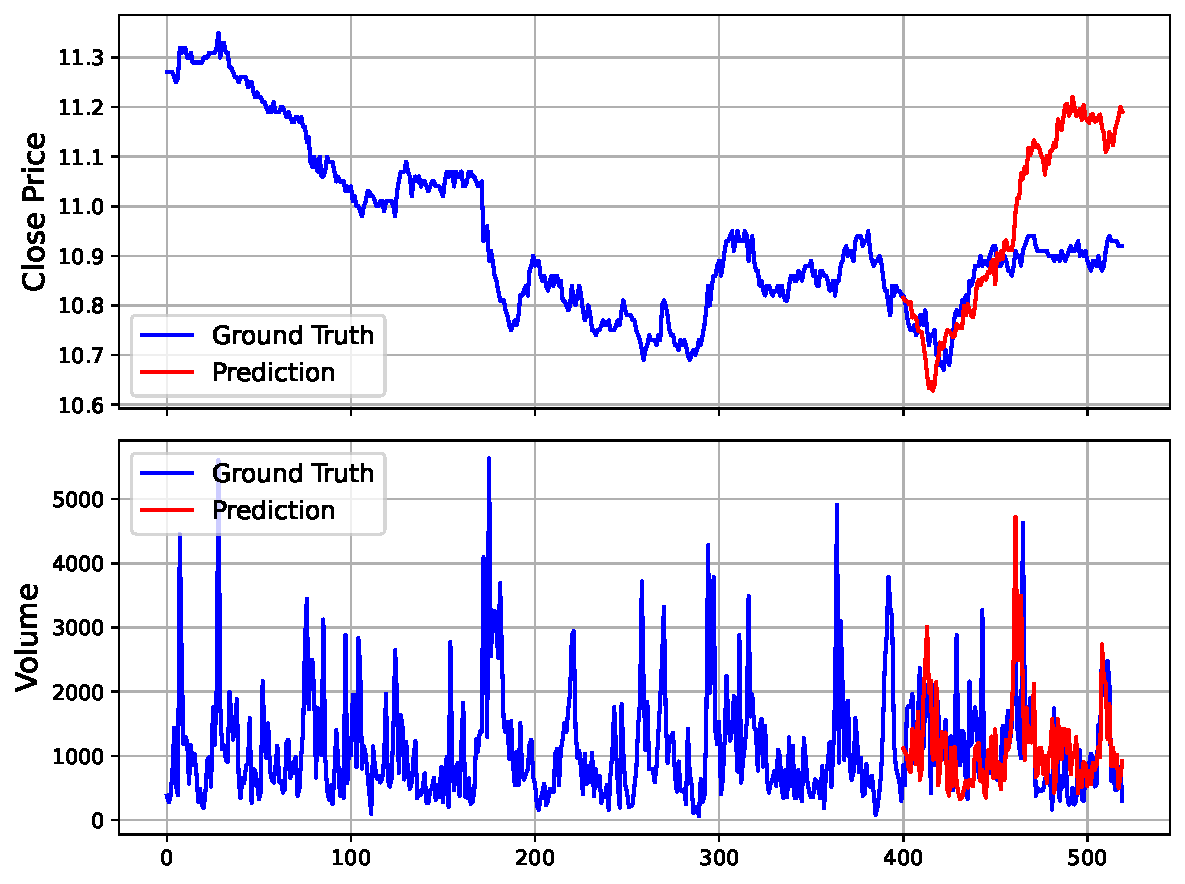
\includegraphics[width=\linewidth]{pred_imgs/pred_visualize_stock_XSHG_600977_5min_Kronos_base.pdf}
        \caption{$\text{Kronos}_{base}$}
    \end{subfigure}
    \hfill
    \begin{subfigure}[b]{0.33\textwidth}
        \centering
        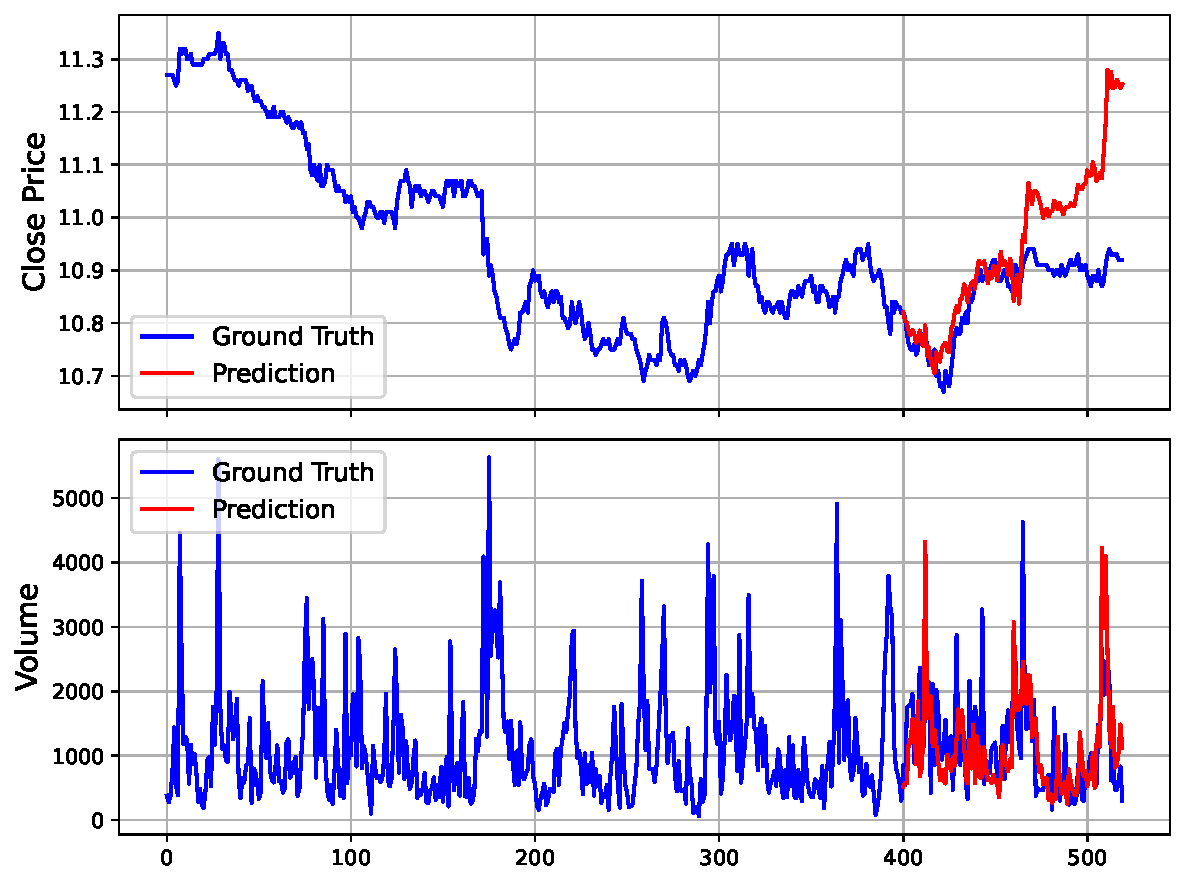
\includegraphics[width=\linewidth]{pred_imgs/pred_visualize_stock_XSHG_600977_5min_Kronos_large.pdf}
        \caption{$\text{Kronos}_{large}$}
    \end{subfigure}

    \vspace{0.1cm}

    \begin{subfigure}[b]{0.33\textwidth}
        \centering
        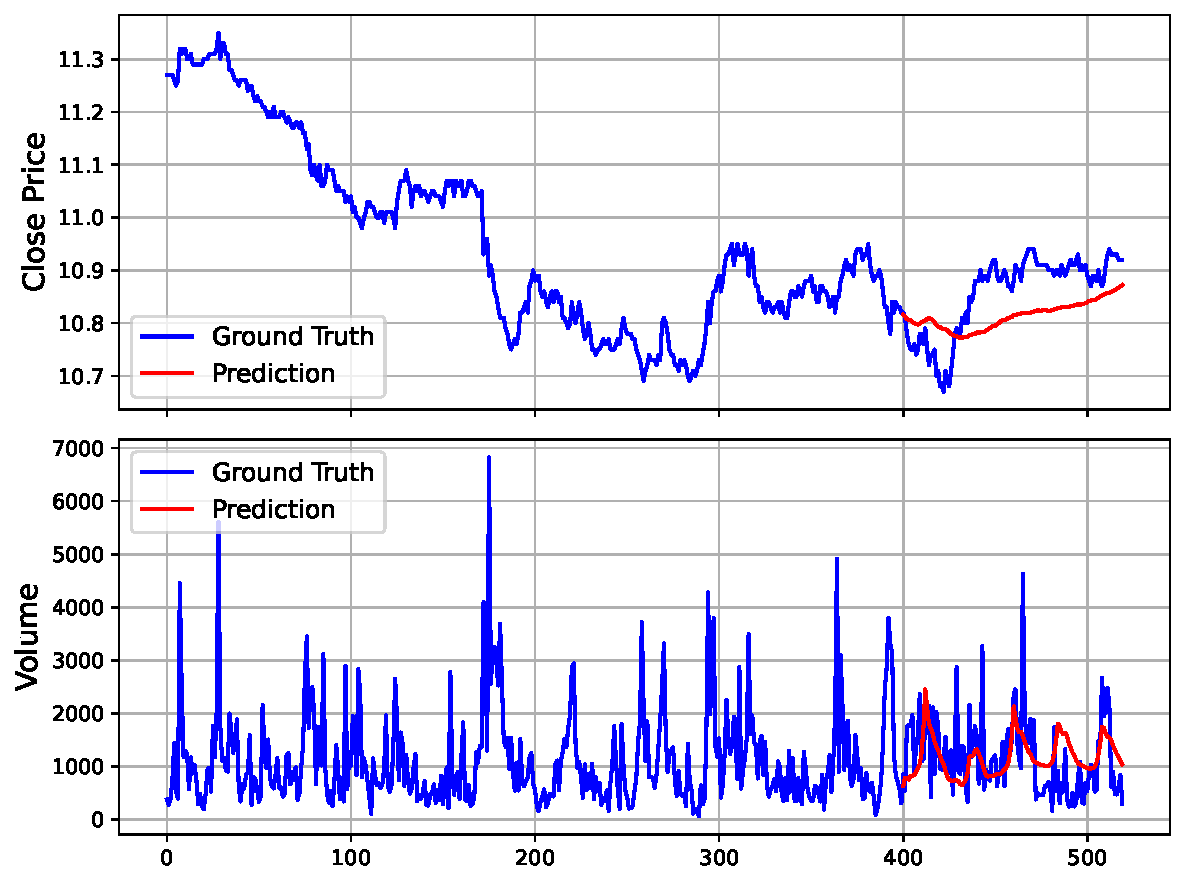
\includegraphics[width=\linewidth]{pred_imgs/pred_visualize_stock_XSHG_600977_5min_TimeMOE_small.pdf}
        \caption{$\text{TimeMOE}_{small}$}
    \end{subfigure}
    \hfill
    \begin{subfigure}[b]{0.33\textwidth}
        \centering
        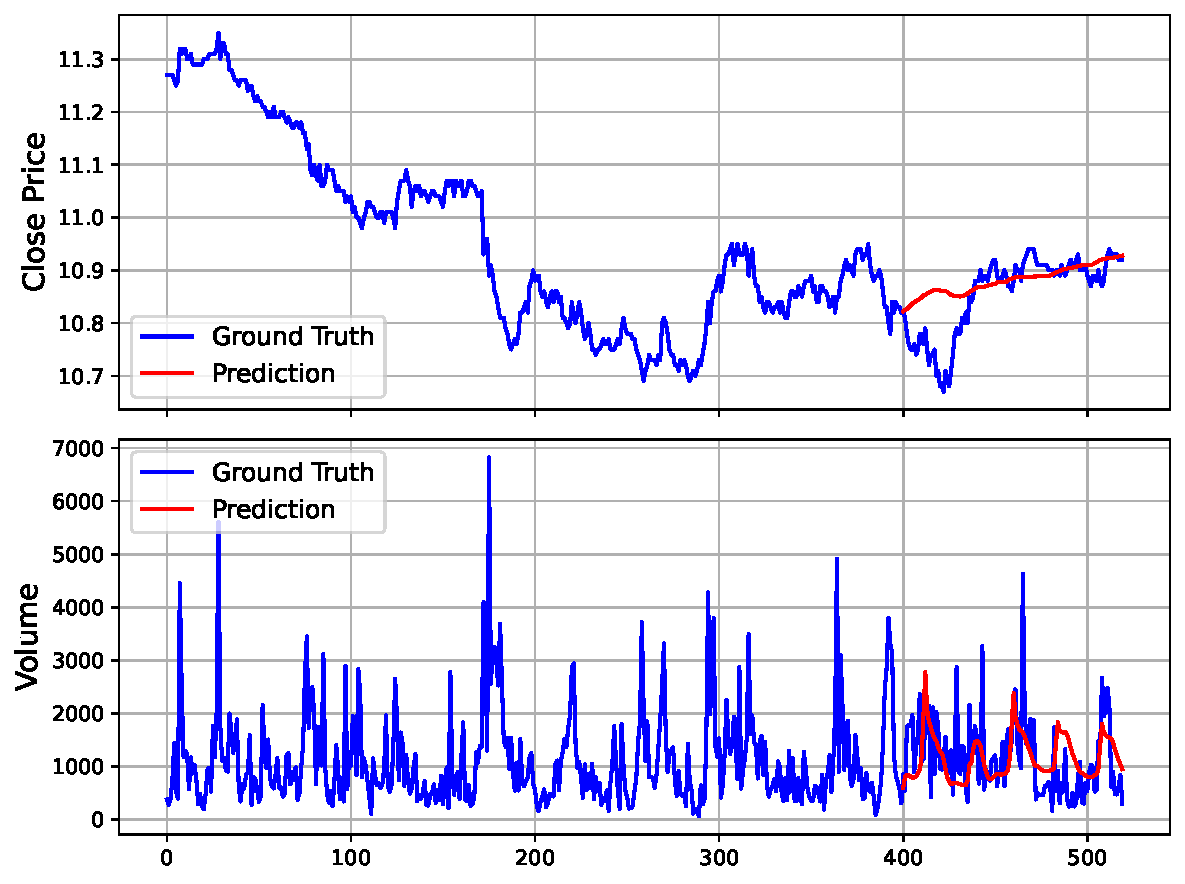
\includegraphics[width=\linewidth]{pred_imgs/pred_visualize_stock_XSHG_600977_5min_TimeMOE_large.pdf}
        \caption{$\text{TimeMOE}_{large}$}
    \end{subfigure}
    \hfill
    \begin{subfigure}[b]{0.33\textwidth}
        \centering
        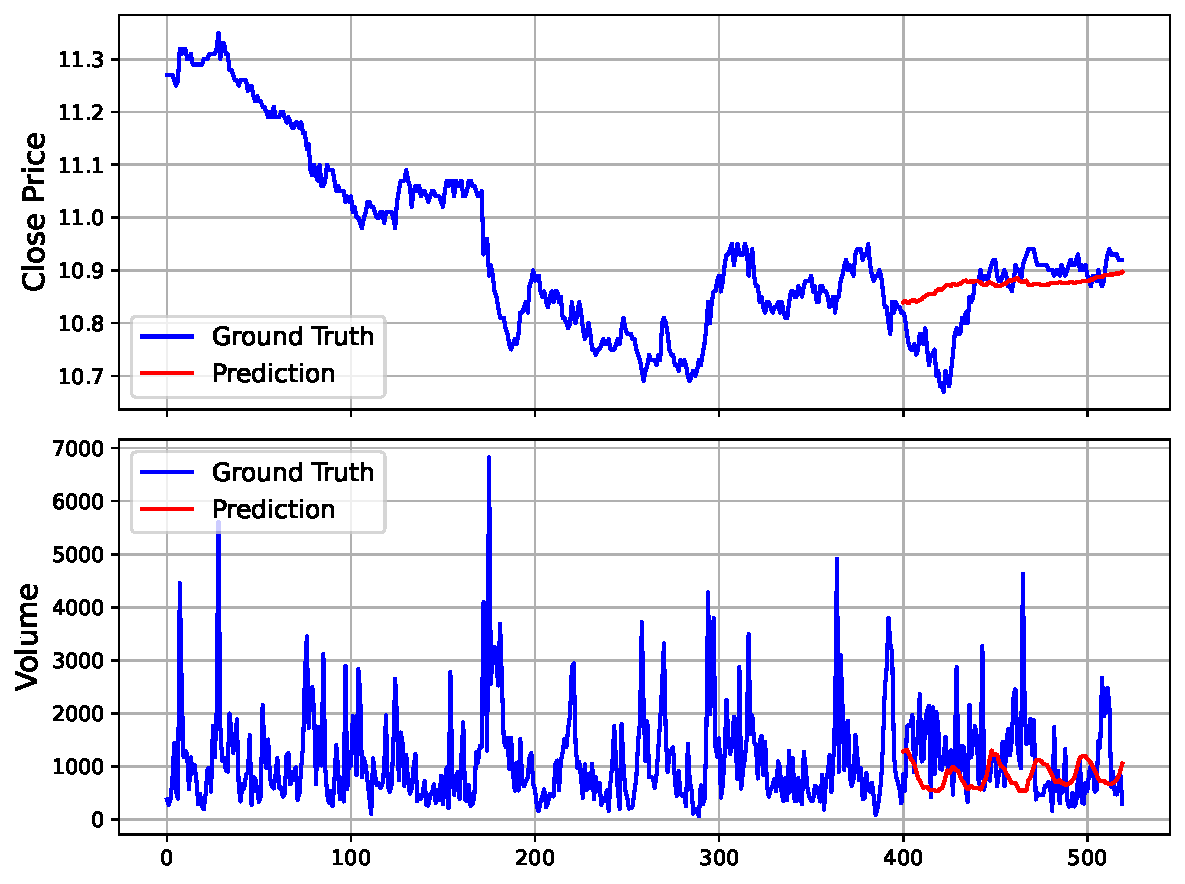
\includegraphics[width=\linewidth]{pred_imgs/pred_visualize_stock_XSHG_600977_5min_TimesFM.pdf}
        \caption{TimesFM}
    \end{subfigure}

    \vspace{0.1cm}

    \begin{subfigure}[b]{0.33\textwidth}
        \centering
        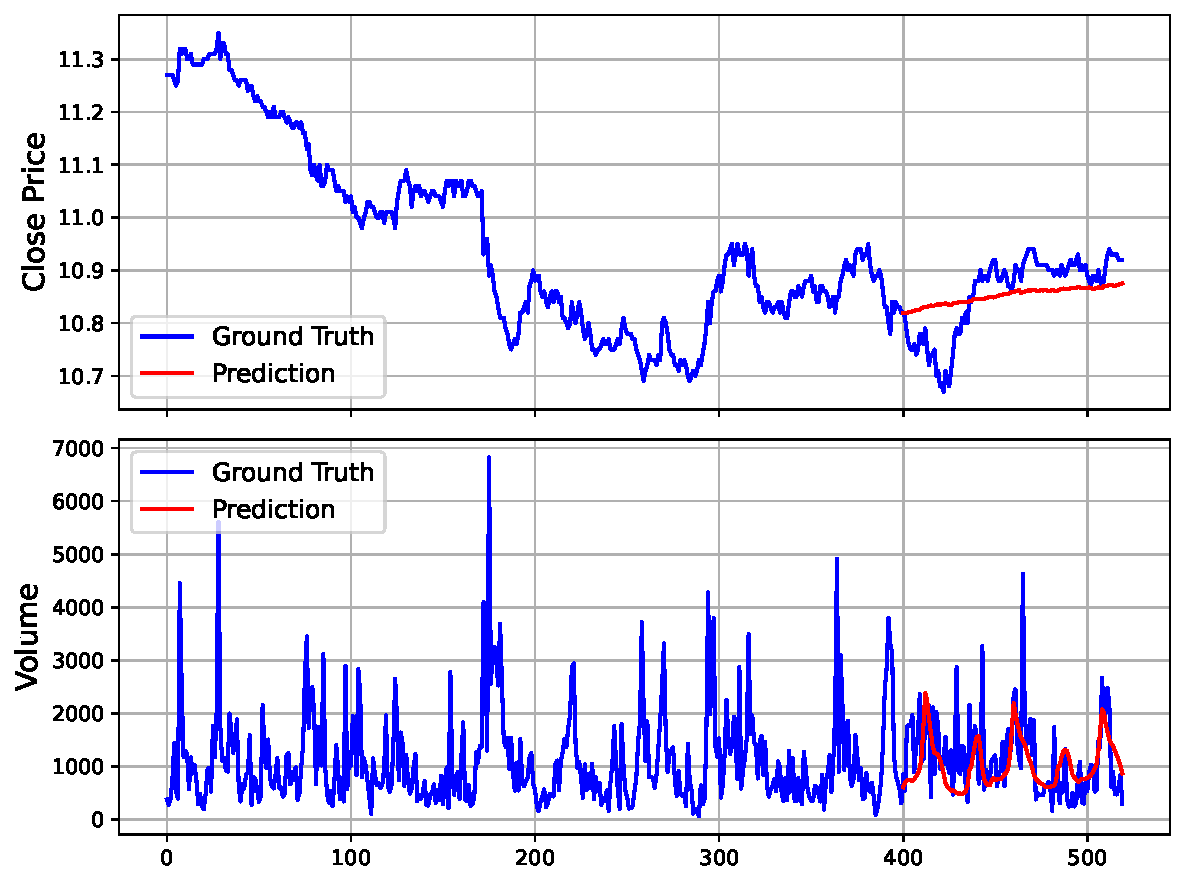
\includegraphics[width=\linewidth]{pred_imgs/pred_visualize_stock_XSHG_600977_5min_Chronos_small.pdf}
        \caption{$\text{Chronos}_{small}$}
    \end{subfigure}
    \hfill
    \begin{subfigure}[b]{0.33\textwidth}
        \centering
        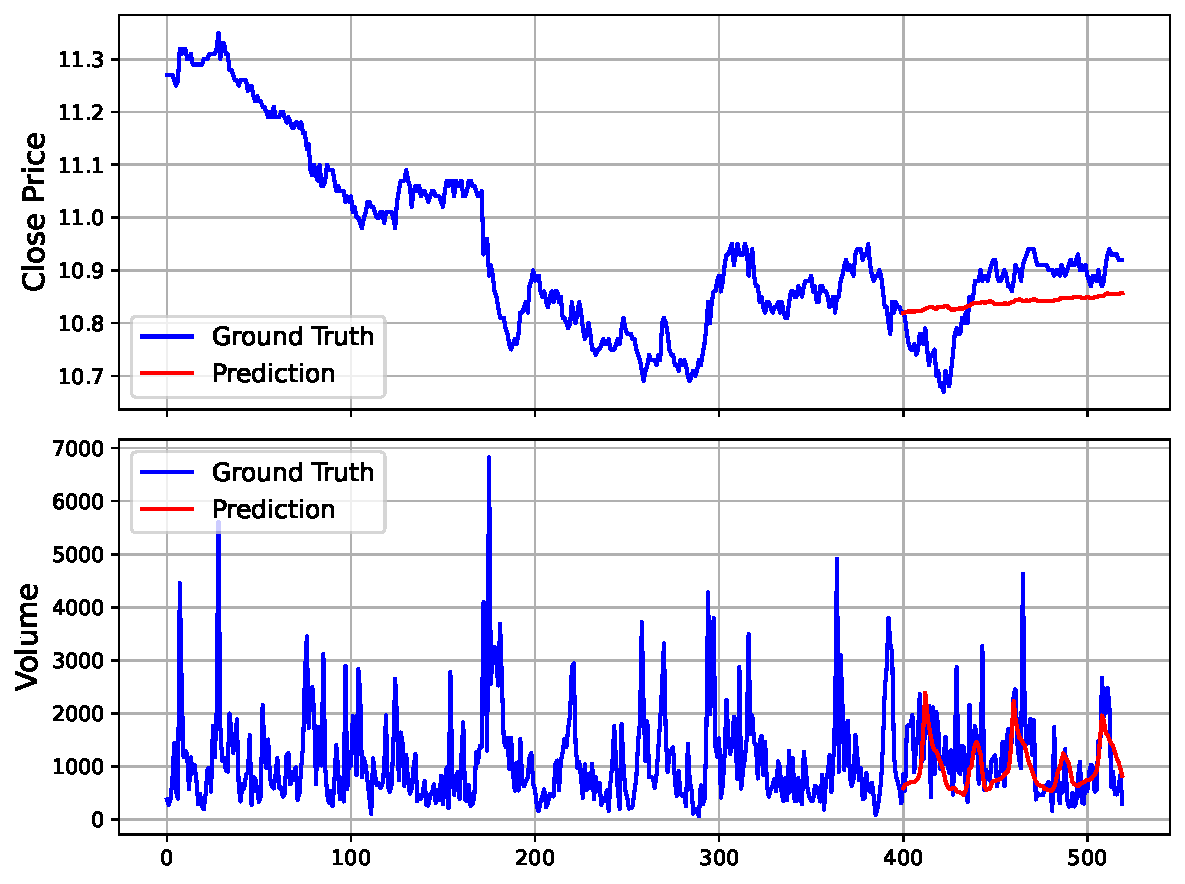
\includegraphics[width=\linewidth]{pred_imgs/pred_visualize_stock_XSHG_600977_5min_Chronos_base.pdf}
        \caption{$\text{Chronos}_{base}$}
    \end{subfigure}
    \hfill
    \begin{subfigure}[b]{0.33\textwidth}
        \centering
        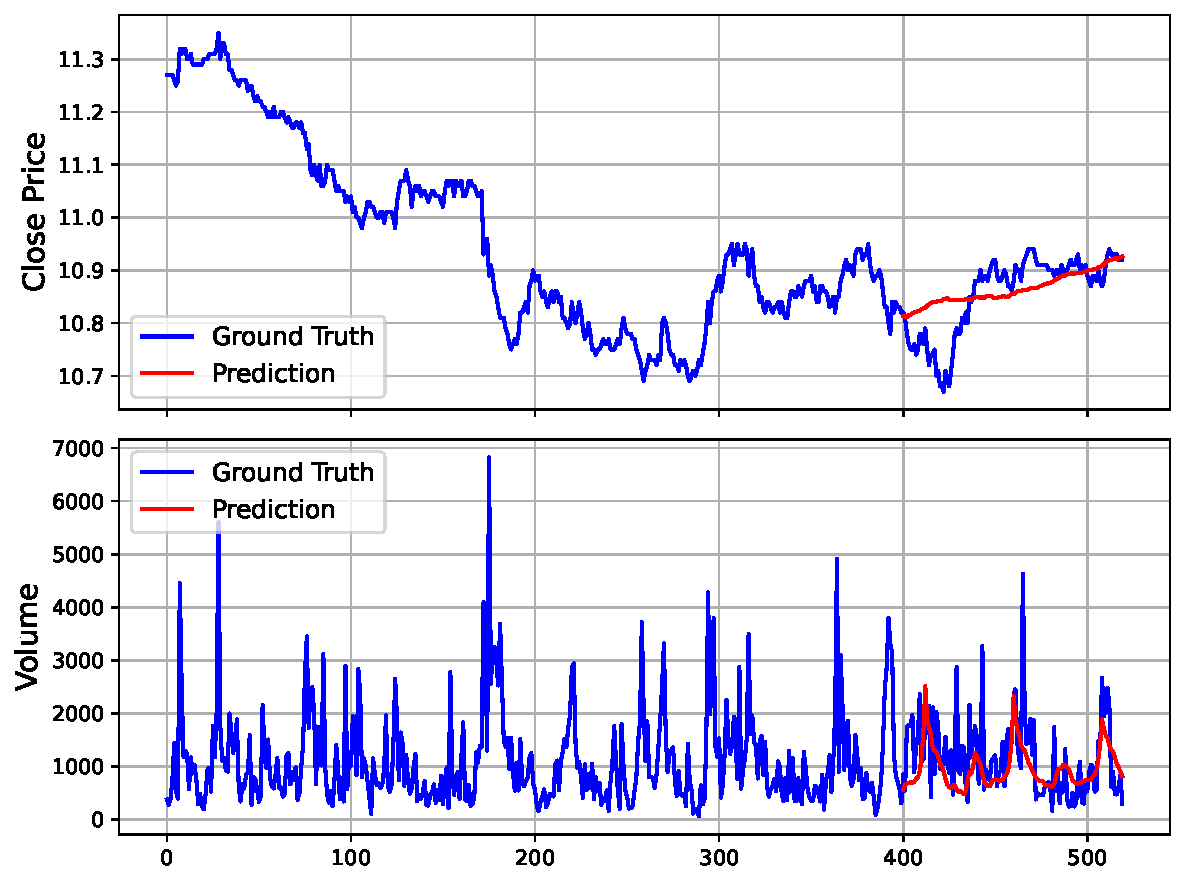
\includegraphics[width=\linewidth]{pred_imgs/pred_visualize_stock_XSHG_600977_5min_Chronos_large.pdf}
        \caption{$\text{Chronos}_{large}$}
    \end{subfigure}

    \vspace{0.1cm}

    \begin{subfigure}[b]{0.33\textwidth}
        \centering
        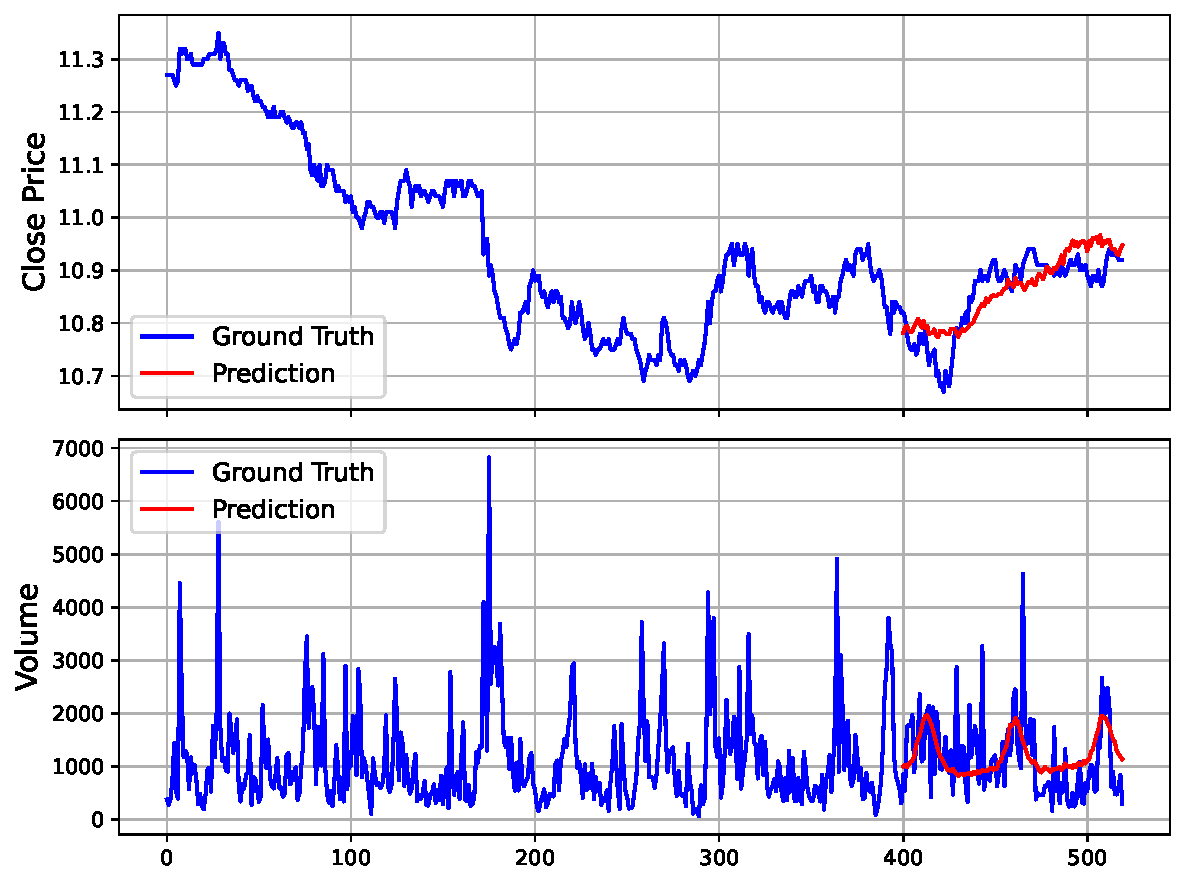
\includegraphics[width=\linewidth]{pred_imgs/pred_visualize_stock_XSHG_600977_5min_iTransformer.pdf}
        \caption{iTransformer}
    \end{subfigure}
    \hfill
    \begin{subfigure}[b]{0.33\textwidth}
        \centering
        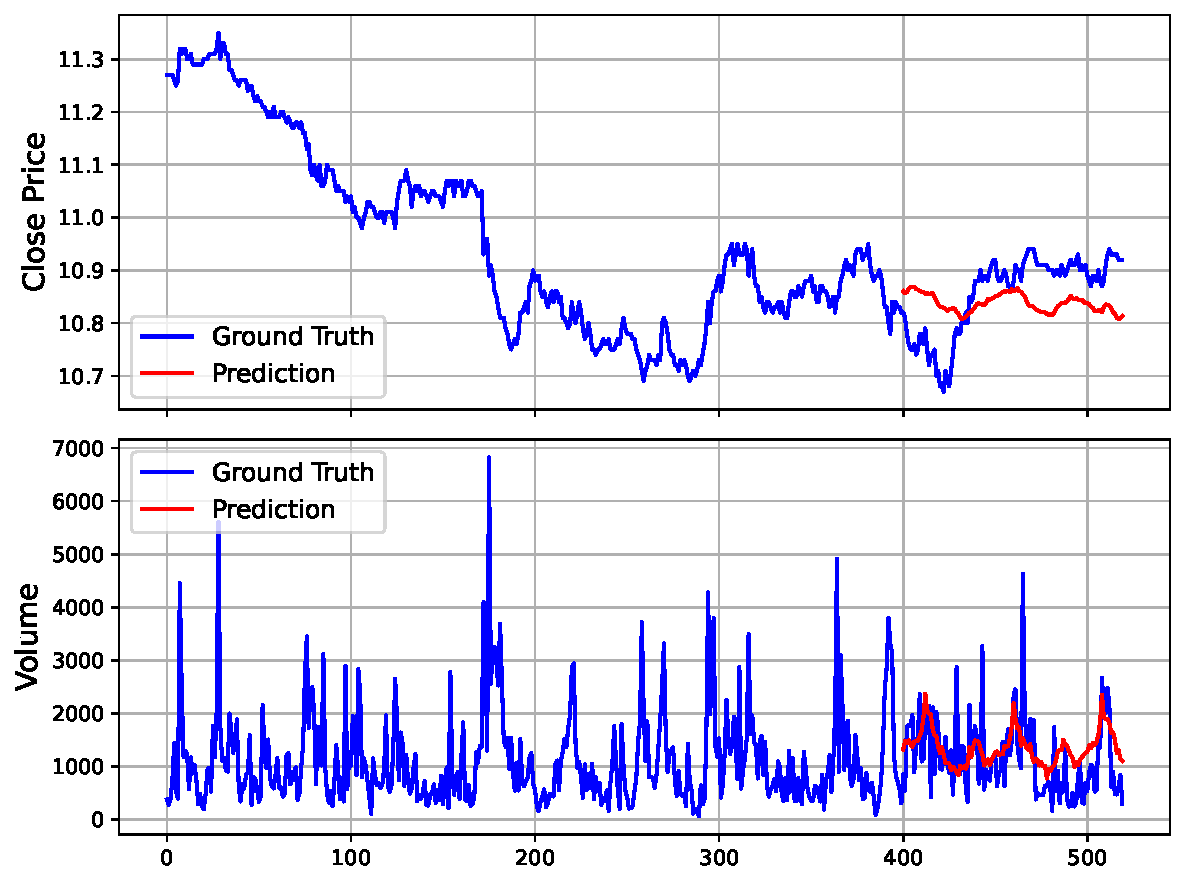
\includegraphics[width=\linewidth]{pred_imgs/pred_visualize_stock_XSHG_600977_5min_DLinear.pdf}
        \caption{DLinear}
    \end{subfigure}
    \hfill
    \begin{subfigure}[b]{0.33\textwidth}
        \centering
        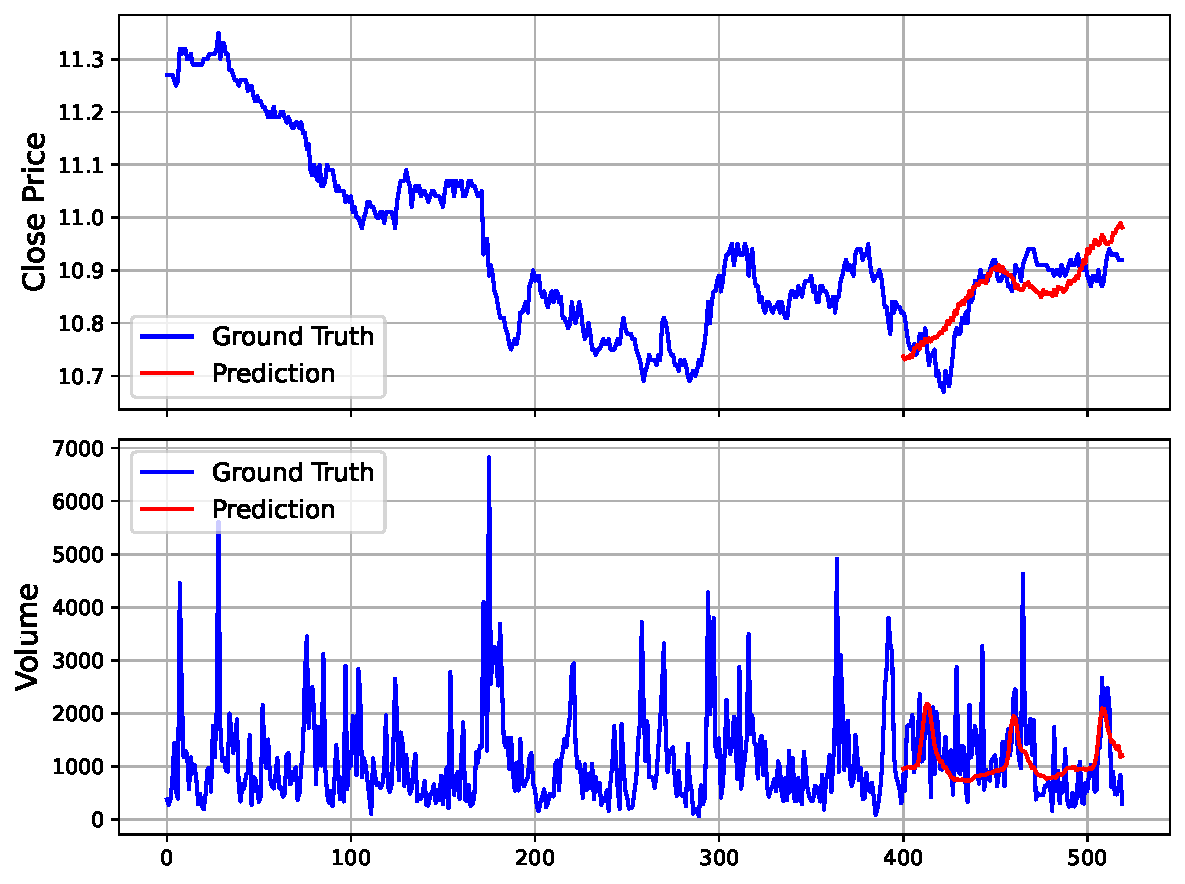
\includegraphics[width=\linewidth]{pred_imgs/pred_visualize_stock_XSHG_600977_5min_TimesNet.pdf}
        \caption{TimesNet}
    \end{subfigure}

    \caption{5분 K-line 데이터를 기반으로 한 China Film Co.,Ltd. (SSE: 600977)의 `Close Price'와 `Volume' 예측 결과. 모델은 400스텝 look-back 윈도우를 사용하여 120스텝 horizon을 예측한다. \textcolor{blue}{Blue} 선은 정답값을 나타내고 \textcolor{red}{red} 선은 모델의 예측값을 나타낸다.}
    \label{fig:pred_case_1}
\end{figure*}

\begin{figure*}[ht]
    \centering

    \begin{subfigure}[b]{0.33\textwidth}
        \centering
        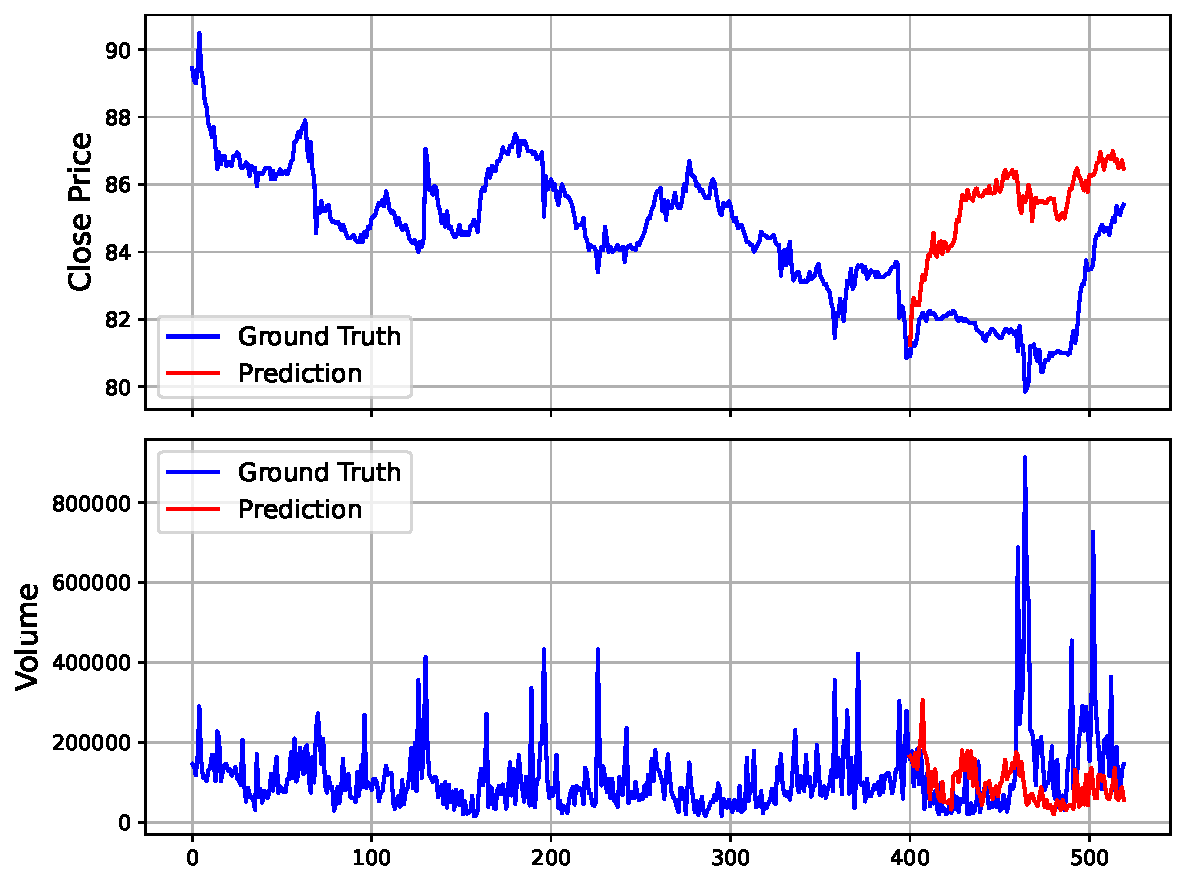
\includegraphics[width=\linewidth]{pred_imgs/pred_visualize_stock_XHKG_9992_5min_Kronos_small.pdf}
        \caption{$\text{Kronos}_{small}$}
    \end{subfigure}
    \hfill
    \begin{subfigure}[b]{0.33\textwidth}
        \centering
        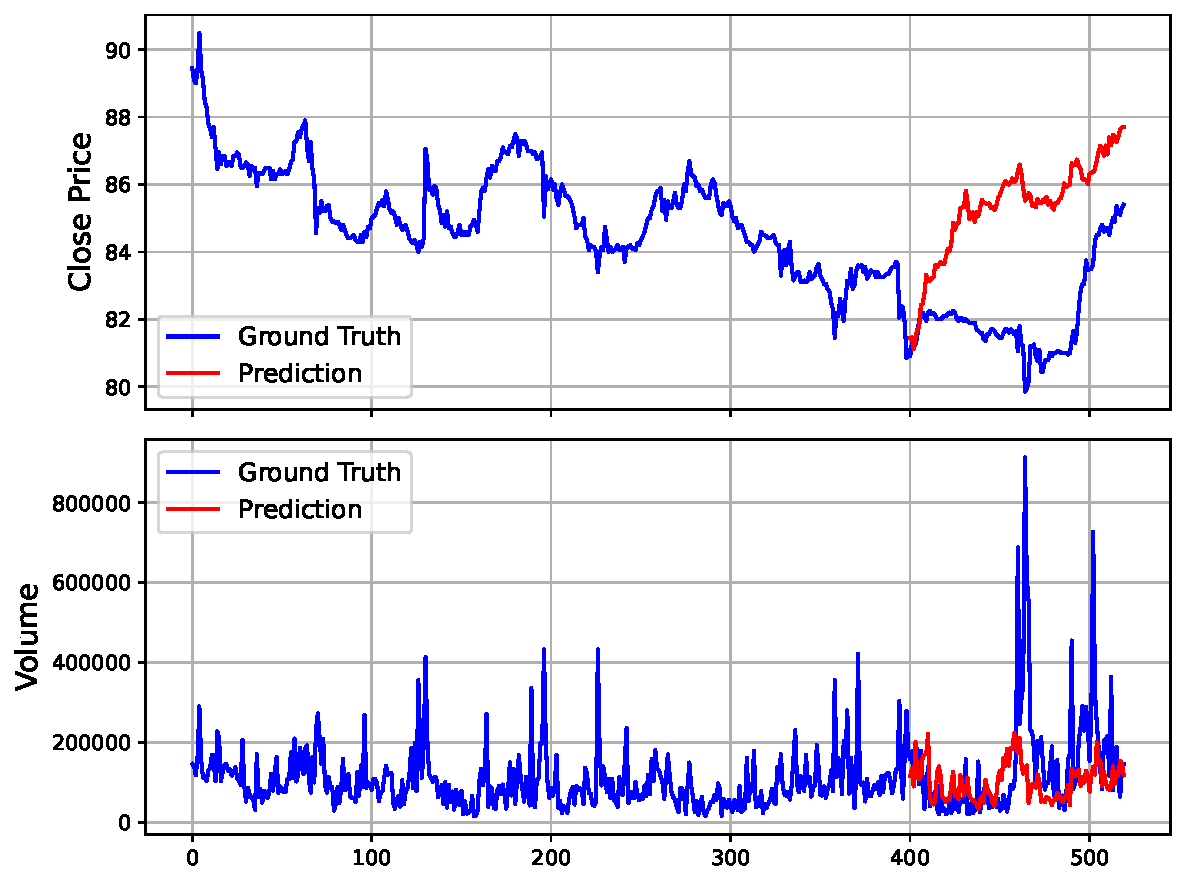
\includegraphics[width=\linewidth]{pred_imgs/pred_visualize_stock_XHKG_9992_5min_Kronos_base.pdf}
        \caption{$\text{Kronos}_{base}$}
    \end{subfigure}
    \hfill
    \begin{subfigure}[b]{0.33\textwidth}
        \centering
        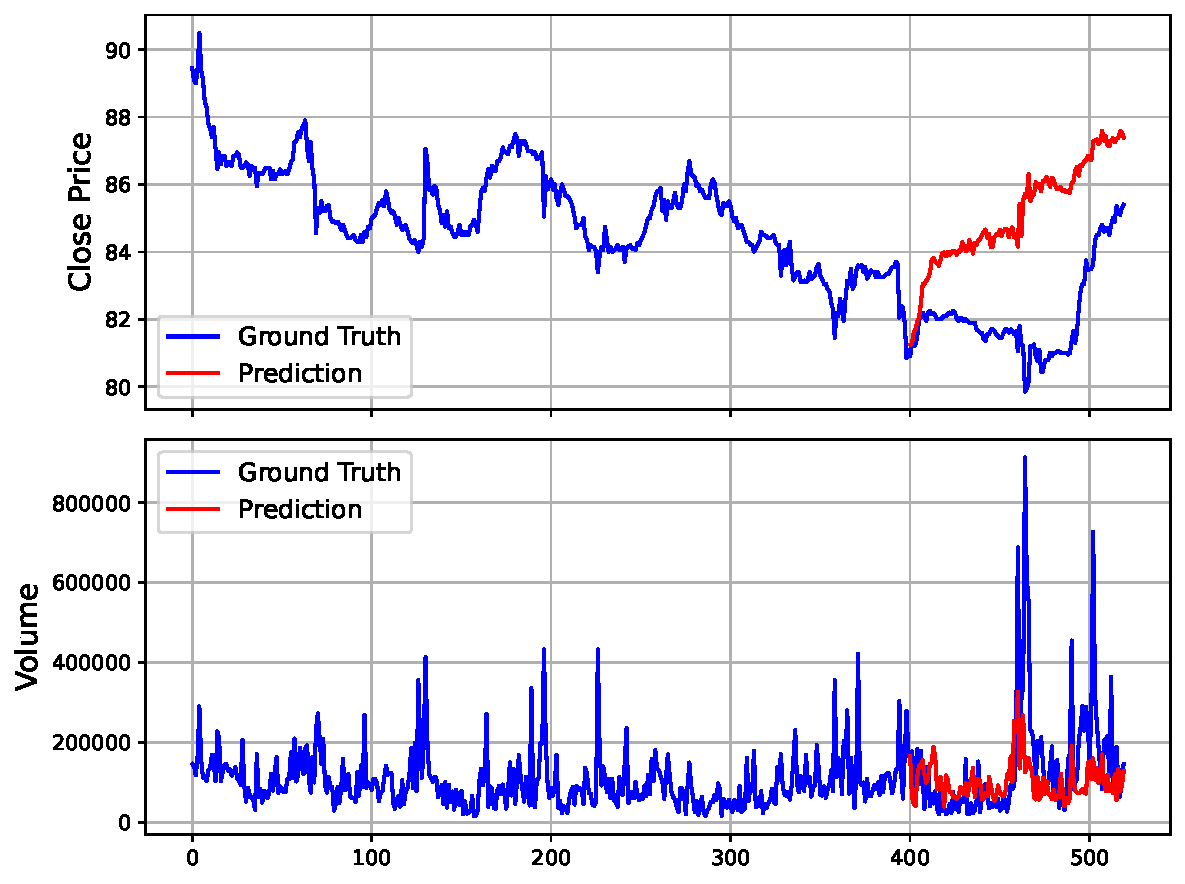
\includegraphics[width=\linewidth]{pred_imgs/pred_visualize_stock_XHKG_9992_5min_Kronos_large.pdf}
        \caption{$\text{Kronos}_{large}$}
    \end{subfigure}

    \vspace{0.1cm}

    \begin{subfigure}[b]{0.33\textwidth}
        \centering
        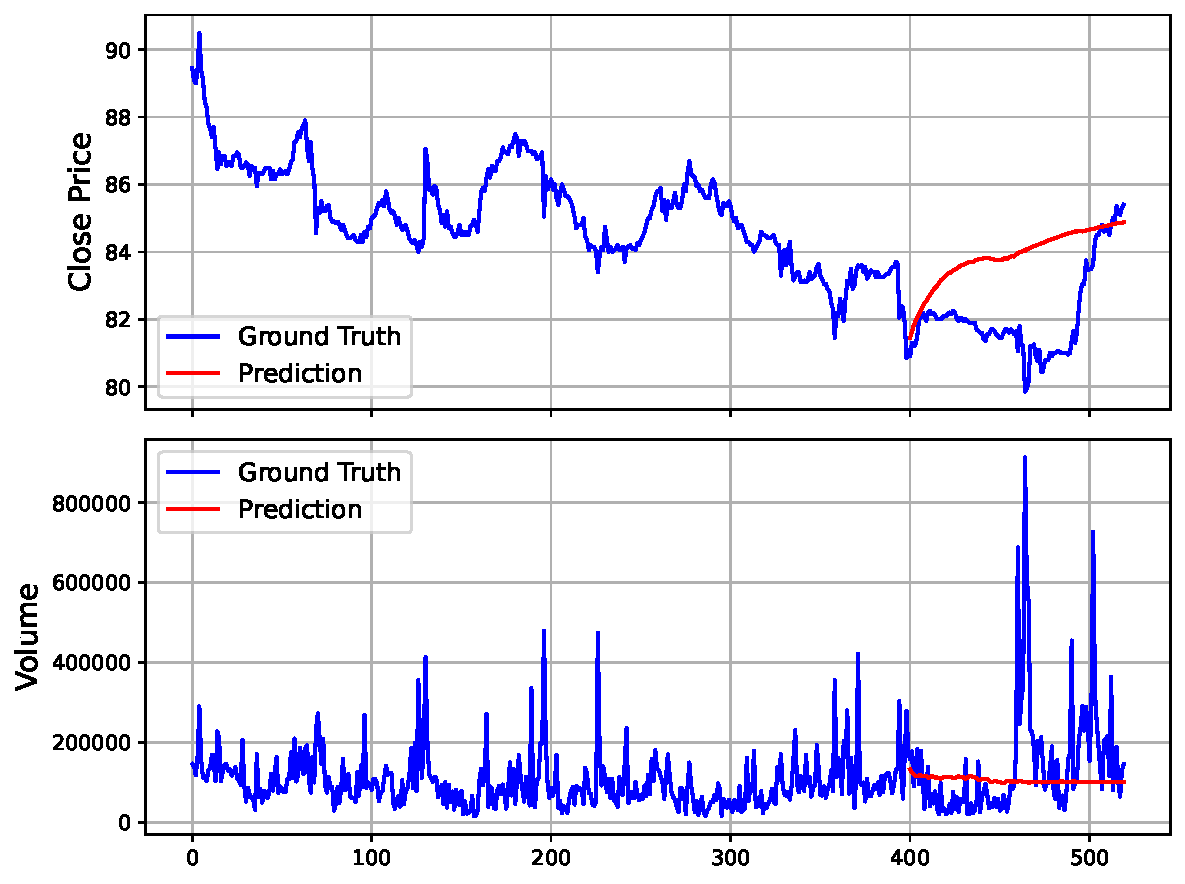
\includegraphics[width=\linewidth]{pred_imgs/pred_visualize_stock_XHKG_9992_5min_TimeMOE_small.pdf}
        \caption{$\text{TimeMOE}_{small}$}
    \end{subfigure}
    \hfill
    \begin{subfigure}[b]{0.33\textwidth}
        \centering
        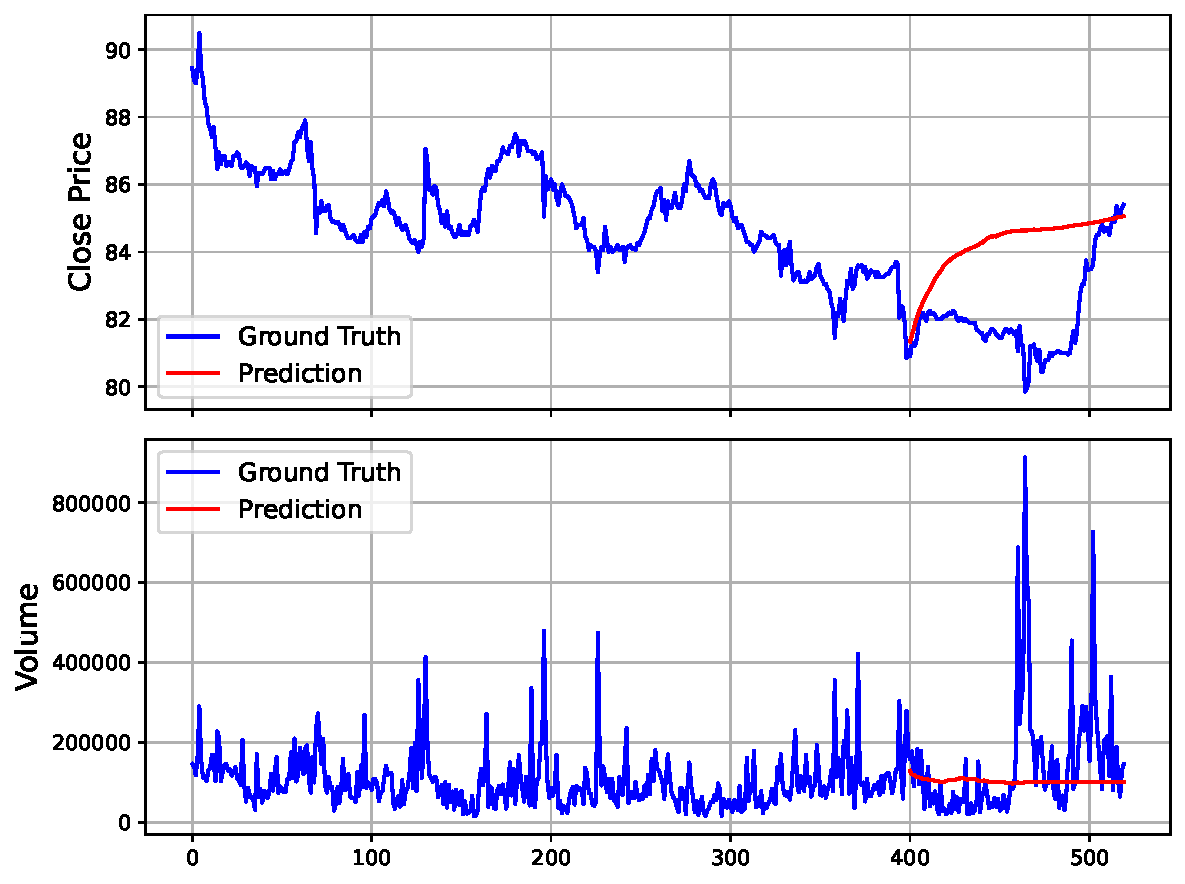
\includegraphics[width=\linewidth]{pred_imgs/pred_visualize_stock_XHKG_9992_5min_TimeMOE_large.pdf}
        \caption{$\text{TimeMOE}_{large}$}
    \end{subfigure}
    \hfill
    \begin{subfigure}[b]{0.33\textwidth}
        \centering
        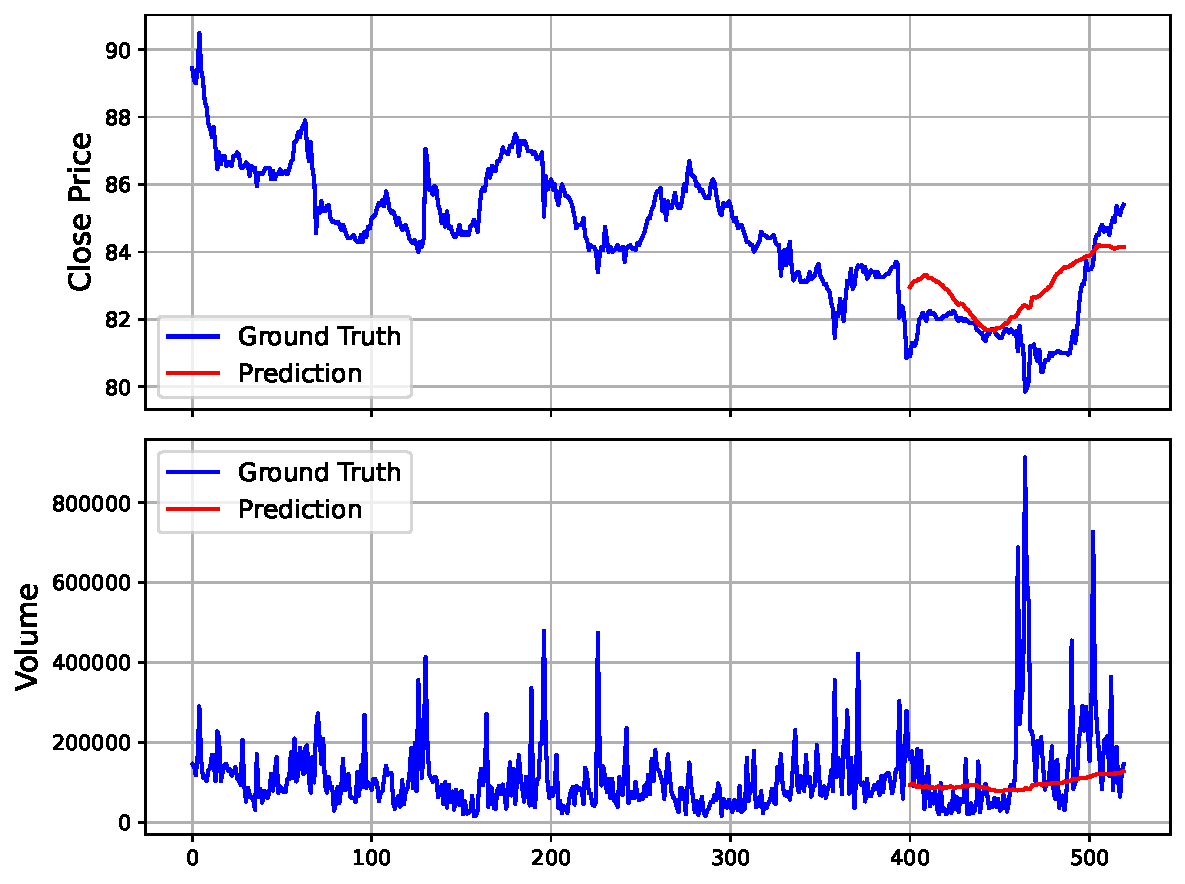
\includegraphics[width=\linewidth]{pred_imgs/pred_visualize_stock_XHKG_9992_5min_TimesFM.pdf}
        \caption{TimesFM}
    \end{subfigure}

    \vspace{0.1cm}

    \begin{subfigure}[b]{0.33\textwidth}
        \centering
        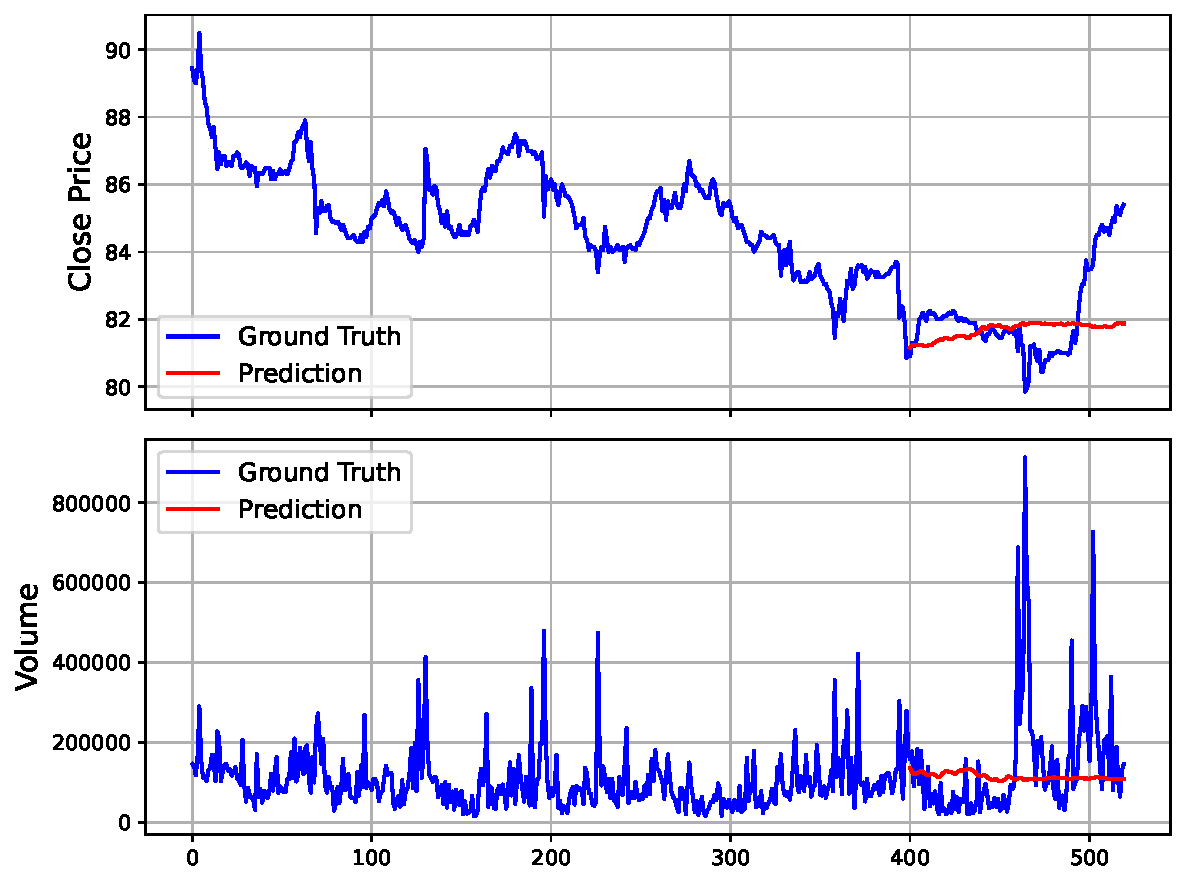
\includegraphics[width=\linewidth]{pred_imgs/pred_visualize_stock_XHKG_9992_5min_Chronos_small.pdf}
        \caption{$\text{Chronos}_{small}$}
    \end{subfigure}
    \hfill
    \begin{subfigure}[b]{0.33\textwidth}
        \centering
        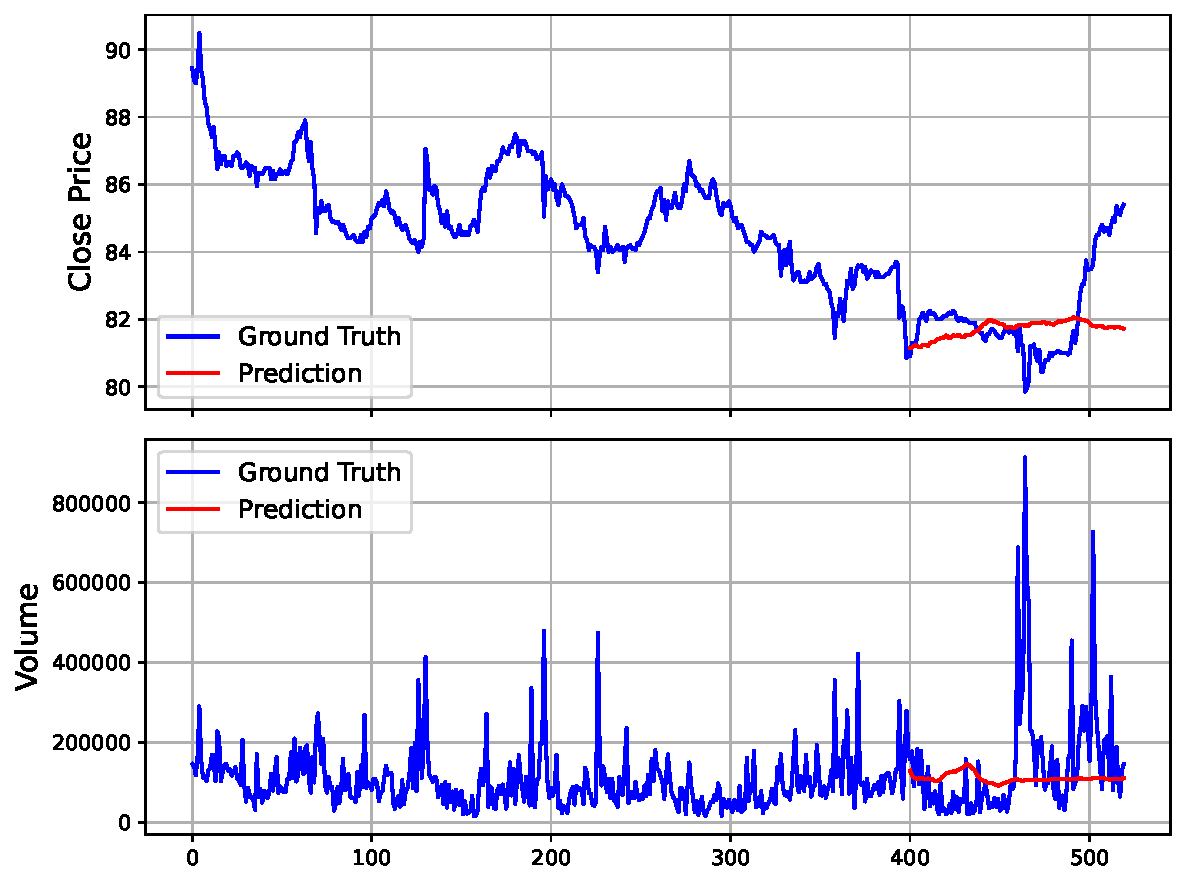
\includegraphics[width=\linewidth]{pred_imgs/pred_visualize_stock_XHKG_9992_5min_Chronos_base.pdf}
        \caption{$\text{Chronos}_{base}$}
    \end{subfigure}
    \hfill
    \begin{subfigure}[b]{0.33\textwidth}
        \centering
        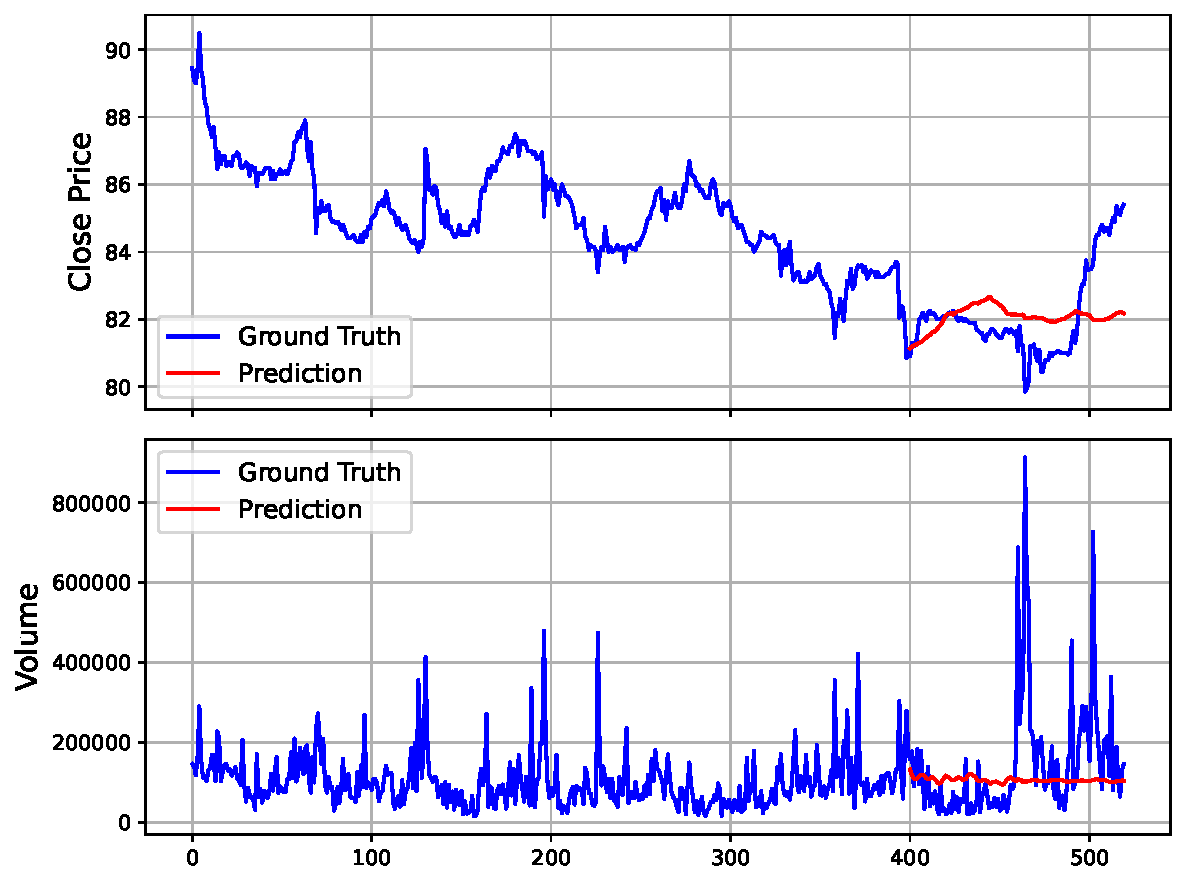
\includegraphics[width=\linewidth]{pred_imgs/pred_visualize_stock_XHKG_9992_5min_Chronos_large.pdf}
        \caption{$\text{Chronos}_{large}$}
    \end{subfigure}

    \vspace{0.1cm}

    \begin{subfigure}[b]{0.33\textwidth}
        \centering
        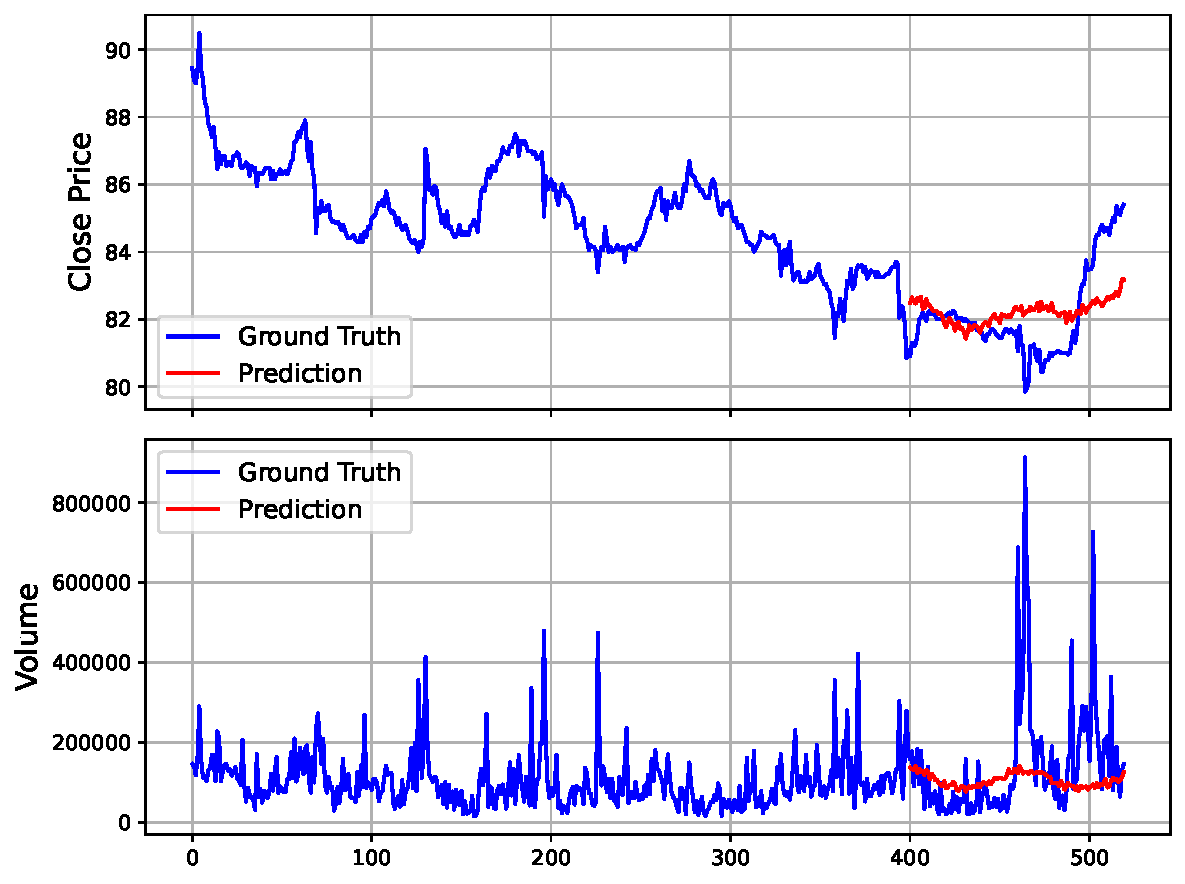
\includegraphics[width=\linewidth]{pred_imgs/pred_visualize_stock_XHKG_9992_5min_iTransformer.pdf}
        \caption{iTransformer}
    \end{subfigure}
    \hfill
    \begin{subfigure}[b]{0.33\textwidth}
        \centering
        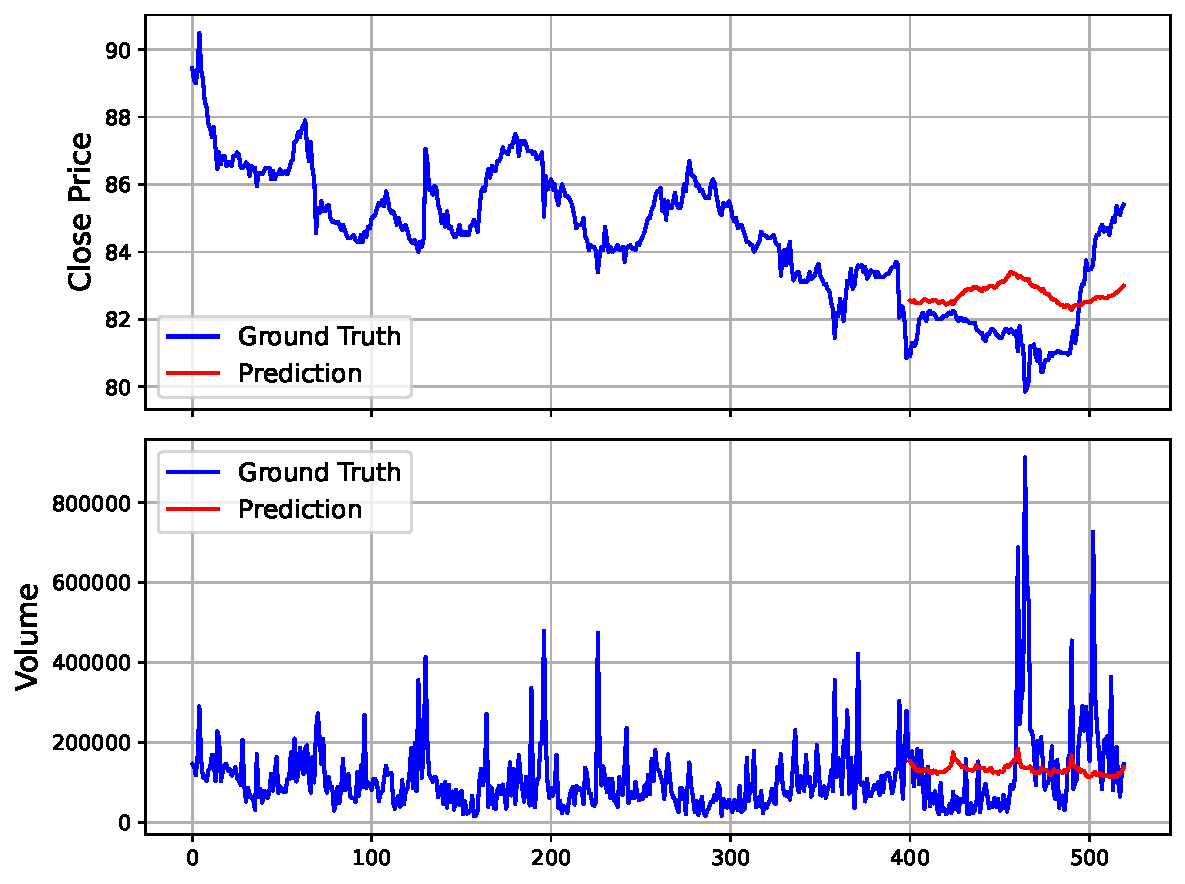
\includegraphics[width=\linewidth]{pred_imgs/pred_visualize_stock_XHKG_9992_5min_DLinear.pdf}
        \caption{DLinear}
    \end{subfigure}
    \hfill
    \begin{subfigure}[b]{0.33\textwidth}
        \centering
        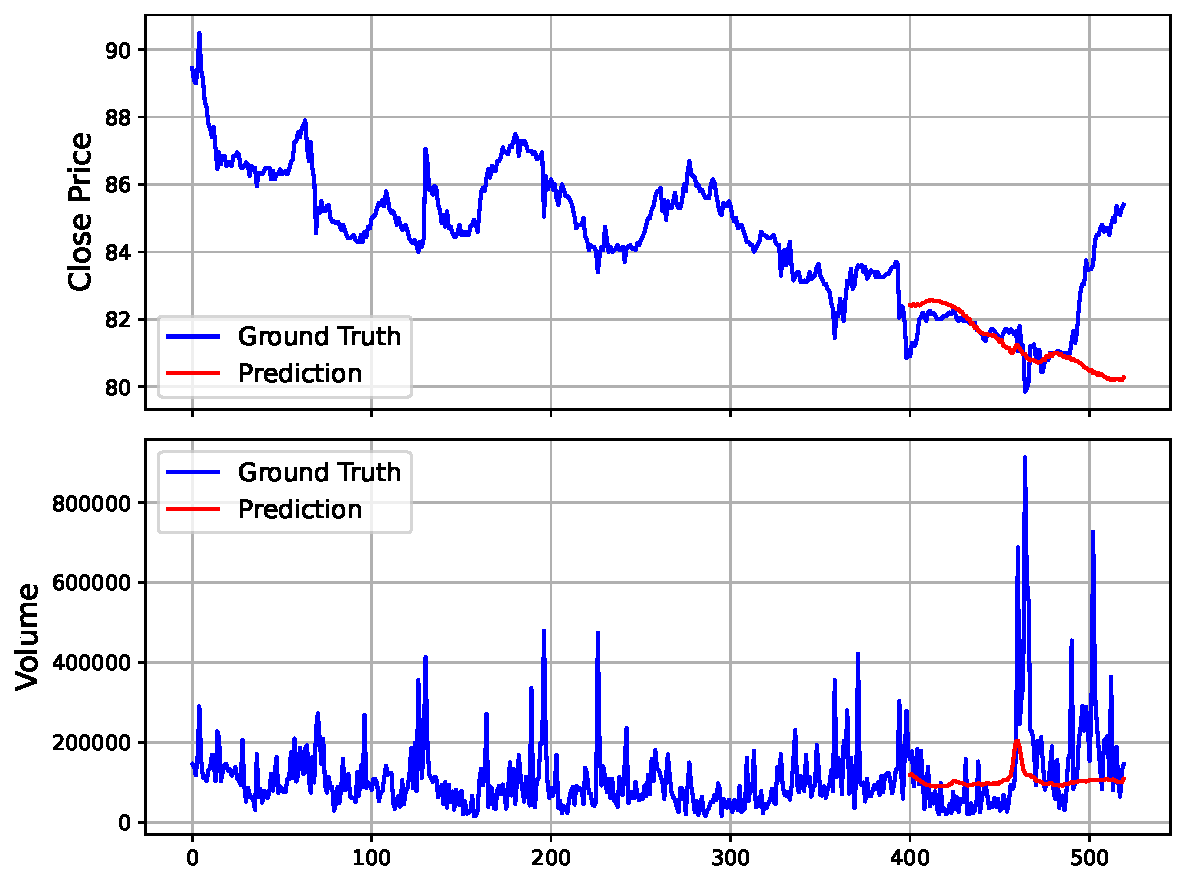
\includegraphics[width=\linewidth]{pred_imgs/pred_visualize_stock_XHKG_9992_5min_TimesNet.pdf}
        \caption{TimesNet}
    \end{subfigure}

    \caption{5분 K-line 데이터를 기반으로 한 Pop Mart (HKEX: 09992)의 `Close Price'와 `Volume' 예측 결과. 모델은 400스텝 look-back 윈도우를 사용하여 120스텝 horizon을 예측한다. \textcolor{blue}{Blue} 선은 정답값을 나타내고 \textcolor{red}{red} 선은 모델의 예측값을 나타낸다.}
    \label{fig:pred_case_2}
\end{figure*}


\begin{figure*}[ht]
    \centering

    \begin{subfigure}[b]{0.33\textwidth}
        \centering
        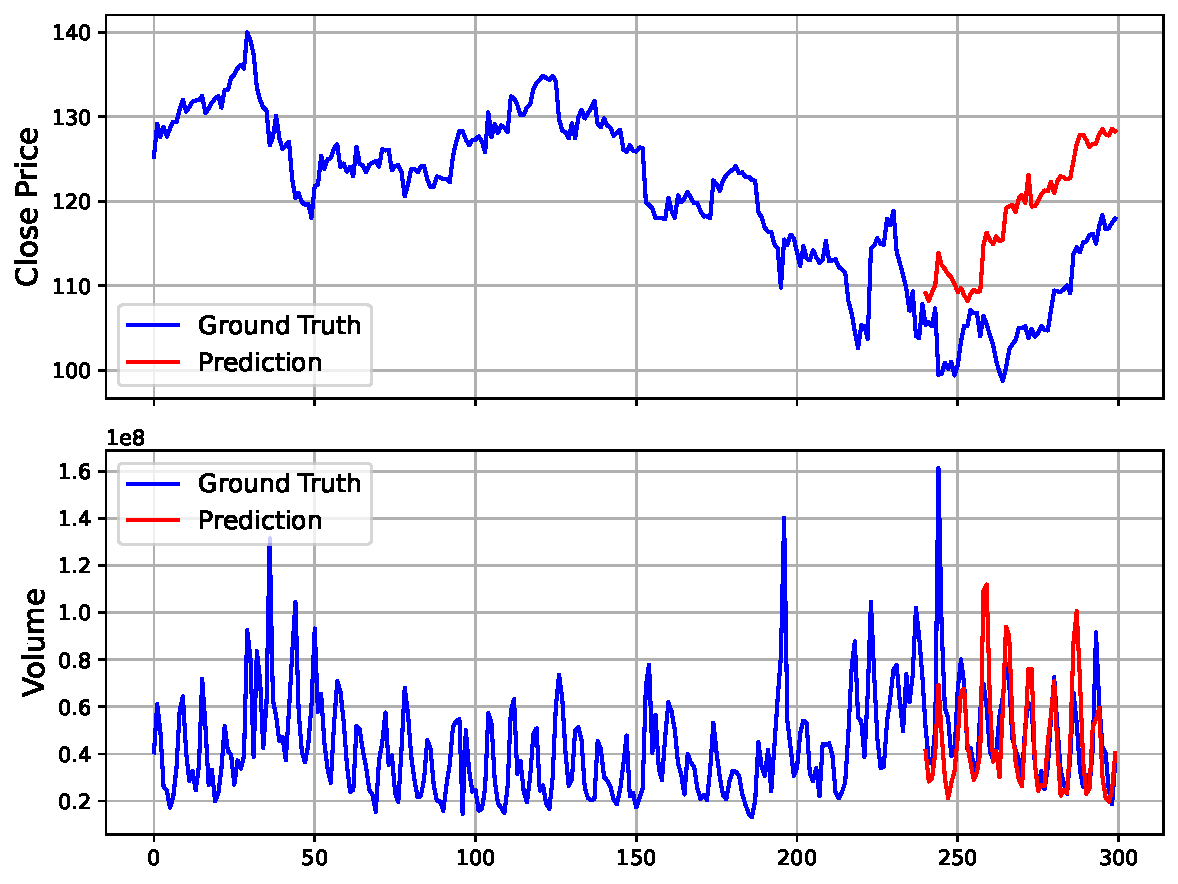
\includegraphics[width=\linewidth]{pred_imgs/pred_visualize_stock_XNAS_NVDA_60min_Kronos_small.pdf}
        \caption{$\text{Kronos}_{small}$}
    \end{subfigure}
    \hfill
    \begin{subfigure}[b]{0.33\textwidth}
        \centering
        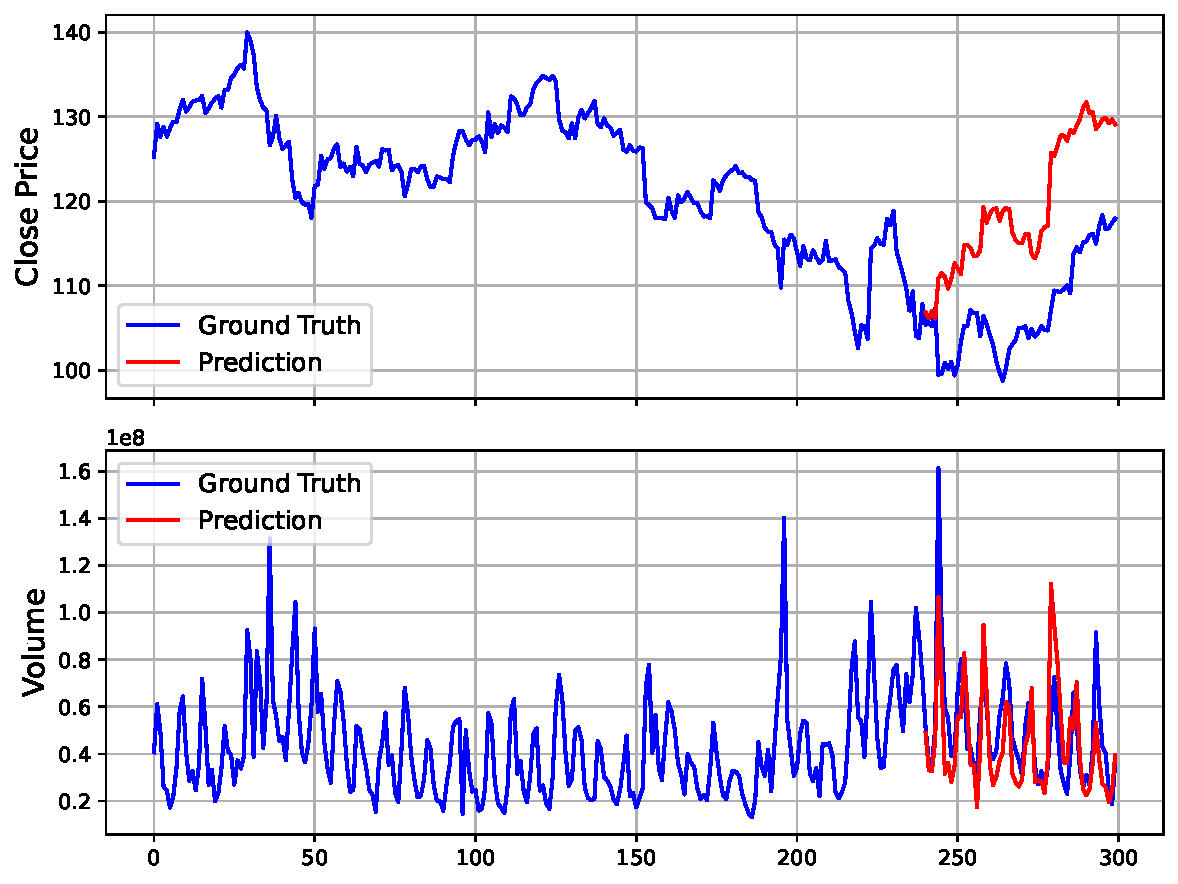
\includegraphics[width=\linewidth]{pred_imgs/pred_visualize_stock_XNAS_NVDA_60min_Kronos_base.pdf}
        \caption{$\text{Kronos}_{base}$}
    \end{subfigure}
    \hfill
    \begin{subfigure}[b]{0.33\textwidth}
        \centering
        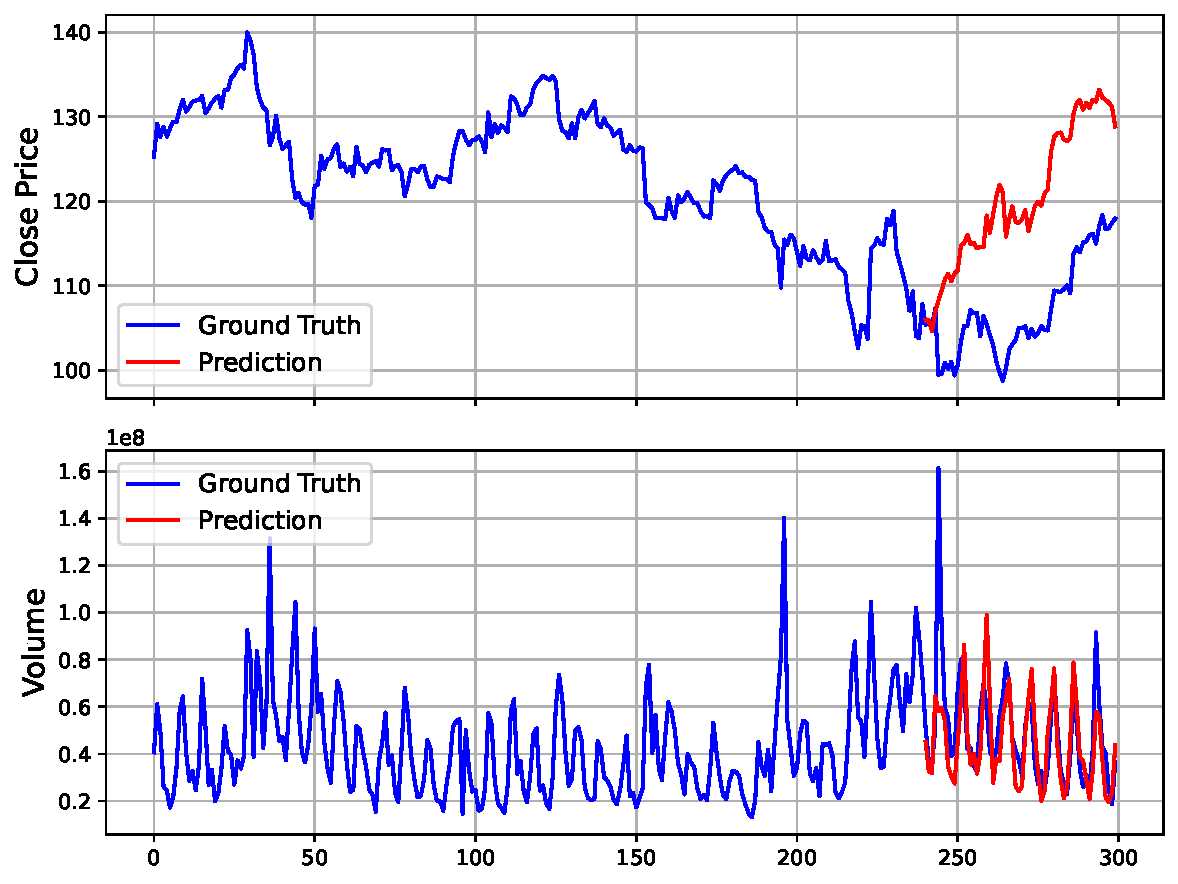
\includegraphics[width=\linewidth]{pred_imgs/pred_visualize_stock_XNAS_NVDA_60min_Kronos_large.pdf}
        \caption{$\text{Kronos}_{large}$}
    \end{subfigure}

    \vspace{0.1cm}

    \begin{subfigure}[b]{0.33\textwidth}
        \centering
        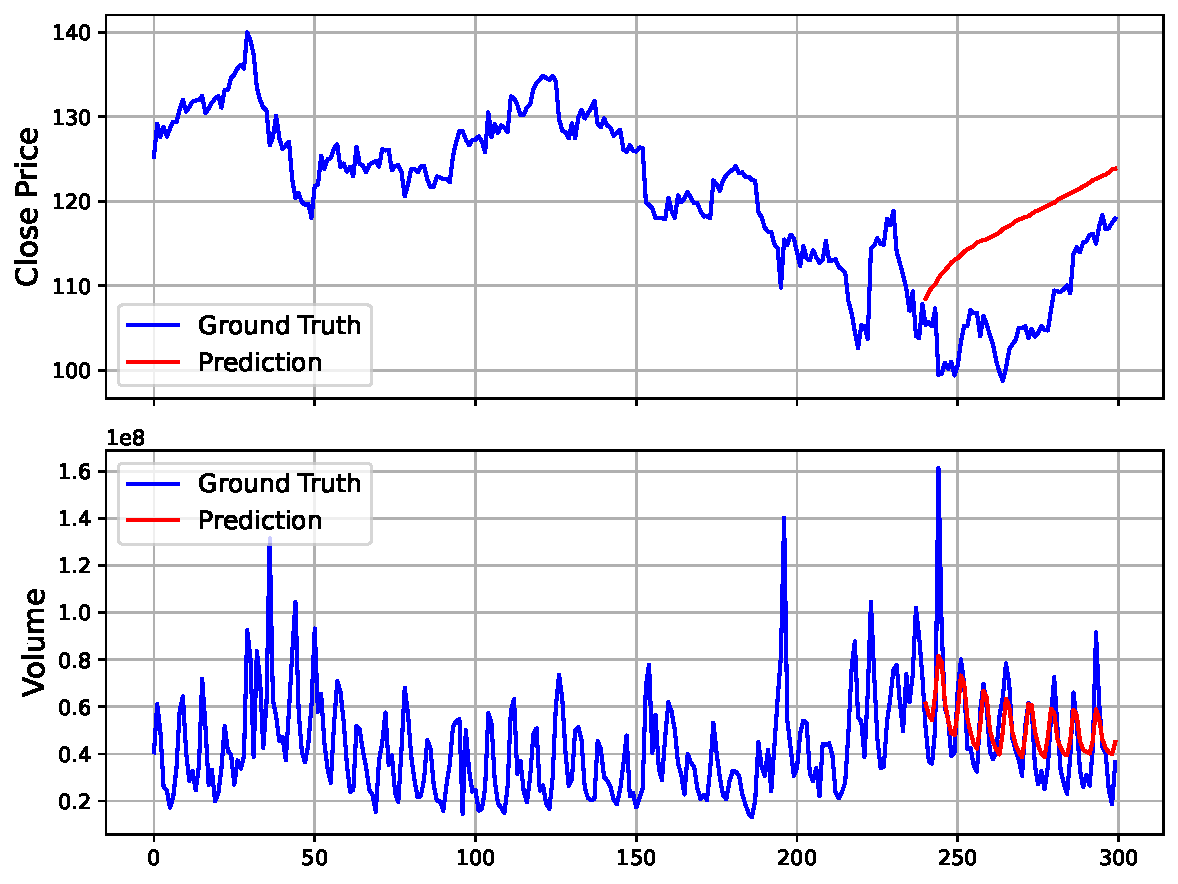
\includegraphics[width=\linewidth]{pred_imgs/pred_visualize_stock_XNAS_NVDA_60min_TimeMOE_small.pdf}
        \caption{$\text{TimeMOE}_{small}$}
    \end{subfigure}
    \hfill
    \begin{subfigure}[b]{0.33\textwidth}
        \centering
        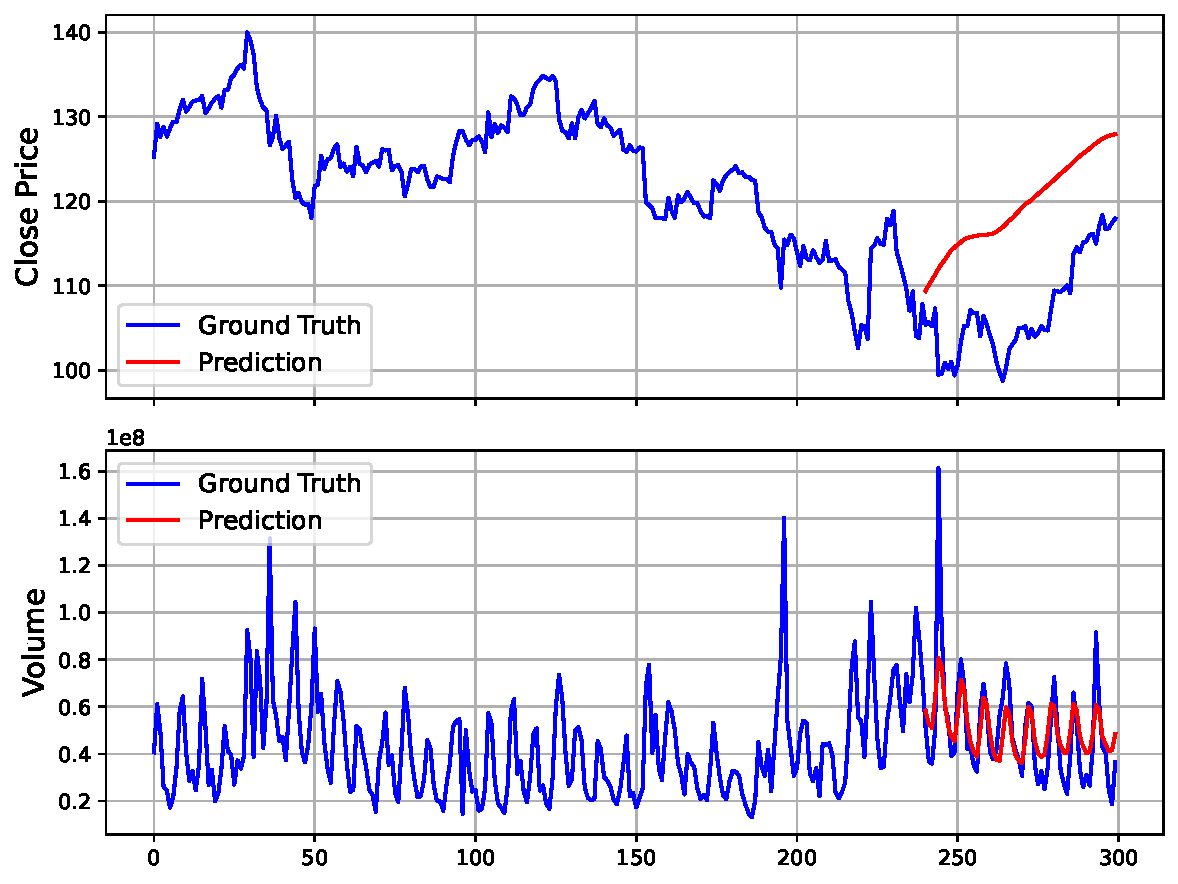
\includegraphics[width=\linewidth]{pred_imgs/pred_visualize_stock_XNAS_NVDA_60min_TimeMOE_large.pdf}
        \caption{$\text{TimeMOE}_{large}$}
    \end{subfigure}
    \hfill
    \begin{subfigure}[b]{0.33\textwidth}
        \centering
        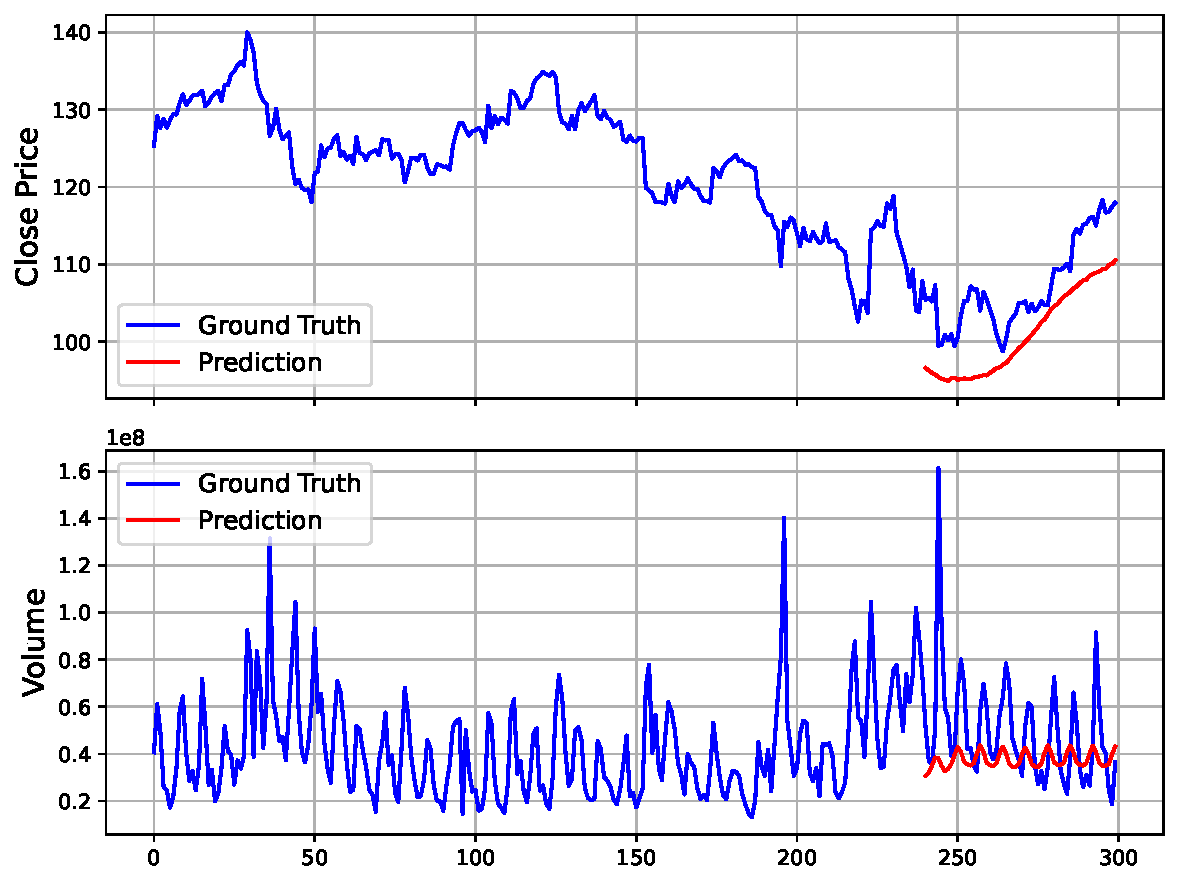
\includegraphics[width=\linewidth]{pred_imgs/pred_visualize_stock_XNAS_NVDA_60min_TimesFM.pdf}
        \caption{TimesFM}
    \end{subfigure}

    \vspace{0.1cm}

    \begin{subfigure}[b]{0.33\textwidth}
        \centering
        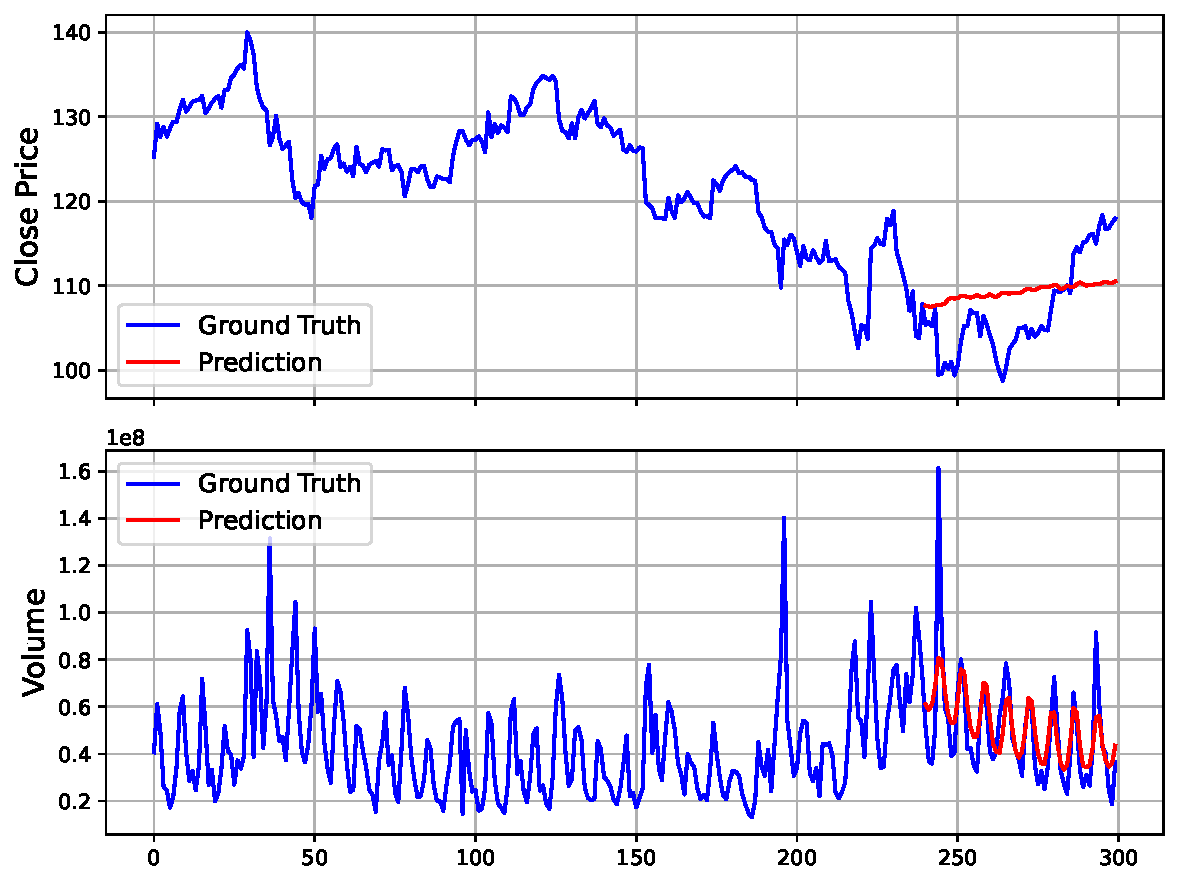
\includegraphics[width=\linewidth]{pred_imgs/pred_visualize_stock_XNAS_NVDA_60min_Chronos_small.pdf}
        \caption{$\text{Chronos}_{small}$}
    \end{subfigure}
    \hfill
    \begin{subfigure}[b]{0.33\textwidth}
        \centering
        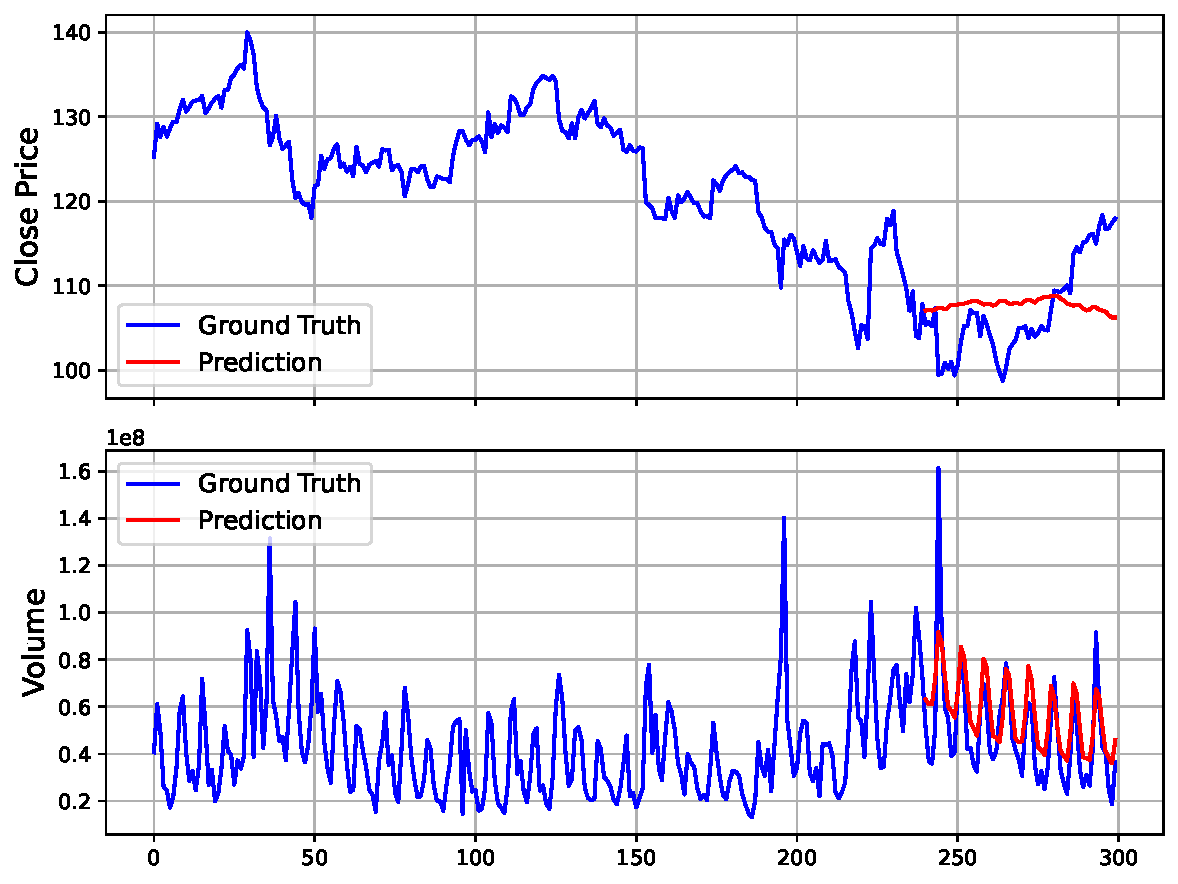
\includegraphics[width=\linewidth]{pred_imgs/pred_visualize_stock_XNAS_NVDA_60min_Chronos_base.pdf}
        \caption{$\text{Chronos}_{base}$}
    \end{subfigure}
    \hfill
    \begin{subfigure}[b]{0.33\textwidth}
        \centering
        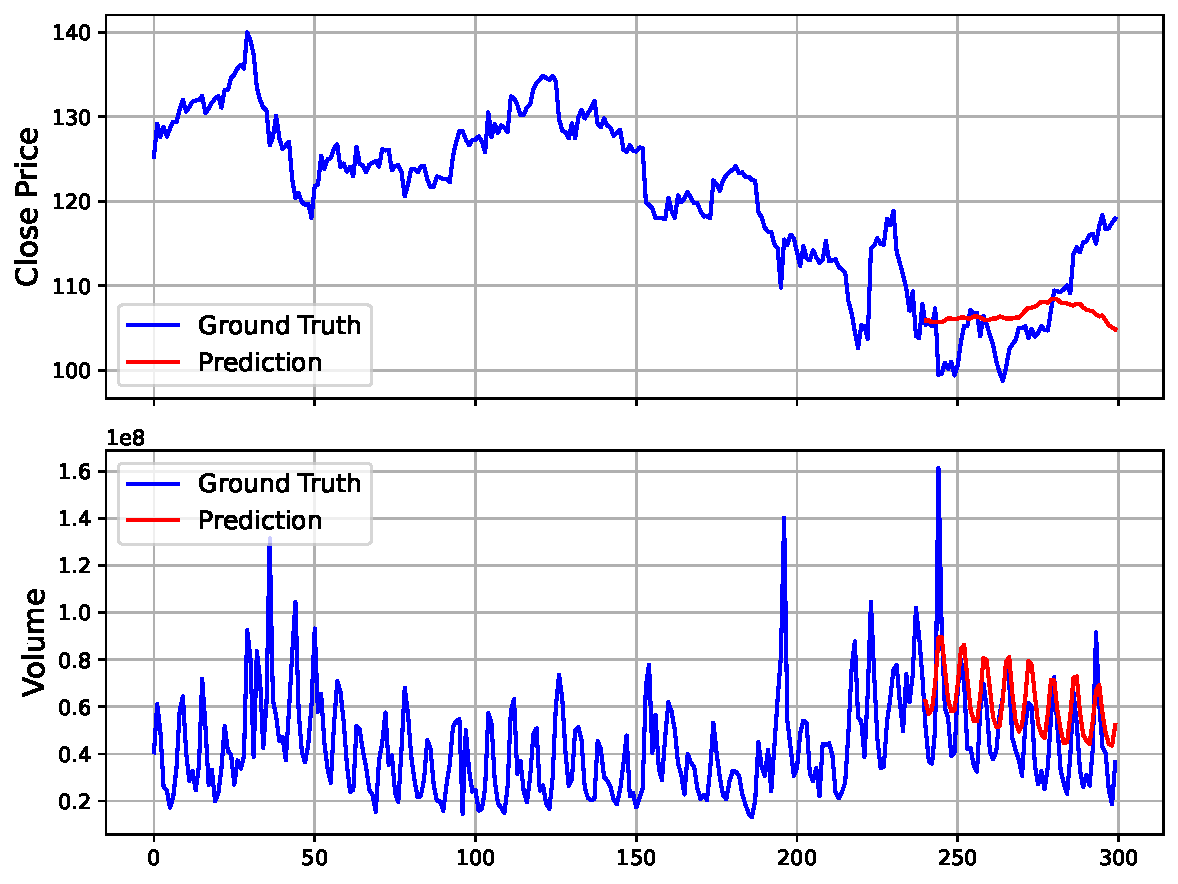
\includegraphics[width=\linewidth]{pred_imgs/pred_visualize_stock_XNAS_NVDA_60min_Chronos_large.pdf}
        \caption{$\text{Chronos}_{large}$}
    \end{subfigure}

    \vspace{0.1cm}

    \begin{subfigure}[b]{0.33\textwidth}
        \centering
        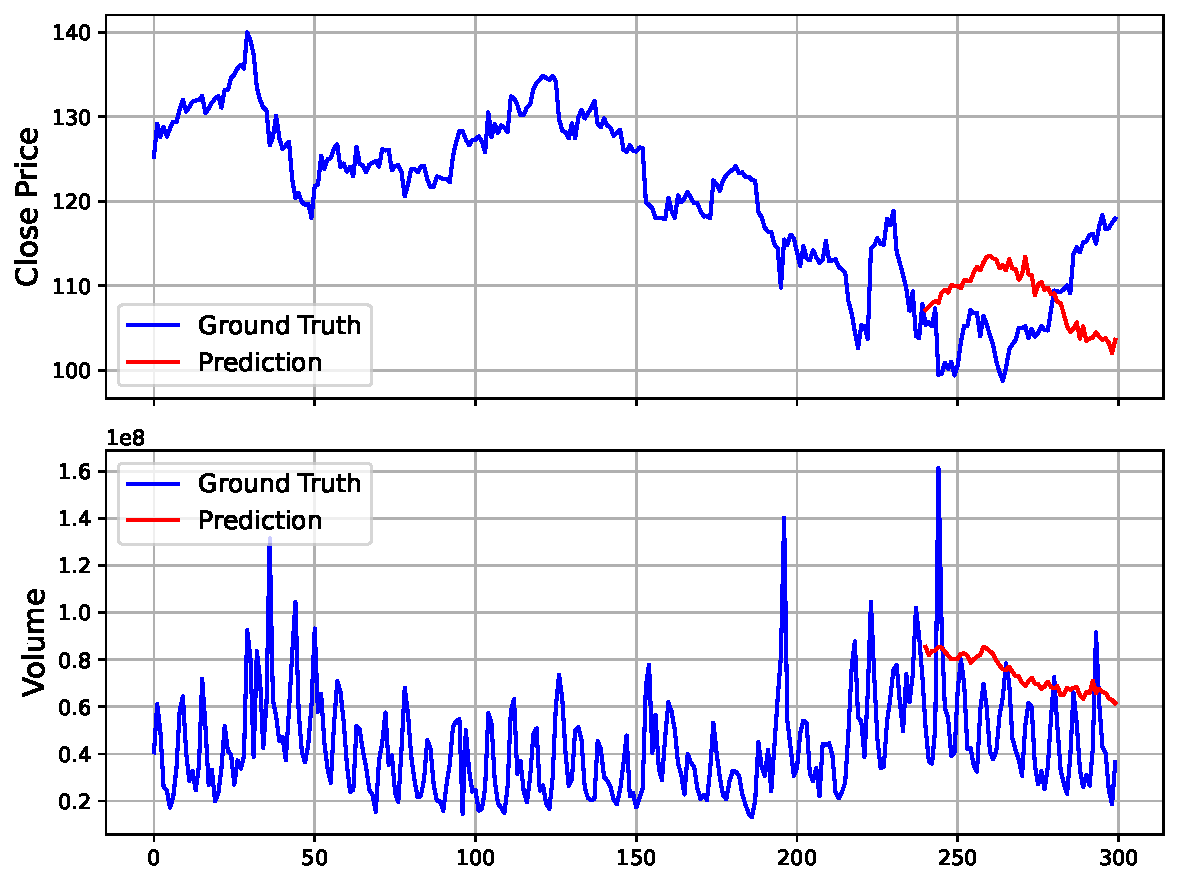
\includegraphics[width=\linewidth]{pred_imgs/pred_visualize_stock_XNAS_NVDA_60min_iTransformer.pdf}
        \caption{iTransformer}
    \end{subfigure}
    \hfill
    \begin{subfigure}[b]{0.33\textwidth}
        \centering
        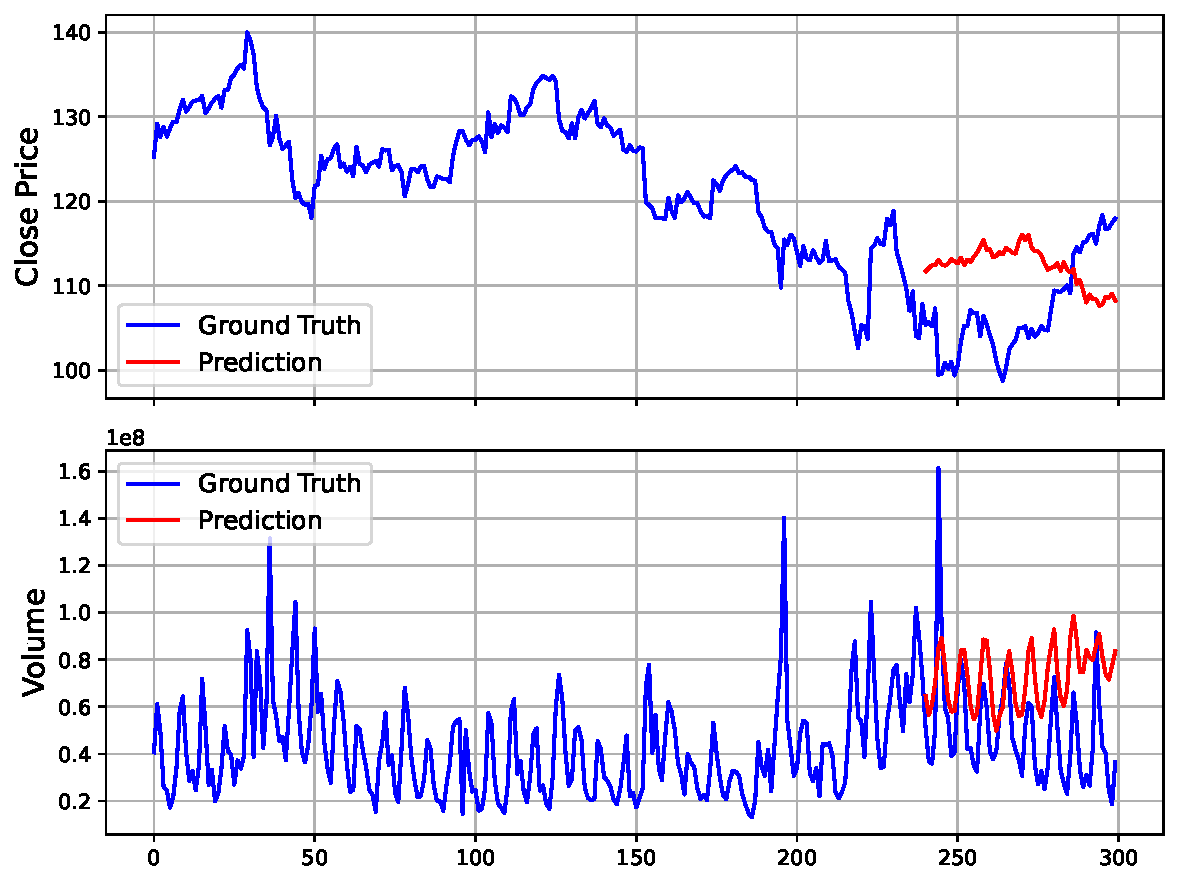
\includegraphics[width=\linewidth]{pred_imgs/pred_visualize_stock_XNAS_NVDA_60min_DLinear.pdf}
        \caption{DLinear}
    \end{subfigure}
    \hfill
    \begin{subfigure}[b]{0.33\textwidth}
        \centering
        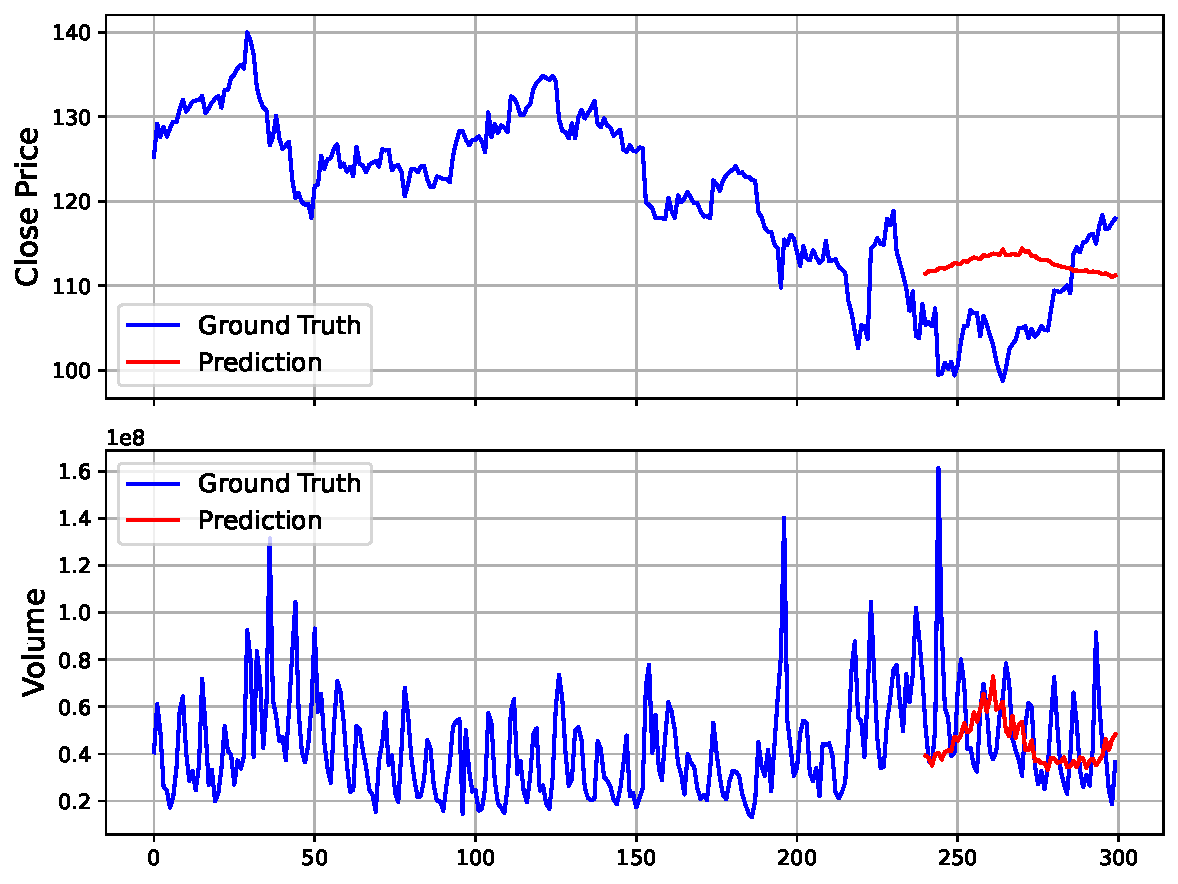
\includegraphics[width=\linewidth]{pred_imgs/pred_visualize_stock_XNAS_NVDA_60min_TimesNet.pdf}
        \caption{TimesNet}
    \end{subfigure}

    \caption{1시간 K-line 데이터를 기반으로 한 NVIDIA (NASDAQ: NVDA)의 `Close Price'와 `Volume' 예측 결과. 모델은 240스텝 look-back 윈도우를 사용하여 60스텝 horizon을 예측한다. \textcolor{blue}{Blue} 선은 정답값을 나타내고 \textcolor{red}{red} 선은 모델의 예측값을 나타낸다.}
    \label{fig:pred_case_3}
\end{figure*}


\begin{figure*}[ht]
    \centering

    \begin{subfigure}[b]{0.33\textwidth}
        \centering
        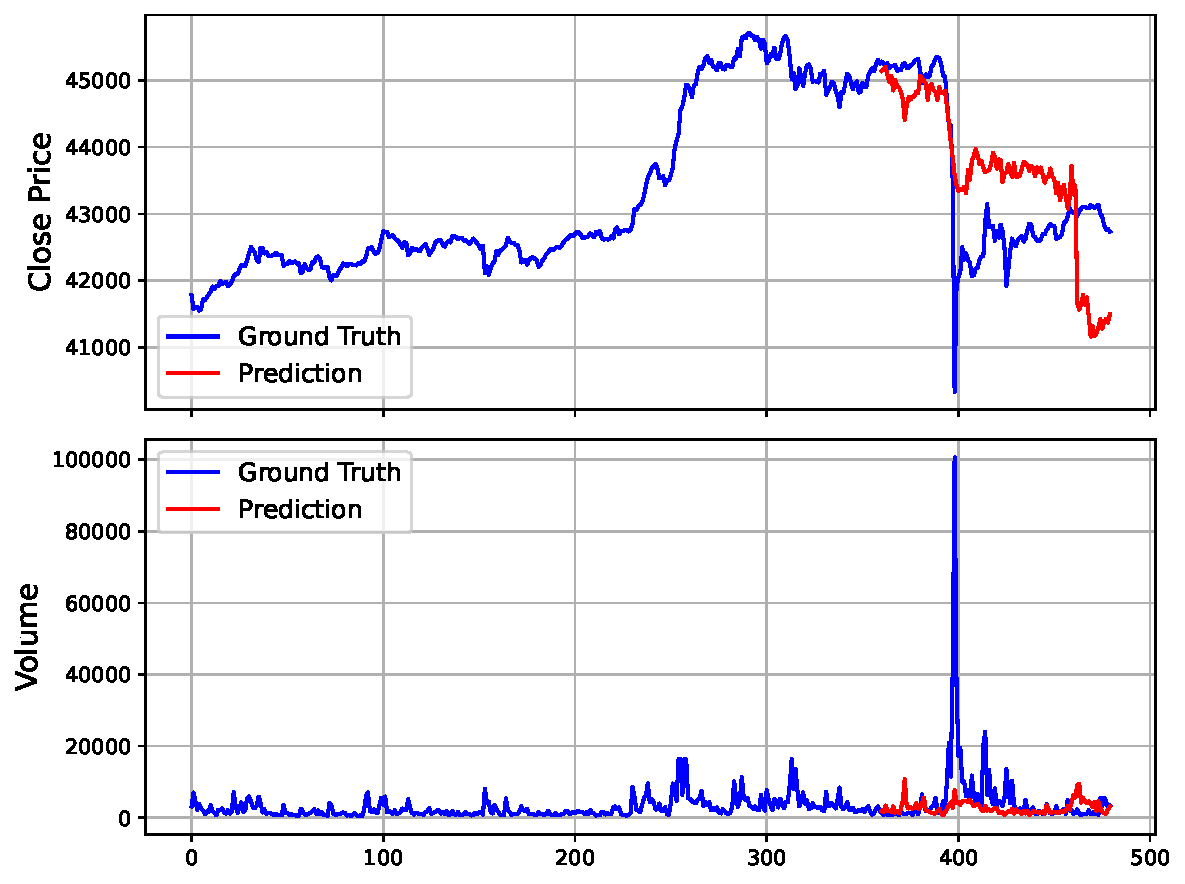
\includegraphics[width=\linewidth]{pred_imgs/pred_visualize_crypto_BTCUSDT_15min_Kronos_small.pdf}
        \caption{$\text{Kronos}_{small}$}
    \end{subfigure}
    \hfill
    \begin{subfigure}[b]{0.33\textwidth}
        \centering
        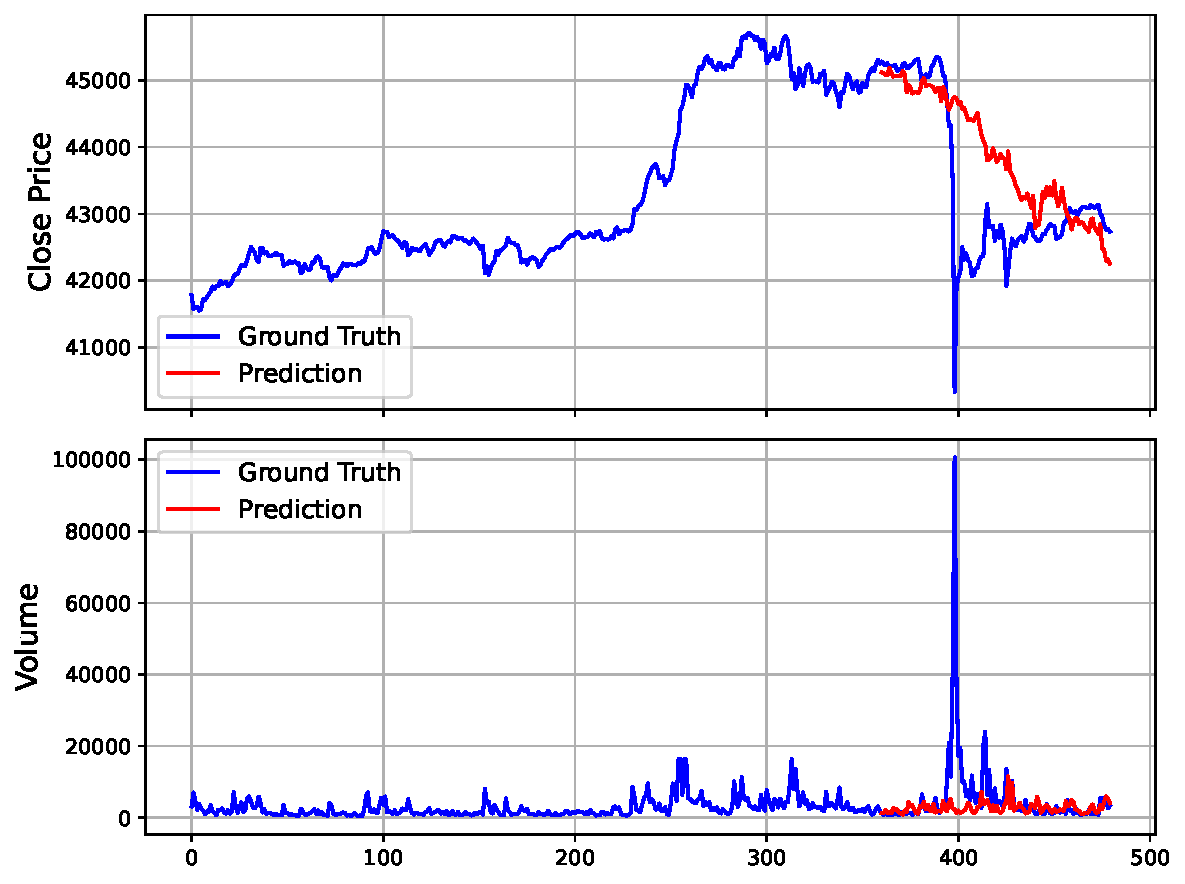
\includegraphics[width=\linewidth]{pred_imgs/pred_visualize_crypto_BTCUSDT_15min_Kronos_base.pdf}
        \caption{$\text{Kronos}_{base}$}
    \end{subfigure}
    \hfill
    \begin{subfigure}[b]{0.33\textwidth}
        \centering
        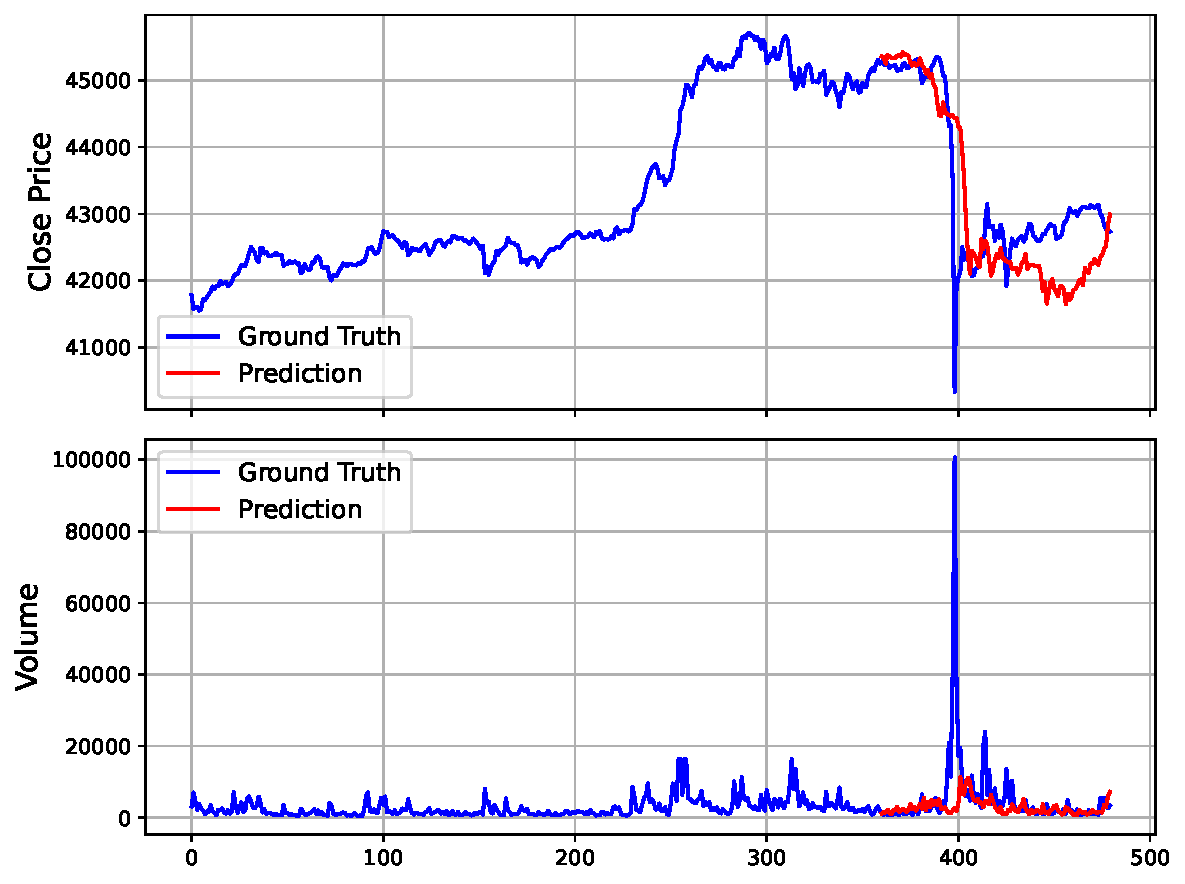
\includegraphics[width=\linewidth]{pred_imgs/pred_visualize_crypto_BTCUSDT_15min_Kronos_large.pdf}
        \caption{$\text{Kronos}_{large}$}
    \end{subfigure}

    \vspace{0.1cm}

    \begin{subfigure}[b]{0.33\textwidth}
        \centering
        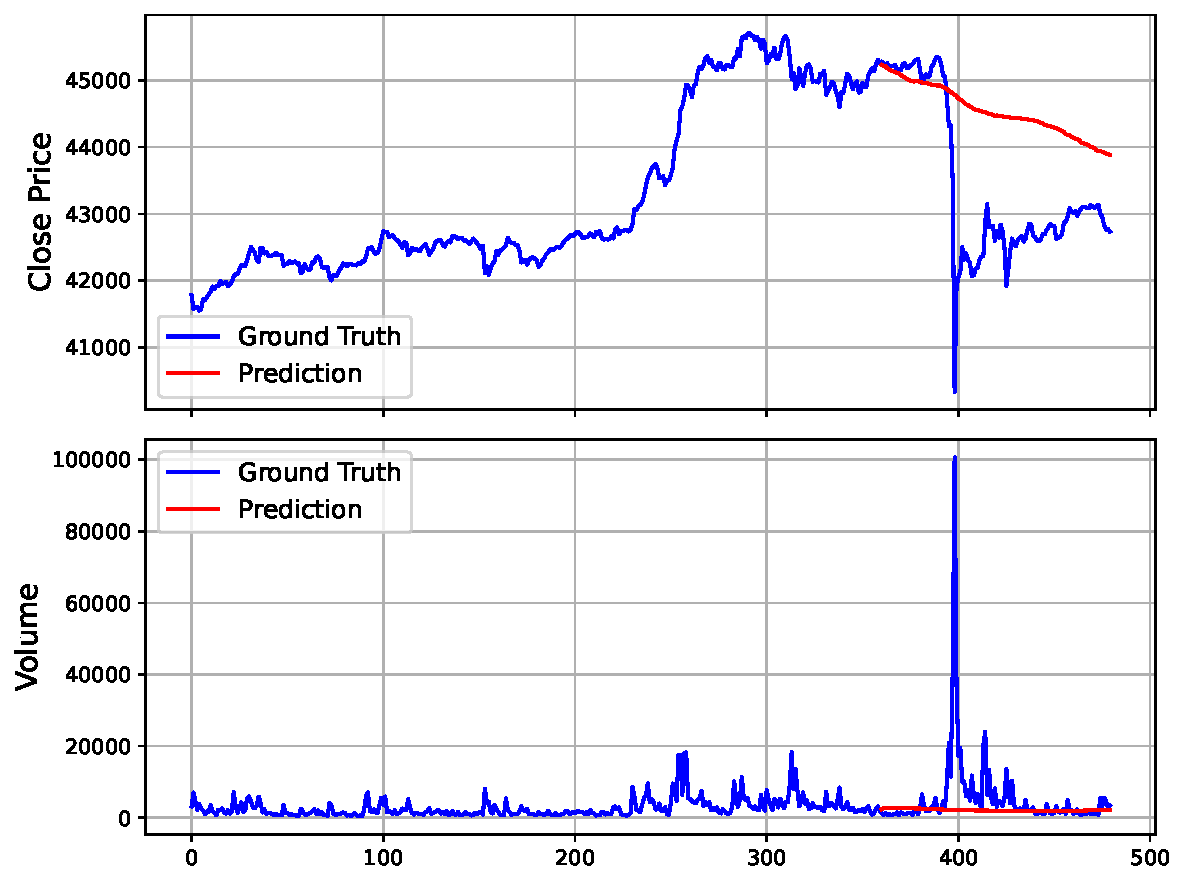
\includegraphics[width=\linewidth]{pred_imgs/pred_visualize_crypto_BTCUSDT_15min_TimeMOE_small.pdf}
        \caption{$\text{TimeMOE}_{small}$}
    \end{subfigure}
    \hfill
    \begin{subfigure}[b]{0.33\textwidth}
        \centering
        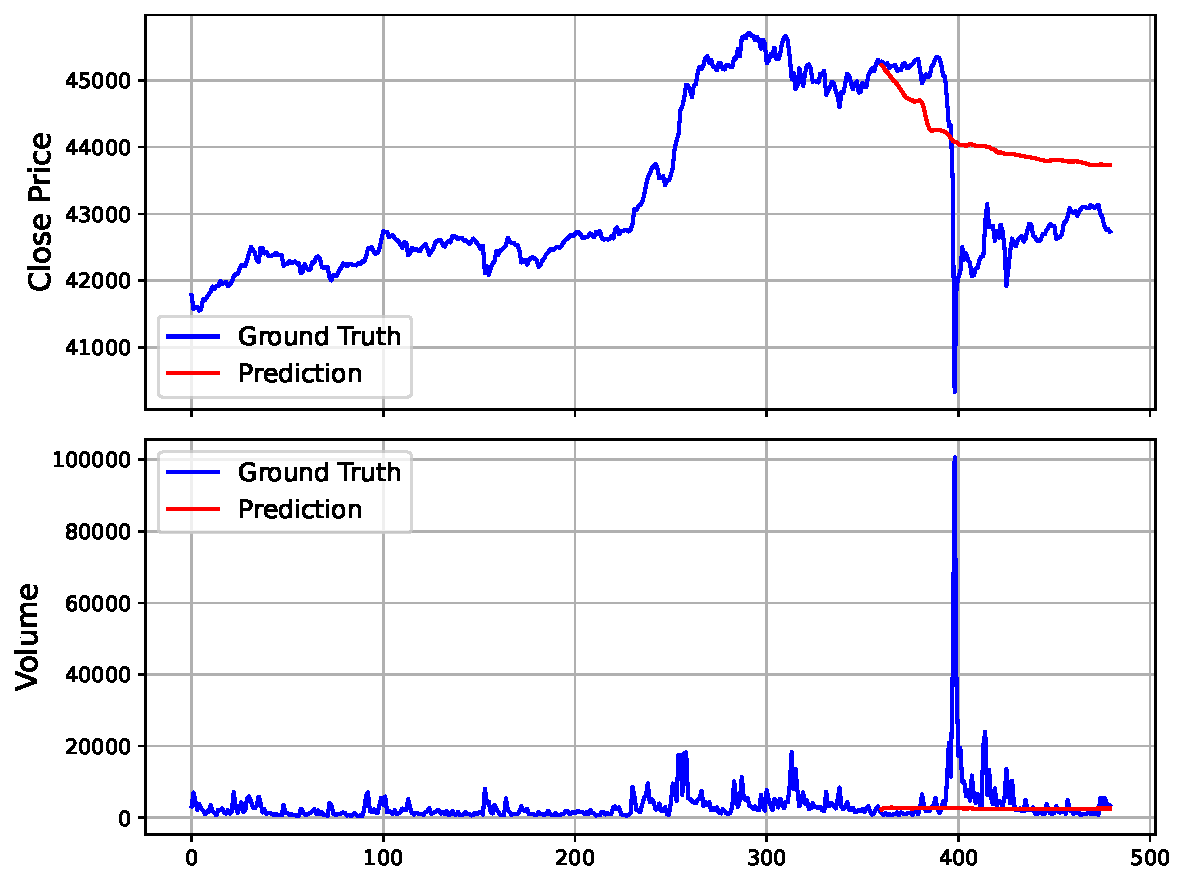
\includegraphics[width=\linewidth]{pred_imgs/pred_visualize_crypto_BTCUSDT_15min_TimeMOE_large.pdf}
        \caption{$\text{TimeMOE}_{large}$}
    \end{subfigure}
    \hfill
    \begin{subfigure}[b]{0.33\textwidth}
        \centering
        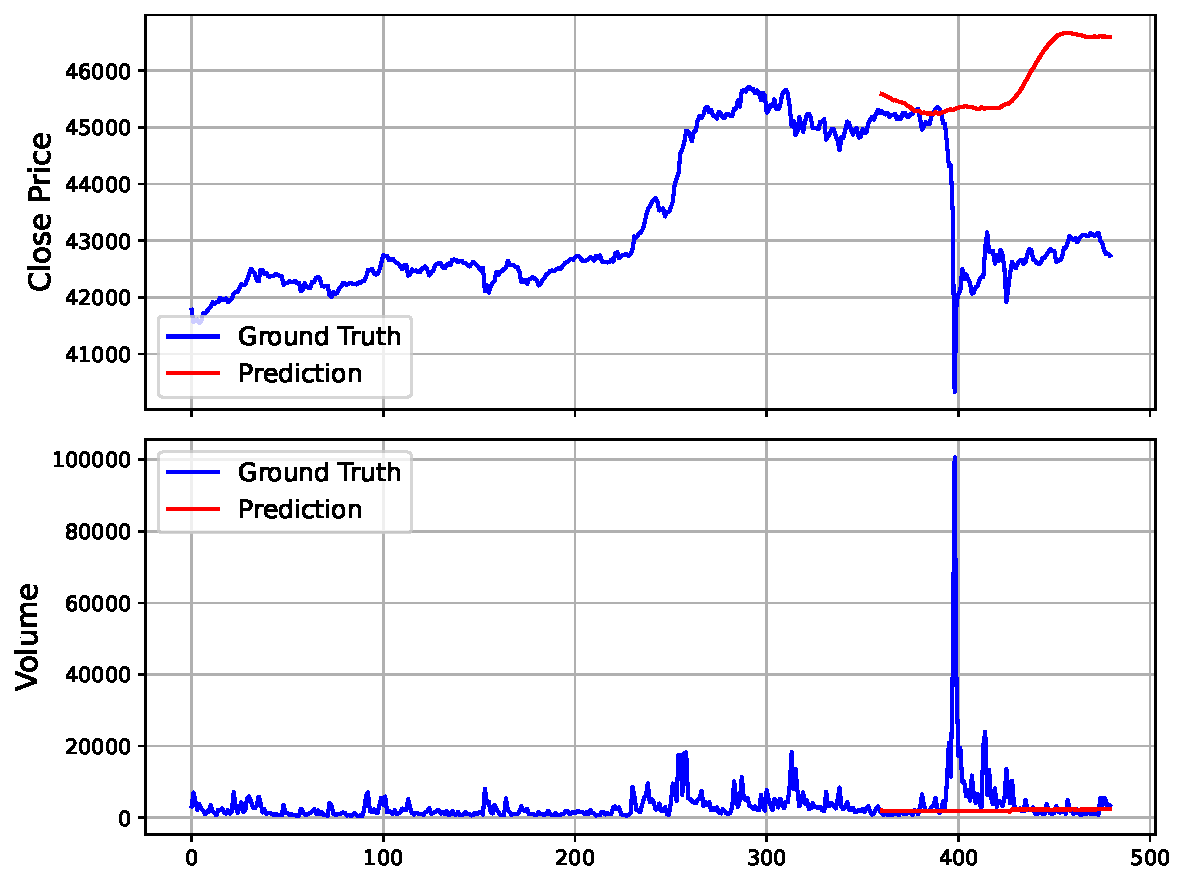
\includegraphics[width=\linewidth]{pred_imgs/pred_visualize_crypto_BTCUSDT_15min_TimesFM.pdf}
        \caption{TimesFM}
    \end{subfigure}

    \vspace{0.1cm}

    \begin{subfigure}[b]{0.33\textwidth}
        \centering
        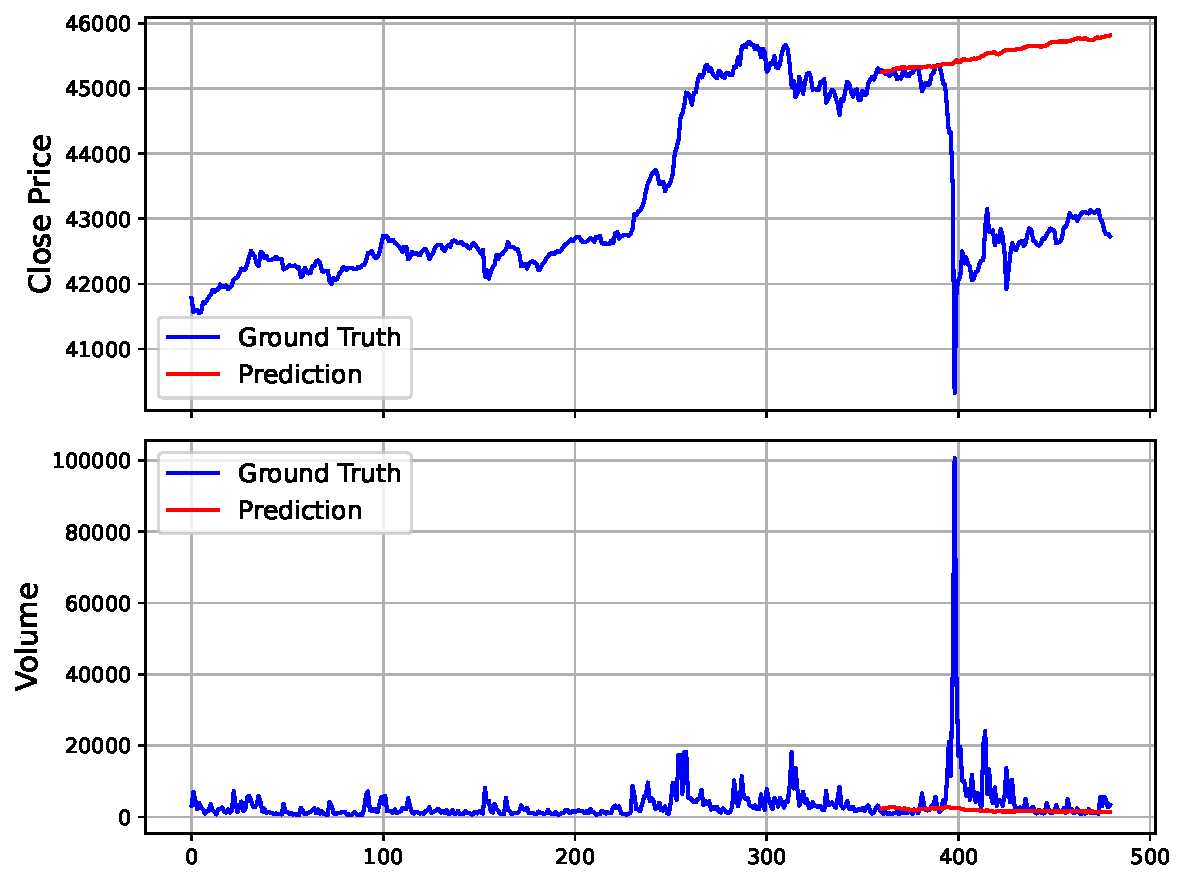
\includegraphics[width=\linewidth]{pred_imgs/pred_visualize_crypto_BTCUSDT_15min_Chronos_small.pdf}
        \caption{$\text{Chronos}_{small}$}
    \end{subfigure}
    \hfill
    \begin{subfigure}[b]{0.33\textwidth}
        \centering
        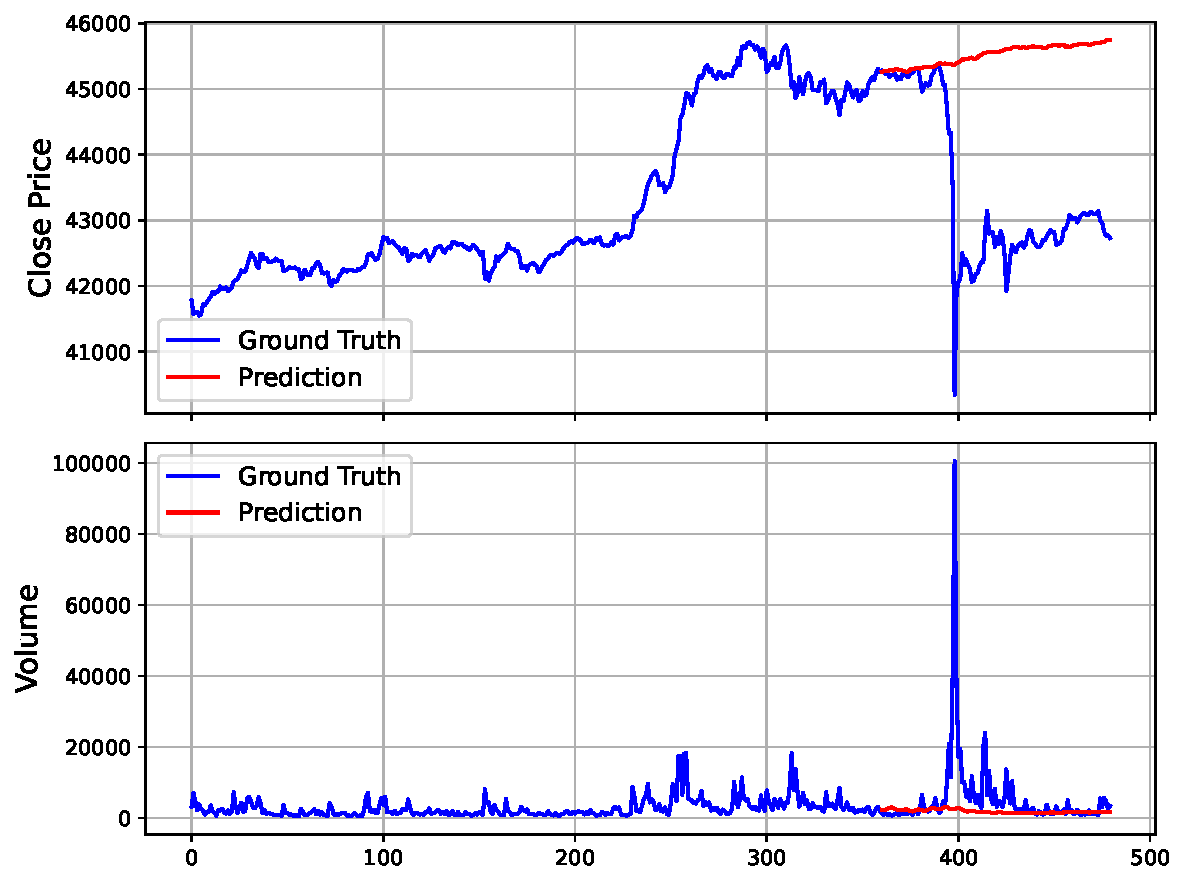
\includegraphics[width=\linewidth]{pred_imgs/pred_visualize_crypto_BTCUSDT_15min_Chronos_base.pdf}
        \caption{$\text{Chronos}_{base}$}
    \end{subfigure}
    \hfill
    \begin{subfigure}[b]{0.33\textwidth}
        \centering
        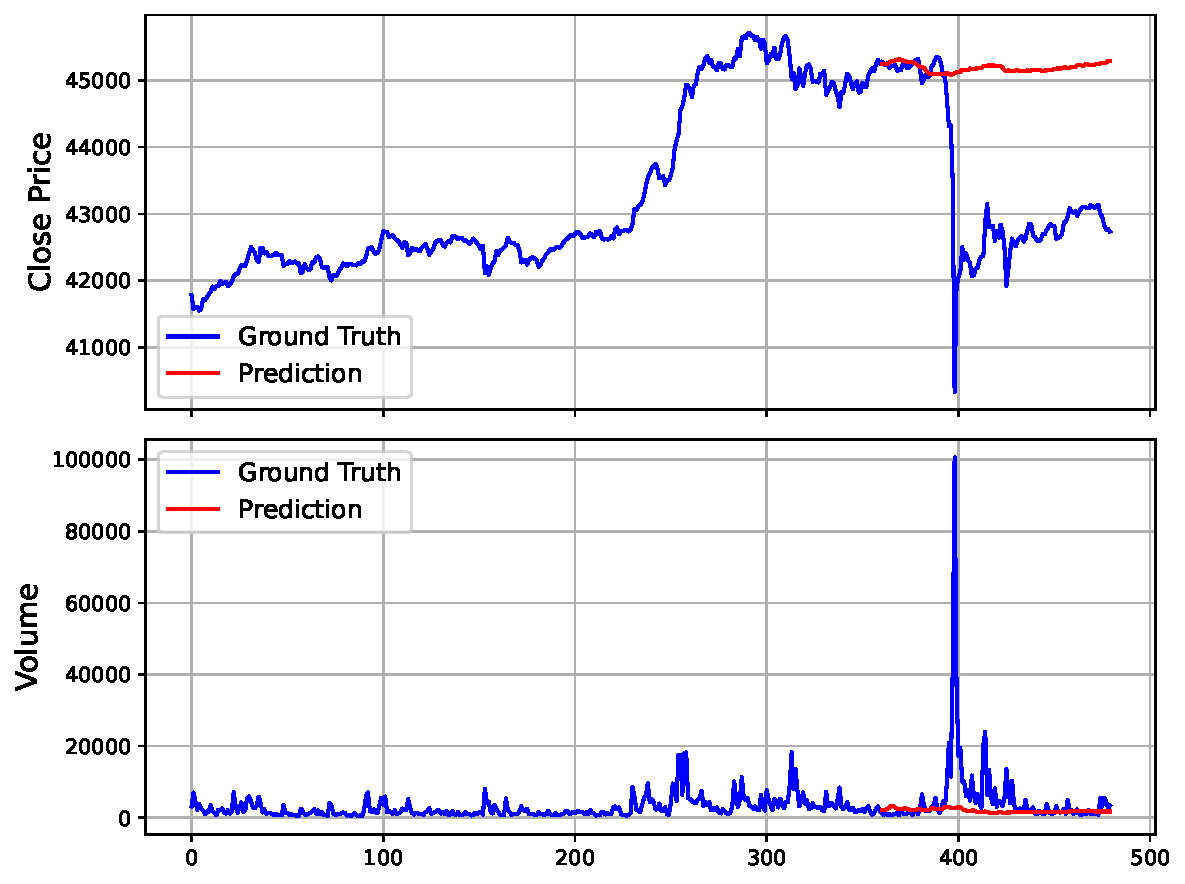
\includegraphics[width=\linewidth]{pred_imgs/pred_visualize_crypto_BTCUSDT_15min_Chronos_large.pdf}
        \caption{$\text{Chronos}_{large}$}
    \end{subfigure}

    \vspace{0.1cm}

    \begin{subfigure}[b]{0.33\textwidth}
        \centering
        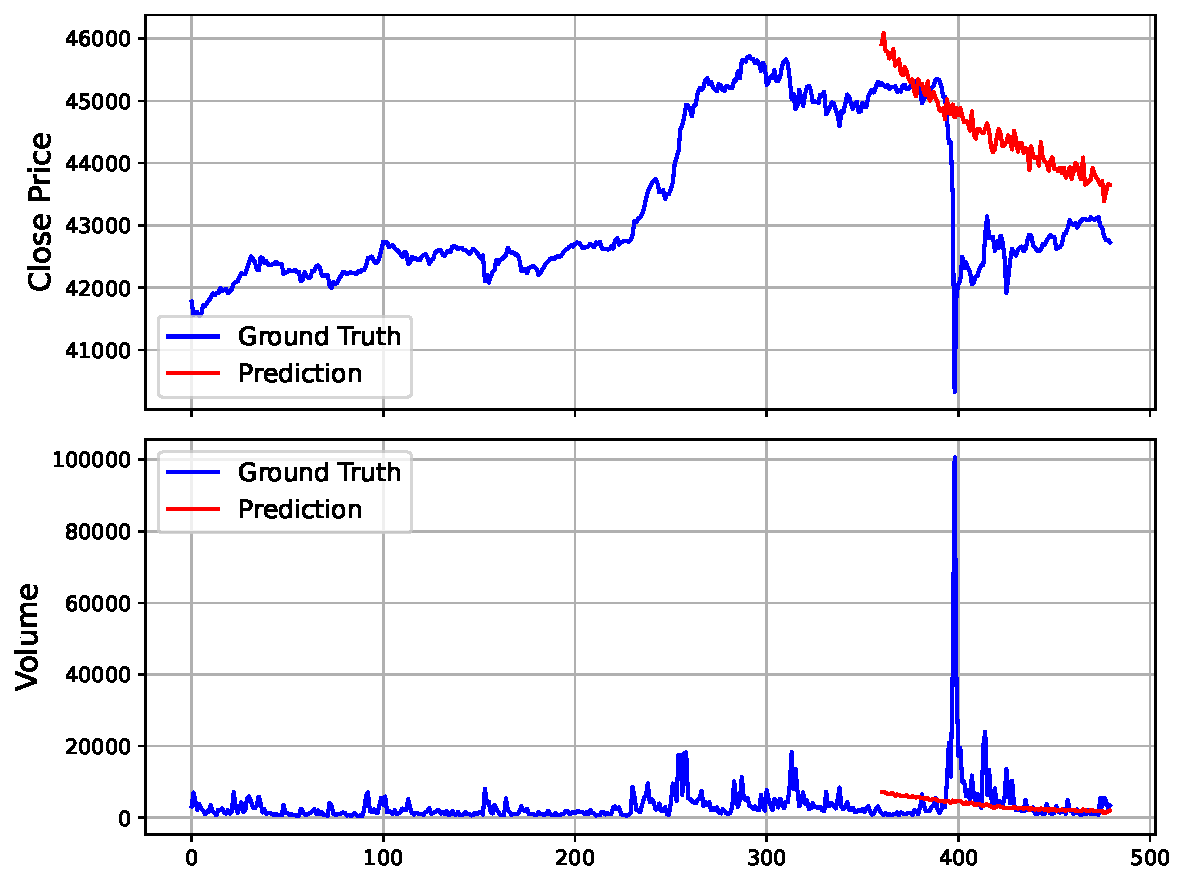
\includegraphics[width=\linewidth]{pred_imgs/pred_visualize_crypto_BTCUSDT_15min_iTransformer.pdf}
        \caption{iTransformer}
    \end{subfigure}
    \hfill
    \begin{subfigure}[b]{0.33\textwidth}
        \centering
        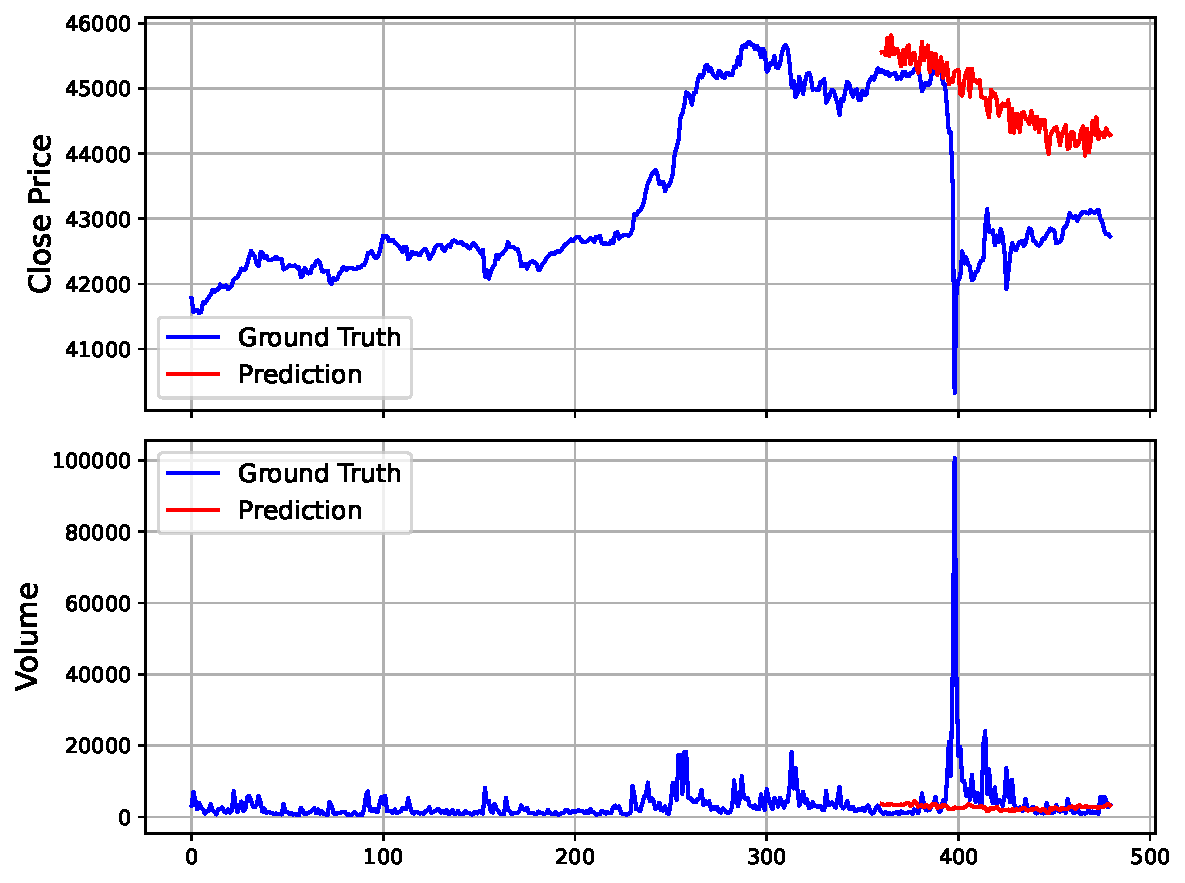
\includegraphics[width=\linewidth]{pred_imgs/pred_visualize_crypto_BTCUSDT_15min_DLinear.pdf}
        \caption{DLinear}
    \end{subfigure}
    \hfill
    \begin{subfigure}[b]{0.33\textwidth}
        \centering
        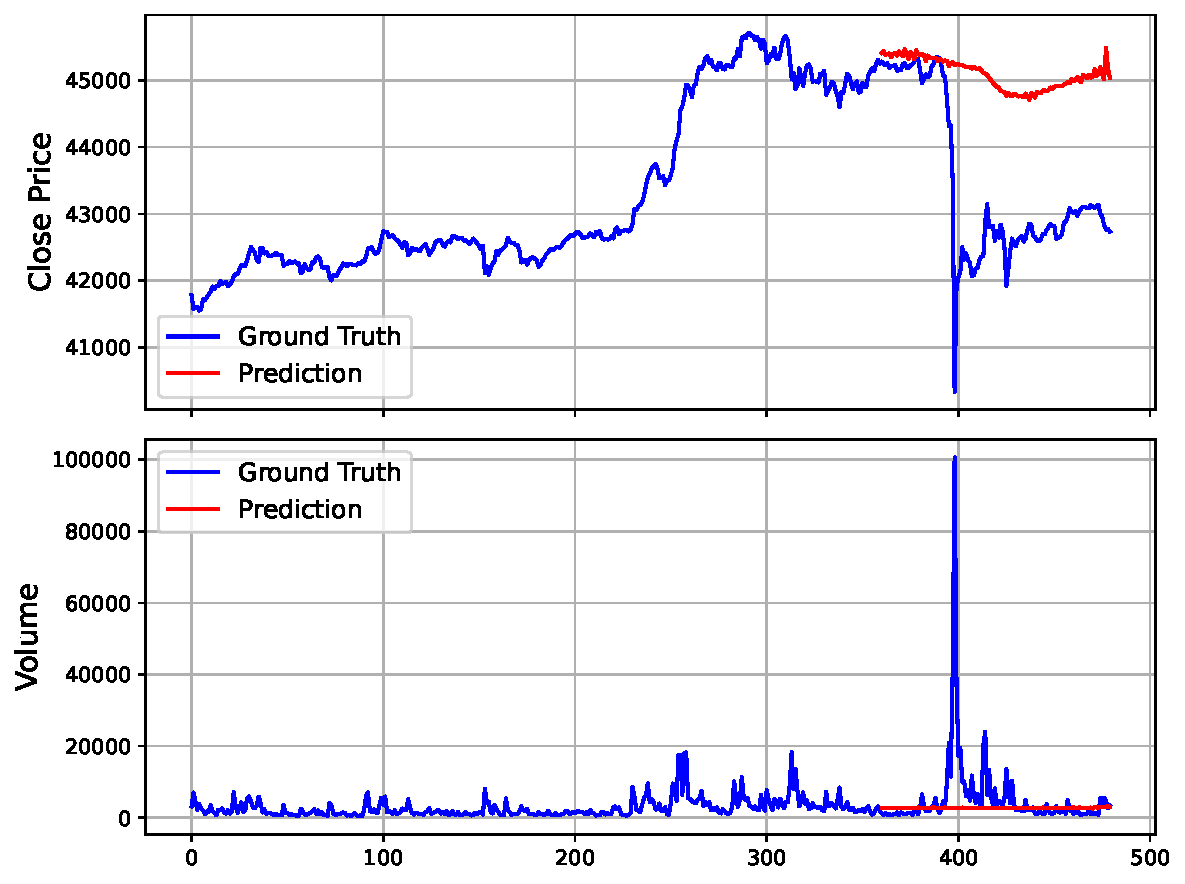
\includegraphics[width=\linewidth]{pred_imgs/pred_visualize_crypto_BTCUSDT_15min_TimesNet.pdf}
        \caption{TimesNet}
    \end{subfigure}

    \caption{15분 K-line 데이터를 기반으로 한 Binance의 BTC/USDT 무기한 계약의 `Close Price'와 `Volume' 예측 결과. 모델은 360스텝 look-back 윈도우를 사용하여 120스텝 horizon을 예측한다. \textcolor{blue}{Blue} 선은 정답값을 나타내고 \textcolor{red}{red} 선은 모델의 예측값을 나타낸다.}
    \label{fig:pred_case_4}
\end{figure*}

\begin{figure*}[ht]
    \centering

    \begin{subfigure}[b]{0.33\textwidth}
        \centering
        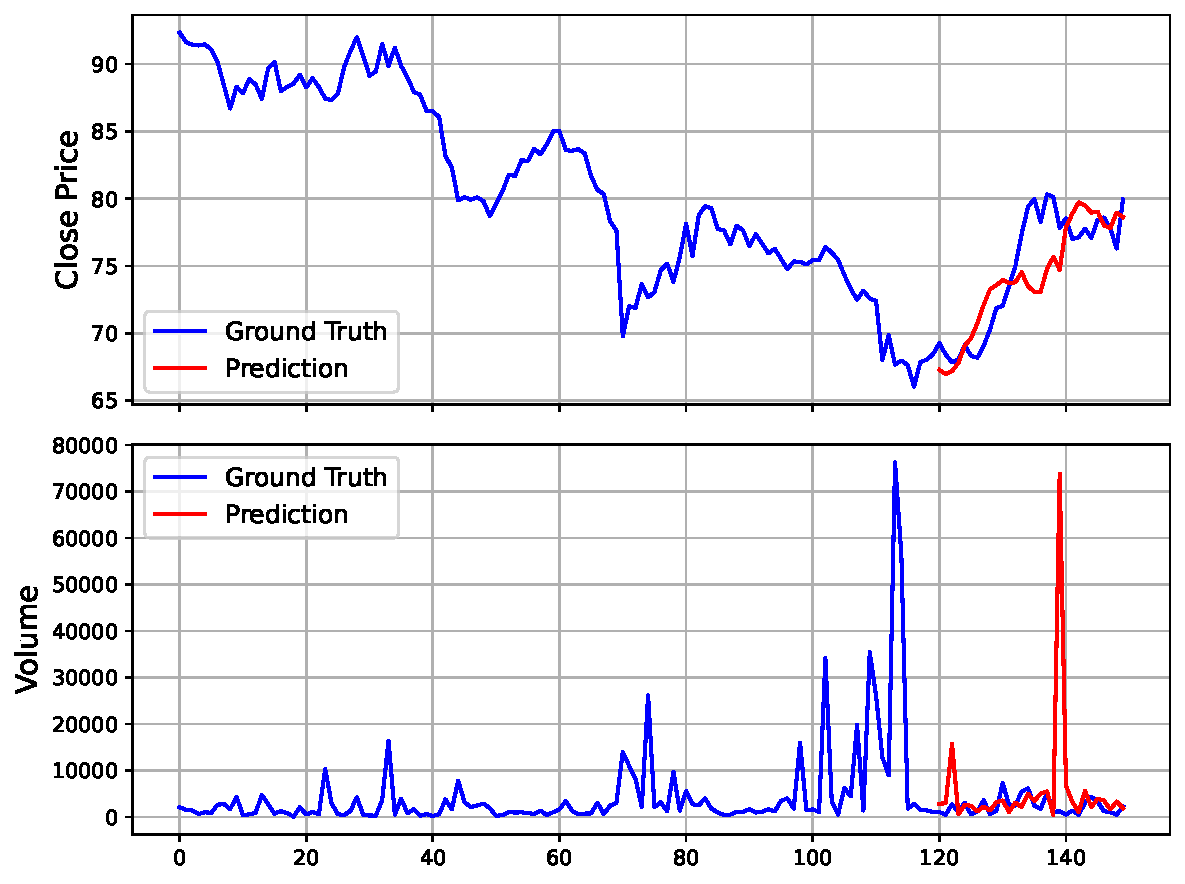
\includegraphics[width=\linewidth]{pred_imgs/pred_visualize_stock_XFRA_BMW_daily_Kronos_small.pdf}
        \caption{$\text{Kronos}_{small}$}
    \end{subfigure}
    \hfill
    \begin{subfigure}[b]{0.33\textwidth}
        \centering
        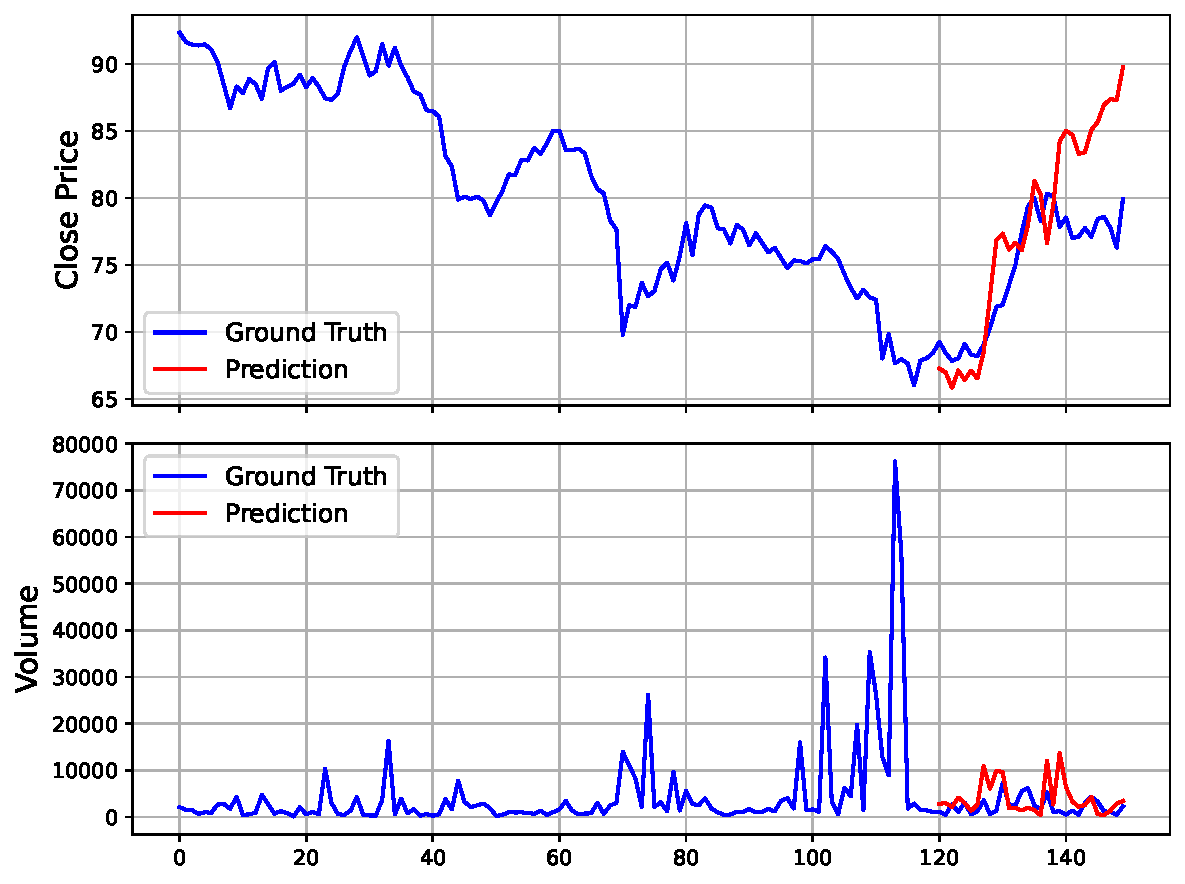
\includegraphics[width=\linewidth]{pred_imgs/pred_visualize_stock_XFRA_BMW_daily_Kronos_base.pdf}
        \caption{$\text{Kronos}_{base}$}
    \end{subfigure}
    \hfill
    \begin{subfigure}[b]{0.33\textwidth}
        \centering
        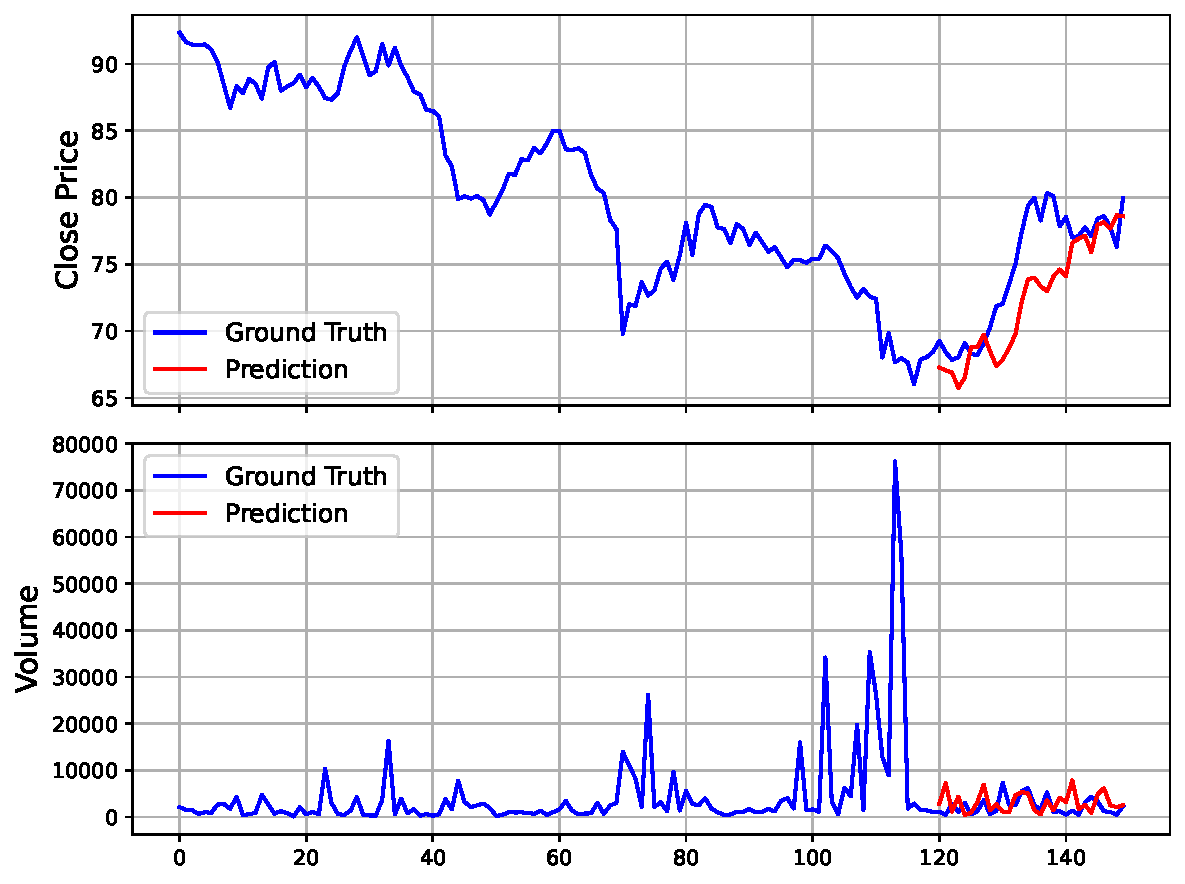
\includegraphics[width=\linewidth]{pred_imgs/pred_visualize_stock_XFRA_BMW_daily_Kronos_large.pdf}
        \caption{$\text{Kronos}_{large}$}
    \end{subfigure}

    \vspace{0.1cm}

    \begin{subfigure}[b]{0.33\textwidth}
        \centering
        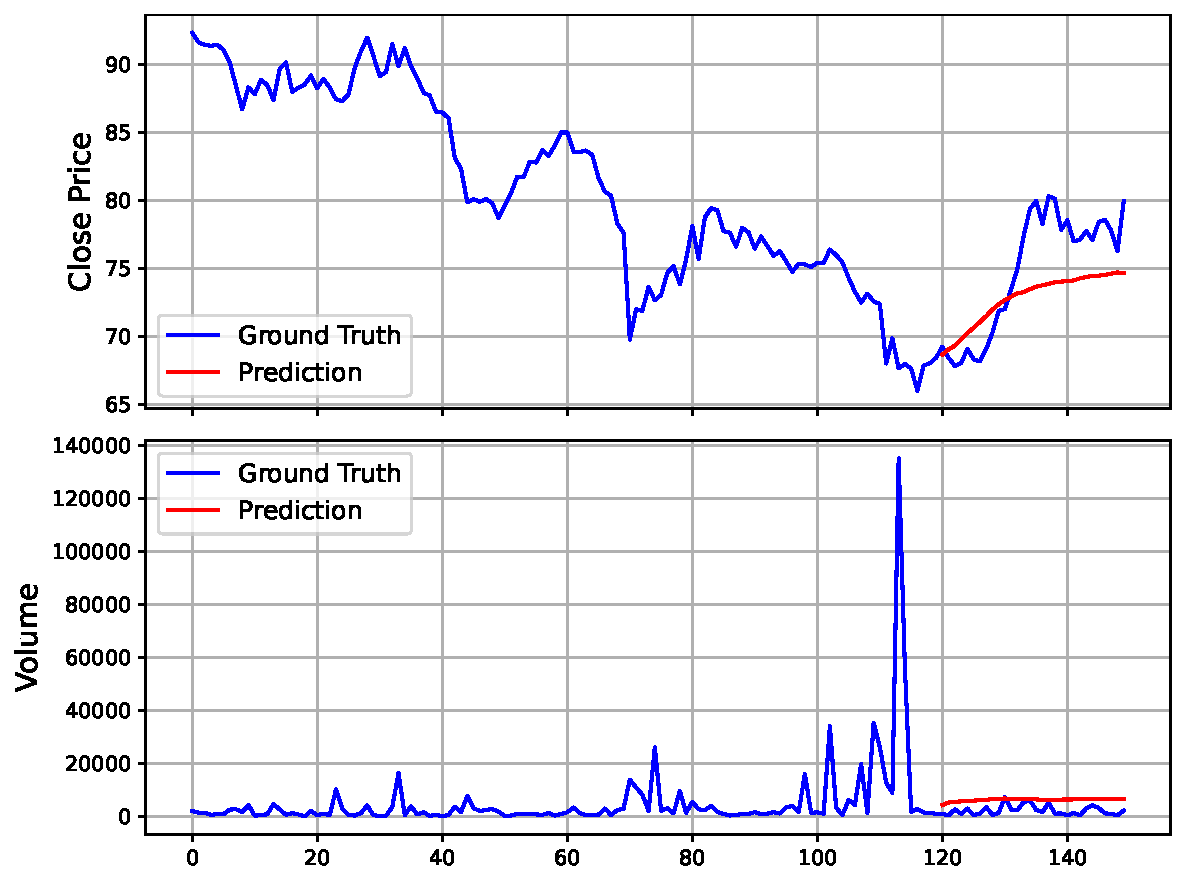
\includegraphics[width=\linewidth]{pred_imgs/pred_visualize_stock_XFRA_BMW_daily_TimeMOE_small.pdf}
        \caption{$\text{TimeMOE}_{small}$}
    \end{subfigure}
    \hfill
    \begin{subfigure}[b]{0.33\textwidth}
        \centering
        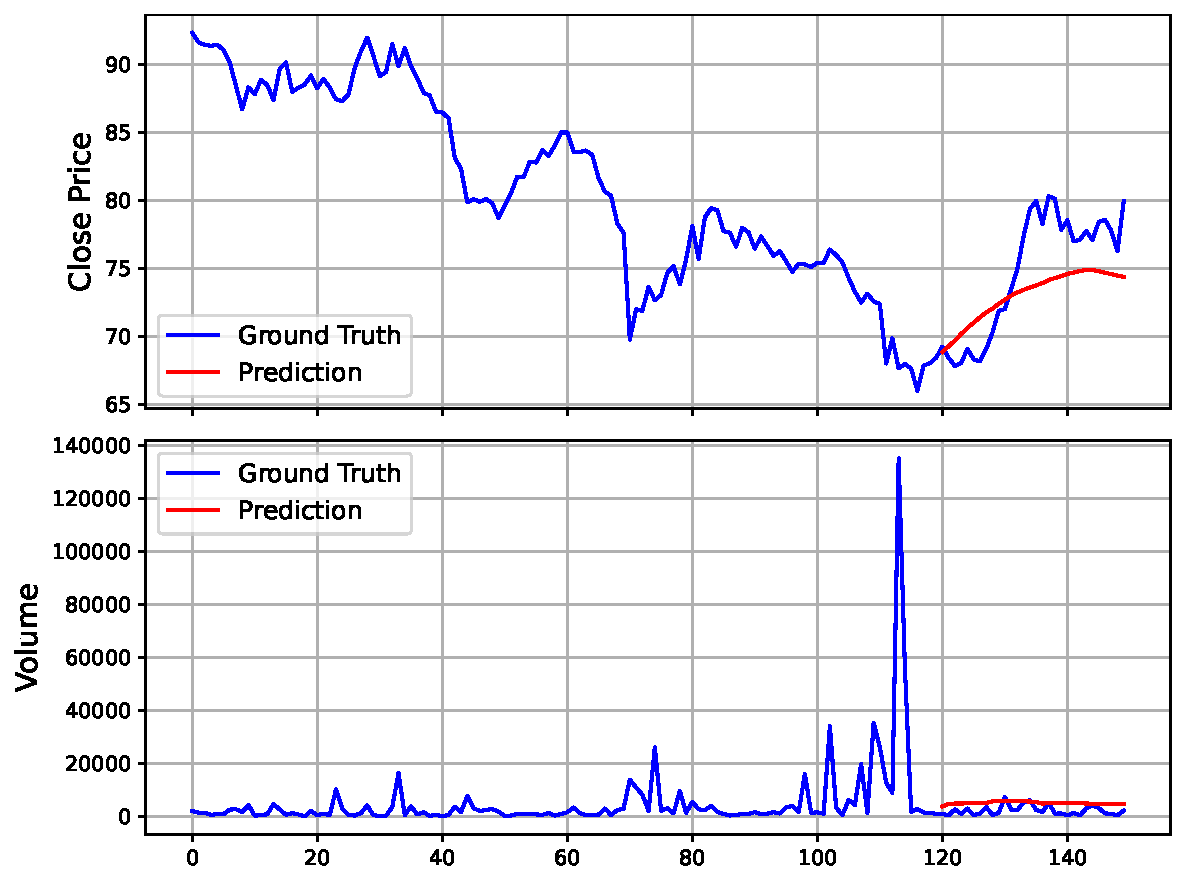
\includegraphics[width=\linewidth]{pred_imgs/pred_visualize_stock_XFRA_BMW_daily_TimeMOE_large.pdf}
        \caption{$\text{TimeMOE}_{large}$}
    \end{subfigure}
    \hfill
    \begin{subfigure}[b]{0.33\textwidth}
        \centering
        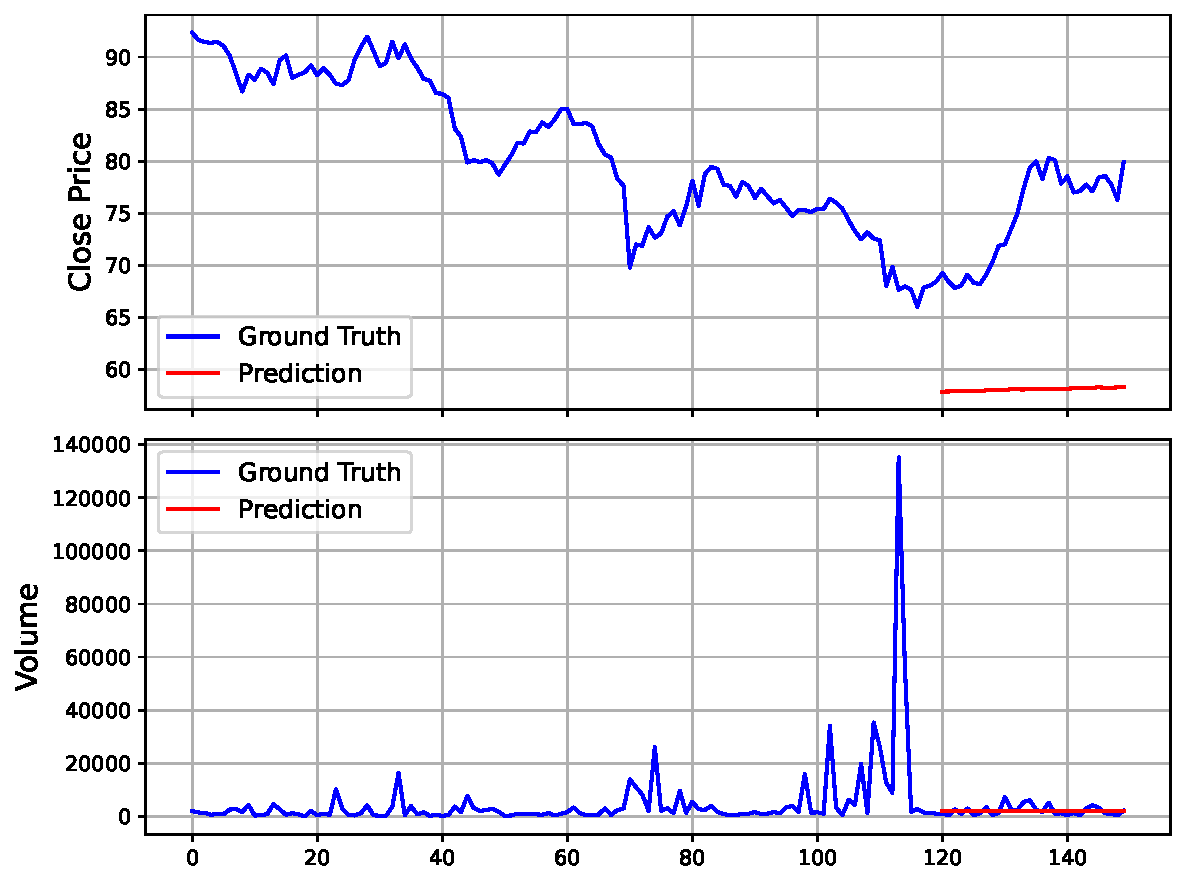
\includegraphics[width=\linewidth]{pred_imgs/pred_visualize_stock_XFRA_BMW_daily_TimesFM.pdf}
        \caption{TimesFM}
    \end{subfigure}

    \vspace{0.1cm}

    \begin{subfigure}[b]{0.33\textwidth}
        \centering
        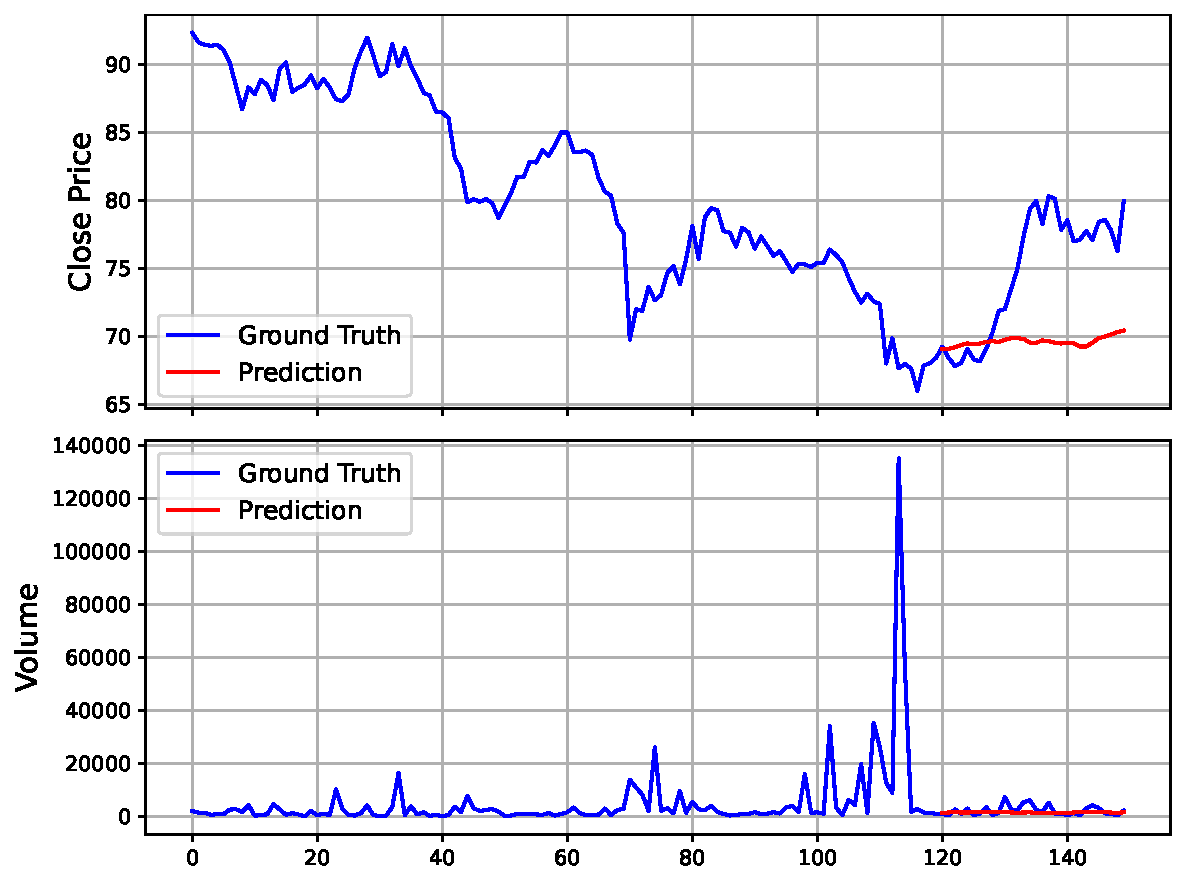
\includegraphics[width=\linewidth]{pred_imgs/pred_visualize_stock_XFRA_BMW_daily_Chronos_small.pdf}
        \caption{$\text{Chronos}_{small}$}
    \end{subfigure}
    \hfill
    \begin{subfigure}[b]{0.33\textwidth}
        \centering
        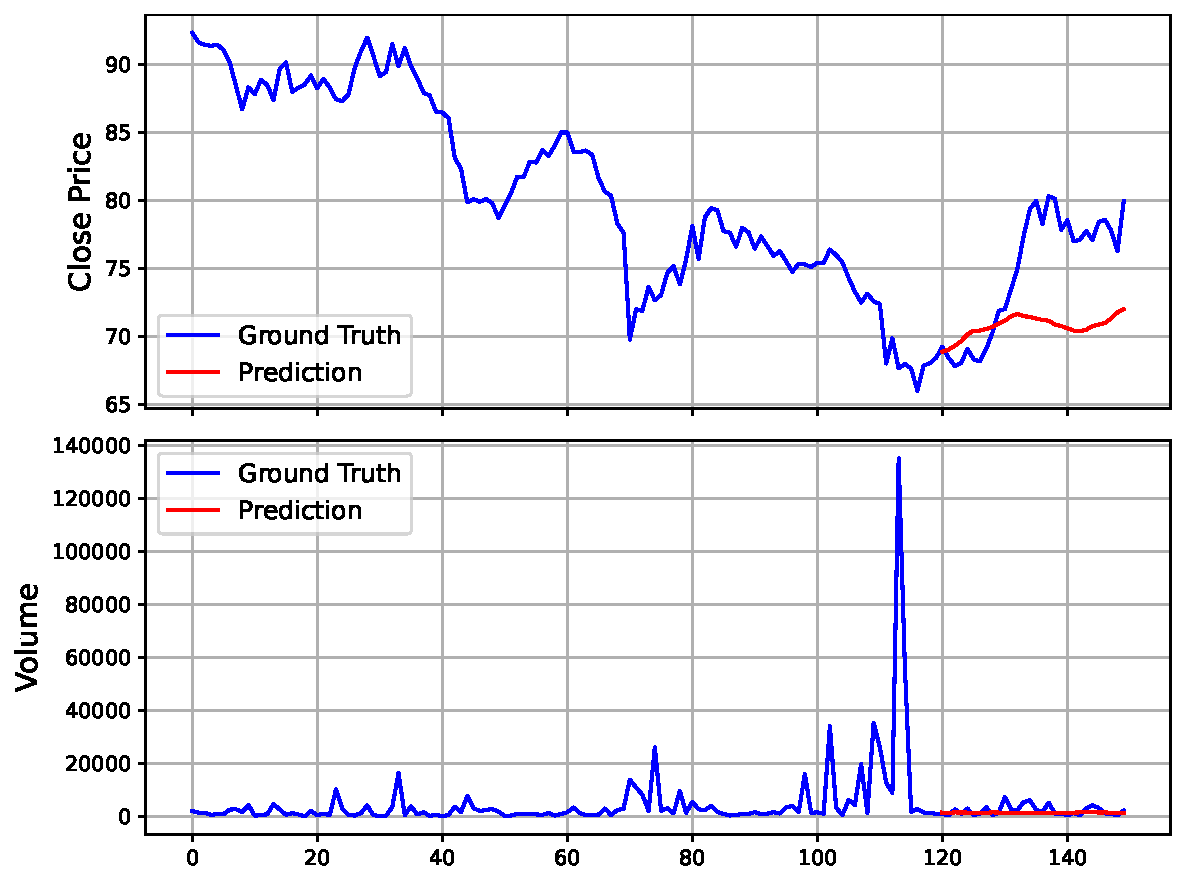
\includegraphics[width=\linewidth]{pred_imgs/pred_visualize_stock_XFRA_BMW_daily_Chronos_base.pdf}
        \caption{$\text{Chronos}_{base}$}
    \end{subfigure}
    \hfill
    \begin{subfigure}[b]{0.33\textwidth}
        \centering
        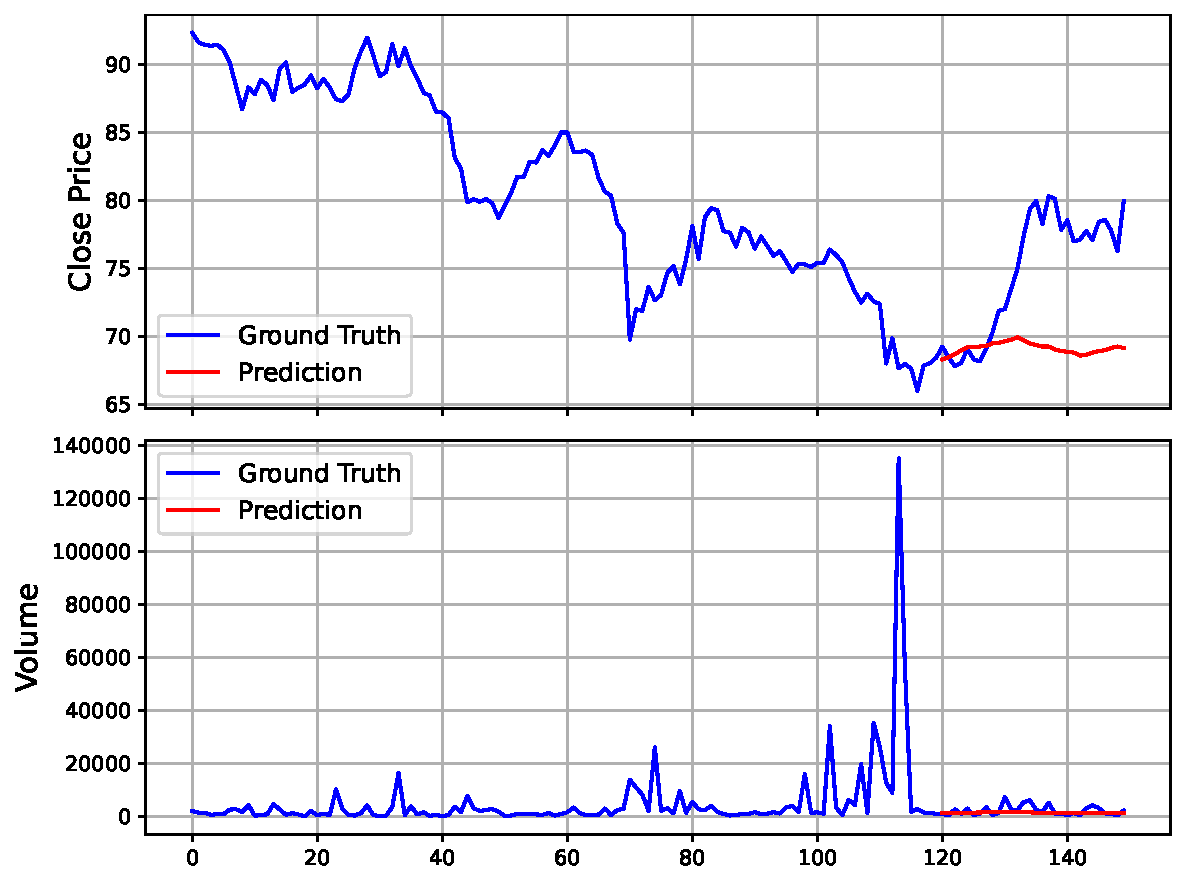
\includegraphics[width=\linewidth]{pred_imgs/pred_visualize_stock_XFRA_BMW_daily_Chronos_large.pdf}
        \caption{$\text{Chronos}_{large}$}
    \end{subfigure}

    \vspace{0.1cm}

    \begin{subfigure}[b]{0.33\textwidth}
        \centering
        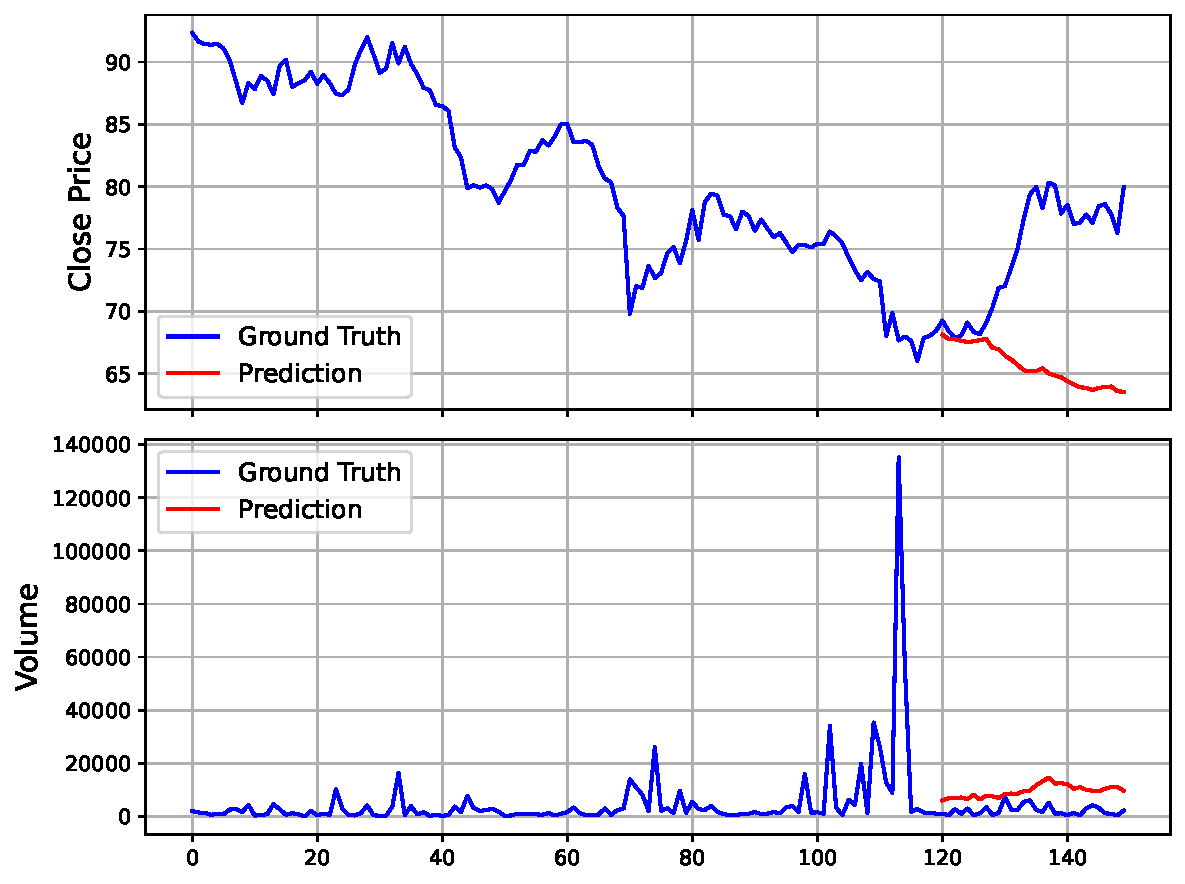
\includegraphics[width=\linewidth]{pred_imgs/pred_visualize_stock_XFRA_BMW_daily_iTransformer.pdf}
        \caption{iTransformer}
    \end{subfigure}
    \hfill
    \begin{subfigure}[b]{0.33\textwidth}
        \centering
        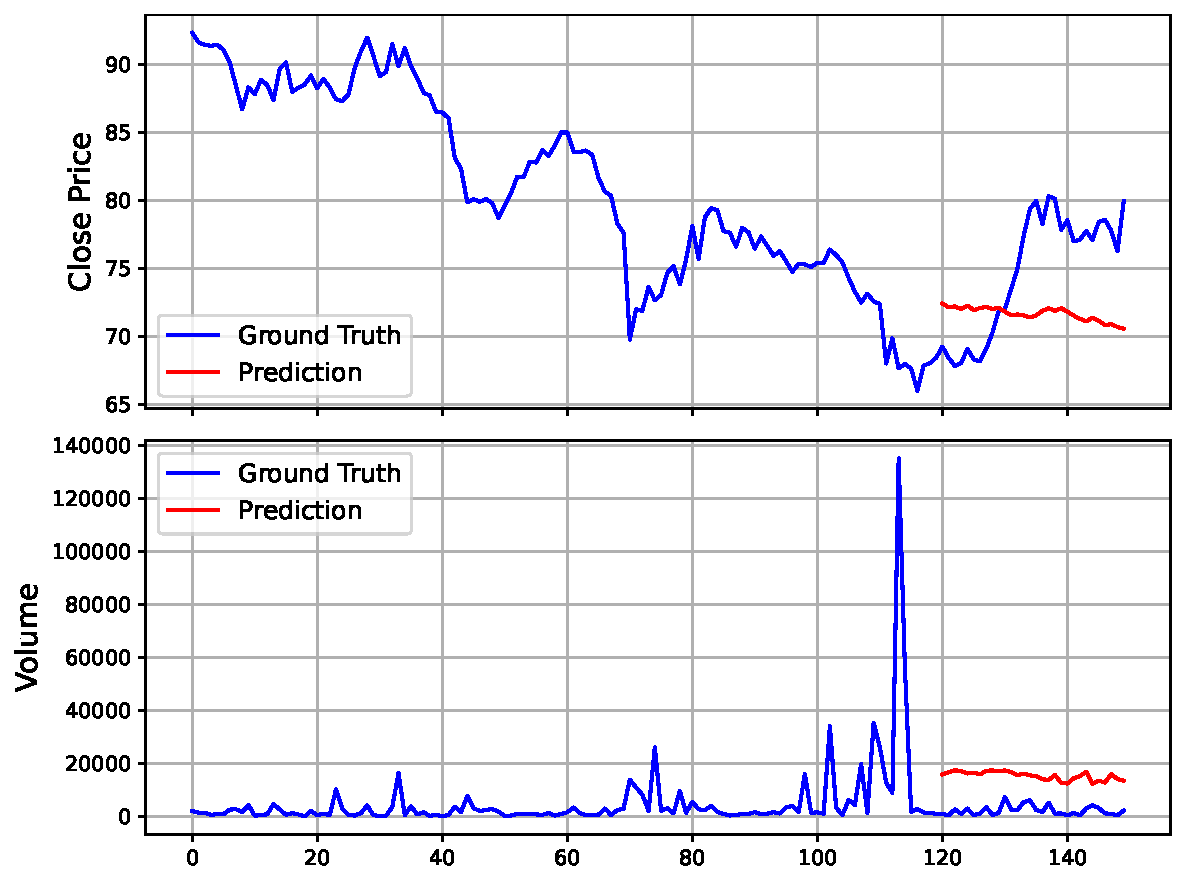
\includegraphics[width=\linewidth]{pred_imgs/pred_visualize_stock_XFRA_BMW_daily_DLinear.pdf}
        \caption{DLinear}
    \end{subfigure}
    \hfill
    \begin{subfigure}[b]{0.33\textwidth}
        \centering
        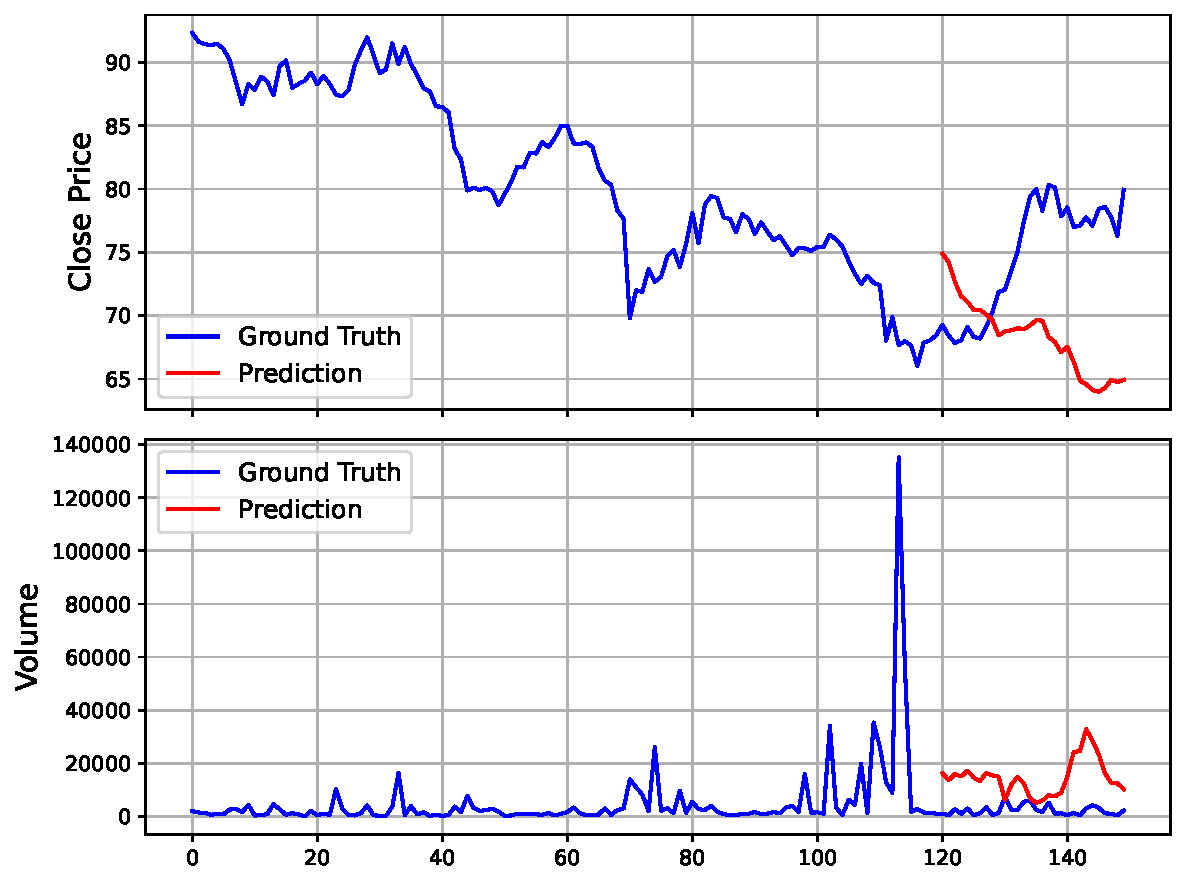
\includegraphics[width=\linewidth]{pred_imgs/pred_visualize_stock_XFRA_BMW_daily_TimesNet.pdf}
        \caption{TimesNet}
    \end{subfigure}

    \caption{일간 K-line 데이터를 기반으로 한 BMW (FWB: BMW)의 `Close Price'와 `Volume' 예측 결과. 모델은 120스텝 look-back 윈도우를 사용하여 30스텝 horizon을 예측한다. \textcolor{blue}{Blue} 선은 정답값을 나타내고 \textcolor{red}{red} 선은 모델의 예측값을 나타낸다.}
    \label{fig:pred_case_5}
\end{figure*}


\end{document}
